%slide 7 - cancel out - contasin out line of theoires - whihc?? - muon pature
\documentclass[12pt,a4paper]{report}

%\usepackage{fancyhdr}

%\pagestyle{fancy}

%\rhead{Share\LaTeX}
%\lhead{Guides and tutorials}
%\rfoot{Page \thepage}
\usepackage[T1]{fontenc}
\usepackage{kpfonts}


\usepackage{amsmath}
\newcommand{\Rn}[1]{%make roman
  \textup{\uppercase\expandafter{\romannumeral#1}}%
}
\newcommand*{\mybox}[1]{\framebox{#1}}
%\newcommand{\myboxcol}[2]{{\color{#1}\fbox{\normalcolor#2}}}
\newcommand*{\colorboxed}{}
\def\colorboxed#1#{%
  \colorboxedAux{#1}%
}
\newcommand*{\colorboxedAux}[3]{%
  % #1: optional argument for color model
  % #2: color specification
  % #3: formula
  \begingroup
    \colorlet{cb@saved}{.}%
    \color#1{#2}%
    \boxed{%
      \color{cb@saved}%
      #3%
    }%
  \endgroup
}

\usepackage{float}
%\usepackage{fancyhdr}
%\fancyhead[LE,RO]{foo}
%\fancyhead[LO,RE]{bar}
%\pagestyle{fancy}

\usepackage{amsfonts}
\usepackage{amssymb}
%\usepackage{bm}
\usepackage{fixmath}
%\usepackage{bm}
\usepackage{ifthen} % for conditional statements
\usepackage{subfig} %  Allows for subfigures
%\usepackage{subcaption} %  Allows for subfigures
\usepackage{dcolumn}
\usepackage{columntypes}
%\usepackage[a-3a]{pdfx}
\usepackage{upgreek}
\usepackage{color}
\usepackage[dvipsnames]{xcolor}
\definecolor{semigreen}{HTML}{1b9e77}
\definecolor{orangy}{HTML}{d95f02}
\definecolor{bluey}{HTML}{7570b3}
\usepackage[colorlinks = true, linkcolor = semigreen, citecolor = orangy]{hyperref}
\usepackage{gensymb}
%\usepackage{glossaries}
\newboolean{pdflatex}
\setboolean{pdflatex}{true} % False for eps figures 
\usepackage[section]{placeins}

\newboolean{articletitles}
\setboolean{articletitles}{true} % False removes titles in references

\newboolean{uprightparticles}
\setboolean{uprightparticles}{false} %True for upright particle symbols
\usepackage{mciteplus}
\newboolean{inbibliography}
\setboolean{inbibliography}{false} %
\usepackage{multirow}
%\usepackage{tocloft}
\linespread{1.5}
\newcommand{\mb}[1]{\mbox{\boldmath{$#1$}}}
\DeclareRobustCommand{\mb}[1]{\boldmath$#1$\unboldmath}
\usepackage{multirow,bigdelim}
%\usepackage{physics}
\usepackage{tikz}
\newcommand*\circledss[1]{\tikz[baseline=(math.base)]{\node[shape=circle,draw=green,text width=0.5cm] (math) {};}}
\newcommand*\circledsst[1]{\tikz[baseline=(math.base)]{\node[shape=circle,draw=red,text width=0.5cm] (math) {$#1$};}}
\newcommand*\circleds[1]{\tikz[baseline=(math.base)]{\node[shape=circle,draw=red,text width=1.0cm] (math) {$#1$};}}
\newcommand*\circledm[1]{\tikz[baseline=(math.base)]{\node[shape=circle,draw=yellow,text width=1.5cm] (math) {$#1$};}}
\newcommand*\circledb[1]{\tikz[baseline=(math.base)]{\node[shape=circle,draw=violet,text width=2cm] (math) {$#1$};}}

\newcommand*\circledimp[1]{\tikz[baseline=(math.base)]{\node[shape=circle,draw=green,text width=2cm] (math) {$#1$};}}
\newcommand*{\bfrac}[2]{\genfrac{}{}{0pt}{}{#1}{#2}}
%\usepackage{mathtools}
%\newcommand\mathcircled[1]{%
%  \mathpalette\@mathcircled{#1}%
%}
%\newcommand\@mathcircled[2]{%
%  \tikz[baseline=(math.base)] \node[draw,circle,inner sep=1pt] (math) {$\m@th#1#2$};%
%}


\usepackage{siunitx}
\usepackage{booktabs}
\usepackage[version=4]{mhchem}
\usepackage{collcell}

\newcolumntype{H}{@{}>{\lrbox0}l<{\endlrbox}}


%\usepackage[version=4]{mhchem}
%\renewcommand\cftchapfont{\boldfont}
%\renewcommand\cftchappagefont{\boldfont}
%% \usepackage{etoolbox}
%% \makeatletter
%% \patchcmd{\@dottedtocline}{\leavevmode}{\leavevmode\bfseries\boldmath}{}{}
%% \patchcmd{\@dottedtocline}{\normalfont}{\normalfont\bfseries\boldmath}{}{}
%% \patchcmd{\l@part}{\bfseries}{\bfseries\boldmath}{}{}
%% % \patchcmd{\l@chapter}{\bfseries}{\bfseries\boldmath}{}{}% report/book
%% \patchcmd{\l@section}{\bfseries}{\bfseries\boldmath}{}{}% article

%% \patchcmd{\@part}{\bfseries}{\bfseries\boldmath}{}{}
%% \patchcmd{\@spart}{\bfseries}{\bfseries\boldmath}{}{}
%% % \patchcmd{\@makechapterhead}{\bfseries}{\bfseries\boldmath}{}{}% report/book
%% % \patchcmd{\@makeschapterhead}{\bfseries}{\bfseries\boldmath}{}{}% % report/book
%% \patchcmd{\section}{\bfseries}{\bfseries\boldmath}{}{}
%% \patchcmd{\subsection}{\bfseries}{\bfseries\boldmath}{}{}
%% \patchcmd{\subsubsection}{\bfseries}{\bfseries\boldmath}{}{}
%% \patchcmd{\paragraph}{\bfseries}{\bfseries\boldmath}{}{}
%% \patchcmd{\subparagraph}{\bfseries}{\bfseries\boldmath}{}{}
%% \makeatother

%%\bfseries{\boldmath} 

% THis file contains all the default packages and modifications for
% LHCb formatting

%% %%%%%%%%%%%%%%%%%%
%%  Page formatting
%% %%%%%%%%%%%%%%%%%%
\textheight=230mm
\textwidth=160mm
\oddsidemargin=7mm
\evensidemargin=-10mm
\topmargin=-10mm
\headsep=20mm
\columnsep=5mm
\addtolength{\belowcaptionskip}{0.5em}

\renewcommand{\textfraction}{0.01}
\renewcommand{\floatpagefraction}{0.99}
\renewcommand{\topfraction}{0.9}
\renewcommand{\bottomfraction}{0.9}


\setlength{\hoffset}{-2cm}
\setlength{\voffset}{-2cm}
% Page defaults ...
\topmargin=0.5cm
\oddsidemargin=2.5cm
\textwidth=16cm
\textheight=22cm
% Allow the page size to vary a bit ...
\raggedbottom
% To avoid Latex to be too fussy with line breaking ...
\sloppy

\usepackage{fancyhdr}

\pagestyle{fancy}
%\fancyhead[LO,RE]{\leftmark}
\rhead{}
\lhead{\textbf{\leftmark}}
%\rfoot{Page \thepage}




%% %%%%%%%%%%%%%%%%%%%%%%%
%% Packages to be used
%% %%%%%%%%%%%%%%%%%%%%%%% 
\usepackage{microtype}
\usepackage{lineno}  % for line numbering during review
\usepackage{xspace} % To avoid problems with missing or double spaces after
                    % predefined symbold


%% Graphics
\usepackage{graphicx}  % to include figures (can also use other packages)
\usepackage{color}
\usepackage{colortbl}
\graphicspath{{./figs/}} % Make Latex search fig subdir for figures

%% Math
\usepackage{amsmath} % Adds a large collection of math symbols
\usepackage{amssymb}
\usepackage{amsfonts}
\usepackage{rotating}
\usepackage{mathtools}
%%\usepackage{upgreek} % Adds in support for greek letters in roman typeset

%% fix to allow peaceful coexistence of line numbering and
%% mathematical objects
%% http://www.latex-community.org/forum/viewtopic.php?f=5&t=163
%%
\newcommand*\patchAmsMathEnvironmentForLineno[1]{%
\expandafter\let\csname old#1\expandafter\endcsname\csname #1\endcsname
\expandafter\let\csname oldend#1\expandafter\endcsname\csname
end#1\endcsname
 \renewenvironment{#1}%
   {\linenomath\csname old#1\endcsname}%
   {\csname oldend#1\endcsname\endlinenomath}%
}
\newcommand*\patchBothAmsMathEnvironmentsForLineno[1]{%
  \patchAmsMathEnvironmentForLineno{#1}%
  \patchAmsMathEnvironmentForLineno{#1*}%
}
\AtBeginDocument{%
\patchBothAmsMathEnvironmentsForLineno{equation}%
\patchBothAmsMathEnvironmentsForLineno{align}%
\patchBothAmsMathEnvironmentsForLineno{flalign}%
\patchBothAmsMathEnvironmentsForLineno{alignat}%
\patchBothAmsMathEnvironmentsForLineno{gather}%
\patchBothAmsMathEnvironmentsForLineno{multline}%
}

% Get hyperlinks to captions and in references.
% These do not work with revtex. Use "hypertext" as class option instead.
\usepackage{hyperref}    % Hyperlinks in references
\usepackage[all]{hypcap} % Internal hyperlinks to floats.

%%% $Id: lhcb-symbols-def.tex 50511 2014-03-12 16:54:15Z pkoppenb $
%%% ======================================================================
%%% Purpose: Standard LHCb aliases
%%% Author: Originally Ulrik Egede, adapted by Tomasz Skwarnicki for templates,
%%% rewritten by Chris Parkes
%%% Maintainer : Ulrik Egede (2010 - 2012)
%%% =======================================================================

%%% To use this file outside the normal LHCb document environment, the
%%% following should be added in a preamble (before \begin{document}
%%%
%%%\usepackage{ifthen} 
%%%\newboolean{uprightparticles}
%%%\setboolean{uprightparticles}{false} %Set true for upright particle symbols
%%% \usepackage{xspace} 
%%% \usepackage{upgreek}

%%%%%%%%%%%%%%%%%%%%%%%%%%%%%%%%%%%%%%%%%%%%%%%%%%%%%%%%%%%%
%%%
%%% The following is to ensure that the template automatically can process
%%% this file.
%%%
%%% Add comments with at least three %%% preceding.
%%% Add new sections with one % preceding
%%% Add new subsections with two %% preceding
%%%%%%%%%%%%%%%%%%%%%%%%%%%%%%%%%%%%%%%%%%%%%%%%%%%%%%%%%%%%

%%%%%%%%%%%%%
% Experiments
%%%%%%%%%%%%%
\def\lhcb {\mbox{LHCb}\xspace}
\def\atlas  {\mbox{ATLAS}\xspace}
\def\cms    {\mbox{CMS}\xspace}
\def\alice  {\mbox{ALICE}\xspace}
\def\babar  {\mbox{BaBar}\xspace}
\def\belle  {\mbox{Belle}\xspace}
\def\cleo   {\mbox{CLEO}\xspace}
\def\cdf    {\mbox{CDF}\xspace}
\def\dzero  {\mbox{D0}\xspace}
\def\aleph  {\mbox{ALEPH}\xspace}
\def\delphi {\mbox{DELPHI}\xspace}
\def\opal   {\mbox{OPAL}\xspace}
\def\lthree {\mbox{L3}\xspace}
\def\sld    {\mbox{SLD}\xspace}
%%%\def\argus  {\mbox{ARGUS}\xspace}
%%%\def\uaone  {\mbox{UA1}\xspace}
%%%\def\uatwo  {\mbox{UA2}\xspace}
%%%\def\ux85 {\mbox{UX85}\xspace}
\def\cern {\mbox{CERN}\xspace}
\def\lhc    {\mbox{LHC}\xspace}
\def\lep    {\mbox{LEP}\xspace}
\def\tevatron {Tevatron\xspace}

%% LHCb sub-detectors and sub-systems

%%%\def\pu     {PU\xspace}
\def\velo   {VELO\xspace}
\def\rich   {RICH\xspace}
\def\richone {RICH1\xspace}
\def\richtwo {RICH2\xspace}
\def\ttracker {TT\xspace}
\def\intr   {IT\xspace}
\def\st     {ST\xspace}
\def\ot     {OT\xspace}
%%%\def\Tone   {T1\xspace}
%%%\def\Ttwo   {T2\xspace}
%%%\def\Tthree {T3\xspace}
%%%\def\Mone   {M1\xspace}
%%%\def\Mtwo   {M2\xspace}
%%%\def\Mthree {M3\xspace}
%%%\def\Mfour  {M4\xspace}
%%%\def\Mfive  {M5\xspace}
\def\spd    {SPD\xspace}
\def\presh  {PS\xspace}
\def\ecal   {ECAL\xspace}
\def\hcal   {HCAL\xspace}
%%%\def\bcm    {BCM\xspace}

%%%\def\ode    {ODE\xspace}
%%%\def\daq    {DAQ\xspace}
%%%\def\tfc    {TFC\xspace}
%%%\def\ecs    {ECS\xspace}
%%%\def\lone   {L0\xspace}
%%%\def\hlt    {HLT\xspace}
%%%\def\hltone {HLT1\xspace}
%%%\def\hlttwo {HLT2\xspace}

%%% Upright (not slanted) Particles

\ifthenelse{\boolean{uprightparticles}}%
{\def\Palpha      {\ensuremath{\upalpha}\xspace}
 \def\Pbeta       {\ensuremath{\upbeta}\xspace}
 \def\Pgamma      {\ensuremath{\upgamma}\xspace}                 
 \def\Pdelta      {\ensuremath{\updelta}\xspace}                 
 \def\Pepsilon    {\ensuremath{\upepsilon}\xspace}                 
 \def\Pvarepsilon {\ensuremath{\upvarepsilon}\xspace}                 
 \def\Pzeta       {\ensuremath{\upzeta}\xspace}                 
 \def\Peta        {\ensuremath{\upeta}\xspace}                 
 \def\Ptheta      {\ensuremath{\uptheta}\xspace}                 
 \def\Pvartheta   {\ensuremath{\upvartheta}\xspace}                 
 \def\Piota       {\ensuremath{\upiota}\xspace}                 
 \def\Pkappa      {\ensuremath{\upkappa}\xspace}                 
 \def\Plambda     {\ensuremath{\uplambda}\xspace}                 
 \def\Pmu         {\ensuremath{\upmu}\xspace}                 
 \def\Pnu         {\ensuremath{\upnu}\xspace}                 
 \def\Pxi         {\ensuremath{\upxi}\xspace}                 
 \def\Ppi         {\ensuremath{\uppi}\xspace}                 
 \def\Pvarpi      {\ensuremath{\upvarpi}\xspace}                 
 \def\Prho        {\ensuremath{\uprho}\xspace}                 
 \def\Pvarrho     {\ensuremath{\upvarrho}\xspace}                 
 \def\Ptau        {\ensuremath{\uptau}\xspace}                 
 \def\Pupsilon    {\ensuremath{\upupsilon}\xspace}                 
 \def\Pphi        {\ensuremath{\upphi}\xspace}                 
 \def\Pvarphi     {\ensuremath{\upvarphi}\xspace}                 
 \def\Pchi        {\ensuremath{\upchi}\xspace}                 
 \def\Ppsi        {\ensuremath{\uppsi}\xspace}                 
 \def\Pomega      {\ensuremath{\upomega}\xspace}                 

 \def\PDelta      {\ensuremath{\Delta}\xspace}                 
 \def\PXi      {\ensuremath{\Xi}\xspace}                 
 \def\PLambda      {\ensuremath{\Lmbda}\xspace}                 
 \def\PSigma      {\ensuremath{\Sigma}\xspace}                 
 \def\POmega      {\ensuremath{\Omega}\xspace}                 
 \def\PUpsilon      {\ensuremath{\Upsilon}\xspace}                 
 
 %\mathchardef\Deltares="7101
 %\mathchardef\Xi="7104
 %\mathchardef\Lambda="7103
 %\mathchardef\Sigma="7106
 %\mathchardef\Omega="710A


 \def\PA      {\ensuremath{\mathrm{A}}\xspace}                 
 \def\PB      {\ensuremath{\mathrm{B}}\xspace}                 
 \def\PC      {\ensuremath{\mathrm{C}}\xspace}                 
 \def\PD      {\ensuremath{\mathrm{D}}\xspace}                 
 \def\PE      {\ensuremath{\mathrm{E}}\xspace}                 
 \def\PF      {\ensuremath{\mathrm{F}}\xspace}                 
 \def\PG      {\ensuremath{\mathrm{G}}\xspace}                 
 \def\PH      {\ensuremath{\mathrm{H}}\xspace}                 
 \def\PI      {\ensuremath{\mathrm{I}}\xspace}                 
 \def\PJ      {\ensuremath{\mathrm{J}}\xspace}                 
 \def\PK      {\ensuremath{\mathrm{K}}\xspace}                 
 \def\PL      {\ensuremath{\mathrm{L}}\xspace}                 
 \def\PM      {\ensuremath{\mathrm{M}}\xspace}                 
 \def\PN      {\ensuremath{\mathrm{N}}\xspace}                 
 \def\PO      {\ensuremath{\mathrm{O}}\xspace}                 
 \def\PP      {\ensuremath{\mathrm{P}}\xspace}                 
 \def\PQ      {\ensuremath{\mathrm{Q}}\xspace}                 
 \def\PR      {\ensuremath{\mathrm{R}}\xspace}                 
 \def\PS      {\ensuremath{\mathrm{S}}\xspace}                 
 \def\PT      {\ensuremath{\mathrm{T}}\xspace}                 
 \def\PU      {\ensuremath{\mathrm{U}}\xspace}                 
 \def\PV      {\ensuremath{\mathrm{V}}\xspace}                 
 \def\PW      {\ensuremath{\mathrm{W}}\xspace}                 
 \def\PX      {\ensuremath{\mathrm{X}}\xspace}                 
 \def\PY      {\ensuremath{\mathrm{Y}}\xspace}                 
 \def\PZ      {\ensuremath{\mathrm{Z}}\xspace}                 
 \def\Pa      {\ensuremath{\mathrm{a}}\xspace}                 
 \def\Pb      {\ensuremath{\mathrm{b}}\xspace}                 
 \def\Pc      {\ensuremath{\mathrm{c}}\xspace}                 
 \def\Pd      {\ensuremath{\mathrm{d}}\xspace}                 
 \def\Pe      {\ensuremath{\mathrm{e}}\xspace}                 
 \def\Pf      {\ensuremath{\mathrm{f}}\xspace}                 
 \def\Pg      {\ensuremath{\mathrm{g}}\xspace}                 
 \def\Ph      {\ensuremath{\mathrm{h}}\xspace}                 
 \def\Pi      {\ensuremath{\mathrm{i}}\xspace}                 
 \def\Pj      {\ensuremath{\mathrm{j}}\xspace}                 
 \def\Pk      {\ensuremath{\mathrm{k}}\xspace}                 
 \def\Pl      {\ensuremath{\mathrm{l}}\xspace}                 
 \def\Pm      {\ensuremath{\mathrm{m}}\xspace}                 
 \def\Pn      {\ensuremath{\mathrm{n}}\xspace}                 
 \def\Po      {\ensuremath{\mathrm{o}}\xspace}                 
 \def\Pp      {\ensuremath{\mathrm{p}}\xspace}                 
 \def\Pq      {\ensuremath{\mathrm{q}}\xspace}                 
 \def\Pr      {\ensuremath{\mathrm{r}}\xspace}                 
 \def\Ps      {\ensuremath{\mathrm{s}}\xspace}                 
 \def\Pt      {\ensuremath{\mathrm{t}}\xspace}                 
 \def\Pu      {\ensuremath{\mathrm{u}}\xspace}                 
 \def\Pv      {\ensuremath{\mathrm{v}}\xspace}                 
 \def\Pw      {\ensuremath{\mathrm{w}}\xspace}                 
 \def\Px      {\ensuremath{\mathrm{x}}\xspace}                 
 \def\Py      {\ensuremath{\mathrm{y}}\xspace}                 
 \def\Pz      {\ensuremath{\mathrm{z}}\xspace}                 
}
{\def\Palpha      {\ensuremath{\alpha}\xspace}
 \def\Pbeta       {\ensuremath{\beta}\xspace}
 \def\Pgamma      {\ensuremath{\gamma}\xspace}                 
 \def\Pdelta      {\ensuremath{\delta}\xspace}                 
 \def\Pepsilon    {\ensuremath{\epsilon}\xspace}                 
 \def\Pvarepsilon {\ensuremath{\varepsilon}\xspace}                 
 \def\Pzeta       {\ensuremath{\zeta}\xspace}                 
 \def\Peta        {\ensuremath{\eta}\xspace}                 
 \def\Ptheta      {\ensuremath{\theta}\xspace}                 
 \def\Pvartheta   {\ensuremath{\vartheta}\xspace}                 
 \def\Piota       {\ensuremath{\iota}\xspace}                 
 \def\Pkappa      {\ensuremath{\kappa}\xspace}                 
 \def\Plambda     {\ensuremath{\lambda}\xspace}                 
 \def\Pmu         {\ensuremath{\mu}\xspace}                 
 \def\Pnu         {\ensuremath{\nu}\xspace}                 
 \def\Pxi         {\ensuremath{\xi}\xspace}                 
 \def\Ppi         {\ensuremath{\pi}\xspace}                 
 \def\Pvarpi      {\ensuremath{\varpi}\xspace}                 
 \def\Prho        {\ensuremath{\rho}\xspace}                 
 \def\Pvarrho     {\ensuremath{\varrho}\xspace}                 
 \def\Ptau        {\ensuremath{\tau}\xspace}                 
 \def\Pupsilon    {\ensuremath{\upsilon}\xspace}                 
 \def\Pphi        {\ensuremath{\phi}\xspace}                 
 \def\Pvarphi     {\ensuremath{\varphi}\xspace}                 
 \def\Pchi        {\ensuremath{\chi}\xspace}                 
 \def\Ppsi        {\ensuremath{\psi}\xspace}                 
 \def\Pomega      {\ensuremath{\omega}\xspace}                 
 \mathchardef\PDelta="7101
 \mathchardef\PXi="7104
 \mathchardef\PLambda="7103
 \mathchardef\PSigma="7106
 \mathchardef\POmega="710A
 \mathchardef\PUpsilon="7107
 \def\PA      {\ensuremath{A}\xspace}                 
 \def\PB      {\ensuremath{B}\xspace}                 
 \def\PC      {\ensuremath{C}\xspace}                 
 \def\PD      {\ensuremath{D}\xspace}                 
 \def\PE      {\ensuremath{E}\xspace}                 
 \def\PF      {\ensuremath{F}\xspace}                 
 \def\PG      {\ensuremath{G}\xspace}                 
 \def\PH      {\ensuremath{H}\xspace}                 
 \def\PI      {\ensuremath{I}\xspace}                 
 \def\PJ      {\ensuremath{J}\xspace}                 
 \def\PK      {\ensuremath{K}\xspace}                 
 \def\PL      {\ensuremath{L}\xspace}                 
 \def\PM      {\ensuremath{M}\xspace}                 
 \def\PN      {\ensuremath{N}\xspace}                 
 \def\PO      {\ensuremath{O}\xspace}                 
 \def\PP      {\ensuremath{P}\xspace}                 
 \def\PQ      {\ensuremath{Q}\xspace}                 
 \def\PR      {\ensuremath{R}\xspace}                 
 \def\PS      {\ensuremath{S}\xspace}                 
 \def\PT      {\ensuremath{T}\xspace}                 
 \def\PU      {\ensuremath{U}\xspace}                 
 \def\PV      {\ensuremath{V}\xspace}                 
 \def\PW      {\ensuremath{W}\xspace}                 
 \def\PX      {\ensuremath{X}\xspace}                 
 \def\PY      {\ensuremath{Y}\xspace}                 
 \def\PZ      {\ensuremath{Z}\xspace}                 
 \def\Pa      {\ensuremath{a}\xspace}                 
 \def\Pb      {\ensuremath{b}\xspace}                 
 \def\Pc      {\ensuremath{c}\xspace}                 
 \def\Pd      {\ensuremath{d}\xspace}                 
 \def\Pe      {\ensuremath{e}\xspace}                 
 \def\Pf      {\ensuremath{f}\xspace}                 
 \def\Pg      {\ensuremath{g}\xspace}                 
 \def\Ph      {\ensuremath{h}\xspace}                 
 \def\Pi      {\ensuremath{i}\xspace}                 
 \def\Pj      {\ensuremath{j}\xspace}                 
 \def\Pk      {\ensuremath{k}\xspace}                 
 \def\Pl      {\ensuremath{l}\xspace}                 
 \def\Pm      {\ensuremath{m}\xspace}                 
 \def\Pn      {\ensuremath{n}\xspace}                 
 \def\Po      {\ensuremath{o}\xspace}                 
 \def\Pp      {\ensuremath{p}\xspace}                 
 \def\Pq      {\ensuremath{q}\xspace}                 
 \def\Pr      {\ensuremath{r}\xspace}                 
 \def\Ps      {\ensuremath{s}\xspace}                 
 \def\Pt      {\ensuremath{t}\xspace}                 
 \def\Pu      {\ensuremath{u}\xspace}                 
 \def\Pv      {\ensuremath{v}\xspace}                 
 \def\Pw      {\ensuremath{w}\xspace}                 
 \def\Px      {\ensuremath{x}\xspace}                 
 \def\Py      {\ensuremath{y}\xspace}                 
 \def\Pz      {\ensuremath{z}\xspace}                 
}

%%%%%%%%%%%%%%%%%%%%%%%%%%%%%%%%%%%%%%%%%%%%%%%
% Particles

%% Leptons

\let\emi\en
\def\electron   {{\ensuremath{\Pe}}\xspace}
\def\en         {{\ensuremath{\Pe^-}}\xspace}   % electron negative (\em is taken)
\def\ep         {{\ensuremath{\Pe^+}}\xspace}
\def\epm        {{\ensuremath{\Pe^\pm}}\xspace} 
\def\epem       {{\ensuremath{\Pe^+\Pe^-}}\xspace}
%%%\def\ee         {\ensuremath{\Pe^-\Pe^-}\xspace}

\def\muon       {{\ensuremath{\Pmu}}\xspace}
\def\mup        {{\ensuremath{\Pmu^+}}\xspace}
\def\mun        {{\ensuremath{\Pmu^-}}\xspace} % muon negative (\mum is taken)
\def\mumu       {{\ensuremath{\Pmu^+\Pmu^-}}\xspace}
\def\mumumu       {{\ensuremath{\Pmu^+\Pmu^-\Pmu^+}}\xspace}

\def\tauon      {{\ensuremath{\Ptau}}\xspace}
\def\taup       {{\ensuremath{\Ptau^+}}\xspace}
\def\taum       {{\ensuremath{\Ptau^-}}\xspace}
\def\tautau     {{\ensuremath{\Ptau^+\Ptau^-}}\xspace}

\def\lepton     {{\ensuremath{\ell}}\xspace}
\def\ellm       {{\ensuremath{\ell^-}}\xspace}
\def\ellp       {{\ensuremath{\ell^+}}\xspace}
%%%\def\ellell     {\ensuremath{\ell^+ \ell^-}\xspace}

\def\neu        {{\ensuremath{\Pnu}}\xspace}
\def\neub       {{\ensuremath{\overline{\Pnu}}}\xspace}
%%%\def\nuenueb    {\ensuremath{\neu\neub}\xspace}
\def\neue       {{\ensuremath{\neu_e}}\xspace}
\def\neueb      {{\ensuremath{\neub_e}}\xspace}
%%%\def\neueneueb  {\ensuremath{\neue\neueb}\xspace}
\def\neum       {{\ensuremath{\neu_\mu}}\xspace}
\def\neumb      {{\ensuremath{\neub_\mu}}\xspace}
%%%\def\neumneumb  {\ensuremath{\neum\neumb}\xspace}
\def\neut       {{\ensuremath{\neu_\tau}}\xspace}
\def\neutb      {{\ensuremath{\neub_\tau}}\xspace}
%%%\def\neutneutb  {\ensuremath{\neut\neutb}\xspace}
\def\neul       {{\ensuremath{\neu_\ell}}\xspace}
\def\neulb      {{\ensuremath{\neub_\ell}}\xspace}
%%%\def\neulneulb  {\ensuremath{\neul\neulb}\xspace}

%% Gauge bosons and scalars

\def\g      {{\ensuremath{\Pgamma}}\xspace}
\def\H      {{\ensuremath{\PH^0}}\xspace}
\def\Hp     {{\ensuremath{\PH^+}}\xspace}
\def\Hm     {{\ensuremath{\PH^-}}\xspace}
\def\Hpm    {{\ensuremath{\PH^\pm}}\xspace}
\def\W      {{\ensuremath{\PW}}\xspace}
\def\Wp     {{\ensuremath{\PW^+}}\xspace}
\def\Wm     {{\ensuremath{\PW^-}}\xspace}
\def\Wpm    {{\ensuremath{\PW^\pm}}\xspace}
\def\Z      {{\ensuremath{\PZ}}\xspace}

%% Quarks

\def\quark     {{\ensuremath{\Pq}}\xspace}
\def\quarkbar  {{\ensuremath{\overline \quark}}\xspace}
\def\qqbar     {{\ensuremath{\quark\quarkbar}}\xspace}
\def\uquark    {{\ensuremath{\Pu}}\xspace}
\def\uquarkbar {{\ensuremath{\overline \uquark}}\xspace}
\def\uubar     {{\ensuremath{\uquark\uquarkbar}}\xspace}
\def\dquark    {{\ensuremath{\Pd}}\xspace}
\def\dquarkbar {{\ensuremath{\overline \dquark}}\xspace}
\def\ddbar     {{\ensuremath{\dquark\dquarkbar}}\xspace}
\def\squark    {{\ensuremath{\Ps}}\xspace}
\def\squarkbar {{\ensuremath{\overline \squark}}\xspace}
\def\ssbar     {{\ensuremath{\squark\squarkbar}}\xspace}
\def\cquark    {{\ensuremath{\Pc}}\xspace}
\def\cquarkbar {{\ensuremath{\overline \cquark}}\xspace}
\def\ccbar     {{\ensuremath{\cquark\cquarkbar}}\xspace}
\def\bquark    {{\ensuremath{\Pb}}\xspace}
\def\bquarkbar {{\ensuremath{\overline \bquark}}\xspace}
\def\bbbar     {{\ensuremath{\bquark\bquarkbar}}\xspace}
\def\tquark    {{\ensuremath{\Pt}}\xspace}
\def\tquarkbar {{\ensuremath{\overline \tquark}}\xspace}
\def\ttbar     {{\ensuremath{\tquark\tquarkbar}}\xspace}

%% Light mesons

\def\hadron {{\ensuremath{\Ph}}\xspace}
\def\pion   {{\ensuremath{\Ppi}}\xspace}
\def\piz    {{\ensuremath{\pion^0}}\xspace}
\def\pizs   {{\ensuremath{\pion^0\mbox\,\rm{s}}}\xspace}
\def\pip    {{\ensuremath{\pion^+}}\xspace}
\def\pim    {{\ensuremath{\pion^-}}\xspace}
\def\pimB    {{\ensuremath{\bf{\pion^-}}}\xspace}
\def\pipm   {{\ensuremath{\pion^\pm}}\xspace}
\def\pimp   {{\ensuremath{\pion^\mp}}\xspace}

\def\rhomeson {{\ensuremath{\Prho}}\xspace}
\def\rhoz     {{\ensuremath{\rhomeson^0}}\xspace}
\def\rhop     {{\ensuremath{\rhomeson^+}}\xspace}
\def\rhom     {{\ensuremath{\rhomeson^-}}\xspace}
\def\rhopm    {{\ensuremath{\rhomeson^\pm}}\xspace}
\def\rhomp    {{\ensuremath{\rhomeson^\mp}}\xspace}

\def\kaon    {{\ensuremath{\PK}}\xspace}
%%% do NOT use ensuremath here
  \def\Kbar    {{\kern 0.2em\overline{\kern -0.2em \PK}{}}\xspace}
\def\Kb      {{\ensuremath{\Kbar}}\xspace}
\def\Kz      {{\ensuremath{\kaon^0}}\xspace}
\def\Kzb     {{\ensuremath{\Kbar^0}}\xspace}
\def\Kp      {{\ensuremath{\kaon^+}}\xspace}
\def\Km      {{\ensuremath{\kaon^-}}\xspace}
\def\Kpm     {{\ensuremath{\kaon^\pm}}\xspace}
\def\Kmp     {{\ensuremath{\kaon^\mp}}\xspace}
%\def\KS      {{\ensuremath{\kaon^0_{\rm\scriptscriptstyle S}}}\xspace}
\def\KS      {{\ensuremath{\kaon^0_{s}}}\xspace}
\def\KSB     {{\ensuremath{\bf{\kaon^0_{\rm\scriptscriptstyle S}}}\xspace}}
\def\KL      {{\ensuremath{\kaon^0_{\rm\scriptscriptstyle L}}}\xspace}
\def\Kstarz  {{\ensuremath{\kaon^{*0}}}\xspace}
\def\Kstarzb {{\ensuremath{\Kbar^{*0}}}\xspace}
\def\Kstar   {{\ensuremath{\kaon^*}}\xspace}
\def\Kstarb  {{\ensuremath{\Kbar^*}}\xspace}
\def\Kstarp  {{\ensuremath{\kaon^{*+}}}\xspace}
\def\Kstarm  {{\ensuremath{\kaon^{*-}}}\xspace}
\def\Kstarpm {{\ensuremath{\kaon^{*\pm}}}\xspace}
\def\Kstarmp {{\ensuremath{\kaon^{*\mp}}}\xspace}

\newcommand{\etaz}{\ensuremath{\Peta}\xspace}
\newcommand{\etapr}{\ensuremath{\Peta^{\prime}}\xspace}
\newcommand{\phiz}{\ensuremath{\Pphi}\xspace}
\newcommand{\omegaz}{\ensuremath{\Pomega}\xspace}

%% Heavy mesons

%%% do NOT use ensuremath here
  \def\Dbar    {{\kern 0.2em\overline{\kern -0.2em \PD}{}}\xspace}
\def\D       {{\ensuremath{\PD}}\xspace}
\def\Db      {{\ensuremath{\Dbar}}\xspace}
\def\Dz      {{\ensuremath{\D^0}}\xspace}
\def\Dzb     {{\ensuremath{\Dbar^0}}\xspace}
\def\Dp      {{\ensuremath{\D^+}}\xspace}
\def\Dm      {{\ensuremath{\D^-}}\xspace}
\def\Dpm     {{\ensuremath{\D^\pm}}\xspace}
\def\Dmp     {{\ensuremath{\D^\mp}}\xspace}
\def\Dstar   {{\ensuremath{\D^*}}\xspace}
\def\Dstarb  {{\ensuremath{\Dbar^*}}\xspace}
\def\Dstarz  {{\ensuremath{\D^{*0}}}\xspace}
\def\Dstarzb {{\ensuremath{\Dbar^{*0}}}\xspace}
\def\Dstarp  {{\ensuremath{\D^{*+}}}\xspace}
\def\Dstarm  {{\ensuremath{\D^{*-}}}\xspace}
\def\Dstarpm {{\ensuremath{\D^{*\pm}}}\xspace}
\def\Dstarmp {{\ensuremath{\D^{*\mp}}}\xspace}
\def\Ds      {{\ensuremath{\D^+_\squark}}\xspace}
\def\Dsp     {{\ensuremath{\D^+_\squark}}\xspace}
\def\Dsm     {{\ensuremath{\D^-_\squark}}\xspace}
\def\Dspm    {{\ensuremath{\D^{\pm}_\squark}}\xspace}
\def\Dsmp    {{\ensuremath{\D^{\mp}_\squark}}\xspace}
\def\Dss     {{\ensuremath{\D^{*+}_\squark}}\xspace}
\def\Dssp    {{\ensuremath{\D^{*+}_\squark}}\xspace}
\def\Dssm    {{\ensuremath{\D^{*-}_\squark}}\xspace}
\def\Dsspm   {{\ensuremath{\D^{*\pm}_\squark}}\xspace}
\def\Dssmp   {{\ensuremath{\D^{*\mp}_\squark}}\xspace}

\def\B       {{\ensuremath{\PB}}\xspace}
%%% do NOT use ensuremath here
\def\Bbar    {{\ensuremath{\kern 0.18em\overline{\kern -0.18em \PB}{}}}\xspace}
\def\Bb      {{\ensuremath{\Bbar}}\xspace}
\def\Bz      {{\ensuremath{\B^0}}\xspace}
\def\Bzb     {{\ensuremath{\Bbar^0}}\xspace}
\def\Bu      {{\ensuremath{\B^+}}\xspace}
\def\Bub     {{\ensuremath{\B^-}}\xspace}
\def\Bp      {{\ensuremath{\Bu}}\xspace}
\def\Bm      {{\ensuremath{\Bub}}\xspace}
\def\Bpm     {{\ensuremath{\B^\pm}}\xspace}
\def\Bmp     {{\ensuremath{\B^\mp}}\xspace}
\def\Bd      {{\ensuremath{\B^0}}\xspace}
\def\Bs      {{\ensuremath{\B^0_\squark}}\xspace}
\def\Bsb     {{\ensuremath{\Bbar^0_\squark}}\xspace}
\def\Bdb     {{\ensuremath{\Bbar^0}}\xspace}
\def\Bc      {{\ensuremath{\B_\cquark^+}}\xspace}
\def\Bcp     {{\ensuremath{\B_\cquark^+}}\xspace}
\def\Bcm     {{\ensuremath{\B_\cquark^-}}\xspace}
\def\Bcpm    {{\ensuremath{\B_\cquark^\pm}}\xspace}

%% Onia

\def\jpsi     {{\ensuremath{{\PJ\mskip -3mu/\mskip -2mu\Ppsi\mskip 2mu}}}\xspace}
\def\psitwos  {{\ensuremath{\Ppsi{(2S)}}}\xspace}
\def\psiprpr  {{\ensuremath{\Ppsi(3770)}}\xspace}
\def\etac     {{\ensuremath{\Peta_\cquark}}\xspace}
\def\chiczero {{\ensuremath{\Pchi_{\cquark 0}}}\xspace}
\def\chicone  {{\ensuremath{\Pchi_{\cquark 1}}}\xspace}
\def\chictwo  {{\ensuremath{\Pchi_{\cquark 2}}}\xspace}
  %\mathchardef\Upsilon="7107
  \def\Y#1S{\ensuremath{\PUpsilon{(#1S)}}\xspace}% no space before {...}!
\def\OneS  {{\Y1S}}
\def\TwoS  {{\Y2S}}
\def\ThreeS{{\Y3S}}
\def\FourS {{\Y4S}}
\def\FiveS {{\Y5S}}

\def\chic  {{\ensuremath{\Pchi_{c}}}\xspace}

%% Baryons

\def\proton      {{\ensuremath{\Pp}}\xspace}
\def\antiproton  {{\ensuremath{\overline \proton}}\xspace}
\def\neutron     {{\ensuremath{\Pn}}\xspace}
\def\antineutron {{\ensuremath{\overline \neutron}}\xspace}
\def\Deltares    {{\ensuremath{\PDelta}}\xspace}
\def\Deltaresbar {{\ensuremath{\overline \Deltares}}\xspace}
\def\Xires       {{\ensuremath{\PXi}}\xspace}
\def\Xiresbar    {{\ensuremath{\overline \Xires}}\xspace}
\def\Lz          {{\ensuremath{\PLambda^0}}\xspace}
\def\Lbar        {{\ensuremath{\kern 0.1em\overline{\kern -0.1em\PLambda}}}\xspace}
\def\Lambdares   {{\ensuremath{\PLambda}}\xspace}
\def\Lambdaresbar{{\ensuremath{\Lbar}}\xspace}
\def\Sigmares    {{\ensuremath{\PSigma}}\xspace}
\def\Sigmaresbar {{\ensuremath{\overline \Sigmares}}\xspace}
\def\Omegares    {{\ensuremath{\POmega^-}}\xspace}
\def\Omegaresbar {{\ensuremath{\overline{\POmega}^+}}\xspace}

%%% do NOT use ensuremath here
 % \def\Deltabar{\kern 0.25em\overline{\kern -0.25em \Deltares}{}\xspace}
 % \def\Sigbar{\kern 0.2em\overline{\kern -0.2em \Sigma}{}\xspace}
 % \def\Xibar{\kern 0.2em\overline{\kern -0.2em \Xi}{}\xspace}
 % \def\Obar{\kern 0.2em\overline{\kern -0.2em \Omega}{}\xspace}
 % \def\Nbar{\kern 0.2em\overline{\kern -0.2em N}{}\xspace}
 % \def\Xb{\kern 0.2em\overline{\kern -0.2em X}{}\xspace}

\def\Lb      {{\ensuremath{\PLambda^0_\bquark}}\xspace}
\def\Lbbar   {{\ensuremath{\Lbar^0_\bquark}}\xspace}
\def\Lc      {{\ensuremath{\PLambda^+_\cquark}}\xspace}
\def\Lcbar   {{\ensuremath{\Lbar^-_\cquark}}\xspace}

%%%%%%%%%%%%%%%%%%
% Physics symbols
%%%%%%%%%%%%%%%%%

%% Decays
\def\BF         {{\ensuremath{\cal B}}\xspace}
\def\BRvis      {{\ensuremath{\BR_{\rm{vis}}}}}
\def\BR         {\BF}
\newcommand{\decay}[2]{\ensuremath{#1\!\to #2}\xspace}         % {\Pa}{\Pb \Pc}
\def\ra                 {\ensuremath{\rightarrow}\xspace}
\def\to                 {\ensuremath{\rightarrow}\xspace}

%% Lifetimes
\newcommand{\tauBs}{{\ensuremath{\tau_{\Bs}}}\xspace}
\newcommand{\tauBd}{{\ensuremath{\tau_{\Bd}}}\xspace}
\newcommand{\tauBz}{{\ensuremath{\tau_{\Bz}}}\xspace}
\newcommand{\tauBu}{{\ensuremath{\tau_{\Bp}}}\xspace}
\newcommand{\tauDp}{{\ensuremath{\tau_{\Dp}}}\xspace}
\newcommand{\tauDz}{{\ensuremath{\tau_{\Dz}}}\xspace}
\newcommand{\tauL}{{\ensuremath{\tau_{\rm L}}}\xspace}
\newcommand{\tauH}{{\ensuremath{\tau_{\rm H}}}\xspace}

%% Masses
\newcommand{\mBd}{{\ensuremath{m_{\Bd}}}\xspace}
\newcommand{\mBp}{{\ensuremath{m_{\Bp}}}\xspace}
\newcommand{\mBs}{{\ensuremath{m_{\Bs}}}\xspace}
\newcommand{\mBc}{{\ensuremath{m_{\Bc}}}\xspace}
\newcommand{\mLb}{{\ensuremath{m_{\Lb}}}\xspace}

%% EW theory, groups
\def\grpsuthree {{\ensuremath{\mathrm{SU}(3)}}\xspace}
\def\grpsutw    {{\ensuremath{\mathrm{SU}(2)}}\xspace}
\def\grpuone    {{\ensuremath{\mathrm{U}(1)}}\xspace}

\def\ssqtw   {{\ensuremath{\sin^{2}\!\theta_{\mathrm{W}}}}\xspace}
\def\csqtw   {{\ensuremath{\cos^{2}\!\theta_{\mathrm{W}}}}\xspace}
\def\stw     {{\ensuremath{\sin\theta_{\mathrm{W}}}}\xspace}
\def\ctw     {{\ensuremath{\cos\theta_{\mathrm{W}}}}\xspace}
\def\ssqtwef {{\ensuremath{{\sin}^{2}\theta_{\mathrm{W}}^{\mathrm{eff}}}}\xspace}
\def\csqtwef {{\ensuremath{{\cos}^{2}\theta_{\mathrm{W}}^{\mathrm{eff}}}}\xspace}
\def\stwef   {{\ensuremath{\sin\theta_{\mathrm{W}}^{\mathrm{eff}}}}\xspace}
\def\ctwef   {{\ensuremath{\cos\theta_{\mathrm{W}}^{\mathrm{eff}}}}\xspace}
\def\gv      {{\ensuremath{g_{\mbox{\tiny V}}}}\xspace}
\def\ga      {{\ensuremath{g_{\mbox{\tiny A}}}}\xspace}

\def\order   {{\ensuremath{\mathcal{O}}}\xspace}
\def\ordalph {{\ensuremath{\mathcal{O}(\alpha)}}\xspace}
\def\ordalsq {{\ensuremath{\mathcal{O}(\alpha^{2})}}\xspace}
\def\ordalcb {{\ensuremath{\mathcal{O}(\alpha^{3})}}\xspace}

%% QCD parameters
\newcommand{\as}{{\ensuremath{\alpha_s}}\xspace}
\newcommand{\MSb}{{\ensuremath{\overline{\mathrm{MS}}}}\xspace}
\newcommand{\lqcd}{{\ensuremath{\Lambda_{\mathrm{QCD}}}}\xspace}
\def\qsq       {{\ensuremath{q^2}}\xspace}

%% CKM, CP violation

\def\eps   {{\ensuremath{\varepsilon}}\xspace}
\def\epsK  {{\ensuremath{\varepsilon_K}}\xspace}
\def\epsB  {{\ensuremath{\varepsilon_B}}\xspace}
\def\epsp  {{\ensuremath{\varepsilon^\prime_K}}\xspace}

\def\CP                {{\ensuremath{C\!P}}\xspace}
\def\CPT               {{\ensuremath{C\!PT}}\xspace}

\def\rhobar {{\ensuremath{\overline \rho}}\xspace}
\def\etabar {{\ensuremath{\overline \eta}}\xspace}

\def\Vud  {{\ensuremath{V_{\uquark\dquark}}}\xspace}
\def\Vcd  {{\ensuremath{V_{\cquark\dquark}}}\xspace}
\def\Vtd  {{\ensuremath{V_{\tquark\dquark}}}\xspace}
\def\Vus  {{\ensuremath{V_{\uquark\squark}}}\xspace}
\def\Vcs  {{\ensuremath{V_{\cquark\squark}}}\xspace}
\def\Vts  {{\ensuremath{V_{\tquark\squark}}}\xspace}
\def\Vub  {{\ensuremath{V_{\uquark\bquark}}}\xspace}
\def\Vcb  {{\ensuremath{V_{\cquark\bquark}}}\xspace}
\def\Vtb  {{\ensuremath{V_{\tquark\bquark}}}\xspace}

%% Oscillations

\newcommand{\dm}{{\ensuremath{\Delta m}}\xspace}
\newcommand{\dms}{{\ensuremath{\Delta m_{\squark}}}\xspace}
\newcommand{\dmd}{{\ensuremath{\Delta m_{\dquark}}}\xspace}
\newcommand{\DG}{{\ensuremath{\Delta\Gamma}}\xspace}
\newcommand{\DGs}{{\ensuremath{\Delta\Gamma_{\squark}}}\xspace}
\newcommand{\DGd}{{\ensuremath{\Delta\Gamma_{\dquark}}}\xspace}
\newcommand{\Gs}{{\ensuremath{\Gamma_{\squark}}}\xspace}
\newcommand{\Gd}{{\ensuremath{\Gamma_{\dquark}}}\xspace}
\newcommand{\MBq}{{\ensuremath{M_{\B_\quark}}}\xspace}
\newcommand{\DGq}{{\ensuremath{\Delta\Gamma_{\quark}}}\xspace}
\newcommand{\Gq}{{\ensuremath{\Gamma_{\quark}}}\xspace}
\newcommand{\dmq}{{\ensuremath{\Delta m_{\quark}}}\xspace}
\newcommand{\GL}{{\ensuremath{\Gamma_{\rm L}}}\xspace}
\newcommand{\GH}{{\ensuremath{\Gamma_{\rm H}}}\xspace}
\newcommand{\DGsGs}{{\ensuremath{\Delta\Gamma_{\squark}/\Gamma_{\squark}}}\xspace}
\newcommand{\Delm}{{\mbox{$\Delta m $}}\xspace}
\newcommand{\ACP}{{\ensuremath{{\cal A}^{\CP}}}\xspace}
\newcommand{\Adir}{{\ensuremath{{\cal A}^{\rm dir}}}\xspace}
\newcommand{\Amix}{{\ensuremath{{\cal A}^{\rm mix}}}\xspace}
\newcommand{\ADelta}{{\ensuremath{{\cal A}^\Delta}}\xspace}
\newcommand{\phid}{{\ensuremath{\phi_{\dquark}}}\xspace}
\newcommand{\sinphid}{{\ensuremath{\sin\!\phid}}\xspace}
\newcommand{\phis}{{\ensuremath{\phi_{\squark}}}\xspace}
\newcommand{\betas}{{\ensuremath{\beta_{\squark}}}\xspace}
\newcommand{\sbetas}{{\ensuremath{\sigma(\beta_{\squark})}}\xspace}
\newcommand{\stbetas}{{\ensuremath{\sigma(2\beta_{\squark})}}\xspace}
\newcommand{\stphis}{{\ensuremath{\sigma(\phi_{\squark})}}\xspace}
\newcommand{\sinphis}{{\ensuremath{\sin\!\phis}}\xspace}

%% Tagging
\newcommand{\edet}{{\ensuremath{\varepsilon_{\rm det}}}\xspace}
\newcommand{\erec}{{\ensuremath{\varepsilon_{\rm rec/det}}}\xspace}
\newcommand{\esel}{{\ensuremath{\varepsilon_{\rm sel/rec}}}\xspace}
\newcommand{\etrg}{{\ensuremath{\varepsilon_{\rm trg/sel}}}\xspace}
\newcommand{\etot}{{\ensuremath{\varepsilon_{\rm tot}}}\xspace}

\newcommand{\mistag}{\ensuremath{\omega}\xspace}
\newcommand{\wcomb}{\ensuremath{\omega^{\rm comb}}\xspace}
\newcommand{\etag}{{\ensuremath{\varepsilon_{\rm tag}}}\xspace}
\newcommand{\etagcomb}{{\ensuremath{\varepsilon_{\rm tag}^{\rm comb}}}\xspace}
\newcommand{\effeff}{\ensuremath{\varepsilon_{\rm eff}}\xspace}
\newcommand{\effeffcomb}{\ensuremath{\varepsilon_{\rm eff}^{\rm comb}}\xspace}
\newcommand{\efftag}{{\ensuremath{\etag(1-2\omega)^2}}\xspace}
\newcommand{\effD}{{\ensuremath{\etag D^2}}\xspace}

\newcommand{\etagprompt}{{\ensuremath{\varepsilon_{\rm tag}^{\rm Pr}}}\xspace}
\newcommand{\etagLL}{{\ensuremath{\varepsilon_{\rm tag}^{\rm LL}}}\xspace}

%% Key decay channels

\def\BdToKstmm    {\decay{\Bd}{\Kstarz\mup\mun}}
\def\BdbToKstmm   {\decay{\Bdb}{\Kstarzb\mup\mun}}

\def\BsToJPsiPhi  {\decay{\Bs}{\jpsi\phi}}
\def\BdToJPsiKst  {\decay{\Bd}{\jpsi\Kstarz}}
\def\BdbToJPsiKst {\decay{\Bdb}{\jpsi\Kstarzb}}

\def\BsPhiGam     {\decay{\Bs}{\phi \g}}
\def\BdKstGam     {\decay{\Bd}{\Kstarz \g}}

\def\BTohh        {\decay{\B}{\Ph^+ \Ph'^-}}
\def\BdTopipi     {\decay{\Bd}{\pip\pim}}
\def\BdToKpi      {\decay{\Bd}{\Kp\pim}}
\def\BsToKK       {\decay{\Bs}{\Kp\Km}}
\def\BsTopiK      {\decay{\Bs}{\pip\Km}}

%% Rare decays
\def\BdKstee  {\decay{\Bd}{\Kstarz\epem}}
\def\BdbKstee {\decay{\Bdb}{\Kstarzb\epem}}
\def\bsll     {\decay{\bquark}{\squark \ell^+ \ell^-}}
\def\AFB      {\ensuremath{A_{\mathrm{FB}}}\xspace}
\def\FL       {\ensuremath{F_{\mathrm{L}}}\xspace}
\def\AT#1     {\ensuremath{A_{\mathrm{T}}^{#1}}\xspace}           % 2
\def\btosgam  {\decay{\bquark}{\squark \g}}
\def\btodgam  {\decay{\bquark}{\dquark \g}}
\def\Bsmm     {\decay{\Bs}{\mup\mun}}
\def\Bdmm     {\decay{\Bd}{\mup\mun}}
\def\ctl       {\ensuremath{\cos{\theta_\ell}}\xspace}
\def\ctk       {\ensuremath{\cos{\theta_K}}\xspace}

%% Wilson coefficients and operators
\def\C#1      {\ensuremath{\mathcal{C}_{#1}}\xspace}                       % 9
\def\Cp#1     {\ensuremath{\mathcal{C}_{#1}^{'}}\xspace}                    % 7
\def\Ceff#1   {\ensuremath{\mathcal{C}_{#1}^{\mathrm{(eff)}}}\xspace}        % 9  
\def\Cpeff#1  {\ensuremath{\mathcal{C}_{#1}^{'\mathrm{(eff)}}}\xspace}       % 7
\def\Ope#1    {\ensuremath{\mathcal{O}_{#1}}\xspace}                       % 2
\def\Opep#1   {\ensuremath{\mathcal{O}_{#1}^{'}}\xspace}                    % 7

%% Charm

\def\xprime     {\ensuremath{x^{\prime}}\xspace}
\def\yprime     {\ensuremath{y^{\prime}}\xspace}
\def\ycp        {\ensuremath{y_{\CP}}\xspace}
\def\agamma     {\ensuremath{A_{\Gamma}}\xspace}
%%%\def\kpi        {\ensuremath{\PK\Ppi}\xspace}
%%%\def\kk         {\ensuremath{\PK\PK}\xspace}
%%%\def\dkpi       {\decay{\PD}{\PK\Ppi}}
%%%\def\dkk        {\decay{\PD}{\PK\PK}}
\def\dkpicf     {\decay{\Dz}{\Km\pip}}

%% QM
\newcommand{\bra}[1]{\ensuremath{\langle #1|}}             % {a}
\newcommand{\ket}[1]{\ensuremath{|#1\rangle}}              % {b}
\newcommand{\braket}[2]{\ensuremath{\langle #1|#2\rangle}} % {a}{b}

%%%%%%%%%%%%%%%%%%%%%%%%%%%%%%%%%%%%%%%%%%%%%%%%%%
% Units
%%%%%%%%%%%%%%%%%%%%%%%%%%%%%%%%%%%%%%%%%%%%%%%%%%
\newcommand{\unit}[1]{\ensuremath{\rm\,#1}\xspace}          % {kg}

%% Energy and momentum
%\newcommand{\tev}{\ifthenelse{\boolean{inbibliography}}{\ensuremath{~T\kern -0.05em eV}\xspace}{\ensuremath{\mathrm{\,Te\kern -0.1em V}}}\xspace}
\newcommand{\tev}{\ensuremath{\mathrm{\,Te\kern -0.1em V}}\xspace}
\newcommand{\gev}{\ensuremath{\mathrm{\,Ge\kern -0.1em V}}\xspace}
\newcommand{\mev}{\ensuremath{\mathrm{\,Me\kern -0.1em V}}\xspace}
\newcommand{\kev}{\ensuremath{\mathrm{\,ke\kern -0.1em V}}\xspace}
\newcommand{\ev}{\ensuremath{\mathrm{\,e\kern -0.1em V}}\xspace}
\newcommand{\gevc}{\ensuremath{{\mathrm{\,Ge\kern -0.1em V\!/}c}}\xspace}
\newcommand{\mevc}{\ensuremath{{\mathrm{\,Me\kern -0.1em V\!/}c}}\xspace}
\newcommand{\gevcc}{\ensuremath{{\mathrm{\,Ge\kern -0.1em V\!/}c^2}}\xspace}
\newcommand{\gevgevcccc}{\ensuremath{{\mathrm{\,Ge\kern -0.1em V^2\!/}c^4}}\xspace}
\newcommand{\mevcc}{\ensuremath{{\mathrm{\,Me\kern -0.1em V\!/}c^2}}\xspace}

%% Distance and area
\def\km   {\ensuremath{\rm \,km}\xspace}
\def\m    {\ensuremath{\rm \,m}\xspace}
\def\ma   {\ensuremath{{\rm \,m}^2}\xspace}
\def\cm   {\ensuremath{\rm \,cm}\xspace}
\def\cma  {\ensuremath{{\rm \,cm}^2}\xspace}
\def\mm   {\ensuremath{\rm \,mm}\xspace}
\def\mma  {\ensuremath{{\rm \,mm}^2}\xspace}
\def\mum  {\ensuremath{{\,\upmu\rm m}}\xspace}
\def\muma {\ensuremath{{\,\upmu\rm m^2}}\xspace}
\def\nm   {\ensuremath{\rm \,nm}\xspace}
\def\fm   {\ensuremath{\rm \,fm}\xspace}
\def\barn{\ensuremath{\rm \,b}\xspace}
%%%\def\barnhyph{\ensuremath{\rm -b}\xspace}
\def\mbarn{\ensuremath{\rm \,mb}\xspace}
\def\mub{\ensuremath{{\rm \,\upmu b}}\xspace}
%%%\def\mbarnhyph{\ensuremath{\rm -mb}\xspace}
\def\nb {\ensuremath{\rm \,nb}\xspace}
\def\invnb {\ensuremath{\mbox{\,nb}^{-1}}\xspace}
\def\pb {\ensuremath{\rm \,pb}\xspace}
\def\invpb {\ensuremath{\mbox{\,pb}^{-1}}\xspace}
\def\fb   {\ensuremath{\mbox{\,fb}}\xspace}
\def\invfb   {\ensuremath{\mbox{\,fb}^{-1}}\xspace}

%% Time 
\def\sec  {\ensuremath{\rm {\,s}}\xspace}
\def\ms   {\ensuremath{{\rm \,ms}}\xspace}
\def\mus  {\ensuremath{{\,\upmu{\rm s}}}\xspace}
\def\ns   {\ensuremath{{\rm \,ns}}\xspace}
\def\ps   {\ensuremath{{\rm \,ps}}\xspace}
\def\fs   {\ensuremath{\rm \,fs}\xspace}

\def\mhz  {\ensuremath{{\rm \,MHz}}\xspace}
\def\khz  {\ensuremath{{\rm \,kHz}}\xspace}
\def\hz   {\ensuremath{{\rm \,Hz}}\xspace}

\def\invps{\ensuremath{{\rm \,ps^{-1}}}\xspace}

\def\yr   {\ensuremath{\rm \,yr}\xspace}
\def\hr   {\ensuremath{\rm \,hr}\xspace}

%% Temperature
\def\degc {\ensuremath{^\circ}{C}\xspace}
\def\degk {\ensuremath {\rm K}\xspace}

%% Material lengths, radiation
\def\Xrad {\ensuremath{X_0}\xspace}
\def\NIL{\ensuremath{\lambda_{int}}\xspace}
\def\mip {MIP\xspace}
\def\neutroneq {\ensuremath{\rm \,n_{eq}}\xspace}
\def\neqcmcm {\ensuremath{\rm \,n_{eq} / cm^2}\xspace}
\def\kRad {\ensuremath{\rm \,kRad}\xspace}
\def\MRad {\ensuremath{\rm \,MRad}\xspace}
\def\ci {\ensuremath{\rm \,Ci}\xspace}
\def\mci {\ensuremath{\rm \,mCi}\xspace}

%% Uncertainties
\def\sx    {\ensuremath{\sigma_x}\xspace}    
\def\sy    {\ensuremath{\sigma_y}\xspace}   
\def\sz    {\ensuremath{\sigma_z}\xspace}    

\newcommand{\stat}{\ensuremath{\mathrm{\,(stat)}}\xspace}
\newcommand{\syst}{\ensuremath{\mathrm{\,(syst)}}\xspace}

%% Maths

\def\order{{\ensuremath{\cal O}}\xspace}
\newcommand{\chisq}{\ensuremath{\chi^2}\xspace}
\newcommand{\chisqndf}{\ensuremath{\chi^2/\mathrm{ndf}}\xspace}
\newcommand{\chisqip}{\ensuremath{\chi^2_{\rm IP}}\xspace}
\newcommand{\chisqvs}{\ensuremath{\chi^2_{\rm VS}}\xspace}
\newcommand{\chisqvtx}{\ensuremath{\chi^2_{\rm vtx}}\xspace}

\def\deriv {\ensuremath{\mathrm{d}}}

\def\gsim{{~\raise.15em\hbox{$>$}\kern-.85em
          \lower.35em\hbox{$\sim$}~}\xspace}
\def\lsim{{~\raise.15em\hbox{$<$}\kern-.85em
          \lower.35em\hbox{$\sim$}~}\xspace}

\newcommand{\mean}[1]{\ensuremath{\left\langle #1 \right\rangle}} % {x}
\newcommand{\abs}[1]{\ensuremath{\left\|#1\right\|}} % {x}
\newcommand{\Real}{\ensuremath{\mathcal{R}e}\xspace}
\newcommand{\Imag}{\ensuremath{\mathcal{I}m}\xspace}

\def\PDF {PDF\xspace}

\def\sPlot{\mbox{\em sPlot}\xspace}
\def\sWeight{\mbox{\em sWeight}}
%%%%%%%%%%%%%%%%%%%%%%%%%%%%%%%%%%%%%%%%%%%%%%%%%%
% Kinematics
%%%%%%%%%%%%%%%%%%%%%%%%%%%%%%%%%%%%%%%%%%%%%%%%%%

%% Energy, Momenta
\def\Ebeam {\ensuremath{E_{\mbox{\tiny BEAM}}}\xspace}
\def\sqs   {\ensuremath{\protect\sqrt{s}}\xspace}

\def\ptot       {\mbox{$p$}\xspace}
\def\pt         {\mbox{$p_{\rm T}$}\xspace}
\def\et         {\mbox{$E_{\rm T}$}\xspace}
\def\mt         {\mbox{$M_{\rm T}$}\xspace}
\def\dpp        {\ensuremath{\Delta p/p}\xspace}
\def\msq        {\ensuremath{m^2}\xspace}
\newcommand{\dedx}{\ensuremath{\mathrm{d}\hspace{-0.1em}E/\mathrm{d}x}\xspace}

%% PID

\def\dllkpi     {\ensuremath{\mathrm{DLL}_{\kaon\pion}}\xspace}
\def\dllppi     {\ensuremath{\mathrm{DLL}_{\proton\pion}}\xspace}
\def\dllpk     {\ensuremath{\mathrm{DLL}_{\proton\kaon}}\xspace}
\def\dllepi     {\ensuremath{\mathrm{DLL}_{\electron\pion}}\xspace}
\def\dllmupi    {\ensuremath{\mathrm{DLL}_{\muon\pi}}\xspace}

%% Geometry
%%%\def\mphi       {\mbox{$\phi$}\xspace}
%%%\def\mtheta     {\mbox{$\theta$}\xspace}
%%%\def\ctheta     {\mbox{$\cos\theta$}\xspace}
%%%\def\stheta     {\mbox{$\sin\theta$}\xspace}
%%%\def\ttheta     {\mbox{$\tan\theta$}\xspace}

\def\degrees{\ensuremath{^{\circ}}\xspace}
\def\krad {\ensuremath{\rm \,krad}\xspace}
\def\mrad{\ensuremath{\rm \,mrad}\xspace}
\def\rad{\ensuremath{\rm \,rad}\xspace}

%% Accelerator
\def\betastar {\ensuremath{\beta^*}}
\newcommand{\lum} {\ensuremath{\mathcal{L}}\xspace}
\newcommand{\intlum}[1]{\ensuremath{\int\lum=#1}\xspace}  % {2 \,\invfb}

%%%%%%%%%%%%%%%%%%%%%%%%%%%%%%%%%%%%%%%%%%%%%%%%%%%%%%%%%%%%%%%%%%%%
% Software
%%%%%%%%%%%%%%%%%%%%%%%%%%%%%%%%%%%%%%%%%%%%%%%%%%%%%%%%%%%%%%%%%%%%

%% Programs
%%%\def\ansys      {\mbox{\textsc{Ansys}}\xspace}
\def\bcvegpy    {\mbox{\textsc{Bcvegpy}}\xspace}
\def\boole      {\mbox{\textsc{Boole}}\xspace}
\def\brunel     {\mbox{\textsc{Brunel}}\xspace}
\def\davinci    {\mbox{\textsc{DaVinci}}\xspace}
\def\dirac      {\mbox{\textsc{Dirac}}\xspace}
%%%\def\erasmus    {\mbox{\textsc{Erasmus}}\xspace}
\def\evtgen     {\mbox{\textsc{EvtGen}}\xspace}
\def\fewz       {\mbox{\textsc{Fewz}}\xspace}
\def\fluka      {\mbox{\textsc{Fluka}}\xspace}
\def\ganga      {\mbox{\textsc{Ganga}}\xspace}
%%%\def\garfield   {\mbox{\textsc{Garfield}}\xspace}
\def\gaudi      {\mbox{\textsc{Gaudi}}\xspace}
\def\gauss      {\mbox{\textsc{Gauss}}\xspace}
\def\geant      {\mbox{\textsc{Geant4}}\xspace}
\def\hepmc      {\mbox{\textsc{HepMC}}\xspace}
\def\herwig     {\mbox{\textsc{Herwig}}\xspace}
\def\moore      {\mbox{\textsc{Moore}}\xspace}
\def\neurobayes {\mbox{\textsc{NeuroBayes}}\xspace}
\def\photos     {\mbox{\textsc{Photos}}\xspace}
\def\powheg     {\mbox{\textsc{Powheg}}\xspace}
%%%\def\pyroot     {\mbox{\textsc{PyRoot}}\xspace}
\def\pythia     {\mbox{\textsc{Pythia}}\xspace}
\def\resbos     {\mbox{\textsc{ResBos}}\xspace}
\def\roofit     {\mbox{\textsc{RooFit}}\xspace}
\def\root       {\mbox{\textsc{Root}}\xspace}
\def\spice      {\mbox{\textsc{Spice}}\xspace}
%%%\def\tosca      {\mbox{\textsc{Tosca}}\xspace}
\def\urania     {\mbox{\textsc{Urania}}\xspace}

%% Languages
\def\cpp        {\mbox{\textsc{C\raisebox{0.1em}{{\footnotesize{++}}}}}\xspace}
%%%\def\python     {\mbox{\textsc{Python}}\xspace}
\def\ruby       {\mbox{\textsc{Ruby}}\xspace}
\def\fortran    {\mbox{\textsc{Fortran}}\xspace}
\def\svn        {\mbox{\textsc{SVN}}\xspace}

%% Data processing
\def\kbytes     {\ensuremath{{\rm \,kbytes}}\xspace}
\def\kbsps      {\ensuremath{{\rm \,kbytes/s}}\xspace}
\def\kbits      {\ensuremath{{\rm \,kbits}}\xspace}
\def\kbsps      {\ensuremath{{\rm \,kbits/s}}\xspace}
\def\mbsps      {\ensuremath{{\rm \,Mbits/s}}\xspace}
\def\mbytes     {\ensuremath{{\rm \,Mbytes}}\xspace}
\def\mbps       {\ensuremath{{\rm \,Mbyte/s}}\xspace}
\def\mbsps      {\ensuremath{{\rm \,Mbytes/s}}\xspace}
\def\gbsps      {\ensuremath{{\rm \,Gbits/s}}\xspace}
\def\gbytes     {\ensuremath{{\rm \,Gbytes}}\xspace}
\def\gbsps      {\ensuremath{{\rm \,Gbytes/s}}\xspace}
\def\tbytes     {\ensuremath{{\rm \,Tbytes}}\xspace}
\def\tbpy       {\ensuremath{{\rm \,Tbytes/yr}}\xspace}

\def\dst        {DST\xspace}

%%%%%%%%%%%%%%%%%%%%%%%%%%%
% Detector related
%%%%%%%%%%%%%%%%%%%%%%%%%%%

%% Detector technologies
\def\nonn {\ensuremath{\rm {\it{n^+}}\mbox{-}on\mbox{-}{\it{n}}}\xspace}
\def\ponn {\ensuremath{\rm {\it{p^+}}\mbox{-}on\mbox{-}{\it{n}}}\xspace}
\def\nonp {\ensuremath{\rm {\it{n^+}}\mbox{-}on\mbox{-}{\it{p}}}\xspace}
\def\cvd  {CVD\xspace}
\def\mwpc {MWPC\xspace}
\def\gem  {GEM\xspace}

%% Detector components, electronics
\def\tell1  {TELL1\xspace}
\def\ukl1   {UKL1\xspace}
\def\beetle {Beetle\xspace}
\def\otis   {OTIS\xspace}
\def\croc   {CROC\xspace}
\def\carioca {CARIOCA\xspace}
\def\dialog {DIALOG\xspace}
\def\sync   {SYNC\xspace}
\def\cardiac {CARDIAC\xspace}
\def\gol    {GOL\xspace}
\def\vcsel  {VCSEL\xspace}
\def\ttc    {TTC\xspace}
\def\ttcrx  {TTCrx\xspace}
\def\hpd    {HPD\xspace}
\def\pmt    {PMT\xspace}
\def\specs  {SPECS\xspace}
\def\elmb   {ELMB\xspace}
\def\fpga   {FPGA\xspace}
\def\plc    {PLC\xspace}
\def\rasnik {RASNIK\xspace}
\def\elmb   {ELMB\xspace}
\def\can    {CAN\xspace}
\def\lvds   {LVDS\xspace}
\def\ntc    {NTC\xspace}
\def\adc    {ADC\xspace}
\def\led    {LED\xspace}
\def\ccd    {CCD\xspace}
\def\hv     {HV\xspace}
\def\lv     {LV\xspace}
\def\pvss   {PVSS\xspace}
\def\cmos   {CMOS\xspace}
\def\fifo   {FIFO\xspace}
\def\ccpc   {CCPC\xspace}

%% Chemical symbols
\def\cfourften     {\ensuremath{\rm C_4 F_{10}}\xspace}
\def\cffour        {\ensuremath{\rm CF_4}\xspace}
\def\cotwo         {\ensuremath{\rm CO_2}\xspace} 
\def\csixffouteen  {\ensuremath{\rm C_6 F_{14}}\xspace} 
\def\mgftwo     {\ensuremath{\rm Mg F_2}\xspace} 
\def\siotwo     {\ensuremath{\rm SiO_2}\xspace} 

%%%%%%%%%%%%%%%
% Special Text 
%%%%%%%%%%%%%%%
\newcommand{\eg}{\mbox{\itshape e.g.}\xspace}
\newcommand{\ie}{\mbox{\itshape i.e.}\xspace}
\newcommand{\etal}{\mbox{\itshape et al.}\xspace}
\newcommand{\etc}{\mbox{\itshape etc.}\xspace}
\newcommand{\cf}{\mbox{\itshape cf.}\xspace}
\newcommand{\ffp}{\mbox{\itshape ff.}\xspace}
\newcommand{\vs}{\mbox{\itshape vs.}\xspace}
 % Add in the predefined LHCb symbols

% Make this the last packages you include before the \begin{document}
\usepackage{cite} % Allows for ranges in citations
\usepackage{mciteplus}











\DeclareGraphicsExtensions{.pdf,.png}

\def\optNNcut{\ensuremath{0.552}\xspace}
\def\lowermass{\ensuremath{5470}\xspace}
\def\uppermass{\ensuremath{5770}\xspace}
%%%%%%%%%%%%%%%%%%%%%%%%%%%%%%%%%%%%%%%%%%%%%%%%%%%%%%%%%%%%%%%%%%%%%%%%
\def\BFSystAcc{\ensuremath{1.059\pm0.007}\xspace} % 0.0067
\def\BFSystPol{\ensuremath{1\pm0}\xspace}
\def\BFSystMC{\ensuremath{0.913\pm0.040}\xspace} % 0.913
\def\BFSystTrigger{\ensuremath{1.000\pm0.010}\xspace} % 
\def\BFSystNN{\ensuremath{}\xspace}
\def\BFSystLifetime{\ensuremath{1.000\pm0.001}\xspace}
% sqrt((1-(2058/2102.))**2+(1-22292/22358.)**2)
% 0.021139568452317823
\def\BFSystFit{\ensuremath{1.000\pm0.021}\xspace} 
% Phase space: 91.0095/% and Weighted: 89.2076/%
%\def\BFSystVetoes{\ensuremath{1.002\pm0.0006}\xspace}
\def\BFSystPID{\ensuremath{0.960\pm0.010}\xspace} % 0.9600630282194528
% from math import sqrt
% c=0.913*0.9600630282194528  # MC times PID correction
% c
% 0.8765375447643604
% e=sqrt((0.04/0.913)**2+(0.01/0.96)**2+0.01**2+0.001**2+0.021**2)*c  # (0.04/0.91)**2+
% 0.04443590741078741
% rr=0.0940
% re=0.0029
% print rr*c, re*c, rr*e
% 0.0823945292078 0.00254195887982 0.00417697529661
\def\BFSystTot{\ensuremath{0.876\pm0.045}\xspace}
% \def\BFCorrected{\ensuremath{0.0824\pm0.0025\text{\:(stat.)}\pm0.0042\text{\:(kin.)}\pm0.0021\text{\:(syst.)}}\xspace} % 
\newcommand{\IF}[4]{\ifthenelse{\equal{#1}{#2}}{#3}{#4}}%
\newcommand{\STAT}[1][E]{\IF{#1}{E}{\text{\:(stat.)}}{}}
\newcommand{\SYST}[1][E]{\IF{#1}{E}{\text{\:(syst.)}}{}}
\newcommand{\BFCorrected}[1][E]{\ensuremath{0.0824\pm0.0025\STAT[#1]\pm0.0042\SYST[#1]}\xspace} % 
%%%%%%%%%%%%%%%%%%%%%%%%%%%%%%%%%%%%%%%%%%%%%%%%%%%%%%%%%%%%%%%%%%%%%%%%
\def\RawRatio{\ensuremath{0.0940 \pm 0.0029}\xspace}
\def\RawDeltaACP{\ensuremath{(+6.8 \pm 2.3)\%}\xspace}
\def\RawLbpiCP{\ensuremath{(+7.9 \pm 2.2)\%}\xspace}
\def\RawLbKCP{\ensuremath{(+1.1 \pm 0.9)\%}\xspace}
\def\DeltaACP{\ensuremath{(+5.7\pm 2.3)\%}\xspace}
%%%%%%%%%%%%%%%%%%%%%%%%%%%%%%%
\def\ACPSymb{\ensuremath{{\cal A}_\CP}\xspace}
\def\ArawSymb{\ensuremath{{\cal A}_\text{raw}}\xspace}
\def\Acppi{\ensuremath{{\cal A}_{\CP}(\Lbpi)}\xspace}
\def\AcpK{\ensuremath{{\cal A}_{\CP}(\LbK)}\xspace}
\def\Acph{\ensuremath{{\cal A}_{\CP}(\Lbh)}\xspace}
\def\Arawpi{\ensuremath{\ArawSymb(\Lbpi)}\xspace}
\def\ArawK{\ensuremath{\ArawSymb(\LbK)}\xspace}
\def\Arawh{\ensuremath{\ArawSymb(\Lbh)}\xspace}
\def\myKstar{{\ensuremath{\Kbar^{*}(892)^{0}}}\xspace}%
\def\BdjKs{\mbox{\ensuremath{\Bdb\to\jpsi\myKstar}}\xspace}%
\def\AcpB{\ensuremath{{\cal A}_{\CP}(\BdjKs)}\xspace}
\def\ArawB{\ensuremath{\ArawSymb(\BdjKs)}\xspace}
\def\DeltaACPSymb{\ensuremath{\Delta \ACPSymb}\xspace}
%%%%%%%%%%%%%%%%%%%%%%%%%%%%%%%%%%%%%%%%%%%%%%%%%%%%%%%%%%%%%%%%%%%%%%%%
\def\ACPBdSyst{\ensuremath{-1.1\pm0.3\%}\xspace} %% 0.32+0.06
\def\ACPDetSyst{\ensuremath{0.0\pm0.8\%}\xspace}
\def\ACPFitSyst{\ensuremath{0.0\pm0.7\%}\xspace}
\def\ACPPIDSyst{\ensuremath{0.0\pm0.4\%}\xspace} %% 0.38\pm0.15
% sqrt(0.32**2+0.8**2+0.72**2+0.38**2+0.15**2)
\def\ACPCorrTot{\ensuremath{-1.1}\xspace}
\def\ACPSystTot{\ensuremath{\pm1.2}\xspace}
\newcommand{\DeltaACPTot}[1][E]{\ensuremath{(+5.7\pm 2.4\STAT[#1]\ACPSystTot\SYST[#1])\%}\xspace}
% 5.7/sqrt(1.1948640**2+2.3**2)
\def\DeltaACPSignif{\ensuremath{2.2\sigma}\xspace}
% 
%%%%%%%%%%%%%%%%%%%%%%%%%%%%%%%%%%%%%%%%%%%%%%%%%%%%%%%%%%%%%%%%%%%%%%%%
\newcommand{\aerr}[2]{\ensuremath{{\:}^{+{\:}#1}_{-{\:}#2}}\xspace}%
%
%%%%%%%%%%%%%%%%%%%%%%%%%%%%%%%%%%%%%%%%%%%%%%%%%%%%%%%%%%%%%%%%%%%%%%%%
\def\newsamples{Blue dots (red squares) are
  data in the \pion (\kaon) stream. Green (brown) triangles
  are \Lbpi (\LbK) MC.
  All distributions are normalised to unit area. \xspace}
\def\weightSamples{Blue dots (red squares) are
  \sWeight-ed signal (background) data in the \kaon stream. 
  Green (brown) triangles are unweighted \Lbpi (\LbK) MC.
  Grey circles are weighted \LbK MC.
  All distributions are normalised to unit area. \xspace}
\def\samples{Blue dots are \Lb\to\jpsi{}\proton{}\pion MC;
  Green triangles are \Lb\to\jpsi{}\proton{}\kaon MC;
  Brown upside-down triangles are inclusive \jpsi MC;
  Red squares are data. In all samples
  the meson is required to be identified as a pion,
  except for the \Lb\to\jpsi{}\proton{}\kaon MC.
  All distributions are normalised to unit area. \xspace}
\def\unblindedSamples{Blue dots are data weighted by \Lbpi signal \sWeights;
  Green triangles are weighted \Lbpi signal MC;
  Red squares are data weighed by \LbK signal \sWeights;
  Brown upside-down triangles are weighted \LbK signal MC;
  All samples have NN$>\optNNcut$ applied.
  All distributions are normalised to unit area. \xspace}
\def\dataPiK{Blue dots are \pion stream data, red squares are \kaon stream data.\xspace}
\def\hadron{\ensuremath{h^-}\xspace}
\def\hadronp{\ensuremath{h^+}\xspace}
\def\meson{\ensuremath{M}\xspace}
\def\Psippi{{\ensuremath{\jpsi\proton\pim}}\xspace}
\def\mumuppi{{\ensuremath{\proton\pim\mumu}}\xspace}
\def\mumupK{{\ensuremath{\proton\Km\mumu}}\xspace}            
\def\PsipK{{\ensuremath{\jpsi\proton\Km}}\xspace}
\def\PsipM{{\ensuremath{\jpsi\proton\meson}}\xspace}
\def\Psippim{{\ensuremath{\jpsi\proton\pim}}\xspace}
\def\PsipKm{{\ensuremath{\jpsi\proton\Km}}\xspace}
\def\PsipMm{{\ensuremath{\jpsi\proton\meson^-}}\xspace}
\def\Psippip{{\ensuremath{\jpsi\antiproton\pip}}\xspace}
\def\PsipKp{{\ensuremath{\jpsi\antiproton\Kp}}\xspace}
\def\PsipMp{{\ensuremath{\jpsi\proton\meson^+}}\xspace}
\def\Lbpijpsi{\decay{\Lb}{\Psippi}}
\def\LbKjpsi{\decay{\Lb}{\PsipKm}}
\def\Lbpi{\decay{\Lb}{\mumuppi}}
\def\LbK{\decay{\Lb}{\mumupK}}
\def\LbM{\decay{\Lb}{\PsipM}}
\def\Lbh{\decay{\Lb}{\jpsi\proton\hadron}}
\def\Lbpim{\decay{\Lb}{\Psippim}}
\def\LbKm{\decay{\Lb}{\PsipKm}}
\def\LbMm{\decay{\Lb}{\PsipMm}}
\def\Lbbpip{\decay{\Lbbar}{\Psippip}}
\def\LbbKp{\decay{\Lbbar}{\PsipKp}}
\def\LbbMp{\decay{\Lbbar}{\PsipMp}}
\def\LbL{\decay{\Lb}{\Lz\mumu}}
 \def\LbM{\Lbh}
 
%Sally
\def\Bmumumu{\decay{\Bp}{\mumumu\nu}} 

\def\bjpsik{\decay{\Bp}{\ensuremath{\jpsi\Kp}}\xspace}
\def\bjpsimumuk{\decay{\Bp}{\ensuremath{(\decay{\jpsi}{\mumu})\Kp}}\xspace}
\def\bjpsimumupi{\decay{\Bp}{\ensuremath{(\decay{\jpsi}{\mumu})\pip}}\xspace}

 %  \def\chi2{\chi^{2}}
 \def\tw{0.487\pm0.022}
 \def\tnw{0.492\pm0.023}
 \def\twPK{0.484\pm0.023}
 \def\twq2{0.528\pm0.042}
  \def\twbdt{0.514\pm0.048}
  \def\Nyield{1017\pm41}
            \def\Syield{22\pm6}
                     \def\SIG{5.5}
                                 \def\DSIG{2}
                                       \def\BFV{(6.9 \pm 1.9 \pm 1.1^{+1.3}_{-1.0})\times 10^{-8}}
                                       %%  \def\Nyield{990\pm39}
         %%  \def\Syield{18\pm5}
         %% \def\SIG{5.5}
         %% \def\BFV{(5.8 \pm 1.5 \pm 0.9^{+1.1}_{-0.9})\times 10^{-8}}
 \def\q{\ensuremath{$q^{2}$}\xspace}   
\def\sWeight{\ensuremath{\hbox{$_s$}{\cal W}eight}\xspace}
\def\sWeights{\ensuremath{\hbox{$_s$}{\cal W}eights}\xspace}
\def\NN{\ensuremath{\text{NN}}\xspace}
\newcommand{\skipit}[1]{}%
\def\Blind{\begin{minipage}[t]{\nw}\centering Blind\end{minipage}}%
\def\nw{0.23\textwidth}\def\hw{\hskip 0.02\textwidth}%
\newcommand{\twoplots}{\def\nw{0.47\textwidth}\def\hw{\hskip 0.05\textwidth}\centering}%
\newcommand{\threeplots}{\def\nw{0.315\textwidth}\def\hw{\hskip 0.015\textwidth}\centering}%
\newcommand{\fourplots}{\def\nw{0.235\textwidth}\def\hw{\hskip 0.01\textwidth}\centering}%
\newcommand{\fiveplots}{\def\nw{0.185\textwidth}\def\hw{\hskip 0.01\textwidth}\centering}%
\def\Xib{\ensuremath{\Xi_b^0}\xspace}
\newcommand{\EB}[1]{{\bf [For EB: #1]}\xspace}


\usepackage[toc, nonumberlist, acronym]{glossaries}
\usepackage[titletoc, title]{appendix}
%\renewcommand*{\glstextformat}[1]{\textcolor{Mulberry}{#1}}
\renewcommand*{\glstextformat}[1]{\textcolor{bluey}{#1}}
\makeglossaries

\newglossaryentry{ID}
                 {
                   name=ID,
                   description={Probability of correctly identifying particle, given PID requirement}
                 }

\newglossaryentry{misID}
                 {
                   name=misID,
                   description={Probability of incorrectly identifying particle given PID requirement}
                 }

\newglossaryentry{LS1}
                 {
                   name=LS1,
                   description={Long Shutdown 1}
                 }


\newglossaryentry{ghost}
                 {
                   name=ghost track,
                   text=ghost,
                                    description={A ghost track has less than 70\% of its hits originating from a single particle} 
}
\newglossaryentry{DTF}
                 {
                   name=DTF,
                                                       description={Decay Tree Fitter} 
}
\newglossaryentry{bm}
                 {
                   name=vertex $\mathbold{\chisq}$/ndof,
                   text=vertex $\chisq/$ndof,
                                    description={The $\chi^{2}$ per degree of freedom for a vertex fit for the combination of a set of daughter tracks} 
}
\newglossaryentry{zval}
                 {
                   name=$\mathbold{z_{\mathrm{valid}}}$,
                   text=$z_{\mathrm{valid}}$,
                                    description={The region along the $z$-axis within which the long track efficiency values are deemed to be valid} 
}
\newglossaryentry{zref}
                 {
                   name=$\mathbold{z_{\mathrm{ref}}}$,
                   text=$z_{\mathrm{ref}}$,
                                    description={A bin in $z$, with a 10mm width, lying in the region of \gls{zval}} 
}
\newglossaryentry{zks}
                 {
                   name=$\mathbold{z_{\KS}}$,
                   text=$z_{\KS}$,
                                    description={The position along the $z$-axis past which no new \KS particles are created} 
}
\newglossaryentry{n}
                 {
                   name=$\mathbold{N_{0}}$,
                   text=$N_{0}$,
                    description={The number of $\KS$ decays in a certain \gls{zref} bin after efficiency corrections have been applied}}
        \newglossaryentry{LHCb}
                 {
                   name=LHCb,
                   description={The Large Hadron Collider beauty experiment}
                                    }
\newglossaryentry{SPD}
                 {
                   name=SPD,
                   description={Scintillator Pad Detectors}
                                    }
\newglossaryentry{FOM}
                 {
                   name=FOM,
                   description={Figure of Merit}
                                    }                                    
\newglossaryentry{PRS}
                 {
                   name=PRS,
                   description={pre-shower}
                                    }                                    
\newglossaryentry{TIS}
                 {
                   name=TIS,
                   description={Events which are Triggered Independent of Signal}
                                    }
\newglossaryentry{ECAL}
                 {
                   name=ECAL,
                   description={Electromagnetic calorimeter}
                                    }
\newglossaryentry{HCAL}
                 {
                   name=HCAL,
                   description={hadronic calorimeter}
                                    }                                    
\newglossaryentry{TISTOS}
                 {
                   name=TISTOS,
                   description={Events which require both the presence of signal and the rest of the event to fire the trigger}
                                    }                                    
\newglossaryentry{TOS}
                 {
                   name=TOS,
                   description={Events which are Triggered On Signal}
                                    }                                    
\newglossaryentry{GP}
                 {
                   name=GP,
                   description={General Purpose}                                 }                  
\newglossaryentry{PID}
                 {
                  name=PID,
                  description={Particle IDentification} 
                 }                 
\newglossaryentry{q}
                 {
                   name=$\mathbold{q^{2}}$,
                  text=$q^{2}$,
                  description={The four-momenta of the dimuon system}
                 }
\newglossaryentry{muonstation}
                 {
                   name=M1-5,
                  %name=muon station,
                   description={The five muon stations}
                 }
\newglossaryentry{reflections}
                 {
                   name=reflections,
                                      description={Decays coming from a $b$-hadron with a mis-identified particle that can accumulate at a certain $B$ or \Lb mass}
                 }

\newglossaryentry{MWPCs}
                 {
                   name=MWPCs,
                                      description={multi-wire proportional chambers}
                 }


\newglossaryentry{FOI}
                 {
                   name=FOI,
                                      description={Field of Interest}
                 }

                 
\newglossaryentry{dllkpi}
                 {
                   name=$\mathbold{DLL_{\kaon\pi}}$,
                  text=$\dllkpi$,
                 description={The difference in an event’s total likelihood, given the distribution of hits in the RICH, when the hypothesis of the track in question is changed from being that of a pion to a kaon
}}
\newglossaryentry{dllpk}
                 {
                   name=$\mathbold{DLL_{\proton\kaon}}$,
                  text=$\dllkpi$,
                 description={\dllppi-\dllkpi}}
\newglossaryentry{isMuon}
                 {
                   name=isMuon,
                                    description={A binary selection of muon candidates based on the penetration of the muon candidates through the calorimeters and iron filters}
                                        }
\newglossaryentry{inMuon}
                 {
                   name=inMuon,
                                    description={A binary selection of muon candidates based on whether or not the candidate fell inside the acceptance of the muon stations}
}                                        
                                        \newglossaryentry{dllppi}
                 {
                   name=$\mathbold{DLL_{\proton\pi}}$,
                  text=$\dllppi$,
                 description={The difference in an event’s total likelihood, given the distribution of hits in the RICH, when the hypothesis of the track in question is changed from being that of a pion to a proton}                
                                       }
                 \newglossaryentry{dllmupi}
                 {
                   name=$\mathbold{DLL_{\mu\pi}}$,
                  text=$\dllmupi$,
                 description={The difference in an event’s total likelihood, given the distribution of hits in the RICH, when the hypothesis of the track in question is changed from being that of a pion to a muon 
}}
                 \newglossaryentry{partreco}
                 {
                   name=part-reco,
                  text=part-reco,
                 description={Partially reconstructed background, backgrounds where a decay has been mis-identified as a signal candidate and not all the final states of the mis-identified decay are included in the final reconstruction  
}}
\newglossaryentry{mppi}
                 {
                    name=$\mathbold{m_{p\pi}}$,
                     text=$m_{p\pi}$,
                   description={The combined mass of the proton and the pion}
                 }
\newglossaryentry{mcorr}
                 {
                   name=$\mathbold{m_{corr}}$,
                   description={corrected mass, a function of the visible mass and the missing transverse-momentum for a decay which features unreconstructed track(s)}
                 }                 
\newglossaryentry{CB}
                 {
                   name=CB,
                   description={Crystal Ball function}
                 }                 
\newglossaryentry{DIRA}
                 {
                   name=DIRA,
                   description={The cosine angle between the momentum vector of a particle and the displacement vector between the particle's decay vertex and the \Gls{PV}}
                 }
\newglossaryentry{PV}
                 {
                   name=PV,
                   description={Primary Vertex, the $pp$ interaction vertex}
                 }
\newglossaryentry{SV}
                 {
                   name=SV,
                   description={Secondary Vertex}
                 }
\newglossaryentry{FD}
                 {
                   name=FD,
                   description={Flight Distance, how far a particle flies before decaying}
                 }                                                                      
\newglossaryentry{DOCA}
                 {
                   name=DOCA,
                   description={The Distance of Closest Approach between two tracks} 
                }
\newglossaryentry{OT}
                 {
                   name=OT,
                   description={Outer trackers, the outer section of the T stations} 
                }
\newglossaryentry{IT}
                 {
                   name=IT,
                   description={Inner trackers, the inner section of the T stations} 
                }
                
\newglossaryentry{pgh2}
                 {
                   name=P$_{ghost}$,
                   description={Ghost Probability is probability of misreconstruction of the track, where for each track 0 is most signal-like and 1 is most ghost-like. A charged particle is not considered to be a ghost if 70$\%$ of the hits match between the reconstructed and simulated true tracks. Similarly, neutral particles are ghosts if simulated particle contributes less than 50$\%$ of the reconstructed cluster energy from calorimeter} 
                }                

\newglossaryentry{trackchi2ndof}
                 {
                   name=$\chi_{tr}^{2}/\rm{ndof}$,
                %   text=$IP\chisq$,
                   description={The track $\chi^{2}$ pre degree of freedom is the minimal difference in fit $\chi^{2}$ (quality of the fit) to the primary vertex between fit with this track added  and removed} %sally}
}
\newglossaryentry{minipchi2}
                 {
                   name=minIP$\chi^{2}$,
                %   text=$IP\chisq$,
                   description={The minimum IP$\chi^{2}$ is the minimal difference in fit $\chi^{2}$ (quality of the fit) to the primary vertex between fit with this track added  and removed} %sally}
}
\newglossaryentry{ipchi2}
                 {
                   name=$\mathbold{IP\chisq}$,
                   text=$IP\chisq$,
                   description={The $IP\chisq$ is the difference in the $\chisq$ of the fit to the PV, when the track whose $IP\chisq$ is being measured is added and then removed}
                 } 
\newglossaryentry{fdchi2}
                 {
                   name=$\mathbold{FD\chisq}$,
                   text=$FD\chisq$,
                                    description={The $\mathrm{FD}\chisq$ is defined for two vertices (generally the \Gls{PV} and \Gls{SV}) as the change in $\chisq$ when the two vertices are combined into a single vertex fit}
                 }                
\newglossaryentry{DD}
                 {
                   name=DD,
                   description={Events where both daughter tracks are downstream track types}
                 }
\newglossaryentry{LL}
                 {
                   name=LL,
                   description={Events where both daughter tracks are long track types}
                 }
\newglossaryentry{SU}
                 {
                   name=SU,
                   description={Special Unitary group}
                 }                 
\newglossaryentry{EM}
                 {
                   name=EM,
                   description={Electromagnetism}
                 }                 
\newglossaryentry{NP}
                 {
                   name=NP,
                   description={New Physics}
                 }
\newglossaryentry{prompt}
                 {
                   name=prompt decays,
                   text=prompt,
                   description={prompt decays are the decays of particles that were produced at the \Gls{PV}}
                 }
                 
                 \newglossaryentry{MFV}
                 {
                   name=MFV,
                   description={Minimal Flavour Violation}
                 }
\newglossaryentry{FCNC}
                 {
                   name=FCNC,
                   description={Flavour Changing Neutral Currents. In the \Gls{SM} these are denoted $\Delta F = 2$, referring to the two internal $W$ boson vertices required}}
%% \newglossaryentry{mcorr}
%%                  {
%%                    name=$m_{corr}$,
%%                    description={corrected mass, a function of the visible mass and the missing transverse momentum for a decay which features unreconstructed track(s)}}
\newglossaryentry{BBDT}
                 {
                   name=BBDT,
                   description={Bonsai BDT, a BDT used in the topological trigger lines which takes discrete input variables}}
\newglossaryentry{BDT}
                 {
                   name=BDT,
                   description={Boosted Decision Tree, a BDT employs multivariate analysis techniques to combine a set of weakly discrimating variables into a single discrimating variable}}                   
\newglossaryentry{HLT}
                 {
                   name=HLT,
                   description={High Level Trigger. The HLT is the software trigger which is applied after the \Gls{L0} trigger}}
\newglossaryentry{L0}
                 {
                   name=L0,
                   description={Level-0 trigger. The L0 is the first trigger to be applied and uses hardware to make decisions on events  }}                   
\newglossaryentry{IP}
                 {
                   name=IP,
                   description={Impact Parameter. The IP is defined as the distance between a track and the \Gls{PV} at the track's closest point of approach }}                                                                        
\newglossaryentry{RICH}
                 {
                   name=RICH,
                   description={Ring Imaging Cherenkov detectors, provide particle identification by using Cherenkov radiation}                         
                 }

\newglossaryentry{HPD}
		{
		name=HPD,
		description={Photomultiplier tubes that collect Cerenkov light}
		}
                 
\newglossaryentry{ATLAS}
                 {
                   name=ATLAS,
                   description={A Toroidal LHC ApparatuS}
                 }
\newglossaryentry{CMS}
                 {
                   name=CMS,
                   description={Compact Muon Solenoid}
                 }
\newglossaryentry{ALICE}
                 {
                   name=ALICE,
                   description={A Large Ion Collider Experiment}
                 }

\newglossaryentry{LHC}
                 {
                   name=LHC,
                   description={Large Hadron Collider}
                 }
\newglossaryentry{VELO}
                 {
                   name=VELO,
                   description={VErtex LOcator. Subdetector of LHCb, placed around the $pp$ interaction point, used to realise the precise measurements of vertices and tracks}
                 }

\newglossaryentry{TT}
	{
                   name=TT,
                   description={The tracking station upstream of the magnet composed of silicon micro-strips.}
        }


\newglossaryentry{tstation}
                 {
                   name=t1{,} t2 and t3,
                   description={trackers downstream of the magnet composed of silicon micro-strips strips in the inner section and straw tubes in the outer section.}
                 }

\newglossaryentry{HLT1}
                 {
                   name=HLT1,
                   description={First stage of high level trigger}
                 }

\newglossaryentry{HLT2}
                 {
                   name=HLT2,
                   description={Second stage of high level trigger}
                 }
\newglossaryentry{Tstation}
                 {
                   name=T1{,} T2 and T3,
                   description={Trackers downstream of the magnet composed of silicon micro-strips strips in the inner section and straw tubes in the outer section.}
                 }

\newglossaryentry{MC}
                 {
                   name=MC,
                   description={Monte Carlo Simulation}
                 }

\newglossaryentry{longtrack}
              {
                   name=long track ,
                   description={Long track is track category which classifies tracks that have hits in the VELO and the T stations. Hits in the TT stations are optional}
              }
             \newglossaryentry{downstreamtracks}
              {
                   name=downstream track ,
                   description={Downstream tracks have no VELO track segment. They are reconstructed using hits in the T and TT stations}
              }
                 \newglossaryentry{SM}
                 {      
                 name = SM,
                 description = {Standard Model}     
                 }
                  \newglossaryentry{QED}
                 {      
                 name = QED,
                 description = {Quantum Electrodynamics}     
                 }
                    \newglossaryentry{QCD}
                 {      
                 name = QCD,
                 description = {Quantum Chromodynamics}     
                 }
                 \newglossaryentry{BSM}
                 {      
                 name = BSM,
                 description = {Beyond the Standard Model}     
                 }
%% \newglossaryentry{TT}
%%                  {
%%                    name=TT station,
%%                    description={The TT station is a tracker made of silicon micro strips and  sits upstream of the magnet. }
%%                  }
                  

\makeglossaries


%\newcommand*{\Appendixautorefname}{appendix}
%\pagestyle{headings}
\begin{document}
%%%%%%%%%%%%%%%%%%%%%%%%%
%%%%% Title     %%%%%%%%%
%%%%%%%%%%%%%%%%%%%%%%%%%
\renewcommand{\thefootnote}{\fnsymbol{footnote}}
\setcounter{footnote}{1}
\setcounter{page}{1}


% %%%%%%% CHOOSE TITLE PAGE--------
%\onecolumn
% $Id: title-LHCb-ANA.tex 64823 2014-12-15 15:04:27Z pkoppenb $
% ===============================================================================
% Purpose: LHCb-ANA Note title page template
% Author: 
% Created on: 2010-10-05
% ===============================================================================

%%%%%%%%%%%%%%%%%%%%%%%%%
%%%%%  TITLE PAGE  %%%%%%
%%%%%%%%%%%%%%%%%%%%%%%%%
\begin{titlepage}

% Header ---------------------------------------------------
\vspace*{-1.5cm}

\hspace*{-0.5cm}
\begin{tabular*}{\linewidth}{lc@{\extracolsep{\fill}}r}

%%\vspace*{-2.7cm}\mbox{\!\!\!\includegraphics[width=.14\textwidth]{figs/lhcb-logo.pdf}}

% \\  % ID 
 %\today \\ % Date - Can also hardwire e.g.: 23 March 2010
%% & & Draft 1\\
%\hline
\end{tabular*}

\vspace*{4.0cm}

% Title --------------------------------------------------
{\bf\boldmath\huge
\begin{center}
  Search for the rare fully leptonic decay \Bmumumu at LHCb
\end{center}
}

\vspace*{2.0cm}

% Authors -------------------------------------------------
\begin{center}
  
  
  \LARGE{
    Slavomira Stefkova
    }
  \bigskip
  \bigskip
  \bigskip
  \bigskip
  
  {
    
    \large
    High Energy Physics\\ Blackett Laboratory \\ Imperial College London\\
    %% $ ^2$Universiteit Utrecht, Utrecht, The Netherlands\\
    %% $ ^3$NIKHEF, Amsterdam, The Netherlands\\
}

\end{center}

\vspace{\fill}

% Abstract -----------------------------------------------
\centering

%\mbox{\!\!\!
\includegraphics[width=.3\textwidth]{IC_Crest.pdf}}

\vspace{\fill}

\hspace*{-0.5cm}
\vspace*{-2cm}
%\begin{tabular*}{\linewidth}{lc@{\extracolsep{\fill}}r}

%%\vspace*{-2.7cm}\mbox{\!\!\!\includegraphics[width=.14\textwidth]{figs/lhcb-logo.pdf}}
 % \hline
  %\centering
  %\hspace*{4cm}
  \begin{center}
  \small{ A thesis submitted to Imperial College London}\\
    %\hspace*{4cm}
    \small{for the degree of Doctor of Philosophy} \\% ID
      \end{center}
  % Date - Can also hardwire e.g.: 23 March 2010
  %% & & Draft 1\\

%%
%\end{tabular*}

\end{titlepage}


\pagestyle{empty}  % no page number for the title 

%%%%%%%%%%%%%%%%%%%%%%%%%%%%%%%%
%%%%%  EOD OF TITLE PAGE  %%%%%%
%%%%%%%%%%%%%%%%%%%%%%%%%%%%%%%%

%  empty page follows the title page ----
\newpage
%\emph{To Nain, on behalf of all four of us}
%% \setcounter{page}{1}
%% \mbox{~}

%\cleardoublepage

\renewcommand{\thefootnote}{\arabic{footnote}}
\setcounter{footnote}{0}
\pagenumbering{arabic}

\pagestyle{plain} % restore page numbers for the main text
%%%% Uncomment next 2 lines if desired
\chapter*{Abstract}
\noindent
This thesis presents a first search for the fully leptonic decay \Bmumumu in any experiment. This search is performed using
proton-proton collision data at LHCb corresponding to an integrated luminosity of $4.7$ fb$^{-1}$. The search is carried out in the
region where the minimum of the two $\mumu$ mass combinations is below $980$\mevcc. \DIFdelbegin \DIFdel{From the theoretical point of view, the }\DIFdelend \DIFaddbegin \DIFadd{The }\DIFaddend measurement of the branching fraction of decay is \DIFaddbegin \DIFadd{even more }\DIFaddend interesting given that the recent theoretical prediction \cite{Danilina:2018uzr} of the branching fraction for \Bmumumu of $1.3 \times 10^{-7}$ is high. Moreover, this decay is sensitive to the magnitude of the \DIFdelbegin \DIFdel{quark }\DIFdelend coupling strength between $b$ and $u$ \DIFdelbegin \DIFdel{quark}\DIFdelend \DIFaddbegin \DIFadd{quarks}\DIFaddend , which is of great interest given that there are some tensions in measurements of this magnitude.

The data \DIFdelbegin \DIFdel{shows to be }\DIFdelend \DIFaddbegin \DIFadd{are }\DIFaddend consistent with the background only hypothesis and \DIFdelbegin \DIFdel{the limit }\DIFdelend \DIFaddbegin \DIFadd{a limit of }\DIFaddend $1.4 \times 10^{-8}$ at 95\% confidence level is set on the branching fraction in the stated kinematic region. This is therefore not consistent with the theoretical prediction made in \DIFaddbegin \DIFadd{Ref. }\DIFaddend \cite{Danilina:2018uzr}.

This thesis also presents a study of the response of the detector if three muons pass through it. This study shows that correlations induced by a trimuon system in the detector are substantial and they need to be addressed properly.


%reports the branching fraction measurement of the rare Cabibbo-suppressed decay \Lbpi. The decay is observed for the first time with a $\SIG\sigma$ deviation from the background-only hypothesis. This is the first observation of a $b$\to$d$ quark transition in the baryon sector. The dataset used for the measurement corresponds to 3\:\invfb of \proton{}\proton collisions collected at the LHCb experiment at CERN. The branching fraction is measured using \Lb\to\jpsi(\to\mumu)\proton\pim as a normalisation channel and is measured as
%\begin{equation*}
%  \BF(\Lbpi) = \BFV,
%\end{equation*}
%where the first error is the statistical uncertainty, the second is the systematic uncertainty and the third is the uncertainty on $\BF(\Lbpijpsi)$.
%The measurement of $\BF(\Lbpi)$ can be combined with the branching fraction measurement for \LbK to give constraints on the ratio of CKM matrix elements $|\frac{\Vtd}{\Vts}|$. Such a determination of $|\frac{\Vtd}{\Vts}|$  requires a theory prediction for the ratio of the relevant form factors.

%This thesis also reports the ratio of tracking efficiencies, $\epsilon_{\mathrm{rel}}$, between data and simulation for $\KS\to\pip\pim$ decays occurring within the LHCb detector acceptance. As \KS particles are long-lived, their associated tracking efficiencies are less precisely determined compared to those of shorter-lived particles. The average value of $\epsilon_{\mathrm{rel}}$ for $\KS\to\pip\pim$ decays, where the \KS has a flight distance of $\gsim 1\m$, is found to be
%\begin{equation*}
%  \epsilon_{\mathrm{rel}} = 0.70\pm0.02.
%\end{equation*}

% To perform this calibration measurement a novel technique was developed which has the potential to be used in measuring the value of $\epsilon_{\mathrm{rel}}$ for other decays involving long-lived particles.

%The value of $\epsilon_{\mathrm{rel}}$ is found to be weakly dependent on the kinematics of the events as well as the particles decay position in the detector. 

%SALLY\clearpage
\tableofcontents
\clearpage
\phantomsection
\addcontentsline{toc}{chapter}{Declaration of originality}
\chapter*{Declaration of originality}
The work presented in this thesis has been done between October 2014 and August 2018. It is a result of my own studies together with the support of the Imperial College HEP group and LHCb collaboration. All the analysis work (chapters \ref{chap:trimuon}--\ref{chap:Results}) presented in this thesis was performed by myself. All results and plots presented in this thesis that were not the product of my own work are appropriately referenced. % \ref{chap:ks}--\ref{Sec:Results}

\vspace{1cm}
This thesis has not been submitted for any other qualification.

\vspace{1cm}

%\hspace{7cm}


Slavomira Stefkova, \vspace{1cm} August 17, 2018


\vspace{5cm}

\clearpage
\phantomsection
\addcontentsline{toc}{chapter}{Copyright declaration}
\chapter*{Copyright Declaration}
The copyright of this thesis rests with the author and is made available under a Creative Commons Attribution Non-Commercial No Derivatives licence. Researchers are free to copy, distribute or transmit the thesis on the condition that they attribute it, that they do not use it for commercial purposes and that they do not alter, transform or build upon it. For any reuse or redistribution, researchers must make clear to others the license terms of this work.

\clearpage
\phantomsection
\addcontentsline{toc}{chapter}{Acknowledgements}
\chapter*{Acknowledgements}

Firstly, I would like to thank my supervisor Ulrik Egede. I would like to thank you for all the support, time and article corrections that you have invested in me. You have given me the opportunity to grow as physicist as well as you taught me to appreciate solving problems differently. You have given me the freedom to follow many different activities such as conferences, hardware, as well as detector maintance all leading to meeting many great people that I am happy to call my friends.

To you Patrick Owen, I owe a big thank you for showing me all the support throughout my entire analysis. Without your great insight and motivation that you have kept even when you changed institute, it would have been completely different journey. 

I would also like to express special thanks to Mike McCainn, whose patience knows no limits, but apparently LHC's is 15 minutes. I learnt how handle many power-cycling buttons as well as croquet. Here I would also like to extend my gratitute to many of the RICH collaborators such as Antonis, Silvia, Roberta whom I have met while working with the upgrade.

And ofcourse all the Imperial crew: Dave, Andrei, Mitesh, Paula, Eluned, Will, Fede, Sophie, Matt, Felix and Malte, who all have their part in this work.

None of this would be possible without the STFC, the finacial body on behalf of British government, who financially supported my PhD and the LHCb collaboration as a whole.

Lastly but most importantly, I would like to thank my family. I have never heard from you that something cannot be done. You have taught me to be curious, to be independent, to be strong. We have sacrified the most precious commodity, time spent together, in order for me to follow my interests. And below is just one example it was all worth it.  


%I would like to thank Mitesh for his continued support throughout my PhD. I am well aware that the amount of time he gives to his students goes above and beyond the norm and as such count myself lucky to have had him as a supervisor\footnote{He is also now one of a select group of people who can understand me even when I break out into full-speaking-speed (or at least I think he can), which in itself deserves some kind of recognition}. A big thank you for everything.
%
%I am also indebted to Patrick Owen for the invaluable input he made to both analyses presented in this thesis. Thank you. I received a huge amount of support and feedback from all members of the Imperial College LHCb group, particularly from Ulrik Egede and Paula \'Alvarez Cartelle. In addition, from  Sam Hall and William Sutcliffe, who were great company both in and out of work.
%
%I would also like to thank the STFC funding body, who financed my PhD and the LHCb collaboration as a whole, who made the work in this thesis possible.
%
%To my Genevan friends, who made a foreign city feel like home. \` A C\'eline, pour toutes nos adventures sportives, a Lorena, por todas las noches de juerga, and to Hannah, who I was lucky enough to have as continued company throughout the last eight years.  A big thank you goes to Ellie, because nothing says friendship like letting me loose on your home for a month. 
%
%To Mark, who can take much credit for the retention of most of my sanity over the last year.
%
%And finally to my family, for consistently being fabulous, throughout my PhD and always. %(and in the latter case who I promise to see more of now I've handed in). 






















\clearpage
\phantomsection
\addcontentsline{toc}{chapter}{List of Figures}
\listoffigures
\clearpage
\phantomsection
\addcontentsline{toc}{chapter}{List of Tables}
\listoftables

%% \chapter*{Declaration of originality}
The work presented in this thesis has been done between October 2014 and August 2018. It is a result of my own studies together with the support of the Imperial College HEP group and LHCb collaboration. All the analysis work (chapters \ref{chap:trimuon}--\ref{chap:Results}) presented in this thesis was performed by myself. All results and plots presented in this thesis that were not the product of my own work are appropriately referenced. % \ref{chap:ks}--\ref{Sec:Results}

\vspace{1cm}
This thesis has not been submitted for any other qualification.

\vspace{1cm}

%\hspace{7cm}


Slavomira Stefkova, \vspace{1cm} August 17, 2018


\vspace{5cm}

\clearpage
\phantomsection
\addcontentsline{toc}{chapter}{Copyright declaration}
\chapter*{Copyright Declaration}
The copyright of this thesis rests with the author and is made available under a Creative Commons Attribution Non-Commercial No Derivatives licence. Researchers are free to copy, distribute or transmit the thesis on the condition that they attribute it, that they do not use it for commercial purposes and that they do not alter, transform or build upon it. For any reuse or redistribution, researchers must make clear to others the license terms of this work.

%% \addcontentsline{toc}{chapter}{declaration}
%% \addcontentsline{toc}{chapter}{ackn}



%\pagenumbering{roman}

%%\chapter*{Abstract}
\noindent
This thesis presents a first search for the fully leptonic decay \Bmumumu in any experiment. This search is performed using
proton-proton collision data at LHCb corresponding to an integrated luminosity of $4.7$ fb$^{-1}$. The search is carried out in the
region where the minimum of the two $\mumu$ mass combinations is below $980$\mevcc. From the theoretical point of view, the measurement of the branching fraction of decay is interesting given that the recent theoretical prediction \cite{Danilina:2018uzr} of the branching fraction for \Bmumumu of $1.3 \times 10^{-7}$ is high. Moreover, this decay is sensitive to the magnitude of the quark coupling strength between $b$ and $u$ quark, which is of great interest given that there are some tensions in measurements of this magnitude.

The data shows to be consistent with the background only hypothesis and the limit $1.4 \times 10^{-8}$ at 95\% confidence level is set on the branching fraction in the stated kinematic region. This is therefore not consistent with the theoretical prediction made in \cite{Danilina:2018uzr}.

This thesis also presents a study of the response of the detector if three muons pass through it. This study shows that correlations induced by a trimuon system in the detector are substantial and they need to be addressed properly.


%reports the branching fraction measurement of the rare Cabibbo-suppressed decay \Lbpi. The decay is observed for the first time with a $\SIG\sigma$ deviation from the background-only hypothesis. This is the first observation of a $b$\to$d$ quark transition in the baryon sector. The dataset used for the measurement corresponds to 3\:\invfb of \proton{}\proton collisions collected at the LHCb experiment at CERN. The branching fraction is measured using \Lb\to\jpsi(\to\mumu)\proton\pim as a normalisation channel and is measured as
%\begin{equation*}
%  \BF(\Lbpi) = \BFV,
%\end{equation*}
%where the first error is the statistical uncertainty, the second is the systematic uncertainty and the third is the uncertainty on $\BF(\Lbpijpsi)$.
%The measurement of $\BF(\Lbpi)$ can be combined with the branching fraction measurement for \LbK to give constraints on the ratio of CKM matrix elements $|\frac{\Vtd}{\Vts}|$. Such a determination of $|\frac{\Vtd}{\Vts}|$  requires a theory prediction for the ratio of the relevant form factors.

%This thesis also reports the ratio of tracking efficiencies, $\epsilon_{\mathrm{rel}}$, between data and simulation for $\KS\to\pip\pim$ decays occurring within the LHCb detector acceptance. As \KS particles are long-lived, their associated tracking efficiencies are less precisely determined compared to those of shorter-lived particles. The average value of $\epsilon_{\mathrm{rel}}$ for $\KS\to\pip\pim$ decays, where the \KS has a flight distance of $\gsim 1\m$, is found to be
%\begin{equation*}
%  \epsilon_{\mathrm{rel}} = 0.70\pm0.02.
%\end{equation*}

% To perform this calibration measurement a novel technique was developed which has the potential to be used in measuring the value of $\epsilon_{\mathrm{rel}}$ for other decays involving long-lived particles.

%The value of $\epsilon_{\mathrm{rel}}$ is found to be weakly dependent on the kinematics of the events as well as the particles decay position in the detector. 

%% \chapter*{Declaration of originality}
The work presented in this thesis has been done between October 2014 and August 2018. It is a result of my own studies together with the support of the Imperial College HEP group and LHCb collaboration. All the analysis work (chapters \ref{chap:trimuon}--\ref{chap:Results}) presented in this thesis was performed by myself. All results and plots presented in this thesis that were not the product of my own work are appropriately referenced. % \ref{chap:ks}--\ref{Sec:Results}

\vspace{1cm}
This thesis has not been submitted for any other qualification.

\vspace{1cm}

%\hspace{7cm}


Slavomira Stefkova, \vspace{1cm} August 17, 2018


\vspace{5cm}

\clearpage
\phantomsection
\addcontentsline{toc}{chapter}{Copyright declaration}
\chapter*{Copyright Declaration}
The copyright of this thesis rests with the author and is made available under a Creative Commons Attribution Non-Commercial No Derivatives licence. Researchers are free to copy, distribute or transmit the thesis on the condition that they attribute it, that they do not use it for commercial purposes and that they do not alter, transform or build upon it. For any reuse or redistribution, researchers must make clear to others the license terms of this work.

%% \chapter*{Acknowledgements}

Firstly, I would like to thank my supervisor Ulrik Egede. I would like to thank you for all the support, time and article corrections that you have invested in me. You have given me the opportunity to grow as physicist as well as you taught me to appreciate solving problems differently. You have given me the freedom to follow many different activities such as conferences, hardware, as well as detector maintance all leading to meeting many great people that I am happy to call my friends.

To you Patrick Owen, I owe a big thank you for showing me all the support throughout my entire analysis. Without your great insight and motivation that you have kept even when you changed institute, it would have been completely different journey. 

I would also like to express special thanks to Mike McCainn, whose patience knows no limits, but apparently LHC's is 15 minutes. I learnt how handle many power-cycling buttons as well as croquet. Here I would also like to extend my gratitute to many of the RICH collaborators such as Antonis, Silvia, Roberta whom I have met while working with the upgrade.

And ofcourse all the Imperial crew: Dave, Andrei, Mitesh, Paula, Eluned, Will, Fede, Sophie, Matt, Felix and Malte, who all have their part in this work.

None of this would be possible without the STFC, the finacial body on behalf of British government, who financially supported my PhD and the LHCb collaboration as a whole.

Lastly but most importantly, I would like to thank my family. I have never heard from you that something cannot be done. You have taught me to be curious, to be independent, to be strong. We have sacrified the most precious commodity, time spent together, in order for me to follow my interests. And below is just one example it was all worth it.  


%I would like to thank Mitesh for his continued support throughout my PhD. I am well aware that the amount of time he gives to his students goes above and beyond the norm and as such count myself lucky to have had him as a supervisor\footnote{He is also now one of a select group of people who can understand me even when I break out into full-speaking-speed (or at least I think he can), which in itself deserves some kind of recognition}. A big thank you for everything.
%
%I am also indebted to Patrick Owen for the invaluable input he made to both analyses presented in this thesis. Thank you. I received a huge amount of support and feedback from all members of the Imperial College LHCb group, particularly from Ulrik Egede and Paula \'Alvarez Cartelle. In addition, from  Sam Hall and William Sutcliffe, who were great company both in and out of work.
%
%I would also like to thank the STFC funding body, who financed my PhD and the LHCb collaboration as a whole, who made the work in this thesis possible.
%
%To my Genevan friends, who made a foreign city feel like home. \` A C\'eline, pour toutes nos adventures sportives, a Lorena, por todas las noches de juerga, and to Hannah, who I was lucky enough to have as continued company throughout the last eight years.  A big thank you goes to Ellie, because nothing says friendship like letting me loose on your home for a month. 
%
%To Mark, who can take much credit for the retention of most of my sanity over the last year.
%
%And finally to my family, for consistently being fabulous, throughout my PhD and always. %(and in the latter case who I promise to see more of now I've handed in). 






















\clearpage
% \input{title-LHCb-CONF}
% \input{title-LHCb-PAPER}
%\twocolumn
% %%%%%%%%%%%%% ---------

%% \renewcommand{\thefootnote}{\arabic{footnote}}
%% \setcounter{footnote}{0}

%%%%%%%%%%%%%%%%%%%%%%%%%%%%%%%%
%%%%%  Table of Content   %%%%%%
%%%%%%%%%%%%%%%%%%%%%%%%%%%%%%%%
%% \pagestyle{plain} % restore page numbers for the main text
%% %%%% Uncomment next 2 lines if desired
%% \tableofcontents
%% \cleardoublepage
%% \input{changes}
%% \cleardoublepage


%%%%%%%%%%%%%%%%%%%%%%%%%
%%%%% Main text %%%%%%%%%
%%%%%%%%%%%%%%%%%%%%%%%%%

%\pagestyle{plain} % restore page numbers for the main text
%\setcounter{page}{1}
%\pagenumbering{arabic}

% %%%%%%% CHOOSE --------
%% ----------------------------------
%% Line numbering on the left margin 
%% ----------------------------------
%% Uncomment during review phase. 
%% Comment it out before a final submission.



%\linenumbers








%% --------------------------------
% %%%%%%%%%%%%% ---------


% You can include short sections directly in the main tex file.
% However, for larger papers it is desirable to split the text into
% several semiautonomous files, which can be revised independently.
% This is especially useful when developing a document in
% collaboration with several people, since then different parts can be
% edited independently.  This type of file organization is shown here.
%
%\cleardoublepage
%\printglossaries
\printglossary[title=List of abbreviations and definitions, toctitle=List of abbreviations and definitions]
\clearpage
%\clearpage
%\emph{To Nain, on behalf of all four of us}
%\clearpage

%\addcontentsline{toc}{chapter}{\listfigurename}
%\clearpage
%\addcontentsline{toc}{chapter}{\listtablename}

\pagestyle{fancy}
\cleardoublepage
\chapter{Introduction}
%The Standard Model is without question the most powerful and tested theory of particle physics. It describes and predicts many phenomena very well even though the theory is not including any explanation for the nature of dark matter and it doesn't make any attempt to describe gravity in a quantum field theory framework.

%Furthermore, fine-tuning of some parameters in the Standard Model such as the Higgs mass, where parameters get exactly the right value to produce required behaviour, beg questions if there is some symmetry in the model building that is missing. In this chapter, the theoretical basis of the Standard Model is discussed and is then followed by experimental and theoretical consideration of fully leptonic decays.


The field of particle physics aims to describe the universe we see today by decomposing everything into fundamental building blocks, which then exhibit certain behaviour according to a given set of rules. So far, the best theoretical formulation that describes the universe around us in form of these building blocks, the Standard Model (\Gls{SM}), was conceived last century. Some achievements of the \gls{SM} do really leave us breathless\DIFaddbegin \DIFadd{, }\DIFaddend with agreement between theoretical and experimental results of ten parts in a billion. 

This theory is, however, incomplete as it fails to address several issues. The theory does not include any explanation for the nature of dark matter and it doesn't make any attempt to describe gravity in a quantum field theory framework. Furthermore, fine-tuning of some parameters in the \gls{SM} such as the Higgs mass, where parameters get exactly the right value to produce required behaviour, beg questions if there is some symmetry in the model building that is missing. Lastly, as with any model, the \gls{SM} operates with many free parameters that need to be plugged in so that predictions can be made. So why are there exactly so many?

This thesis describes a search for a decay which can help to shine light on some of these parameters and is organised as follows. In~\autoref{stheory} the \gls{SM} of particle physics is discussed together with the theoretical and experimental motivation for fully leptonic decays, especially for the \Bmumumu decay. In~\autoref{chap:dec} the tool to search for \Bmumumu decays, the LHCb detector, is detailed. Discussion about how a trimuon signature behaves in the detector is covered in~\autoref{chap:trimuon}. The analysis of \Bmumumu, the central theme for the thesis, is then described in three chapters:~\autoref{chap:sel}, where \DIFaddbegin \DIFadd{the }\DIFaddend selection for signal and normalisation \DIFdelbegin \DIFdel{is }\DIFdelend \DIFaddbegin \DIFadd{are }\DIFaddend given;~\autoref{chap:back}, where backgrounds to \DIFdelbegin \DIFdel{the }\DIFdelend \Bmumumu are considered; and finally~\autoref{chap:masandef}, where the efficiencies and mass fits are discussed. The result\DIFaddbegin \DIFadd{, }\DIFaddend along with its implications\DIFaddbegin \DIFadd{, }\DIFaddend will then close this thesis in~\autoref{chap:Results}.


%% \cleardoublepage
\chapter{Theory}
\label{stheory}
%\subsection{Introduction to Mixing Phenomenology}
\textit{The Standard Model is without question the most powerful and tested theory of particle physics. It describes and predicts many phenomena very well even though as discussed in the previous chapter it fails to address certain known issues. In this chapter, the theoretical basis of the Standard Model is first laid out \DIFdelbegin \DIFdel{which is }\DIFdelend \DIFaddbegin \DIFadd{and }\DIFaddend then followed by the experimental and theoretical considerations of fully leptonic decays. The introduction in this chapter is based on \DIFdelbegin \DIFdel{Ref}\DIFdelend \DIFaddbegin \DIFadd{Refs.}\DIFaddend \cite{Griffiths:111880},\cite{Novaes:1999yn} and \cite{Pich:2012sx}.}



\section{Review of the Standard Model}
The \gls{SM} of particle physics is currently the most accurate model describing the buildings blocks of matter, particles, and their interactions via forces. In particular the \gls{SM} describes all the fundamental forces but gravity. It is a quantum field theory (\gls{QFT}) whereby the dynamics of the system is captured by the most general renormalisable Lagrangian density that is invariant under gauge symmetry. \gls{QFT} considers particles to be excited states of an underlying field, also known as quanta. In the \gls{SM}, particles and forces are the results of interactions between scalar, vector and spinor fields. In general there are two sets of particles. The first set are force-carrying particles also known as bosons, which have integer spin and are quanta of the scalar and vector fields. More specifically, there is the Higgs boson, the only elementary scalar boson in the \gls{SM}, and vector bosons: gluons, $W^{\pm}$, Z and $\gamma$. Secondly, there are the non-force carrying particles, which are fermions, quanta of spinor fields. Unlike bosons they carry half-integer spin. These can be further classified into two elementary families of particles: quarks, which cannot be observed alone and leptons which can be detected on their own. Out of all of these fundamental particles, those that have mass acquire it by the Higgs mechanism.

%Quarks are affected by all three fundamental forces. They come in six different \textit{flavours} and they carry fractional charge as seen in~\autoref{nonlin}.

\begin{table}
\centering % used for centering table 
\begin{tabular}{c c c c} % centered columns (4 columns) 
\toprule %inserts double horizontal lines 
Generation & Flavour & Charge & Quark Mass \\ [0.5ex]\hline% inserts table 
%heading 
% inserts single horizontal line 
1st & up  \textit{u}& +2/3 & $2.2\bfrac{+0.6}{-0.4}$ \mev \\ % inserting body of the table 
1st & down \textit{d}& -1/3 & $4.7\bfrac{+0.5}{-0.4}$ \mev \\[1ex]
2nd & charm \textit{c}& +2/3 & $1.28\pm0.03$\gev\\
2nd & strange \textit{s}& -1/3 &  $96\bfrac{+8}{-4}$ \mev\\[1ex]
3rd & top \textit{t}& +2/3 &  $173.1\pm0.6$ \gev \\
3rd & bottom \textit{b}& -1/3 & $4.18\bfrac{+0.4}{-0.3}\gev$ \\ [1ex] % [1ex] adds vertical space 
\bottomrule %inserts single line 
\end{tabular}
\caption{Quarks and their properties such as flavour, charge and mass. Flavour is a property which distinguishes different species of quarks. Another property is the mass of the quark. The masses are taken from \cite{Patrignani:2016xqp}.}
\label{nonlin} % is used to refer this table in the text 
\end{table}

%Sallyconstituent mass - binding force



Quarks are affected by all three fundamental forces. They come in six different \textit{flavours} and they carry fractional charge as seen in~\autoref{nonlin}. 

There are also 12 leptons in total. Unlike quarks, they are not affected by the strong force but also come along in three generations with increasing mass: electrons, muons and taus. They all have their antiparticles and corresponding neutrinos. Much of this thesis is dedicated to the study of the muons or antimuons and their neutrinos. 


In the rest of the chapter, the \gls{SM} formulation is introduced starting with the principle of local gauge invariance\DIFaddbegin \DIFadd{, an }\DIFaddend explained in~\autoref{build}. The strong and electroweak sectors are described in ~\autoref{qcd} and~\autoref{weak} and the necessary process of mass generation in the \gls{SM}, the Higgs mechanism, is covered in~\autoref{higgs}. The effect of the Higgs mechanism on the electroweak sector is then described in~\autoref{mass} resulting in the quark mixing matrix detailed in~\autoref{ckm}. \DIFdelbegin \DIFdel{Following }\DIFdelend \DIFaddbegin \DIFadd{The following }\DIFaddend sections then discuss the theoretical and experimental status of fully leptonic decays, which are sensitive to elements of the quark mixing matrix. Finally a discussion about the decay model used for the search of \Bmumumu is covered in~\autoref{mydecay}.  

\section{The Principle of Standard Model Building}
\label{build}
In more mathematical terminology, the \gls{SM} is a theory that respects SU(3)$\otimes$SU(2)$\otimes$U(1) symmetries. In this section, the form of the Lagrangian density of the \gls{SM} is motivated. Throughout it is assumed that $\hbar=1$, $c=1$. The Dirac Lagrangian for a spin-$\frac{1}{2}$ non-interacting or free field $\psi$ (spinor field) for a particle with mass $m$ can be written as 
\begin{equation}
\mathcal{L} = i\overline{\psi}\gamma^{\mu}\partial_{\mu}\psi - m\overline{\psi}\psi,
\label{eq:lag_first}
\end{equation}

\noindent where $\gamma^{\mu}$ are $4\times 4$ Dirac matrices and $\mu\in\{0,1,2,3\}$. By using the Euler-Lagrange equation from the relativistic theory

\begin{equation}
	\partial_{\mu}\Big(\frac{\partial{\mathcal{L}}}{\partial(\partial_{\mu}\psi_{i})} \Big) =\frac{\partial \mathcal{L}}{\partial\psi_{i}}
\label{eq:lag_first}
\end{equation}
for $\overline\psi$ in~\autoref{eq:lag_first} the equation 

\begin{equation}
 i\gamma^{\mu}\partial_{\mu}\psi - m\psi = 0
\label{eq:lag_first2}
\end{equation}
can be retrieved. This is the Dirac equation of motion.

The Dirac Lagrangian in~\autoref{eq:lag_first} stays the same under a global phase transformation: $\psi \rightarrow e^{i\phi}\psi$ and $\overline\psi \rightarrow e^{-i\phi}\overline\psi$. However, under a local phase transformation, where $\phi$ is a function of $x^{\mu}$, this is not the case any more. In this case
\begin{equation}
\mathcal{L} \rightarrow \mathcal{L}- (\partial_{\mu}\phi) \overline{\psi}\gamma^{\mu}\psi.
\label{eq:notinv}
\end{equation}

By requiring local gauge invariance for the Lagrangian, it is necessary to add a term to counteract the left-over term in~\autoref{eq:notinv}. Let $\lambda=-\frac{\phi(x)}{q}$ and let $A_{\mu}$ be some new (vector) field which transforms as $A_{\mu} \rightarrow A_{\mu} + \partial_{\mu}\lambda$, then the following Lagrangian

\begin{equation}
	\mathcal{L} = i\overline{\psi}\gamma^{\mu}\partial_{\mu}\psi - m\overline{\psi}\psi - q\overline{\psi}\gamma^{\mu}\psi A_{\mu}
\label{eq:lag_sec}
\end{equation}
stays invariant under a local phase transformation. That is good, however, there is a penalty for introducing a new vector field $A_{\mu}$ which interacts with the spinor field $\psi$ as can be seen in the last part of~\autoref{eq:lag_sec}. It is now necessary to also introduce a non-interacting term for $A_{\mu}$.

The Lagrangian for the non-interacting vector field for a particle with mass $m_{A}$ and field strength $F^{\mu\nu}=\partial^{u}A^{\nu} - \partial^{\nu}A^{u}$ is
\begin{equation}
\mathcal{L}= -\frac{1}{16\pi} F^{\mu\nu}F_{\mu\nu} + \frac{1}{8\pi}m_{A}^{2}A^{\mu}A_{\mu}.
\end{equation}
In order not to spoil the local gauge invariance, it is required that $m_{A}=0$. Hence the full Dirac Lagrangian with local phase invariance introduces a massless vector field $A^{\mu}$ and is of the form

\begin{equation}
	\mathcal{L} = i\overline{\psi}\gamma^{\mu}\partial_{\mu}\psi - m\overline{\psi}\psi - q\overline{\psi}\gamma^{\mu}\psi A_{\mu} -\frac{1}{16\pi} F^{\mu\nu}F_{\mu\nu},
\label{eq:lag_thir}
\end{equation}
which can be recognized as the Lagrangian for quantum electrodynamics (\gls{QED}), whereby the electrons and positrons (quanta of spinor field) are interacting with photons (quanta of vector field). In other words, $A_{\mu}$ is the electromagnetic potential and $q=e$, the current density is hence $J^{\mu}=e\overline{\psi}\gamma^{\mu}\psi$. This represents the $U(1)_{EM}$ part of the SM.

Upgrading from global invariance of the non-interacting Lagrangian in~\autoref{eq:lag_first} to local invariance in one step can be achieved by defining the \textit{covariant derivative}
\begin{equation}
	\mathcal{D}_{\mu} = \partial_{\mu}+ iqA_{\mu},
\end{equation}
where the secret ingredient is to transform the partial derivative in the same way as the field itself.% local gauge transformation.

\section{Quantum Chromodynamics}
\label{qcd}
To require gauge invariance under a local transformation is a powerful tool and it is used throughout the \gls{SM} building. In this section the development of a Lagrangian for Quantum chromodynamics (\gls{QCD}) is explained. \gls{QCD} describes strong interactions or nuclear binding forces and makes use of quarks ($q$). They are observed to be bound either in pairs - mesons ($q\bar{q}$) - or triplets - baryons ($qqq$). The interactions between quarks and gluons\DIFaddbegin \DIFadd{, quanta of strong interaction, }\DIFaddend are described by the $SU(3)_{C}$ gauge group. The conserving charge associated with the strong force is known as color, hence the subscript $C$. It was experimentally established that there are 3 colors and borrowing from color theory used by painters these colors are red, blue and green. The quark carries color and antiquark anticolor making mesons and baryons colorless. \DIFdelbegin \DIFdel{There are 8 quanta of strong interactions known under the name gluons.
}\DIFdelend %DIF > There are 8 quanta of strong interactions known under the name gluons.

With these constraints, and by requiring the free Lagrangian to be invariant under local $SU(3)$ transformation similarly to the \gls{QED} case, the \textit{covariant derivative}

\begin{equation}
\mathcal{D}_{\mu} = \partial_{\mu} - ig_{s}\frac{\lambda^{a}}{2}G^{a}_{\mu}
\end{equation}
 that respects $SU(3)$ symmetry is obtained, with $\lambda^{a}$ the Gell-Mann matrices, $a\in\{1..8\}$ (8 possible gluons) and $g_{s}$ the strong coupling constant. The field strength for the gluon field is defined as $G_{a}^{\mu\nu}=\partial^{u}G_{a}^{\nu} - \partial^{\nu}G_{a}^{u} + g_{s}f^{abc}G_{b}^{\mu}G_{c}^{\nu}$, where $f^{abc}$ are so-called structure constants which satisfy the following commutation relation:

\begin{equation}
	\Big[\frac{\lambda^{a}}{2},\frac{\lambda^{b}}{2}\Big] = if^{abc}\frac{\lambda^{c}}{2}.
\end{equation}
As compared to the \gls{QED} field, there is an additional term involving gluon fields themselves, causing cubic and quartic gluon interactions, which were not present before.

Another interesting behaviour of the strong interaction is that the quarks are not observed in isolation. This is due \textit{confinement} which can be understood within the framework of \gls{QFT} theory by observing evolution of the coupling strength $g$ as a function of energy scale, also known as $\beta$ function.
The $\beta$-function for a coupling constant $g$ in the \gls{SM} \DIFdelbegin \DIFdel{to the two loop contribution }\DIFdelend takes the following form:
\begin{equation}
\beta_g = \mu {{d g}\over d \mu} = {1\over16\pi^2} \beta_g^{(1)}
+ {1\over(16\pi^2)^2} \beta_g^{(2)},
\end{equation}
where $\beta_g^{(1)},~ \beta_g^{(2)}$ denote the one-loop and two-loop
contributions respectively, and $\mu$ is the energy scale. For the strong interaction, unlike the electromagnetic and weak interactions, $\beta_g$ is negative. For low energies as $\mu \rightarrow 0$ the coupling is very high and hence quarks cannot be observed on their own, \textit{confinement}. On the other hand as $\mu \rightarrow \infty$, or at high energies, the coupling gets small, particles get decoupled, which is known as \textit{asymptotic freedom}. 

The full Lagrangian density for the strong interaction is

\begin{equation}
	\mathcal{L}_{QCD} = i\overline{\psi}\gamma^{\mu}\mathcal{D}_{\mu}\psi - m\overline{\psi}\psi -\frac{1}{4} G_{a}^{\mu\nu}G^{a}_{\mu\nu} = i\overline{\psi}\gamma^{\mu}\partial_{\mu}\psi - m\overline{\psi}\psi + g_{s}\overline{\psi}\gamma^{\mu}\frac{\lambda^{a}}{2}\psi G^{a}_{\mu} -\frac{1}{4} G_{a}^{\mu\nu}G^{a}_{\mu\nu},
\label{eq:lag_fourth}
\end{equation}
where the interaction between quarks and gluons is encoded in the third term.


\section{Electroweak Unification}
\label{weak}
The idea behind unification of the weak and electromagnetic interactions is very powerful, as it has to accommodate \DIFdelbegin \DIFdel{for }\DIFdelend forces that act with very different \DIFdelbegin \DIFdel{strength }\DIFdelend \DIFaddbegin \DIFadd{strengths }\DIFaddend with force-carrying particles that are both massive ($W^{\pm}$,$Z$) and massless ($\gamma$). Furthermore $W^{\pm}$ bosons only couple to left-handed particles, whereas the $Z^{0}$ boson couple to both left and right-handed particles. 
%Furthermore, electromagnetic vertex factor is purely vectorial($\gamma^{\mu}$) whereas $W^{\pm}$ coupling has both axial and vector components: ($\gamma^{\mu}(1-\gamma^{5})$), where $\gamma^{5}=i\times\gamma^{0}\times\gamma^{1}\times\gamma^{2}\times\gamma^{3}$. This last issue can be solved by absorption of $1-\gamma^{5}$ into a spinor field itself.
%In this way
To aid with the situation, the spinor field can be decomposed into left-handed and right-handed (chiral) spinor components
\begin{equation}
	\psi=\psi_{L}+\psi_{R} = P_{L}\psi + P_{R}\psi,
\end{equation}
where $P_{L} =\frac{1-\gamma^{5}}{2}$ and $P_{R}=\frac{1+\gamma^{5}}{2}$ are known as the projection operators. By calling these operators left-handed and right-handed, there is a misconception that $\psi_{L}$ is a helicity eigenstate, but this is only true given the particle in question is massless. These spinors are known to have chirality - known as left or right-handedness. Helicity is rather the projection of the spin on the direction of the momentum.

The spinor field decomposition has an impact on electromagnetic currents, weak currents as well as the fermion mass terms. Firstly, the fermion mass term mixes both left handed and right handed spinors as 

\begin{equation}
	m\overline{\psi}\psi=m(\overline{\psi_{R}}\psi_{L} + \overline{\psi_{L}}\psi_{R}).
\label{eq:mixingpsi}
\end{equation}	
Secondly the electromagnetic current \DIFdelbegin \DIFdel{is not mixing }\DIFdelend \DIFaddbegin \DIFadd{does not mix }\DIFaddend the left and right handed components, since $\overline{\psi}\gamma^{\mu}\psi=\overline{\psi_{R}}\gamma^{\mu}\psi_{R} + \overline{\psi_{L}}\gamma^{\mu}\psi_{L}$. Finally \DIFaddbegin \DIFadd{the }\DIFaddend weak charged current only acts on left-handed fermions as $\frac{1}{2}\overline{\psi}\gamma^{\mu}(1-\gamma_{5})\psi = \overline{\psi_{L}}\gamma^{\mu}\gamma_{L}$.   


Another observation is that the charged weak interaction only couples leptons within \DIFaddbegin \DIFadd{each of }\DIFaddend the three generations. This motivates left-handed isospin doublets where for the first generation of fermions

\begin{equation}
%\begin{split}
Q_{L} = \binom{u_{L}}{d_{L}}, ~L_{L} = \binom{e_{L}}{\nu_{L}},
%\end{split}
	\label{eq:defdou}
\end{equation}
and right-handed isospin singlets for up-type quarks, down-type quarks and charged leptons:

\begin{equation}
	u_{R}=(u_{R},c_{R},t_{R}),~
	d_{R}=(d_{R},s_{R},b_{R}),~
	l_{R}=(e_{R},\mu_{R},\tau_{R}).
	\label{eq:defsin}
\end{equation}
The simplest group with doublet representation is SU(2) and in combination with the electromagnetic interaction forms $SU(2)_{L} \otimes U(1)_{Y}$. The \DIFdelbegin \DIFdel{conserving }\DIFdelend \DIFaddbegin \DIFadd{conserved }\DIFaddend charges are inter-related 

\begin{equation}
	Q=I_{3} + \frac{1}{2}Y,
\end{equation}
where $I$ refers to weak isospin, $Y$ refers to weak hypercharge, and $Q$ is electric charge.

Again by assuming gauge invariance under \DIFaddbegin \DIFadd{a }\DIFaddend local transformation the \textit{covariant derivative} of $SU(2)_{L}\otimes U(1)_{Y}$ is 

\begin{equation}
	D_{\mu} = \partial_{\mu} + i\frac{g}{2}W_{\mu}^{i} \frac{\sigma^{i}}{2} - i \frac{g'}{2}B_{\mu}. 
\label{eq:covdev}
\end{equation}
Here $\sigma^{i}$ are \DIFaddbegin \DIFadd{the }\DIFaddend Pauli matrices, $g,g'$ are the electroweak couplings and $W_{\mu}^{i}$ where $i\in\{1,2,3\}$ and $B_{\mu}$ are the vector fields that should be corresponding to $W^{\pm},Z^{0},\gamma$.
The field strengths are defined as $B^{\mu\nu}=\partial^{u}B^{\nu} - \partial^{\nu}B^{u}$ and $W^{i}_{\mu\nu} = \partial^{\mu}W^{i}_{\nu} - \partial^{\nu}W^{i}_{\mu}+ g\epsilon^{ijk}W_{\mu}^{j}W_{\nu}^{k}$.

The real charged bosons corresponding to \DIFaddbegin \DIFadd{the }\DIFaddend $W^{\pm}$ arise as linear combinations of $W^{i}_{\mu}$, for $i\in\{1,2\}$ as
\begin{equation}
\begin{split}
W^{\pm}_{\mu} = \frac{1}{\sqrt{2}}(W^{1}_{\mu}\mp iW^{2}_{\mu}),
\\
W_{\mu} \equiv W^{-}_{\mu},
\\
W^{\dagger}_{\mu} \equiv W^{+}_{\mu}. 
\end{split}
\end{equation} 
The neutral bosons are obtained using $W_{\mu}^{3}$ and $B_{\mu}$ in a similar fashion as


\begin{equation}
	Z_{\mu}=-B_{\mu}\sin\theta_{W}+W^{3}_{\mu}\cos\theta_{W}
\end{equation}
\begin{equation}
	A_{\mu}= B_{\mu}\cos\theta_{W}+W^{3}_{\mu}\sin\theta_{W},
\end{equation}
where \DIFaddbegin \DIFadd{the angle }\DIFaddend $\theta_{W}$ angle is known as \DIFaddbegin \DIFadd{the }\DIFaddend weak mixing angle and can be determined experimentally from the masses of the $Z$ and $W^{\pm}$ bosons by the relation
$cos\theta_{W} = \frac{M_{W}}{M_{Z}}$. So far, however, there was no consideration of how bosons or fermions for that matter become massive which will be covered in the next section.

The full Lagrangian of the electroweak theory then consists of the kinetic part
\begin{equation}
\mathcal{L}_{kin}=  -\frac{1}{4} B^{\mu\nu}B_{\mu\nu} -\frac{1}{4} W_{i}^{\mu\nu}W^{i}_{\mu\nu}
\end{equation}
where for $W_{i}^{\mu\nu}$, like in \gls{QCD}, there \DIFdelbegin \DIFdel{is }\DIFdelend \DIFaddbegin \DIFadd{are }\DIFaddend cubic and quartic self \DIFdelbegin \DIFdel{interaction }\DIFdelend \DIFaddbegin \DIFadd{interactions }\DIFaddend amongst the gauge fields. Then there are interactions between the quark/lepton fields and the gauge bosons where it is conventional to split these into two categories according to the charge of the gauge bosons.
This is what gives rise to charged and neutral currents for the electroweak interactions. So employing the physical gauge boson representation, \DIFaddbegin \DIFadd{the }\DIFaddend charged current Lagrangian $\mathcal{L}_{CC}$ and neutral current Lagrangian $\mathcal{L}_{NC}$ for one family of fermions \DIFdelbegin \DIFdel{reads }\DIFdelend \DIFaddbegin \DIFadd{read }\DIFaddend as
\begin{equation}
	\mathcal{L}_{CC}= - \frac{g}{2\sqrt{2}}\Big[W_{\mu}^{\dagger}\big[\overline{\nu}\gamma^{\mu}(1-\gamma_{5})l + \overline{u}\gamma^{\mu}(1-\gamma_{5})d\big] + h.c\Big], 
\label{eq:LC}
\end{equation}

\begin{equation}
	\mathcal{L}_{NC}= - g \sin\theta_{W}(\overline{l}\gamma^{\mu}l)A_{\mu} - \frac{g}{2cos\theta_{W}}\sum_{\psi=\nu,l} \overline{\psi_{i}}\gamma^{\mu}(g^{i}_{V} - g^{i}_{A}\gamma_{5})\psi_{i}Z_{\mu}.
\label{eq:NC}
\end{equation}
The first part of $\mathcal{L}_{NC}$ can be recognized as \DIFaddbegin \DIFadd{the }\DIFaddend electromagnetic interaction realising that $e=g\sin\theta_{W}$. New couplings of the $Z$ to fermions can be seen where $g^{i}_{V}=I^{i}_{3}-2Q_{i}\sin^{2}\theta_{W}$ and $g^{i}_{A}=I^{i}_{3}$.

If the field is considered to be under U(1) charge then it was shown that this gauge field was invariant in the QED case. However under SU(2), only left-handed fields transform and hence for the fermionic mass term, which mixes right-handed and left-handed terms as shown in~\autoref{eq:mixingpsi}, gauge invariance is broken.
%there is a transformation whereby $l_{L}$ is transformed into $\nu_{L}$.
For this very reason and also to give mass to the gauge bosons the Higgs mechanism is introduced.

\section{The Higgs Mechanism}
\label{higgs}
The Higgs mechanism \DIFdelbegin \DIFdel{introduce }\DIFdelend \DIFaddbegin \DIFadd{introduces }\DIFaddend a new scalar field with potential $V$ into the model. Through the process known as spontaneous symmetry breaking, it allows fermions and gauge bosons to have a mass term in their Lagrangians while retaining gauge invariance. Let $\phi$ be a doublet of complex scalar fields where

\begin{equation}
\phi = \binom{\phi^{+}}{\phi^{0}},
\end{equation}
where $\phi^{+} = \frac{\phi_{1} + i{\phi_{2}}}{\sqrt{2}}$ and $\phi^{0} = \frac{\phi_{3} + i{\phi_{4}}}{\sqrt{2}}$ so that $\phi^{\dagger}\phi = \frac{\phi_{1}^{2} + \phi_{2}^{2} + \phi_{3}^{2} + \phi_{4}^{2}}{2}$.  The Lagrangian for this field is then

\begin{equation}
	\mathcal{L}_{Higgs} = (D_{\mu}\phi)^{\dagger}(D^{\mu}\phi) + V = (D_{\mu}\phi)^{\dagger}(D^{\mu}\phi) - \mu^{2}\phi^{\dagger}\phi - \lambda (\phi^{\dagger}\phi)^{2},
\end{equation}
where $D_{\mu}$ is given in~\autoref{eq:covdev}, and $V$ is the famous Mexican hat potential where the x-axis is $\phi_{1}$ and the y-axis is $\phi_{2}$. It is required that $\lambda>0$ in order for it to be a ground state.

By finding the ground state - or the stable minimum - of this potential with $\mu^{2}<0$, one gets \DIFaddbegin \DIFadd{an }\DIFaddend infinite number of \DIFdelbegin \DIFdel{this }\DIFdelend \DIFaddbegin \DIFadd{these }\DIFaddend minima such that
\begin{equation}
	\phi\phi^{\dagger}=\frac{-\mu^{2}}{2\lambda}=\frac{v^{2}}{2}.
\end{equation}
This is the same as saying that the minimum is independent of direction as it lies on a circle of minima. As the minimum is usually known as vacuum, $v$ is called the vacuum expectation value. By choosing a particular minimum, one fixes the direction, and the symmetry of $SU(2)\otimes U(1)$ is spontaneously broken, meaning that the overall theory is symmetrical but the ground state exhibits asymmetry. By convention, the direction $\phi=\frac{1}{\sqrt{2}}\binom{0}{v}$ is chosen. Detailing both real and imaginary part of the fields, the direction can be translated so that $\phi_{3}=\frac{v}{2}$ $\phi_{1}=\phi_{2}=\phi_{4}=0$. This allows for the generation of three massive bosons $W^{\pm}$ and $Z^{0}$, and the massless $\gamma$ of the electroweak theory. The Higgs boson itself arises as an excited \DIFdelbegin \DIFdel{quanta }\DIFdelend \DIFaddbegin \DIFadd{quantum }\DIFaddend around the minimum 

\begin{equation}
\phi=\frac{1}{\sqrt{2}}\binom{0}{v+H}.
\label{eq:ref}
\end{equation}


\section{Fermion Mass Generation}
\label{mass}
Moreover, introducing an additional scalar doublet into the model fixes the broken gauge symmetry for fermionic mass mentioned in~\autoref{eq:mixingpsi} as it is possible to construct the fermion-scalar interaction Lagrangian that is gauge invariant, usually denoted as the Yukawa Lagrangian $\mathcal{L}_{Y}$. It is made up of the leptonic part and the quark part:

\begin{equation}
	\mathcal{L}_{Y}= \mathcal{L}_{L} + \mathcal{L}_{Q}.
\end{equation}
The leptonic term for one family of leptons using \DIFaddbegin \DIFadd{the }\DIFaddend definitions in~\autoref{eq:defdou} and~\autoref{eq:defsin} is
\begin{equation}
	\mathcal{L}_{L}= g_{l}(\overline{L}_{L}\phi l_{R} + \overline{l}_{R} \phi^{\dagger} L_{L}), 
	\label{eq:SSB1}
\end{equation}
With $\phi_{c}=\binom{\phi^{0*}}{\phi^{-}}$, the \DIFdelbegin \DIFdel{full three }\DIFdelend \DIFaddbegin \DIFadd{full-three }\DIFaddend generation quark term is
\begin{equation}
	\mathcal{L}_{Q}= y^{u}_{ij}\overline{Q}^{i}_{L}\phi u^{j}_{R} + {y}^{d}_{ij}\overline{Q}^{i}_{L}\phi_{c} d^{j}_{R} + h.c .,
	\label{eq:SSB2}
\end{equation}
where h.c stands for Hermitian conjugate, $i,j$ are the generations, $y^{q}$ are $3\times3$ matrices defining strengths between generations\DIFdelbegin \DIFdel{with each $y^{q}$}\DIFdelend . After spontaneous symmetry breaking (\autoref{eq:ref}), the leptonic interaction term becomes
\begin{equation}
	\mathcal{L}_{L}= \frac{g_{l}v}{\sqrt{2}}(\overline{l}_{L}l_{R} + \overline{l}_{R}l_{L}) + \frac{g_{l}}{\sqrt{2}}(\overline{l}_{L} l_{R}+\overline{l}_{R} l_{L})H = m_{l}(\overline{l}_{L}l_{R} + \overline{l}_{R}l_{L})(1+\frac{H}{v}),
        \label{eq:SSB3}
\end{equation}
where the mass term is then defined as $m_{l}=\frac{g_{l}v}{\sqrt{2}}$. In a similar way for quarks,


\begin{equation}
	\mathcal{L}_{Q}=\frac{v}{\sqrt{2}}(y^{d}_{ij}\overline{u}^{i}_{L} u^{j}_{R} + {y}_{ij}^{d}\overline{d}^{i}_{L} d^{j}_{R} + h.c)(1+\frac{H}{v}).
	\label{eq:SSB4}
\end{equation}
where the quark masses are grouped into $3\times3$ complex matrices of up-type quark (down-type quark) $M^{u}_{ij}=\frac{v}{\sqrt{2}}y_{ij}^{u}$ ($M^{d}_{ij}=\frac{v}{\sqrt{2}}y_{ij}^{d}$).
In conclusion, before the spontaneous breakdown of the electroweak symmetry, all quarks and leptons were massless. Once the Higgs scalar field acquires a vacuum expectation value implying a broken symmetry, quarks and leptons acquire mass. \DIFdelbegin \DIFdel{It is then possible to decompose a complex matrix into two distinguishable unitary and one diagonal matrix. }\DIFdelend %DIF > It is then possible to decompose a complex matrix into two distinguishable unitary and one diagonal matrix. 
\DIFaddbegin 

 \DIFaddend The mass matrices can be diagonalised by unitary transformations \DIFdelbegin \DIFdel{$U_{uL}$ and $ U_{dL}$ }\DIFdelend \DIFaddbegin \DIFadd{$U_{\{uL,uR\}}$ and $ U_{\{dL,dR\}}$ }\DIFaddend in the following way:
\begin{equation}
\begin{split}
	\mathcal{M}_{u} = U^{\dagger}_{uL}M^{u}U_{uR} = Diag\{m_{u},m_{c},m_{t}\},
\\
	\mathcal{M}_{d} = U^{\dagger}_{dL}M^{d}U_{dR} = Diag\{m_{d},m_{s},m_{b}\}.
\end{split}
	\label{eq:unit}
\end{equation}
\DIFdelbegin %DIFDELCMD < 

%DIFDELCMD < %%%
\DIFdelend This way of diagonalising mass matrices is the most general case of a weak basis transformation which transforms a system to a different basis without altering the physics. Such a transformation is equivalent to changing quark fields from the basis of flavour eigenstates to that of mass eigenstates.
%\mybox{\color{red} Ulrik removed sentense: In particular for $q\in(u,d)$}
%
%\begin{equation}
%\begin{split}
%q'_{L} \equiv U_{qL} q_{L},
%\\
%q'_{R} \equiv U_{qR} q_{R}.
%\end{split}
%\end{equation}

This change into the mass eigenstate basis does not affect most of the Lagrangian. More specifically, there will be no change to the $\mathcal{L}_{NC}$ in~\autoref{eq:NC} when expressed in mass eigenstates (hence at tree-level there are no flavour changing neutral-currents in the \gls{SM}), however, \DIFaddbegin \DIFadd{the }\DIFaddend charged current $\mathcal{L}_{CC}$ in~\autoref{eq:LC} is affected. Due to the diagonalisation of the mass matrices, $\mathcal{L}_{CC}$ now includes non diagonal couplings for the current as seen in the $\mathcal{L}_{CC}$ for all three fermion generations:

\begin{equation}
	\mathcal{L}_{CC}= - \frac{g}{2\sqrt{2}}\Big[W^{\dagger}_{\mu}\big[\sum_{l}\overline{\nu}\gamma^{\mu}(1-\gamma_{5})l + \sum_{ij}\overline{u_{i}}\gamma^{\mu}(1-\gamma_{5})V_{ij}d_{j}\big] + h.c\Big]\DIFdelbegin \DIFdel{, 
}\DIFdelend \DIFaddbegin \DIFadd{. 
}\DIFaddend \label{eq:LC}
\end{equation}
In this equation there is a new term $V_{ij}=V_{CKM}= U_{uL} U_{dL}^\dag$ which is the Cabibbo-Kobayashi-Maskawa (CKM)\DIFaddbegin \DIFadd{\mbox{%DIFAUXCMD
\cite{Cabibbo:1963yz}}%DIFAUXCMD
\mbox{%DIFAUXCMD
\cite{Kobayashi:1973fv} }%DIFAUXCMD
}\DIFaddend mixing matrix. From~\autoref{eq:unit} it follows that $V^{\dagger}_{CKM}V_{CKM}=1$, or that \gls{CKM} mixing matrix is unitary by assuming that only the charged current via $W$ will lead to a transition from the up-quark to down-type quark sector. Therefore the CKM matrix elements provide the probabilities of how a $W^{\pm}$ bosons decay.


%\begin{equation}\label{weakcurr}
%J_{\mu L}^-= U_{L}^{\dagger}\gamma_\mu V_{CKM}D_{L},
%\end{equation}




\section{The Quark Mixing Matrix}
\label{ckm}
As mentioned above, from the transformation of the mass matrix using two unitary matrices one obtains the \gls{CKM} matrix which exhibits a strong hierarchy in the size of the matrix elements. From the previous discussion the quark mixing matrix is a $3 \times 3$ complex unitary matrix yielding 18 parameters to start with. Unitarity of the \gls{CKM} matrix implies that matrix elements are orthonormal, reducing the count of free parameters to 9. Further, 5 out of 6 quark phases can be absorbed into the redefinition of the quark field, cutting the number of parameters down to 4 parameters, three quark mixing angles and one CP (charge-parity) violating phase. There are many different parametrisations \DIFdelbegin \DIFdel{which are all mathematically equivalent to }\DIFdelend \DIFaddbegin \DIFadd{of }\DIFaddend the \gls{CKM} matrix, but the standard parametrisation of the \gls{CKM} matrix for flavour mixing is

\begin{align}
V_{\rm CKM} &=  \begin{pmatrix}   V_{ud} & V_{us} & V_{ub} \cr
    V_{cd} & V_{cs} & V_{cb} \cr
    V_{td} & V_{ts} & V_{tb} \cr \end{pmatrix} \\
 &= \begin{pmatrix}c_{12}c_{13}& s_{12}c_{13} & s_{13}\exp(-i\delta) \cr
-s_{12}c_{23}-c_{12}s_{23}s_{13}\exp(i\delta) & c_{12}c_{23}- 
s_{12}s_{23}s_{13}\exp(i\delta) & s_{23}c_{13} \cr 
s_{12}s_{23}- c_{12}c_{23}s_{13}\exp(i\delta) & 
-c_{12}s_{23}-s_{12}c_{23}s_{13}\exp(i\delta) & c_{23}c_{13}\end{pmatrix},
\end{align}
where $s_{ij} = \sin(\theta_{ij})$ and $c_{ij} = \cos(\theta_{ij})$, $\theta_{12}$ , $\theta_{23}$, $\theta_{13}$ are Euler angles and $\theta_{12}$ is also known as the Cabibbo angle.

A parametrisation reflecting the hierarchical nature in flavour mixing, which is an expansion in terms of the small parameter $\lambda$, was introduced by Wolfenstein\cite{wolf}. The four Wolfenstein parameters are related to the standard parametrization via the following expressions:
\begin{equation}
\begin{split}
\lambda = s_{12}, \\
\qquad
A\lambda^{2} = s_{23}, \\
\qquad
A\lambda^{3}(\rho - i\eta) = s_{13}exp(-i\delta),\\
\end{split}
\end{equation}

\begin{equation}V_{\rm CKM_{Wolfenstein}} = \begin{pmatrix}\circledb{1-\lambda^2/2} & \circledm{\lambda} & \circledss{}A\lambda^3(\rho-i\eta) \cr
	\circledm{-\lambda} & \circledb{1-\lambda^2/2} & \circleds{A\lambda^2} \\
\circledss{}A\lambda^3(1-\rho-i\eta) & \circleds{-A\lambda^2} & \circledb{1}\end{pmatrix} + {\cal O}\left( \lambda^4 \right). \
\end{equation}

A geometrical interpretation of $CP$ violation is offered by the concept of unitarity triangles. Unitarity of the \gls{CKM} matrix can be summarized by two sets of orthogonality relations:
$\sum_{k} |V_{ik}|^2 = \sum_{i} |V_{ik}|^2 = 1$ for all $i$ generations and $\sum_k V_{ik}V^*_{jk} = 0$ for all $i\neq j$. One of the unitary constraints of the \gls{CKM} matrix explicitly states:
\begin{equation}
  V_{ud}V^*_{ub} + V_{cd}V^*_{cb} + V_{td}V^*_{tb} = 0 \, .
\end{equation}
Dividing this constraint by $V_{cd}V^*_{cb}$ and using the relations 
\begin{equation}
   {\rho} + i {\eta} = \frac{\sqrt{A^{4}\lambda^{4}}(\bar{\rho} + i \bar{\eta})}{\sqrt{1-\lambda^2}[A^{4}\lambda^{4}(\bar{\rho} + i \bar{\eta})]}
\end{equation}
 where $\bar{\rho}$ and $\bar{\eta}$ are defined
\begin{equation}
\bar{\rho} \approx \rho - \frac{\rho\lambda^{2}}{2},
\end{equation}
\begin{equation}
\bar{\eta} \approx \eta - \frac{\eta\lambda^{2}}{2},
\end{equation}
the constraint can be pictorially represented in the $\bar{\rho}$ and $\bar{\eta}$ plane as \DIFdelbegin \DIFdel{a }\DIFdelend \DIFaddbegin \DIFadd{the }\DIFaddend triangle shown in~\autoref{fig:unitr}.
\begin{figure}[h]
\centering
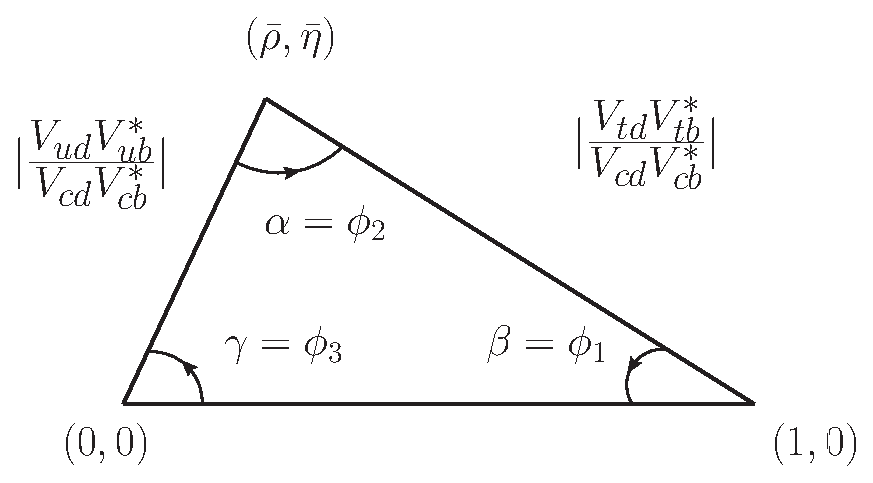
\includegraphics[width=0.5\textwidth]{theory/unitarity.eps}
\caption{Unitarity triangle in a complex plane.}
\label{fig:unitr}
\end{figure}
The area of the triangle is half of the Jarlskog invariant \textit{J}, a quantifier of CP violation, which is defined as $\rm{Im}[V_{ij}V_{kl}V^*_{il}V^*_{kj}]$ \cite{Jarlskog:1985ht}. It is interesting to notice that the \gls{SM} with its parameters may or may not violate CP. Only after measuring \textit{J} it is possible to determine the CP non-conservation. \textit{J} vanishes only if the mixing angle $\theta_{ij} = \{0 , \pi/2\}$; $\delta = \{0 , \pi\}$. So measurements of \textit{J} allows to verify that the \gls{CKM} matrix is complex and hence different mixing for quarks and anti-quarks is obtained.% although \gls{SM} CP violation is not big enough to explain the matter dominated universe.

The \gls{CKM} matrix elements which comprise of magnitudes and phases can be determined in different ways but the most precise option employs a global fit to all available measurements as shown in~\autoref{fig:unifit}. Hence, the most precise measurement of the \gls{CKM} matrix magnitudes to-date \cite{Patrignani:2016xqp} is 
%\begin{equation}|V_{\rm CKM}| = \begin{pmatrix}0.97446 \pm 0.00010 & 0.22452 \pm 0.00044  & \colorboxed{green}{0.00365\pm 0.00012} \cr
%	0.22438 \pm 0.00044 &  0.97359 \bfrac{+0.00010}{-0.00011} & 0.04214\pm 0.00076 \cr
%0.00896 \bfrac{+0.00024}{-0.00023} & 0.04133 \pm 0.00074 &  0.999105 \pm 0.000032 \cr \end{pmatrix},
%\end{equation}
\begin{equation}|V_{\rm CKM}| = \begin{pmatrix} 0.97434\bfrac{+0.00011}{-0.00012} & 0.22506 \pm 0.00050 & \colorboxed{green}{0.00357 \pm 0.00015}\cr
	0.22492 \pm 0.00050 &  0.97351 \pm 0.00013 & 0.0411 \pm 0.0013 \cr
0.00875 \bfrac{0.00032}{-0.00033} &  0.0403 \pm 0.0013 & 0.99915 \pm 0.00005  \cr \end{pmatrix},
\end{equation}
with non-zero Jarlskog invariant $J=(3.18\pm0.15)\times 10^{-5}$. Highlighted is the result for \DIFaddbegin \DIFadd{the }\DIFaddend magnitude of the $V_{ub}$ matrix element, $|V_{ub}|$, which is the element with \DIFaddbegin \DIFadd{the }\DIFaddend highest fractional uncertainty on its value. Therefore precise measurement of this element is very important and was the original motivation for the analysis of \Bmumumu. Moreover, as displayed in~\autoref{fig:unifit}(a)(b), the measurement of $|V_{ub}|$ (orange circle)(green circle) together with $\sin(2\beta)$ measurement (green band)(blue band) constrain the apex of the triangle. This means that these two measurements together with other measurements test the unitarity of the \gls{CKM} matrix, one of the fundamental assumptions of the \gls{SM}.


\begin{figure}[h]
\centering
%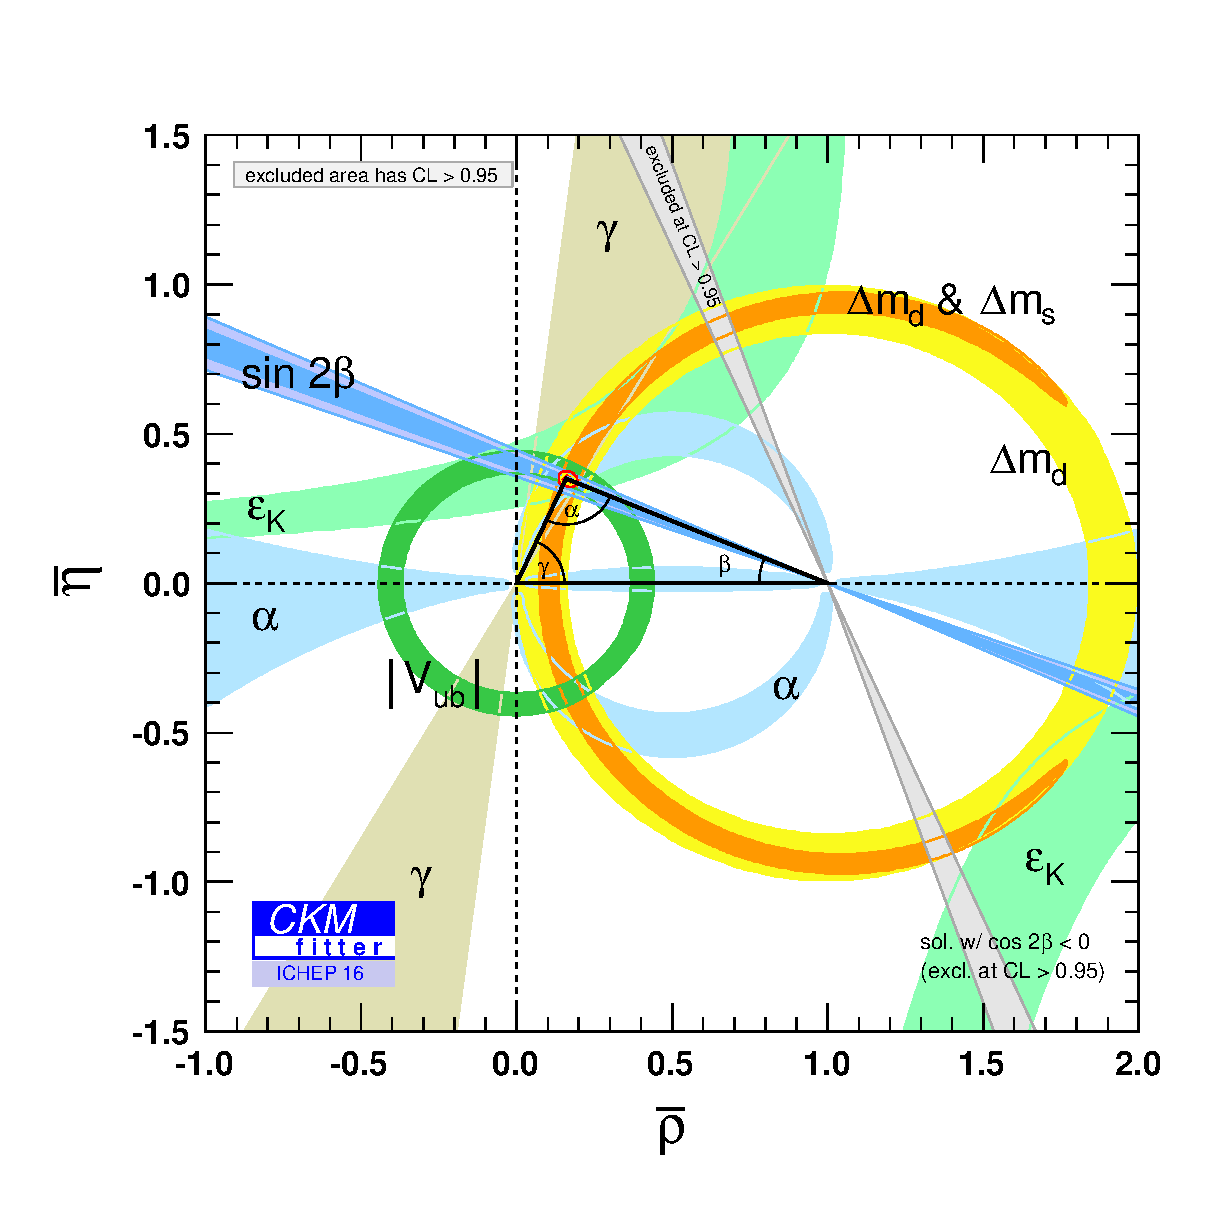
\includegraphics[width=0.7\textwidth]{theory/rhoeta_large_lol.eps}
\vspace*{-1.5cm}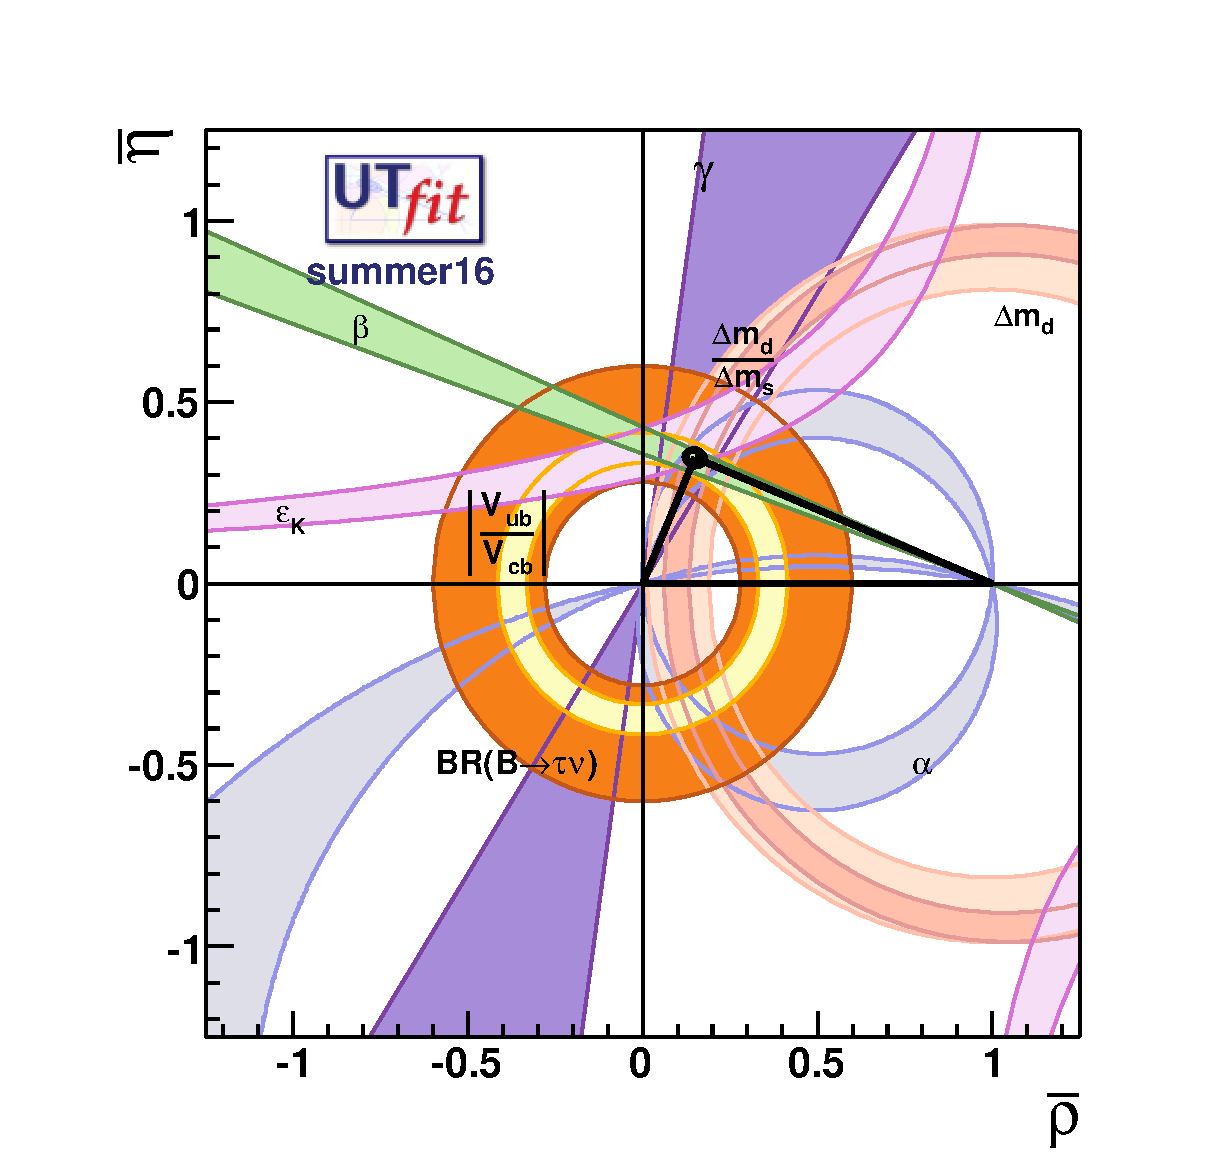
\includegraphics[width=0.65\textwidth]{theory/rhoeta-fullfit-sm.eps}\put(30,130){(a)}
\newline
\hspace*{-1.7cm}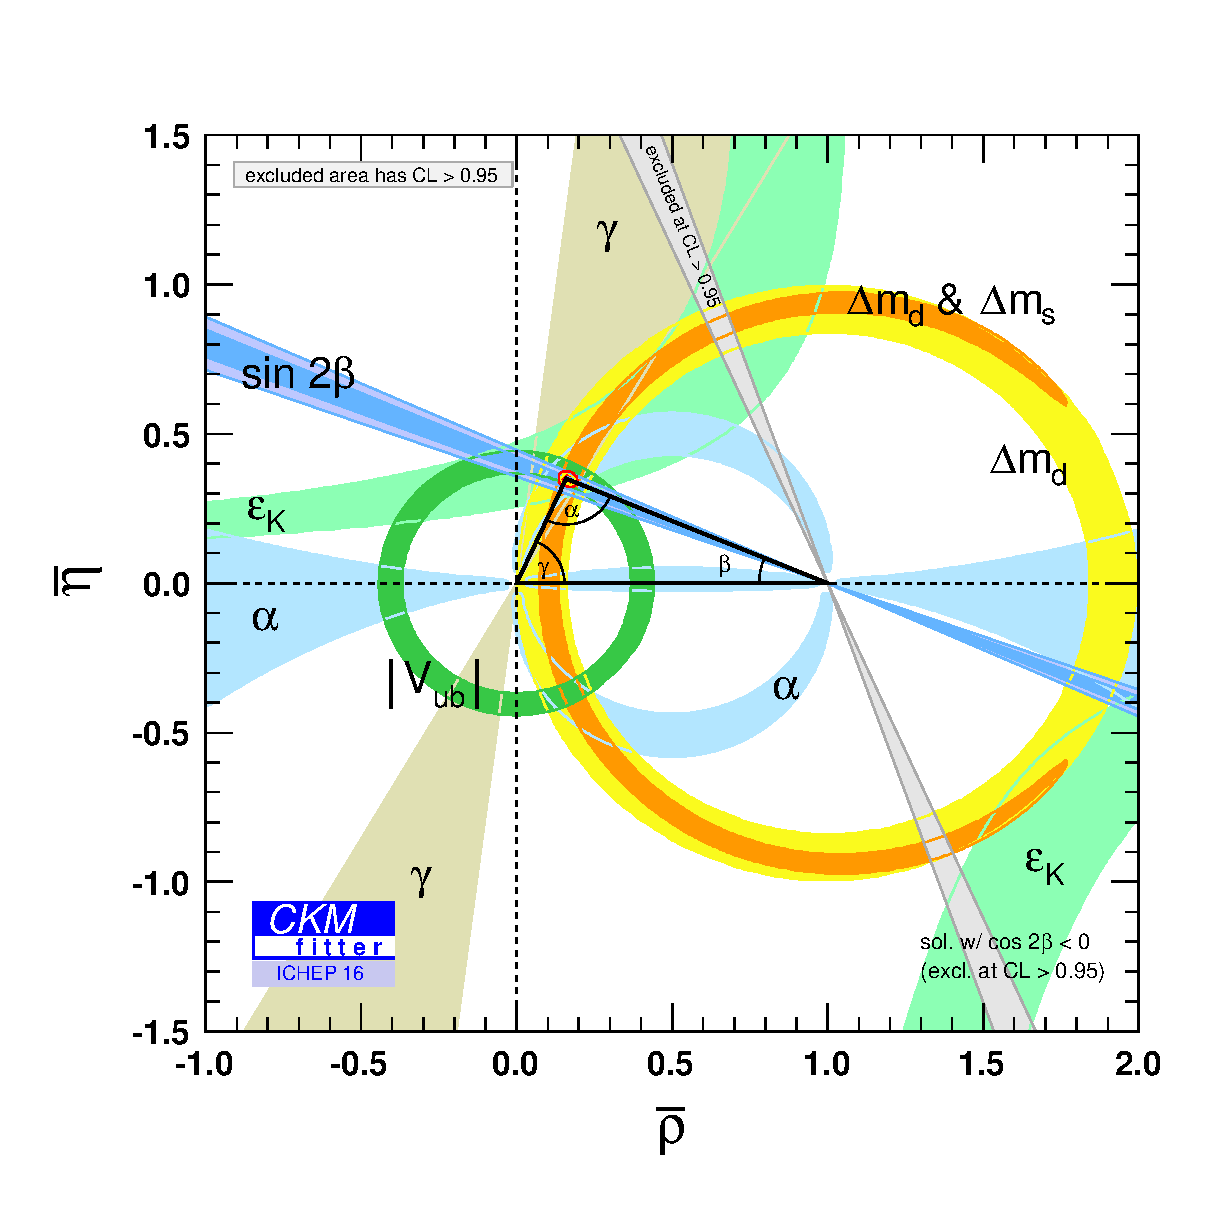
\includegraphics[width=0.65\textwidth]{theory/rhoeta_large_lol.eps}\put(30,130){(b)}
\caption{Different experimental measurements that constrain the \gls{CKM} matrix elements together with the global fit results from two collaborations (a) UTFit and (b) CKMFitter as of summer 2016. \DIFdelbeginFL \DIFdelFL{This }\DIFdelendFL \DIFaddbeginFL \DIFaddFL{These }\DIFaddendFL figures are taken from \DIFaddbeginFL \DIFaddFL{Refs.}\DIFaddendFL \cite{Bona:2006ah} and \cite{Charles:2004jd}. There is a good agreement for the results between the two different collaborations.}
\label{fig:unifit}
\end{figure}


\section{Fully Leptonic \mb{P^{+}\rightarrow l^{+} \nu} Decays}
\label{lnudecays}
%This text is based on a summary provided by PDG on Leptonic Decays of Charged Pseudoscalar Mesons.
Purely leptonic decays that proceed via annihilation-type diagrams of pseudoscalar mesons ($P$) are of great interest for flavour physicists because they allow \DIFaddbegin \DIFadd{one }\DIFaddend to make:
 \begin{itemize} 
\item either measurements of the \gls{CKM} matrix elements,
\item or measurements of leptonic decay constants,
\item or measurements of new physics effects.
 \end{itemize} 
The first two types of \DIFdelbegin \DIFdel{measurements }\DIFdelend \DIFaddbegin \DIFadd{measurement }\DIFaddend are possible because the decay rates of $P^{+}\rightarrow l^{+} \nu$ decays are sensitive to the product of the appropriate \gls{CKM} matrix element ($V_{q_{1}q_{2}}$ where $q_{1}$ and $q_{2}$ are \DIFaddbegin \DIFadd{the }\DIFaddend constituent quarks of the pseudoscalar meson) and decay constant $f_{P}$, \DIFaddbegin \DIFadd{a }\DIFaddend related parameter arising from the strong interaction. In more detail, the decay width of a fully leptonic decay of a pseudoscalar meson in the \gls{SM} to the lowest order can expressed as 

\begin{equation}
%\label{eqn:br} 
\Gamma(P^{+} \rightarrow {l^{+}} \nu)=  
	\frac{G_{F}^{2} m^{}_{P^{+}}  m_{l^{+}}^{2}}{8\pi} 
	\left[1 - \frac{m_{l^{+}}^{2}}{m_{P^{+}}^{2}}\right]^{2}  
	f_{P}^{2} |V_{q_{1}q_{2}}|^{2} 
	,
\label{eqn:dw} 
\end{equation}
where
$G_F$ is the Fermi constant,
$m^{}_{P^{+}}$ and $m_{l^{+}}$ are the pseudoscalar meson and lepton masses, respectively. This decay width can be compared to that of $\tau \rightarrow l\nu \bar{\nu}$\cite{Marciano:1988vm}


\begin{equation}
%\label{eqn:br} 
\Gamma(\tau \rightarrow {l} \nu \bar{\nu})=
	\DIFdelbegin \DIFdel{\frac{G^{2}_{l\tau} m^{5}_{\tau}}{192\pi^{3}}}\DIFdelend \DIFaddbegin \DIFadd{\frac{G^{2}_{F} m^{5}_{\tau}}{192\pi^{3}}}\DIFaddend \left[1-f\big(\DIFdelbegin \DIFdel{\frac{m^{2}_{l'}}{{m^{2}_{\tau}}}}\DIFdelend \DIFaddbegin \DIFadd{\frac{m^{2}_{l}}{{m^{2}_{\tau}}}}\DIFaddend \big)\right],
\label{eqn:tauonic} 
\end{equation}
\DIFdelbegin \DIFdel{where $G_{l\tau}$, is relevant Fermi constant. }\DIFdelend In this case $ f(x) = 1  8x - 8x^{3} + x^{4} + 12x^{2}\mathrm{log}(x)$ represents a correction due to the mass of the lepton
%(finite lepton mass)
in the final state. Corrections arising from the $W$ propagator effects are negligible for this decay and are not considered here and nor are radiative corrections so that only the lowest order contributions are considered. As compared to~\autoref{eqn:dw} the decay width is significantly higher. 

So in order to measure the \gls{CKM} matrix amplitude, knowledge of $f_{P}$ must be inferred. $f_{P}$ can be calculated using lattice \gls{QCD} techniques and together with experimental determination of the decay rates provide a way to determine the amplitude squared of the relevant \gls{CKM} matrix element assuming there is no contribution from new physics. More conventionally, \gls{CKM} magnitudes are determined from semileptonic decays, which \DIFdelbegin \DIFdel{is }\DIFdelend \DIFaddbegin \DIFadd{are }\DIFaddend experimentally 
more accessible but \DIFdelbegin \DIFdel{entails }\DIFdelend \DIFaddbegin \DIFadd{entail }\DIFaddend larger theoretical uncertainty.
%\gls{CKM} magnitudes are determined from semileptonic decays different type of current is given \mybox{this is in pdg i dont understand why is it wrong}. In purely leptonic decays axial-vector flavour-changing currents ($q_{1}\gamma_{\mu}\gamma_{5}q_{2}$) are probed as opposed to vector current ($q_{1}\gamma_{\mu}q_{2}$) in semileptonic case.

Vice versa, assuming unitarity of \DIFaddbegin \DIFadd{the }\DIFaddend \gls{CKM} triangle and experimental determination of \DIFaddbegin \DIFadd{the }\DIFaddend relevant $V_{q_{1}q_{2}}$ one can obtain experimental determination of the decay constants and compare it with theoretical prediction.

Last, but not least, is of course the measurement of presence of new physics in these decays. Especially appealing is the presence of new particles which would manifest themselves in the decay rates of heavier pseudoscalars ($D_{(s)}$ or $B$). \DIFdelbegin \DIFdel{An example }\DIFdelend \DIFaddbegin \DIFadd{Example }\DIFaddend of such new particles \DIFdelbegin \DIFdel{include }\DIFdelend \DIFaddbegin \DIFadd{are }\DIFaddend charged Higgs bosons, $H^{\pm}$, coming from so-called Type II Higgs-doublet models \cite{Hou:1992sy}\cite{Akeroyd:2003zr}\cite{Dobrescu:2008er} or leptoquarks\cite{Dobrescu:2008er}. In this case, considering $B^{+}\rightarrow l^{+}\nu$ decay, the four-fermion interaction between \DIFaddbegin \DIFadd{the }\DIFaddend $W^{\pm}$ and $H^{\pm}$ \DIFaddbegin \DIFadd{bosons }\DIFaddend would modify the \gls{SM} decay width~\autoref{eqn:dw} to
%remember branching fraction is partial width of total width
%total width  h over liftime so lifetime is always missing from equations 
% see https://www2.ph.ed.ac.uk/~vjm/Lectures/ParticlePhysics2010_files/Particle3-2Nov.pdf this

\begin{equation}
\Gamma(B^{+} \rightarrow {l^{+}} \nu)=  
        \frac{G_{F}^{2} m^{}_{B^{+}}  m_{l^{+}}^{2}}{8\pi} 
        \left[1 - \frac{m_{l^{+}}^{2}}{m_{B^{+}}^{2}}\right]^{2}  
	f_{P}^{2} |V_{ub}|^{2} \,\times\, r_H,
%\Gamma(B^+\to \ell^+\nu_\ell)={G_F^2 m_{B} m_l^2 f_{B}^2\over 8\pi}
%|V_{ub}|^2 \left(1-{m_l^2\over m^2_{B}}\right)^2 \,\times\, r_H
\end{equation}
where
\begin{equation}
	r_H=[1-\tan^2\beta(m^{2}_{B^{+}}/m^{2}_{H^{+}})]^2.
\end{equation}
Here $\tan\beta = \frac{v_{2}}{v_{1}}$, where $v_{i}$ are the vacuum expectation values for the Higgs doublets. In order to have an enhancing effect for the rate of the $B^{+}\rightarrow l^{+}\nu$ decay (to have $r_{H}>1$), $\tan\beta/m_{H^{\pm}}> 0.27 \gev^{-1}$. The experimental limit presents already a strong lower bound on the charged Higgs mass $m_{H^{\pm}}>600\gev$\cite{Arbey:2017gmh}. This makes the most of the parameter space in $\tan\beta$ and $m_{H^{\pm}}$ satisfy enhancing condition of $\tan\beta/m_{H^{\pm}}>0.27 \gev^{-1}$.

The ratio of rates between $P\rightarrow\tau\nu$, $P\rightarrow\mu\nu$ and $P\rightarrow e\nu$ decays could also be of an interest. In the ratios the decay constant $f_{P}$ cancels out making such measurements a good tool for lepton universality tests.

As seen in~\autoref{eqn:dw}, a purely leptonic final state going through $P\rightarrow W^{*}\rightarrow l \nu$ is suppressed by $\frac{m^{2}_{l}}{m^{2}_{p}}$, also known as helicity suppression. This suppression occurs as a result of angular momentum conservation. In case of $B^{+}\rightarrow l^{+} \nu$, the $B^{+}$ is a spin-0 particle and hence its decay products should have spin 0 combined, or in other words, be anti-aligned. Neutrinos in the \gls{SM} are always produced left-handed. As the spin of the antilepton and the neutrino should be anti-aligned, the antilepton also needs to be left-handed (to have negative helicity). However, the weak current only couples to right-handed antiparticles. Therefore, the antilepton has to be boosted in order to have different helicity. For massless particles such a helicity flip is not possible making this decay impossible. The lighter the lepton, the larger the velocity and hence higher boost is necessary, making decays to lighter leptons rarer even though they have bigger kinematic phase space available.

%https://www.physicsforums.com/threads/helicity-and-suppression.804600/
Concentrating on the decays $B^{\pm}$ meson, the latest experimental measurements for rates of $B^{+}\rightarrow l^{+} \nu$ decays have been performed by $B$ factories, finding evidence for $B^{+}\rightarrow \tau^{+}\nu$ and first sign of $B^{+}\rightarrow \mu^{+}\nu$ as seen in~\autoref{tab:sum}. These results are to be compared with the \gls{SM} predictions $\mathcal{B}(B^{+}\rightarrow \tau^{+}\nu) = (0.82+0.03-0.02)\times10^{-4}$\cite{Charles:2004jd} and $\mathcal{B}(B^{+}\rightarrow \mu^{+}\nu) = (3.80\pm0.31)\times10^{-7}$\cite{Sibidanov:2017vph}, which are obtained by using $|V_{ub}|$ value resulting from other measurements and lattice calculations of $f_{B}$. %Quite substantial statistical as well as systematical errors show the difficulty of this type of measurements. 



\begin{table}[ht]
\begin{center}
\begin{tabular}{ l l l l H c H} \toprule
        Process &Experiment & Tag &${\mathcal{B}}$ & Published & Significance & {$|V_{ub}|f_{B^+}$ (MeV)} \hfill\\
	 & &  & & & [$\sigma$] & {$|V_{ub}|f_{B^+}$ (MeV)} \hfill\\
\hline\\[-2.5ex]
        $B^{+}\rightarrow \tau^{+}\nu$  &Belle~\cite{Adachi:2012mm}&Hadronic&$(0.72^{+0.27}_{-0.25}\pm0.11)\times10^{-4}$  & 2013 & 3.0 \\
        $B^{+}\rightarrow \tau^{+}\nu$  &Belle~\cite{Kronenbitter:2015kls}&Semileptonic&$(1.25\pm0.28\pm0.27)\times10^{-4}$ & 2015 & 3.8 \\
        $B^{+}\rightarrow \tau^{+}\nu$  &Belle~\cite{Kronenbitter:2015kls}&Average&$(0.91 \pm 0.22)\times10^{-4}$ & 2015 & 4.6 \\\hline\\[-2.5ex]
        $B^{+}\rightarrow \tau^{+}\nu$  &BaBar~\cite{Lees:2012ju} & Hadronic & $(1.83\,^{+0.53}_{-0.49}\pm0.24)\times10^{-4}$ & 2012 & 3.8 \\
        $B^{+}\rightarrow \tau^{+}\nu$  &BaBar~\cite{Aubert:2009wt} & Semileptonic & $(1.7\pm 0.8\pm 0.2)\times10^{-4}$ & 2010 & 2.3\\
        $B^{+}\rightarrow \tau^{+}\nu$  &BaBar~\cite{Lees:2012ju} & Average & $(1.79 \pm 0.48)\times 10^{-4}$ & 2012 & - & $1.01\pm 0.14$  \\ \hline
$B^{+}\rightarrow \mu^{+}\nu$ & Belle~\cite{Sibidanov:2017vph} & Untagged& $(6.46\pm2.22\pm 1.60)\times 10^{-7}$ & 2017 & 2.4 &\\
%        & Our average & &$1.06\pm0.20$&$0.77\pm0.07$ & & \\
\bottomrule
\end{tabular}
\end{center}
\caption{Experimental summary of searches for $B^{+}\rightarrow l^{+}\nu$ that is inspired from \cite{Patrignani:2016xqp}. Tag Hadronic/Semileptonic/Untagged refers to different way data is selected in Belle and BaBar factories.}
\label{tab:sum}
\end{table}




With helicity suppressed rates and very limited signatures in the detector (one charged track for muons and electron, more charged tracks for taus, but also more missing energy depending on the reconstruction channel) searching for such decays is very challenging. In order to make measurements of the same kind (CKM precision measurements, decay constants measurements, new physics searches), fully leptonic decays with photons can be considered.   

\section{Fully Leptonic \mb{B^{+}\rightarrow l^{+} \nu \gamma} Decays}
\label{lnugamma}
The helicity suppression of $B^{+}\rightarrow l^{+} \nu$ decays can be lifted by considering the decay with an additional photon radiated from the $B^{+}$ meson, at the cost of the electromagnetic suppression with coupling constant $\alpha_{em}$. Consequently, the branching fraction for radiative decays can be comparable or even larger than the corresponding fraction for purely leptonic decays. It has been shown that $R^{\mu}_{B}=\frac{\Gamma(B\rightarrow \mu \nu \gamma)}{\Gamma(B\rightarrow \mu \nu)}\approx(1-20)$ making $\mathcal{B}(B\rightarrow \mu \nu \gamma)\approx(10^{-7}-10^{-6})$ \cite{Burdman:1994ip}.

%As compared to photonless decays, the amplitude of the decay will have a contribution from both the axial-vector weak current as well as the vector current.
The differential decay width with $\frac{1}{m_{b}}$ and radiative corrections
at next-to-leading logarithmic order calculated in\cite{Beneke:2011nf} is given by
\begin{equation}
\frac{d\Gamma}{dE_{\gamma}} = \frac{\alpha_{em}G^{2}_{F}|V_{ub}|^{2}}{48 \pi^{2}}m_{B}^{4}(1 - x_{\gamma})x_{\gamma}^{3}[F_A^{2} + F_V^{2}],
\end{equation}
 where $x_{\gamma} = 2E_{\gamma}/m_{B}$, $F_A$ is the axial form factor and $F_V$  is the vector form factor defined as
\begin{equation}
F_{V}(E_{\gamma}) = \frac{Q_{u}m_{B}f_{B}}{2E_{\gamma}\lambda_{B}(\mu)} R(E_{\gamma}, \mu) + [\xi(E_\gamma) +  \frac{Q_{u}m_{B}f_{B}}{(2E_{\gamma})^{2}} + \frac{Q_{b}m_{B}f_{B}}{2E_{\gamma}m_{b}}],
\label{eq:top1}
\end{equation}

\begin{equation}
F_{A}(E_{\gamma}) = \frac{Q_{u}m_{B}f_{B}}{2E_{\gamma}\lambda_{B}(\mu)} R(E_{\gamma}, \mu) + [\xi(E_\gamma) -  \frac{Q_{u}m_{B}f_{B}}{(2E_{\gamma})^{2}} - \frac{Q_{b}m_{B}f_{B}}{2E_{\gamma}m_{b}} + \frac{Q_{l}f_{B}}{E_{\gamma}}].
\label{eq:top2}
\end{equation}
Here $Q_{l},Q_{u},Q_{b}$ are the charges of the lepton, up quark, and
bottom quark, respectively, and $R(E_{\gamma}, \mu)$ is a radiative correction
calculated at the energy scale $\mu$ %that equals one at tree level.
and $m_{b}$ is the mass of the $b$ quark.

The first term in~\autoref{eq:top1} and ~\autoref{eq:top2} represents the leading-power contribution in the heavy-quark expansion. Note that this term
is the same for the vector and axial form factor. The second terms are $\frac{1}{m_{b}}$ power corrections relative to the leading term. Further corrections have been discussed in~\cite{Wang:2016beq}.



Recent measurement of the radiative $B^{+} \rightarrow l^{+} \nu \gamma$, where $l^{+}$ is either $e^{+}$ or $\mu^{+}$ was performed by Belle using hadronic tagging on their full data sample\cite{Heller:2015vvm}. The search yielded $\mathcal{B}(B^{+}\rightarrow \mu^{+} \nu \gamma) < 3.4\times 10^{-6}$ and $\mathcal{B}(B^{+}\rightarrow e^{+} \nu \gamma) < 6.1\times 10^{-6}$.



\section{Fully Leptonic \mb{B^{+}\rightarrow l^{+} l^{-} l^{+} \nu} Decays}
\label{mydecay}

In LHCb, the most optimal approach due to the detector capabilities is to measure this kind of decay by converting the photon into a pair of muons, see~\autoref{fig:myfeyn}(a). If the naive expectation of only taking into account photon conversion into two muons is adopted, then the expected branching fraction for this analysis is $\mathcal{B}(B^{+}\rightarrow \mu^{+} \mu^{-} \mu^{+} \nu) \approx 1.0\times 10^{-8}$. However, such estimate is not correct because there are other contributions to the total decay rate as shown in the first theoretical prediction for $\mathcal{B}(B^{+}\rightarrow \mu^{+} \mu^{-} \mu^{+} \nu)$ in \cite{Danilina:2018uzr} based on the Vector Meson Dominance (VMD) model. This theoretical prediction yields $\mathcal{B}(B^{+} \rightarrow \mu^{+} \mu^{-} \mu^{+} \nu) \approx 1.3\times 10^{-7}$.% and the rest of this section is a short summary of this publication.

 The VMD model was formulated to describe the interaction between photons and hadrons before \gls{QCD} was formulated. It is an approximative model where the photon is treated to be made of a purely electromagnetic component and a vector meson component. This idea originates in the fact that both photon and vector mesons have the same quantum numbers $J^{PC} = 1^{-\ -}$ and if two particles have the same quantum numbers then they mix. %(the state which commutes with the Hamiltonian is a superposition of all such states). 
% Therefore, there is mixing between photons and vector mesons.

As mentioned previously, there are different contributions to the amplitude of the $\mathcal{B}(B^{+}\rightarrow \mu^{+} \mu^{-} \mu^{+} \nu)$. Using the VMD model, it is not surprising that the biggest contribution arises from the photon emission from the valence $u$-quark of the $B$ meson. In this case, the contribution from the $\rho(770)$ and $\omega(782)$ resonances are included in the calculation. Secondly, the contribution of photon emission from the $b$-quark is studied, effectively creating excited $B^{+}$, $B^{+*}$ intermediate resonance state. Thirdly, the photon can be emitted from the final-state lepton, a process known as Bremsstrahlung. All these different contributions to the decay amplitude are shown in~\autoref{fig:myfeyn}. To obtain the total amplitude, the sum of the matrix elements of the three contributions is calculated in the limit where $m_{l}$ is set to zero.


\begin{figure}[ht]
\centering
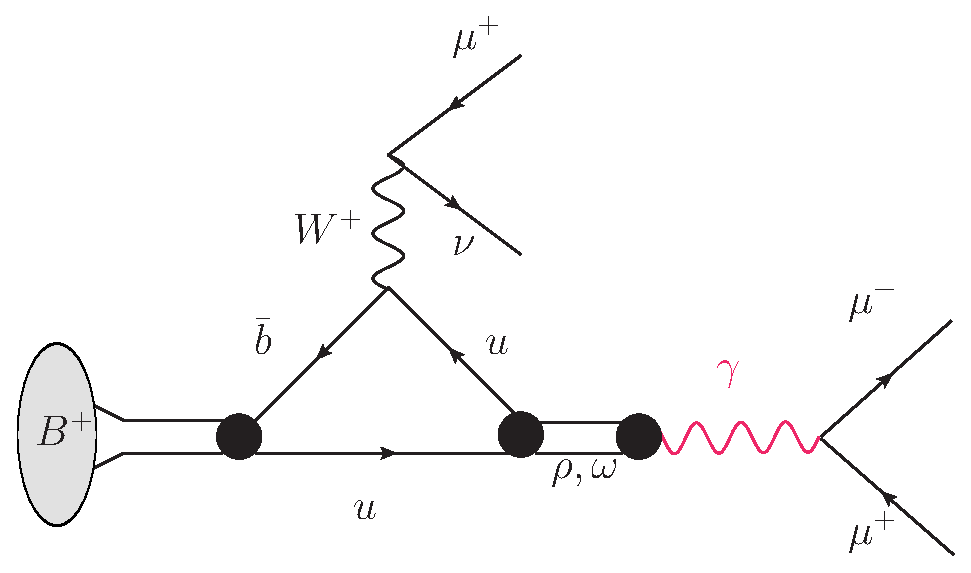
\includegraphics[scale=0.5]{theory/nik_1figure}\put(-30,133){(a)}
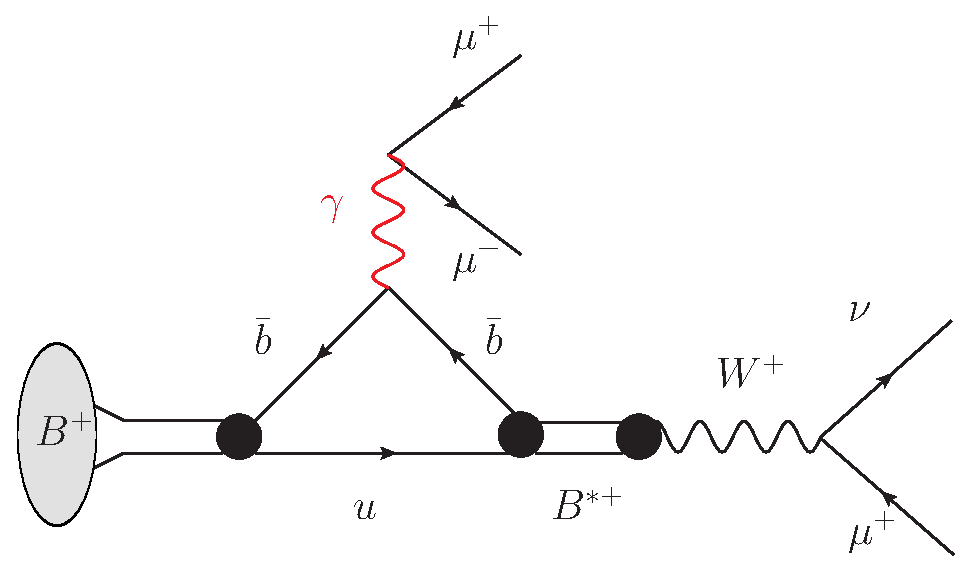
\includegraphics[scale=0.5]{theory/nik_2figure}\put(-30,133){(b)}
\newline
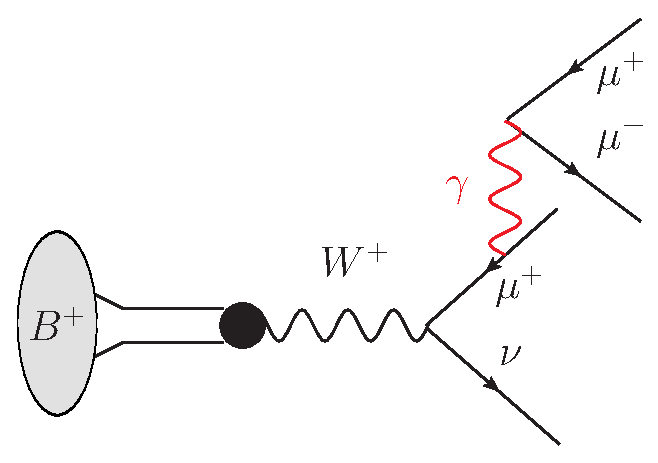
\includegraphics[scale=0.55]{theory/nik_3figure}\put(-30,133){(c)}
\centering
	\caption{Different contributions to the \Bmumumu decay. (a) Initial $u$-quark state radiates off a virtual photon which decays into a pair of muons and the $W^{+}$ decays into a muon and muon neutrino. Most of the contribution to the rate comes from hadronic contribution to the photon. (b) Photon emission from $b$-quark and (c) finally emission from the final state muon.}
\label{fig:myfeyn}
\end{figure}


In this publication the amplitude of $\mathcal{B}(B^{+}\rightarrow \mu^{+} \mu^{-} \mu^{+} \nu)$ is estimated by calculating $\mathcal{B}(B^{+}\rightarrow \mu^{+} \mu^{-} e^{+} \nu)$ amplitude first and then adding a negative interference term that arises due to the identical fermions in the final state doubling the number of possible diagrams. The numerical calculation yields $\mathcal{B}(B^{+}\rightarrow \mu^{+} \mu^{-} e^{+} \nu) \approx 1.3 \times 10^{-7}$ and $\mathcal{B}(B^{+}\rightarrow \mu^{+} \mu^{-} \mu^{+} \nu) \approx 1.3 \times 10^{-7}$. 

\section{The \mb{\Bmumumu} Decay Model}
\label{simulation}
As the search for the \Bmumumu decay is the first of its kind, a simulation that describes this type of decay was not available. There are, however, three types of decay models for \Bmumumu which were adopted and used for different purpose. More detail about their use is covered in~\autoref{SimulationSamples}.

For any decay, it is possible to use a phase space model, \textit{PHSP}, which only takes into account the kinematic constraints of the decay without taking into account any input from theoretical considerations as the matrix element is constant. This is not satisfactory for decays where there are intermediate virtual photons or vector meson resonances.

The following decay model is developed to reflect the expected behaviour of decays shown in~\autoref{fig:myfeyn}. The decay proceeds through a virtual $W$ decaying to $\mu^{+} \nu$ and a virtual photon decaying to a muon pair. This has similar structure to $\B^{+} \rightarrow (K^{*+}) \mu^{+} \mu^{-}$ decay, where the $K^{*+}$ can take the role of the virtual $W$ decay. By using the \textit{BTOSLLBALL} model\cite{Ali:1999mm}, traditionally used for $B^{+} \rightarrow (K^{*+}) l^{+} l^{-}$ decays, but modifying the properties of the $K^{*+}$ to those of virtual $W$ (having mass of 0.1 \gevcc and width 50 \gev), it is possible to obtain a good approximation to the correct features of the decay. This is visible in~\autoref{fig:mcgeneration}, where there is a characteristic photon pole for low $q(\mu^{+},\mu^{-})$, invariant mass of the opposite muon pair, and flat distribution for $K^{*}(\mu^{+}, \nu) $, invariant mass of the muon and neutrino pair. This decay model will be further referred to as \textit{INSP} model. 



%\mybox{Sally: move it to theory and check ulrik's comment} In order to produce simulation with a decay model which is more representative of the spin structure involved, the following strategy is adapted. In this simulation approach, the decay proceeds as follows: \Bpm decays into \Wpm and a pair of opposite sign muons and then \Wp is decayed to $\mu^{+} \nu$. \textit{BTOSLLBALL} model\cite{Ali:1999mm}, traditionally used for $\B \rightarrow (K,K^{*}) l^{+} l^{-}$ decay, with the form factor calculations can be used to simulate $\Bpm \rightarrow \Wpm l^{+} l^{-}$ decay. After that, \Wp is decayed to $\mu^{+} \nu$ using \textit{PHSP}. For semileptonic $b \rightarrow s l^{+} l^{-}$ transitions, there is a characteristic photon pole for low $q(\mu^{+},\mu^{-})$, invariant mass of the opposite muon pair, and flat distribution for $K^{*}(\mu^{+}, \nu) $, invariant mass of the muon and neutrino pair. In order to achieve this, a new pseudo-particle is introduced to EVTGEN with specific properties, $K^{*}(\mu^{+}, \nu)$, and the best output can be seen to be for a particle $K^{*}(\mu^{+}, \nu)$ with mass to be set to $0.1 \text{GeV/c}^{2}$, and width, corresponding to $\tau= 1.3\times10^{-17}$ nanoseconds as can be seen in~\autoref{fig:mcgeneration}. This procedure was also applied for the charge conjugate case. This model is denoted as \textit{INSP} and is used as default in mass fits and efficiency calculations.

\begin{figure}[h!]
\centering
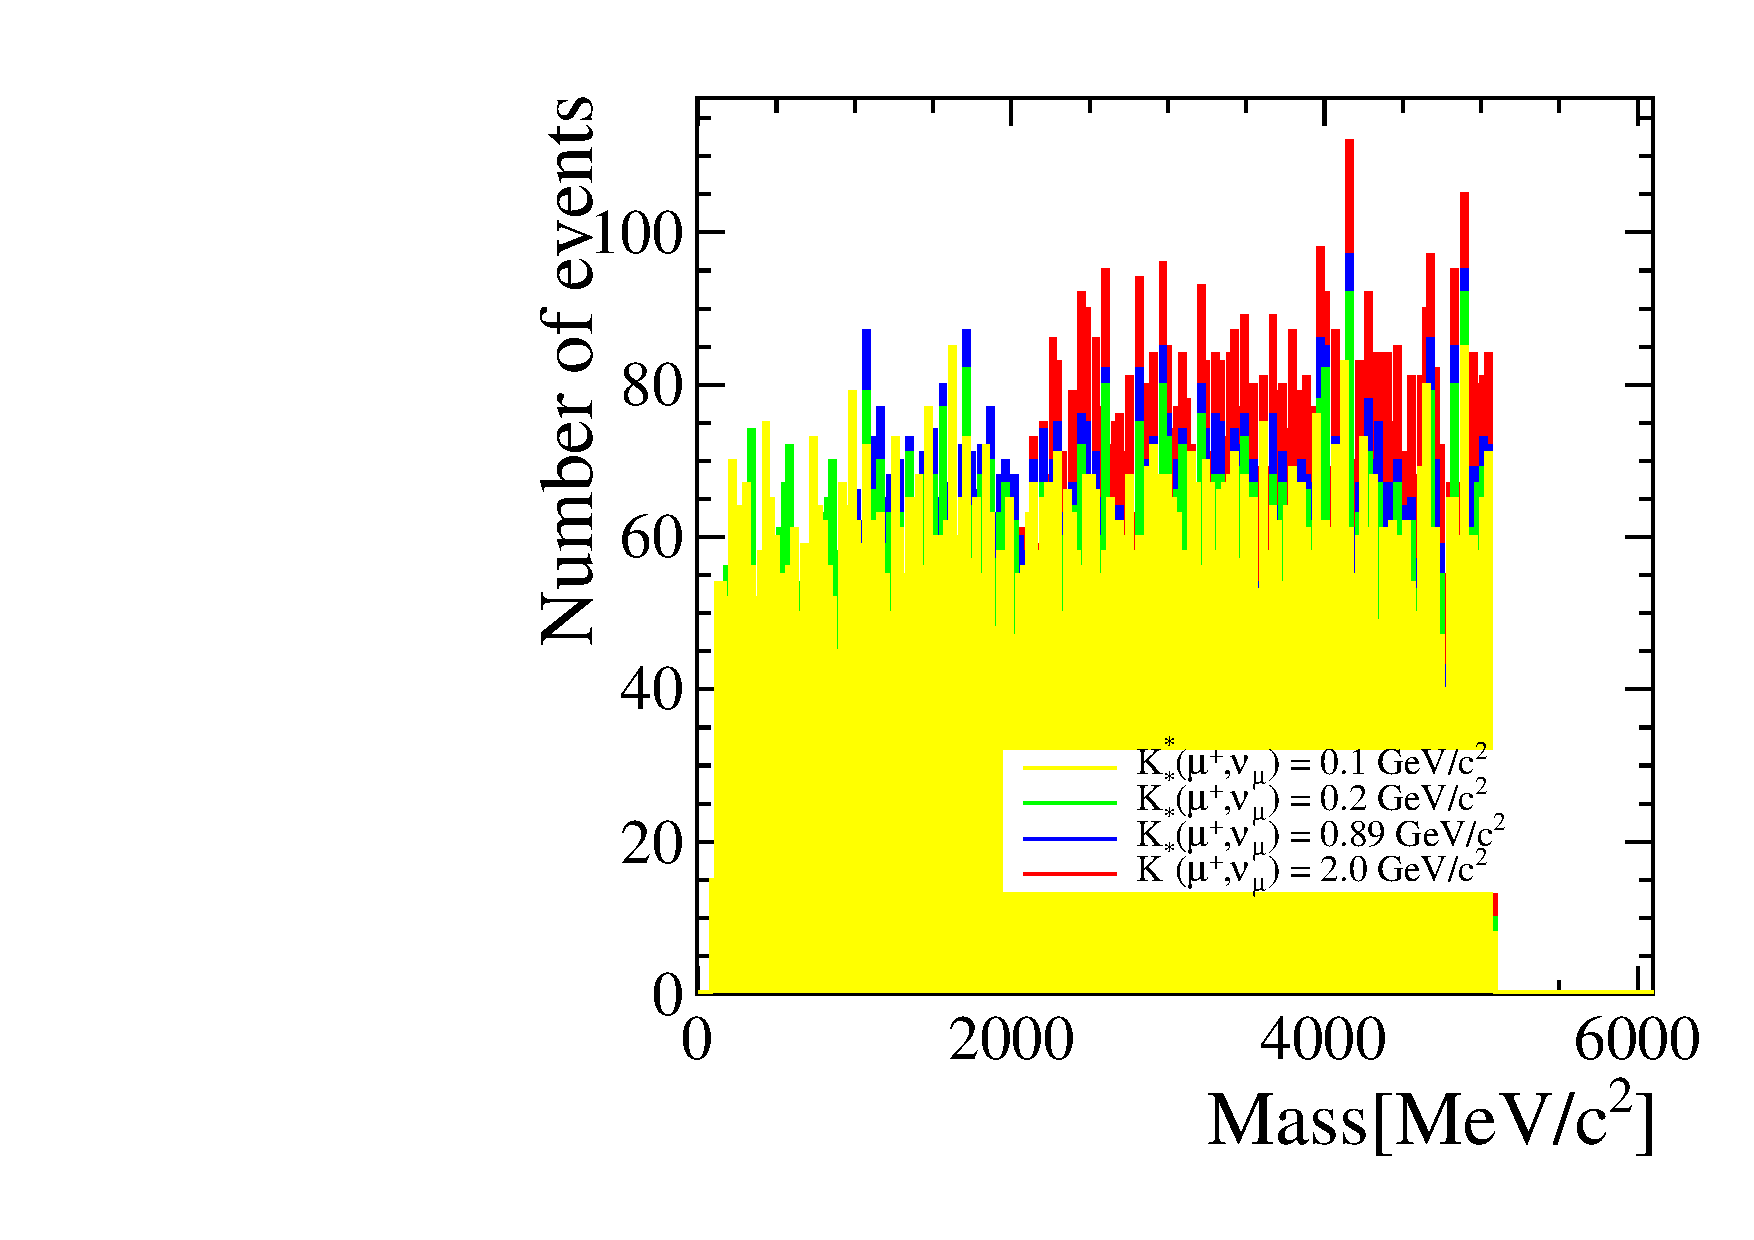
\includegraphics[width=0.5\linewidth]{./sel/reporttry_new}\put(-70,133){(a)}
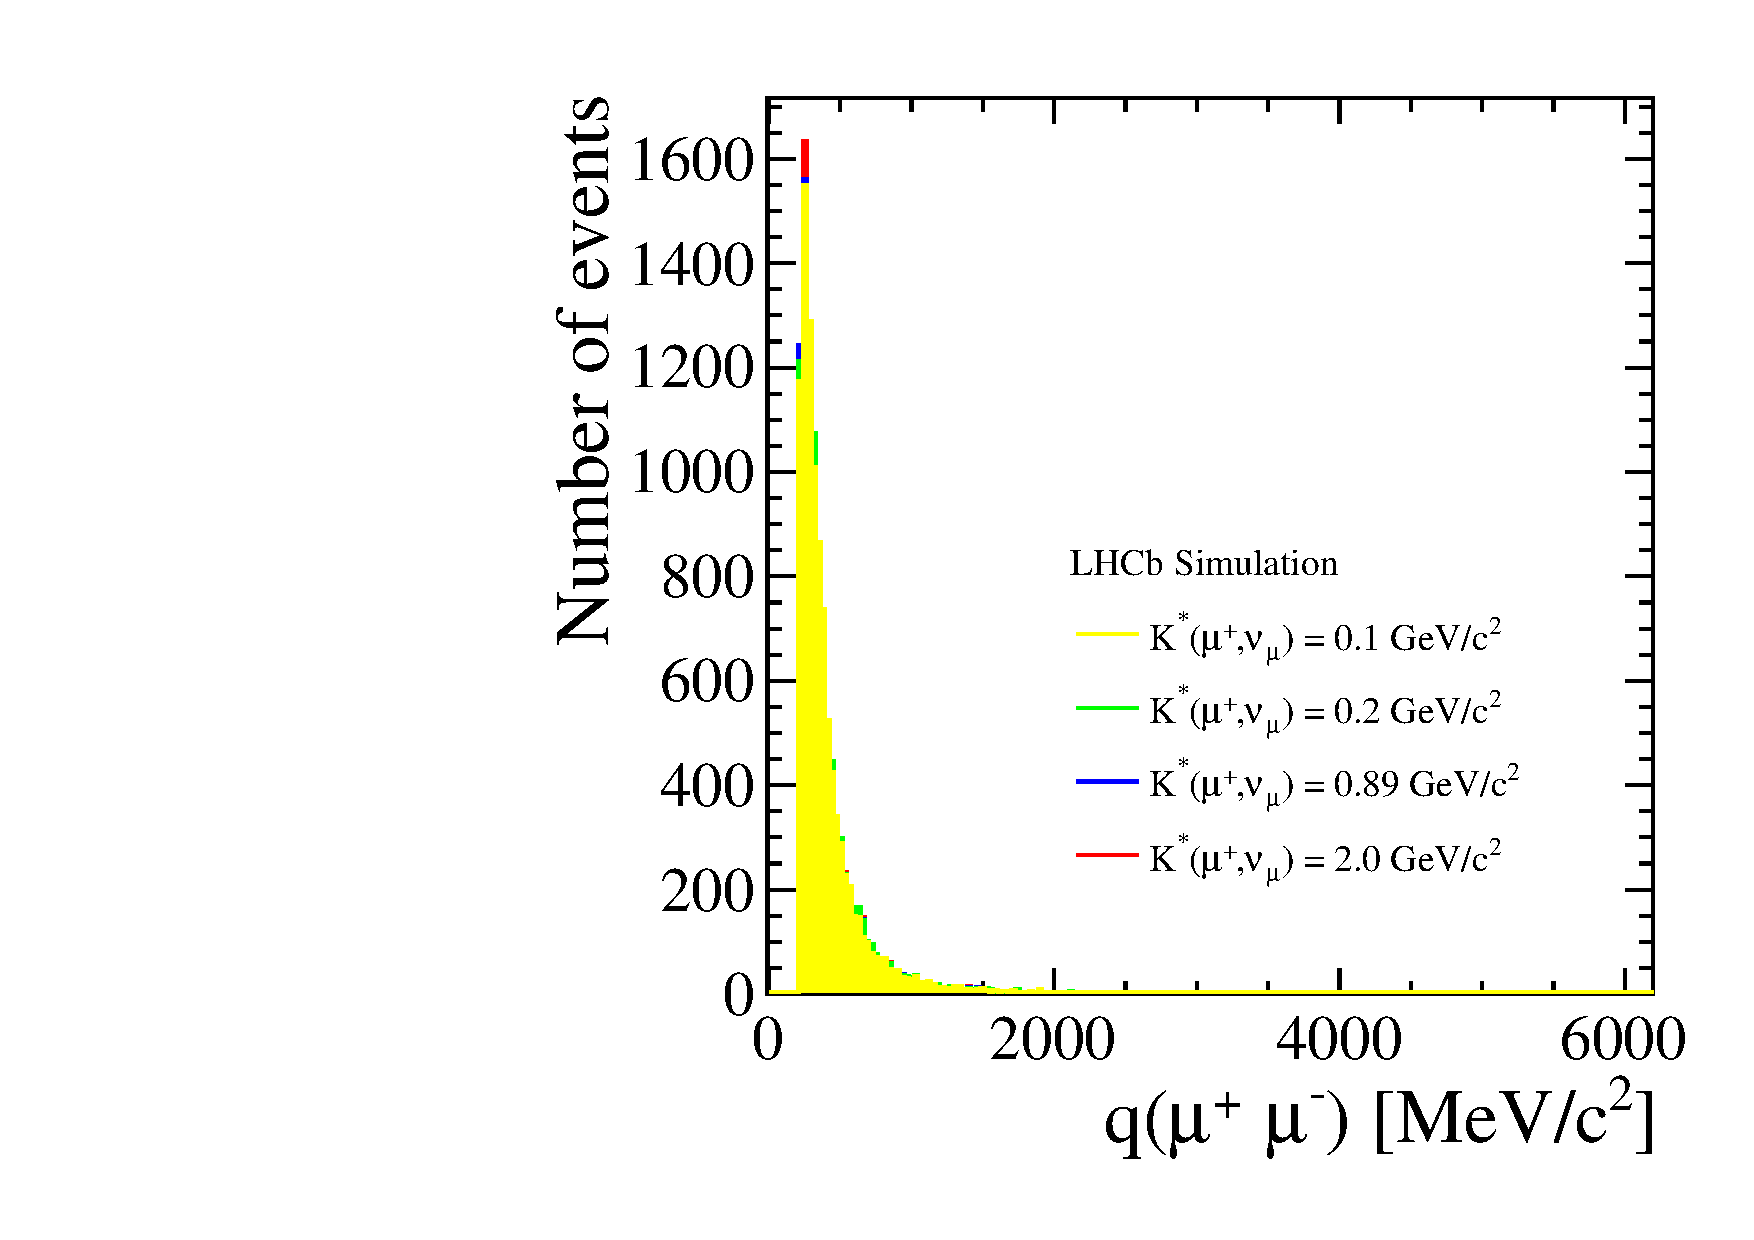
\includegraphics[width=0.5\linewidth]{./sel/reporttrialqpres_new}\put(-50,133){(b)}
\caption{Distributions for signal simulation. (a) $K^{*}(\mu^{+}, \nu)$ (b) $q(\mu^{+},\mu^{-})$ distributions under different $K^{*}$ mass hypotheses. The most flat distribution in $K^{*}(\mu^{+}, \nu)$ is plotted in yellow.}
\label{fig:mcgeneration}
%\vspace*{-1.0cm}
\end{figure}

Finally, there is a decay model based on calculations from VMD model, which was written by authors of \cite{Danilina:2018uzr}. This model denoted as \textit{NIKI}.


\chapter{The LHCb Detector}
\label{chap:dec}

\textit{In this section, an overview of the accelerator complex at CERN as well as the physics motivation behind the \Gls{LHCb} detector and its design will be described.}

CERN has built one of the most exciting laboratories to study elementary particle interactions in the world. Its complex set of particle accelerators and detectors is shown in~\autoref{fig:AcceleratorComplex}. The process of accelerating protons starts with the source of protons. Protons are obtained from a hydrogen gas bottle by applying an electric field separating hydrogen into protons and electrons. The first proton accelerator in the chain, Linac 2, accelerates the protons to the energy of 50 \mev. Linac 2 is a tank composed of several chambers where the resonant cavities are tuned to a specific frequency creating potential differences in them, which then make the protons accelerate. The protons are then injected into the Proton Synchrotron Booster (\Gls{PSB}), where they are accelerated further to 1.4 \gev. The next in line is the Proton Synchrotron (\Gls{PS}) reaching \DIFaddbegin \DIFadd{an }\DIFaddend energy of 25 \gev. Before either entering the Large Hadron Collider (\Gls{LHC}) or North Area (mainly used as testing facility for experiment upgrades) the Super Proton Synchrotron (\Gls{SPS}) is the last accelerator in the chain. Here proton acceleration to 450 \gev is achieved.

\begin{figure}
  \centering
  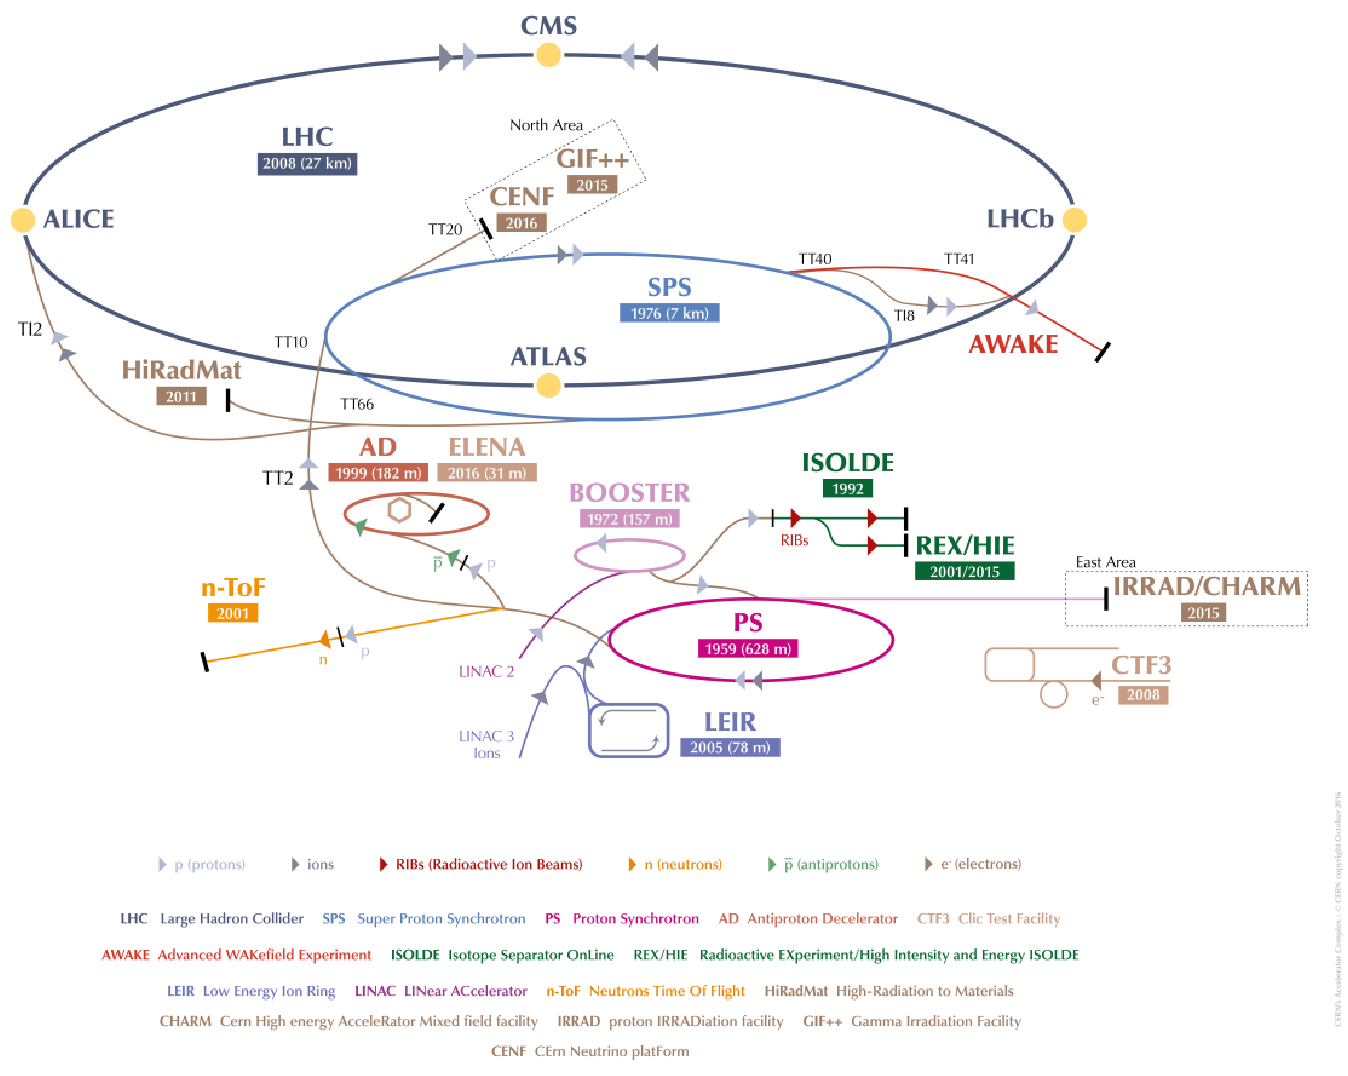
\includegraphics[width=1.0\linewidth]{figs/detector/AccComplexpng2pdf_cropped.pdf}
	\caption{Accelerator complex at CERN. The image is taken from \cite{complex}.}
  \label{fig:AcceleratorComplex}
\end{figure}

\DIFaddbegin \DIFadd{The }\DIFaddend \Gls{LHC} is a complex machine which accelerates beams of protons in opposite directions in a $\sim$ 27km long circular tunnel. It is located
50-157\m below ground crossing the border between Switzerland and France. Once the desired energy is achieved proton-proton ($pp$) or ion collisions happen at four distinct points, where different detectors with different physics focus are located. These are \Gls{ATLAS}, \Gls{CMS}, \Gls{ALICE} and \Gls{LHCb}. 
The search for the decay \Bmumumu was performed using data obtained at \Gls{LHCb}\DIFaddbegin \DIFadd{\mbox{%DIFAUXCMD
\cite{det_paper}}%DIFAUXCMD
}\DIFaddend . 

\section{LHCb Layout }

\begin{figure}
	\centering
	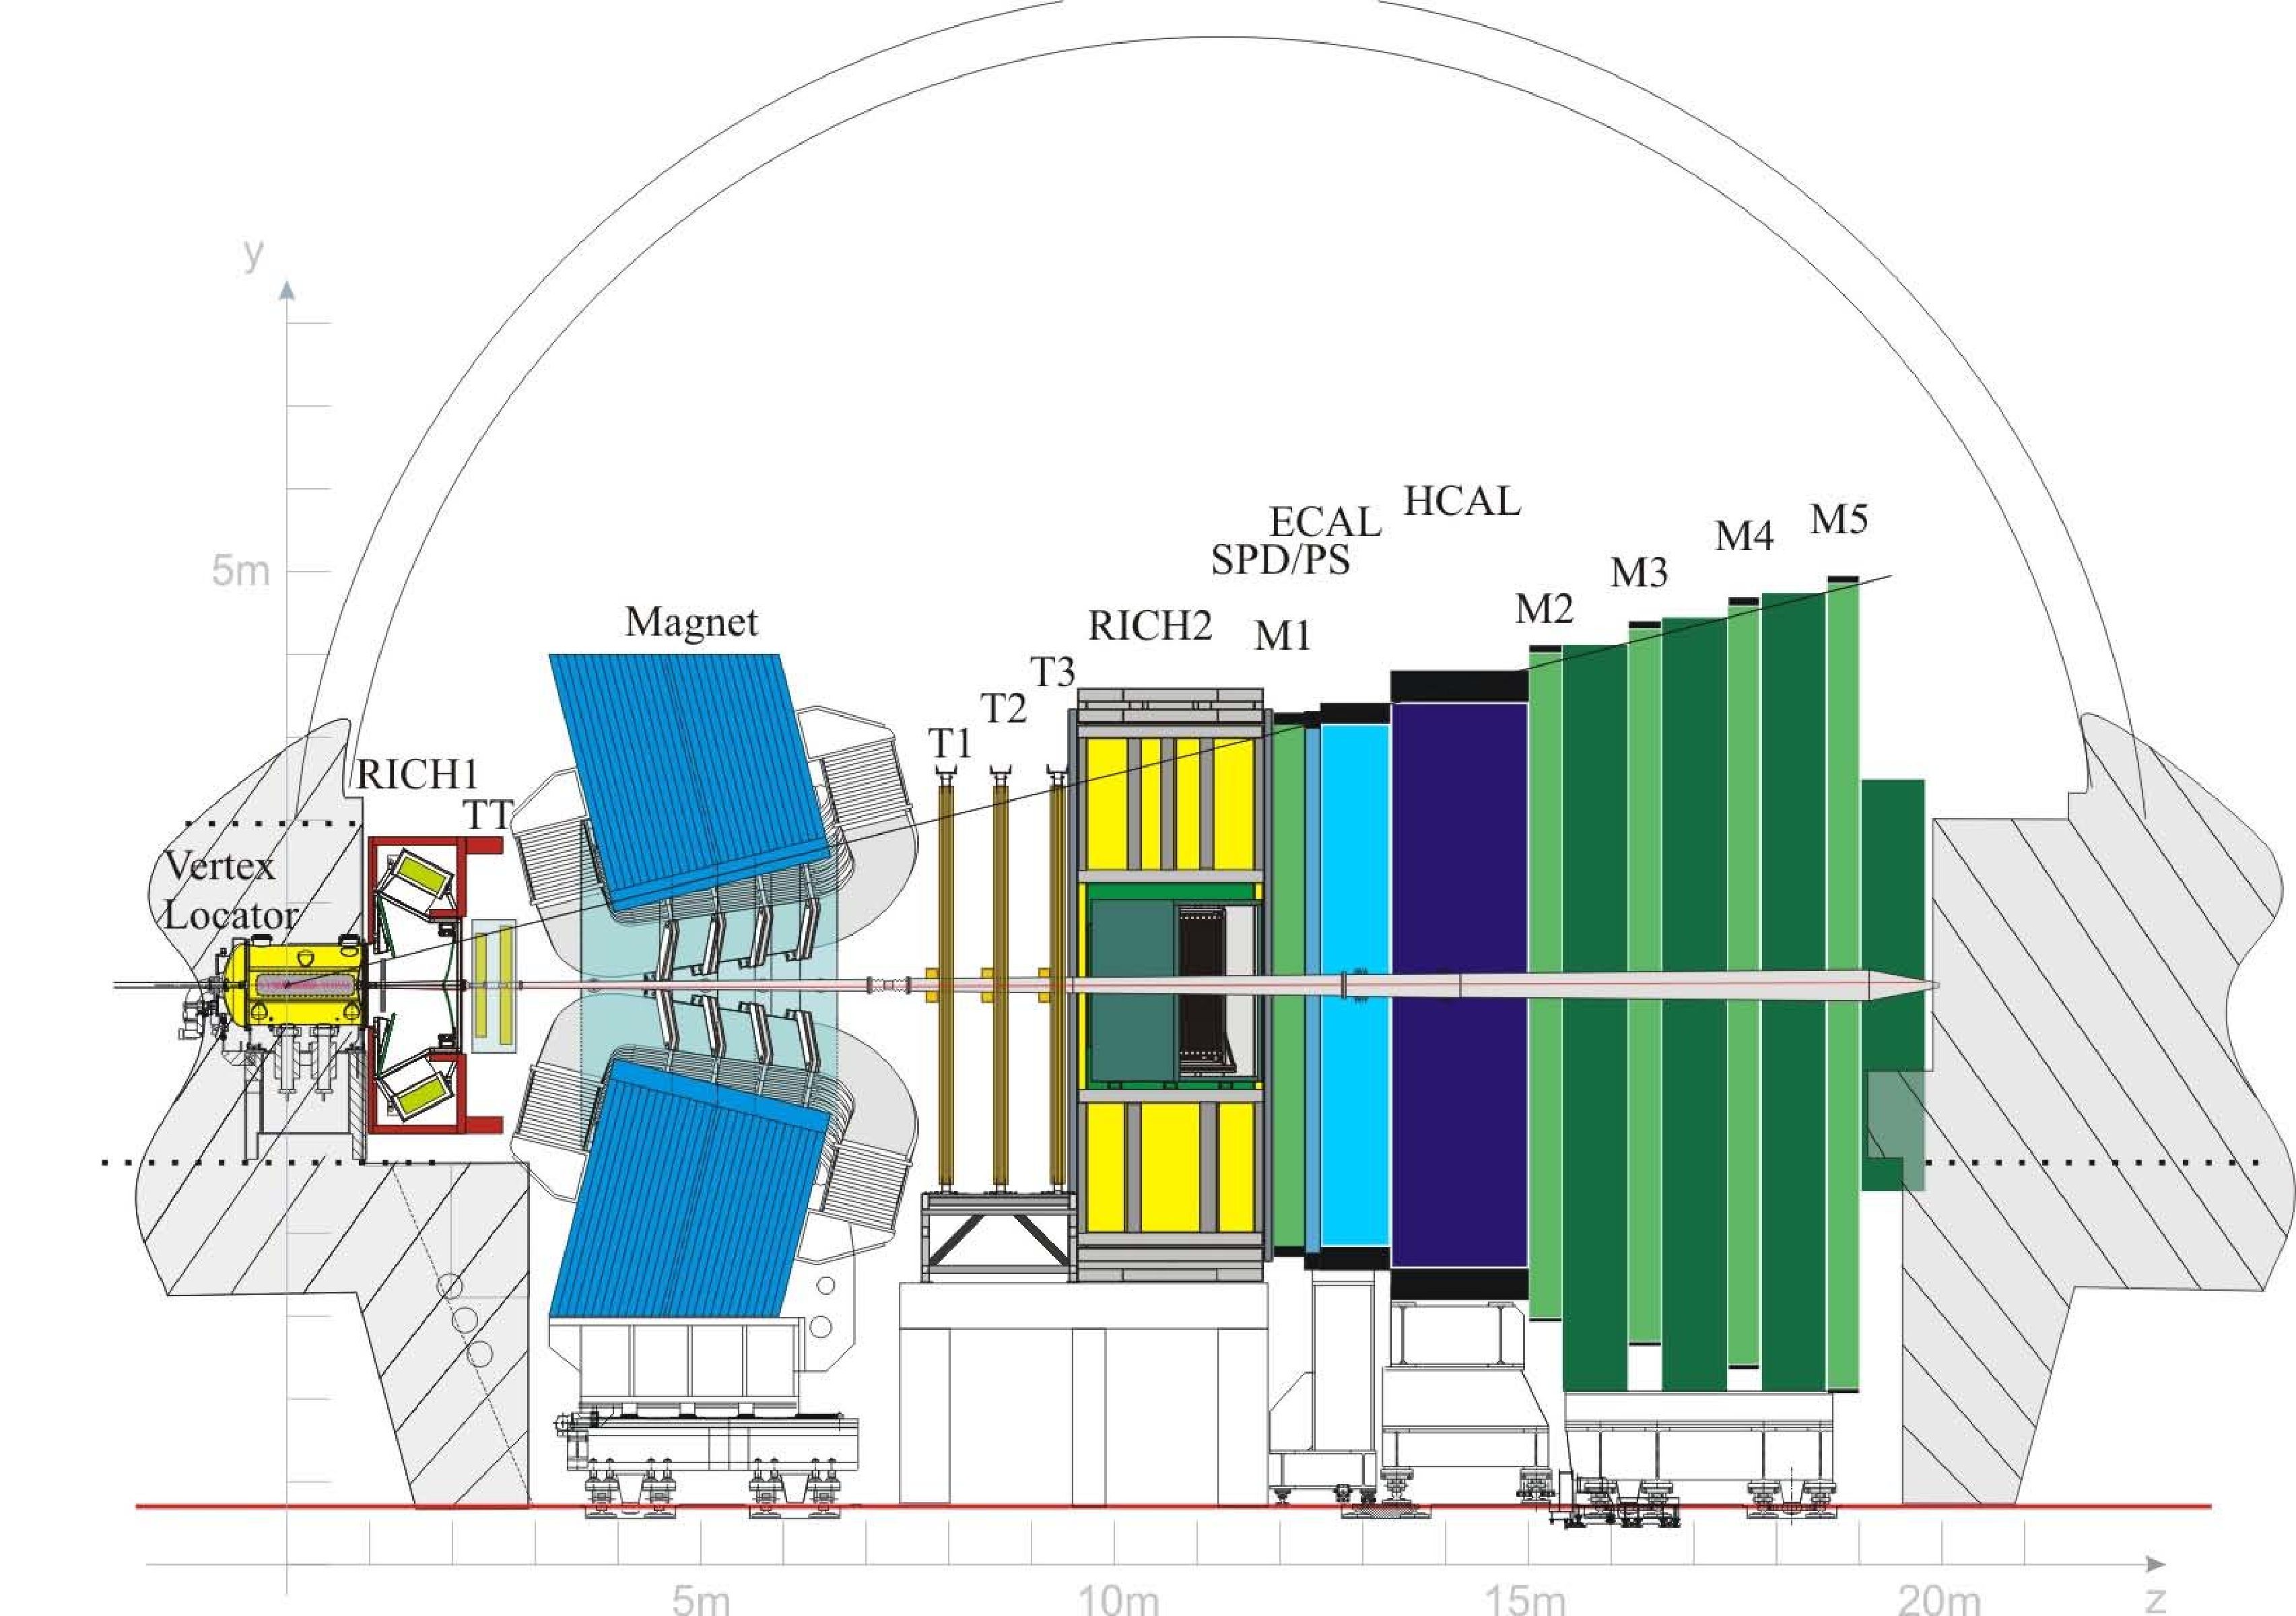
\includegraphics[scale = 0.25]{figs/detector/lhcbdet.pdf}
	\caption{Schematic slice of \Gls{LHCb} detector in the $y,z$ plane where $z$ is defined to be the direction parallel to beamline, and $x,y$ define the plane perpendicular to the beamline. $\theta$, the opening polar in the y-z plane with $\theta$ = 0 along the $z-axis$. Figure from \cite{LHCbdetector}.}
	\label{fig:LHCbDetector}
\end{figure}


\Gls{LHCb}, seen in~\autoref{fig:LHCbDetector}, differs from the other general purpose detectors on the \Gls{LHC} ring as its main aim is to study properties of heavy particles containing $b$ or $c$ quarks. This is possible as this \DIFdelbegin \DIFdel{experiments }\DIFdelend \DIFaddbegin \DIFadd{experiment }\DIFaddend was designed to have \DIFdelbegin \DIFdel{the }\DIFdelend \DIFaddbegin \DIFadd{a }\DIFaddend geometrical acceptance and unique vertex resolution\DIFaddbegin \DIFadd{, }\DIFaddend as well as excellent particle identification (\Gls{PID})\DIFaddbegin \DIFadd{, }\DIFaddend suitable for beautiful and charming physics.

Studies of $B$ mesons can happen either at positron-electron colliders or at hadron colliders. The advantage of positron-electron \DIFdelbegin \DIFdel{collider }\DIFdelend \DIFaddbegin \DIFadd{colliders }\DIFaddend is that the information about all the event is known, as just two $B$ mesons and nothing else is produced in \DIFaddbegin \DIFadd{the }\DIFaddend collisions. This gives an overall constraint on collision information, unlike in the hadron collider $B$ factory, \gls{LHCb}. Contrary to the two general purpose detectors at \gls{LHC}, where the collisions \DIFdelbegin \DIFdel{are occurring }\DIFdelend \DIFaddbegin \DIFadd{occur }\DIFaddend in the centre of the detector, \Gls{LHCb}'s collision point is located at one end of the detector, hence its description as a forward single-arm spectrometer. 

The disadvantage of not having an overall constraint on collision information is, however, compensated by the production mechanism of $b\bar{b}$ and $c\bar{c}$ in $pp$ interactions, which occurs predominantly via gluon-gluon fusion. In this process, each gluon will carry part of proton's momentum. If the two gluons from two protons carry significantly different \DIFdelbegin \DIFdel{momentum}\DIFdelend \DIFaddbegin \DIFadd{momenta}\DIFaddend , the $b\bar{b}$ system will be boosted with respect to the $pp$ rest frame, either in the forward or backward cone \DIFdelbegin \DIFdel{closely }\DIFdelend \DIFaddbegin \DIFadd{close }\DIFaddend to the beamline, as can be seen in~\autoref{fig:Acceptance}(b).


\begin{figure}
	\centering
	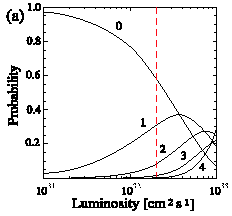
\includegraphics[width=0.45\linewidth]{figs/detector/license/croped.pdf}%
	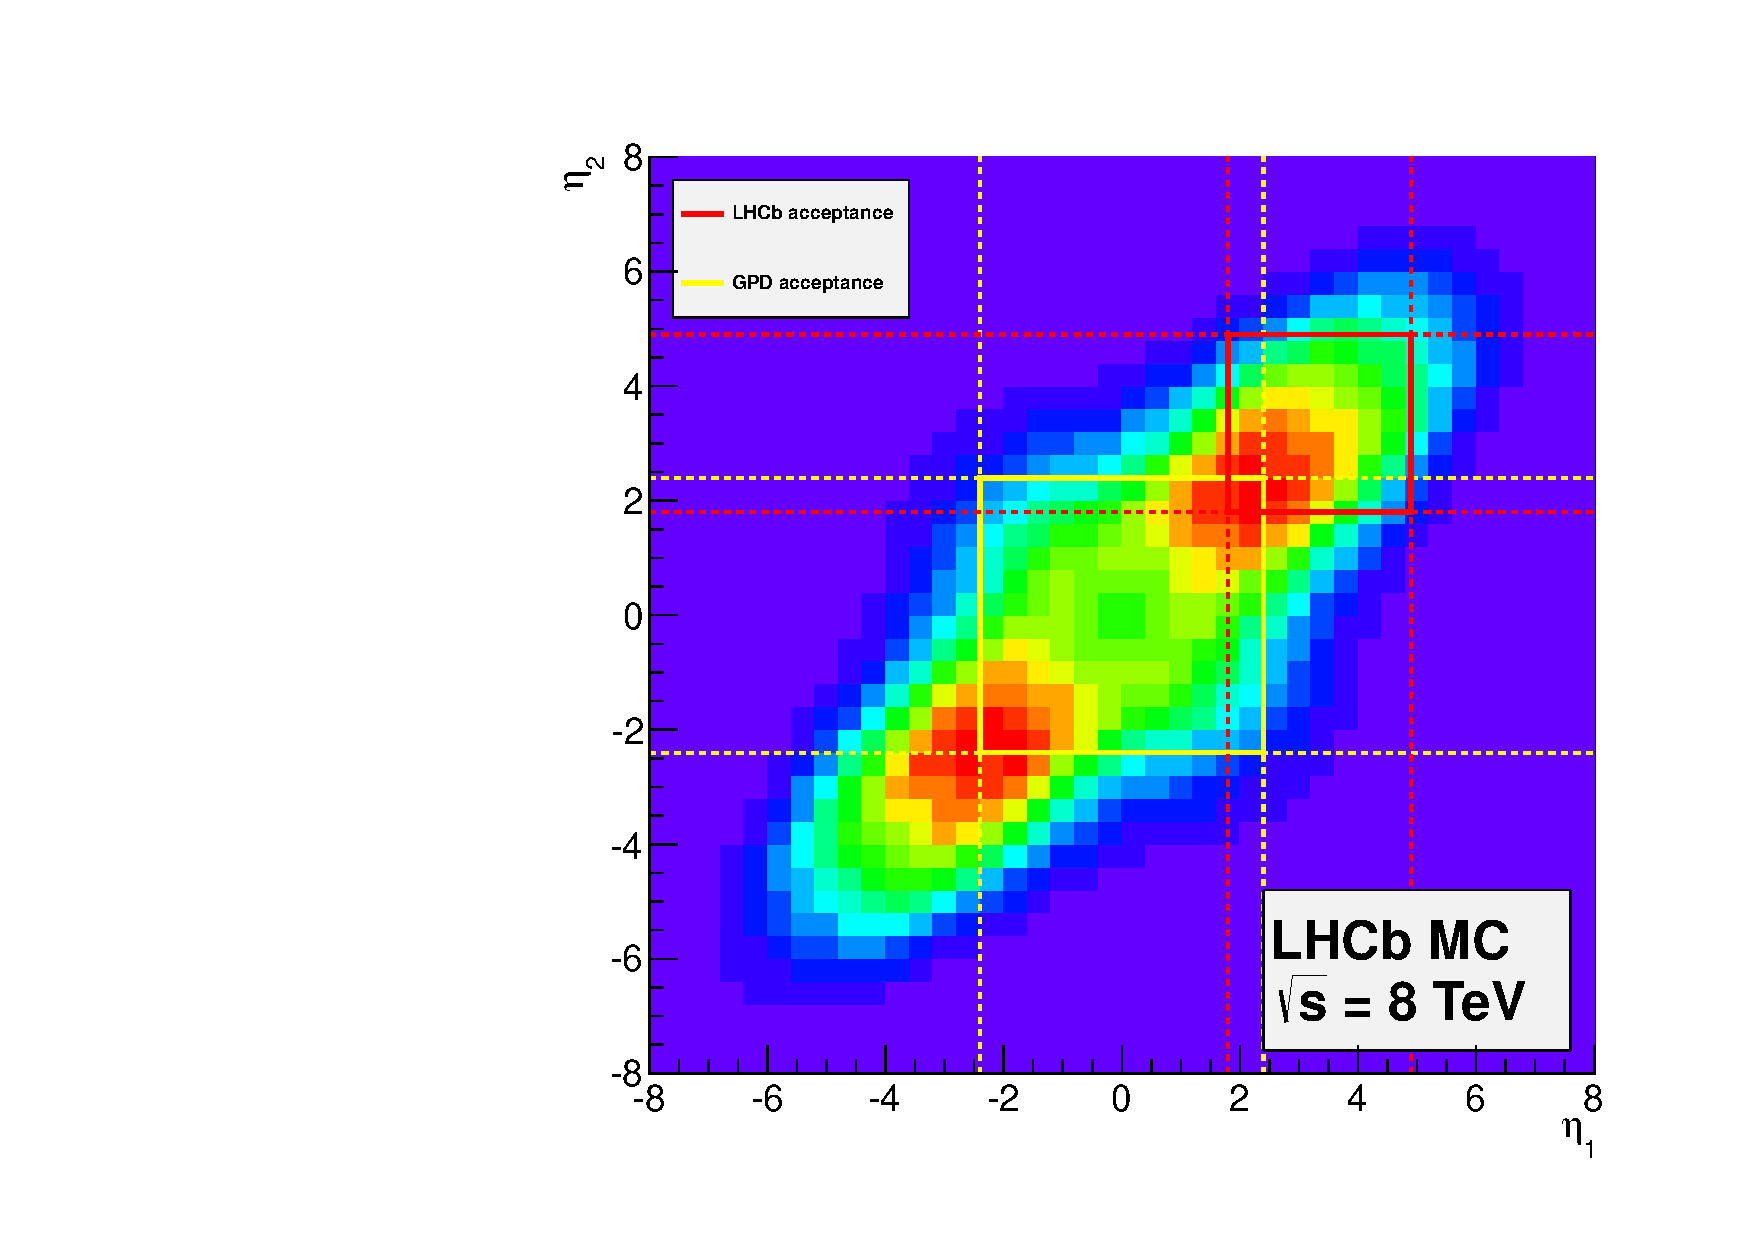
\includegraphics[width=0.5\linewidth]{figs/detector/Acceptance.pdf}\put(-10,170){(b)}
	\caption{(a) Probability of interaction per bunch crossing as a function of instantaneous luminosity. Figure from \cite{Raven:2007zi}. (b) Angular production and acceptance of the $b$ (x-axis) $\bar{b}$ (y-axis) pair produced from \DIFaddbeginFL \DIFaddFL{a }\DIFaddendFL $pp$ collision at the LHC. The acceptance of the LHCb detector is the red box and the acceptance of the General Purpose Detector is shown in the yellow box. \Gls{LHCb} covers the region with highest production cross-section at 8 \tev. These plots were produced using a Pythia 8.1 \cite{pythia8} simulation. Figure from \cite{acceptance}.}
	\label{fig:Acceptance}
\end{figure}

The angular coverage of \Gls{LHCb} is formally defined using pseudorapidity $\eta$, 

\begin{equation}
	\eta = -\ln \Big(\tan\frac{\theta}{2}\Big)
\end{equation}	
where $\theta$ is the polar angle measured from the beam axis. The \Gls{LHCb} detector was built to cover the region $2<\eta<5$. The production cross-section of the fundamental process of $pp\rightarrow b\bar{b}X$ was measured in this region yielding, $\sigma (pp\rightarrow b\bar{b}X)$= 75.3$\pm$5.4$\pm$13.0 $\mub$ at 7 \tev \cite{LHCb-PAPER-2010-002} and 144$\pm$1$\pm$21 $\mub$ at 13 \tev \cite{LHCb-PAPER-2016-031}, which shows that the production cross-sections scales roughly linearly with the centre-of-mass energy. Assuming \DIFaddbegin \DIFadd{the }\DIFaddend design conditions of \gls{LHCb}, listed in~\autoref{tab:runcond}, 2$\fb^{-1}$ of data (eqvivalent to \DIFaddbegin \DIFadd{the }\DIFaddend 2012 dataset) would correspond to $10^{12}$ \DIFdelbegin \DIFdel{of }\DIFdelend $b\bar{b}$ pairs being produced in a full 4$\pi$ region with 27\% of these $b\bar{b}$ pairs produced in the \gls{LHCb} acceptance. The summary of \gls{LHCb} running conditions is also provided in~\autoref{tab:runcond}. The analysis of \Bmumumu is done with \DIFaddbegin \DIFadd{the }\DIFaddend Run \Rn{1} and 2016 dataset. 

Despite the impressive statistics of $b\bar{b}$ pairs available to \Gls{LHCb}, the bottleneck in terms of data collection arises from the much more copious inelastic background. That mostly originates from soft \gls{QCD} processes which are related to the amount of pile-up, the visible number of $pp$ \DIFdelbegin \DIFdel{interaction }\DIFdelend \DIFaddbegin \DIFadd{interactions }\DIFaddend in the visible events. By looking at the probability of the number of $pp$ interaction per bunch crossing as a function of luminosity, shown in~\autoref{fig:Acceptance}(a), it can be noted that the maximum probability for only one $pp$ interaction (and hence minimizing the background) is found to be at $\sim 2 \times10^{32} \mathrm{cm^{-2} s^{-1}}$.  This was the reason behind \DIFaddbegin \DIFadd{the }\DIFaddend \gls{LHCb} design luminosity. Subsequently it has been found that it is more optimal to run at a higher luminosity of $\sim 4 \times10^{32} \mathrm{cm^{-2} s^{-1}}$ but then implement a set of global event cuts (GEC). Only events with 600 (in 7,8 \tev) and 450 (in 13 \tev) hits and less, corresponding to the track density in the particular part of the detector, are allowed to be processed.
As the majority of the branching fractions at \gls{LHCb} are measured with respect to other branching fractions, there is no bias \DIFdelbegin \DIFdel{being }\DIFdelend introduced by the GECs. 

As \Gls{LHCb} requires much lower luminosity compared to other \gls{LHC} detectors, there is an LHCb-specific control of luminosity known as \textit{luminosity levelling}, shown in~\autoref{fig:lhcbintlumi}. This procedure achieves stable instantaneous luminosity by controlling that the two beams do not collide straight head-on at collision point, but are moved with respect to each other. It limits the effects of luminosity decay, which can lead to trigger alterations during specific data taking run, resulting in systematic uncertainties.



%The summary of \gls{LHCb} running conditions is provided in~\autoref{tab:runcond}, showing the evolution of the instantaneous luminosity as well as the frequency of collisions compared to the design proposal.
%Formally \Gls{LHCb}   detector is placed along the beamline, where $x,y,z$ a spectrometer which cover the region of 300 \mrad defined a
%http://lhcb.web.cern.ch/lhcb/speakersbureau/excel/default.html

%\begin{figure}
%	\centering
%	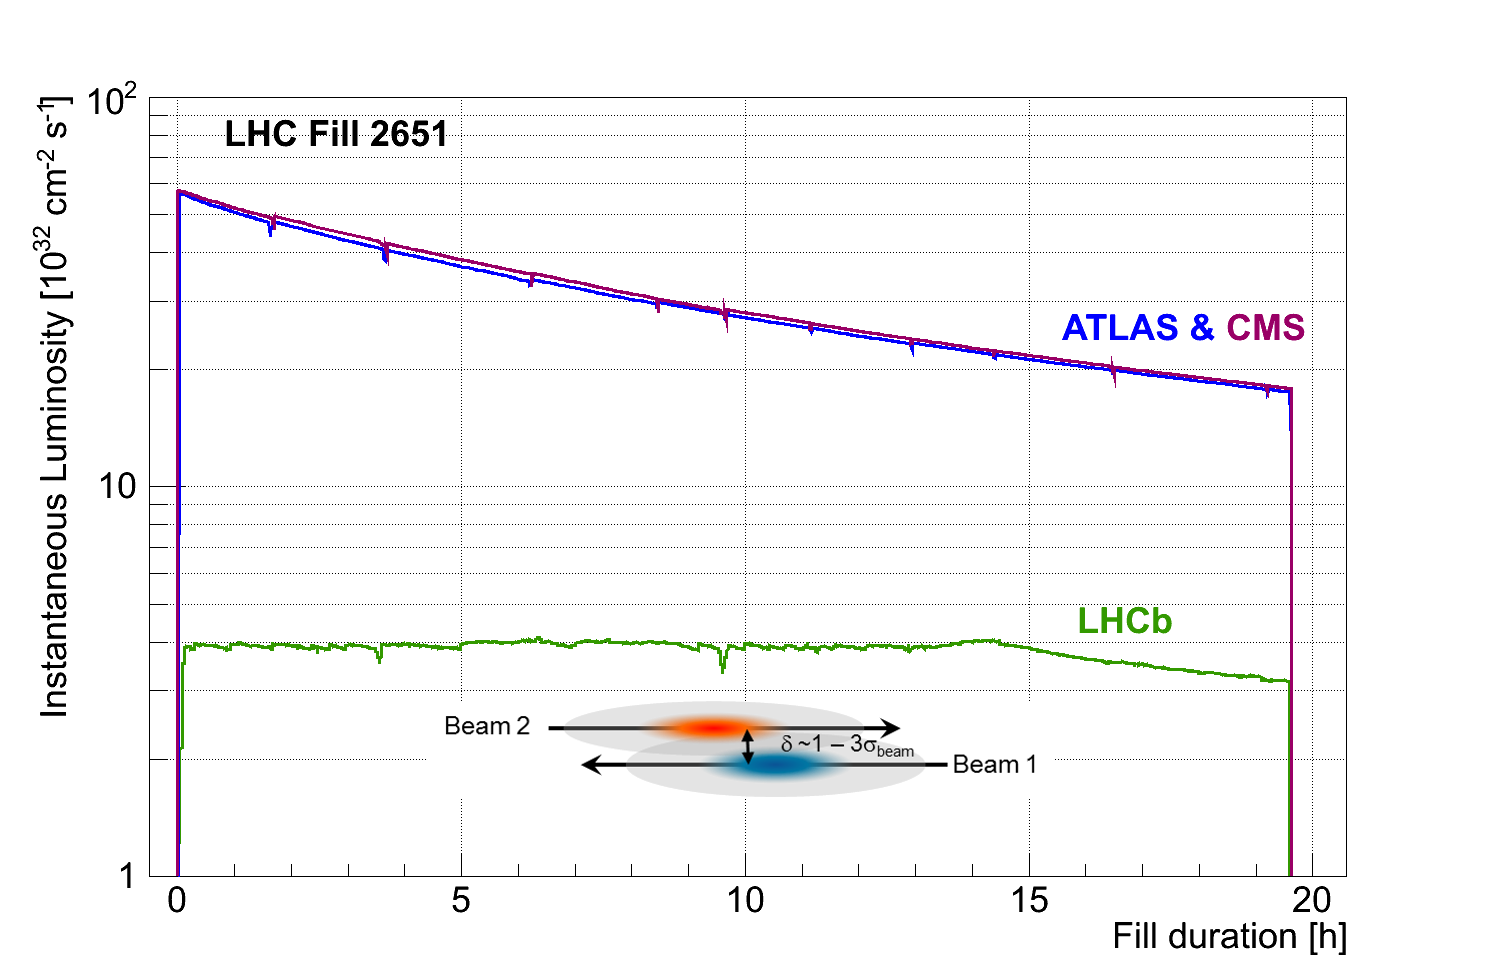
\includegraphics[scale = 0.5]{figs/detector/lumicompare.png}
%	\caption{Integrated luminosity collected in different years of data-taking. This plot is taken from \cite{lumiover}.}
%	\label{fig:lhcbintlumi}
%\end{figure}



\begin{table}[!h]
	\centering
%	\hspace*{-0.8cm}
	\begin{tabular}{l c c c }
		\toprule
		Year & $\sqrt{s}$ & $\mathcal{L}$  & Integrated Recorded Luminosity \\ 
		 & [\tev] & [$\times10^{32} \rm{cm^{-2}s^{-1}}$] & [$\rm{fb}^{-1}$] \\ \hline
		Design & Up to 14 & 2 & - \\
		2011  \rdelim\}{2}{1.5cm}[Run \Rn{1}] & 7 & $\sim$ 3.0-3.5 & 1.1 \\
		2012 & 8 & $\sim$ 4.0 & 2.1 \\
		2015 \rdelim\}{3}{1.5cm}[Run \Rn{2}] & 13 & $\sim$ 0.5-4.5 & 0.3 \\      
		2016 & 13 & $\sim$ 4.0 & 1.7  \\      
		2017 & 13 & $\sim$4.0-6.0 & 1.7 \\\bottomrule      
	\end{tabular}
	\caption{Running conditions of \gls{LHC} and \Gls{LHCb} in different years of data-taking. The statistics of \gls{LHCb}'s instantaneous luminosity, $\mathcal{L}$ is extracted using run database information. Run \Rn{2} data-taking finishes in 2018.}
	\label{tab:runcond}
\end{table}   

\begin{figure}
	\centering
%	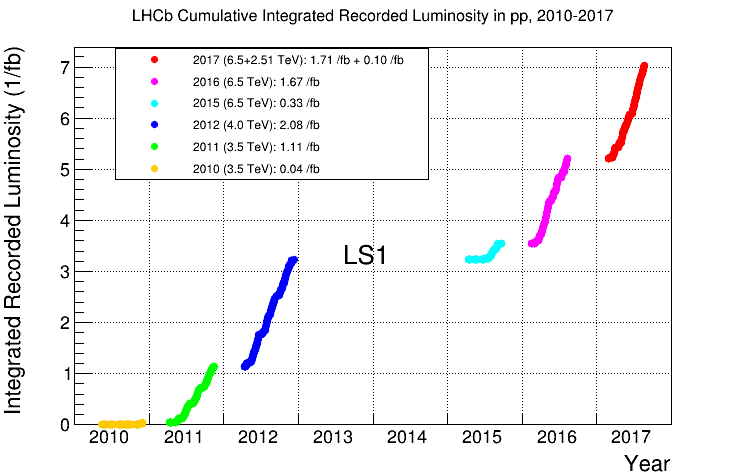
\includegraphics[width = 0.5\textwidth]{figs/detector/intlumi.png}\put(-15,100){(a)}
        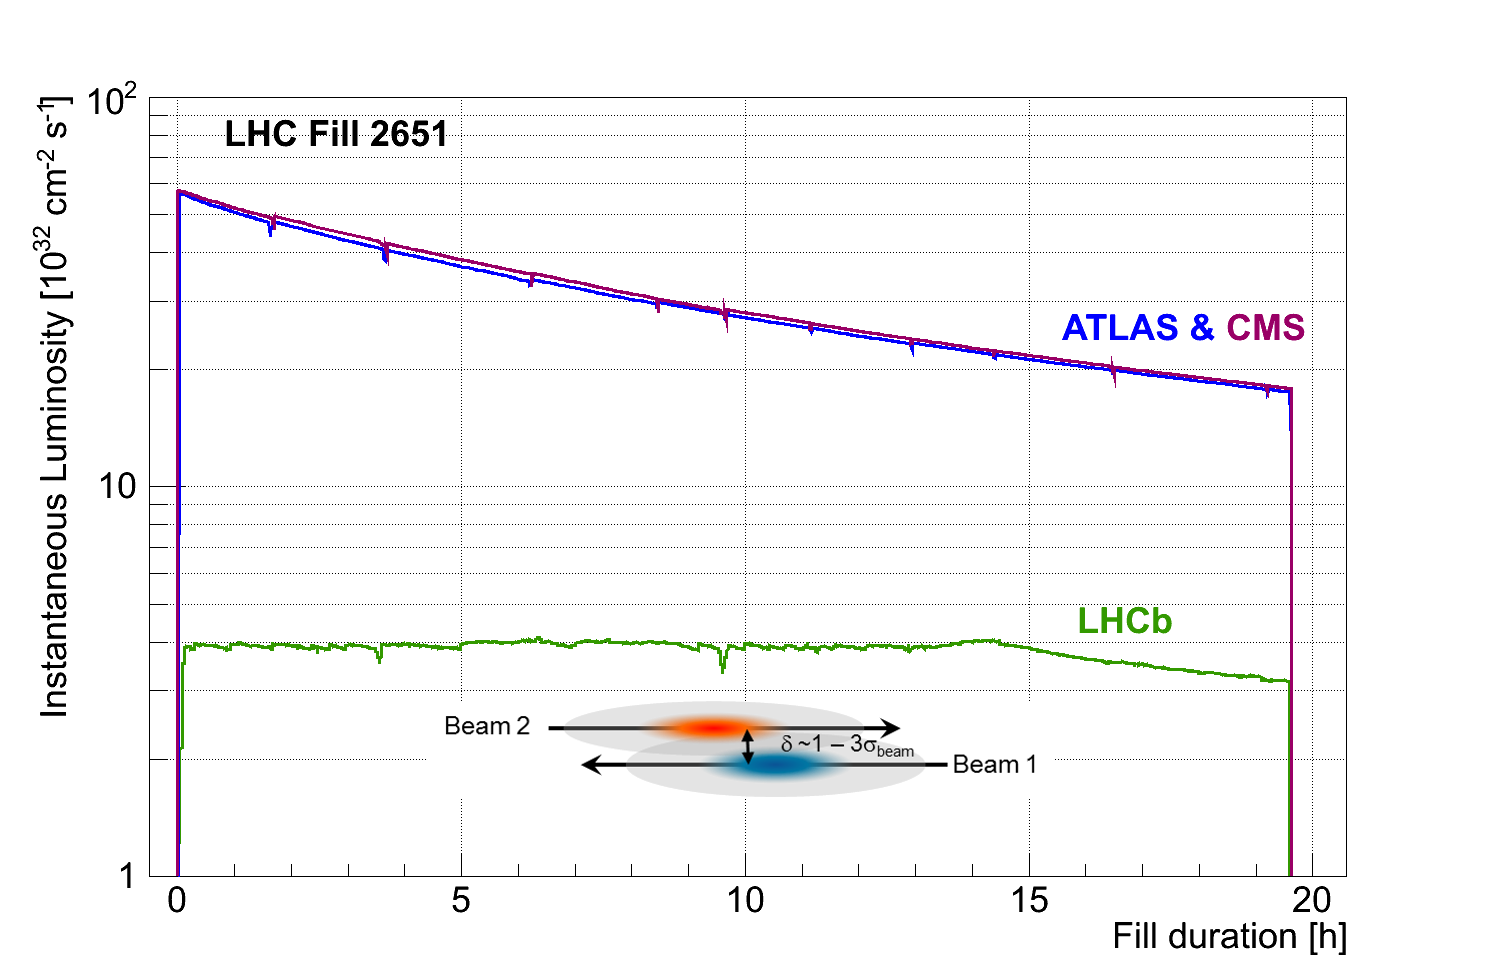
\includegraphics[width = 0.65\textwidth]{figs/detector/lumicompare.png}%\put(-15,100){(b)}
	%\caption{(a) Integrated luminosity collected in different years of data-taking. This plot is taken from \cite{lumiover}. (b)
	\caption{Development of the instantaneous luminosity for \Gls{ATLAS}, \Gls{CMS} and \Gls{LHCb} during \DIFaddbeginFL \DIFaddFL{a random representative }\DIFaddendFL LHC fill\DIFdelbeginFL \DIFdelFL{2651. }\DIFdelendFL \DIFaddbeginFL \DIFaddFL{. }\DIFaddendFL After ramping to the desired value of $4\times10^{32}\mathrm{cm^{-2}s^{-1}}$
	for \Gls{LHCb}, the luminosity is kept stable in a range of 5$\%$ for about 15 hours by adjusting the transversal beam overlap. The difference in luminosity towards the end of the fill between \Gls{ATLAS}, \Gls{CMS} and \Gls{LHCb} is due to the difference in the final focusing at the collision points, commonly referred to as the beta function, $\beta^{*}$. This plot was obtained from \cite{LHCb-DP-2014-002}.}
	\label{fig:lhcbintlumi}
\end{figure}

In the following sections, a brief discussion of the different subdetectors, shown in~\autoref{fig:LHCbDetector}, is presented. The vertexing at \gls{LHCb} is performed with the vertex locator system, also known as the VELO, \DIFaddbegin \DIFadd{and }\DIFaddend is described in~\autoref{velosys}. The tracking system at \gls{LHCb} consisting of trackers before \DIFaddbegin \DIFadd{the }\DIFaddend magnet (TT), and three tracking stations behind the magnet (T1, T2, T3) is highlighted in~\autoref{tracksys}. The particle identification is provided by two Ring Imaging \v{C}erenkov counters (RICH1 and RICH2), which are detailed in~\autoref{richsec}. No particle physics experiment is complete without a calorimeter system, discussed in~\autoref{calosys}, which consists of a Scintillator Pad Detector (SPD), Preshower (PS), an electromagnetic calorimeter (ECAL) and finally a hadronic calorimeter (HCAL). The muon system positioned at the end of the detector, consisting of five muon chambers is described in~\autoref{muonsys}. The trigger chain as well as the simulation chain are discussed in~\autoref{triggerchap} and~\autoref{simulationchap}. Particular emphasis is given to the muon detectors and the simulation of \gls{LHCb}.

%\color{red}{ \mybox{Sally} corrected until now} \color{black}.

\section{VErtex LOcator }
\label{velosys}
The subdetector closest to the collision point is the VErtex LOcator (\Gls{VELO}). This silicon-strip based detector, that extends 1 \m along the beam axis, is primarily used to distinguish signal-like events from prompt background. The typical \DIFdelbegin \DIFdel{differing }\DIFdelend property of a $b$-hadron decay \DIFdelbegin \DIFdel{includes }\DIFdelend \DIFaddbegin \DIFadd{include }\DIFaddend large impact parameter (\Gls{IP}), the minimal distance between the track and a primary vertex, in addition to significantly higher transverse momentum, $p_{T}$. Therefore, the main tasks of this subdetector \DIFdelbegin \DIFdel{is }\DIFdelend \DIFaddbegin \DIFadd{are }\DIFaddend to find: 
 \begin{itemize} 
\item primary vertices
\DIFdelbegin \DIFdel{positions
}\DIFdelend \item secondary vertices of short-lived particles (heavy quark hadrons)
\item tracks that did NOT originate from \DIFaddbegin \DIFadd{the }\DIFaddend primary vertex
 \end{itemize} .


\begin{figure}[!h]
	\centering
	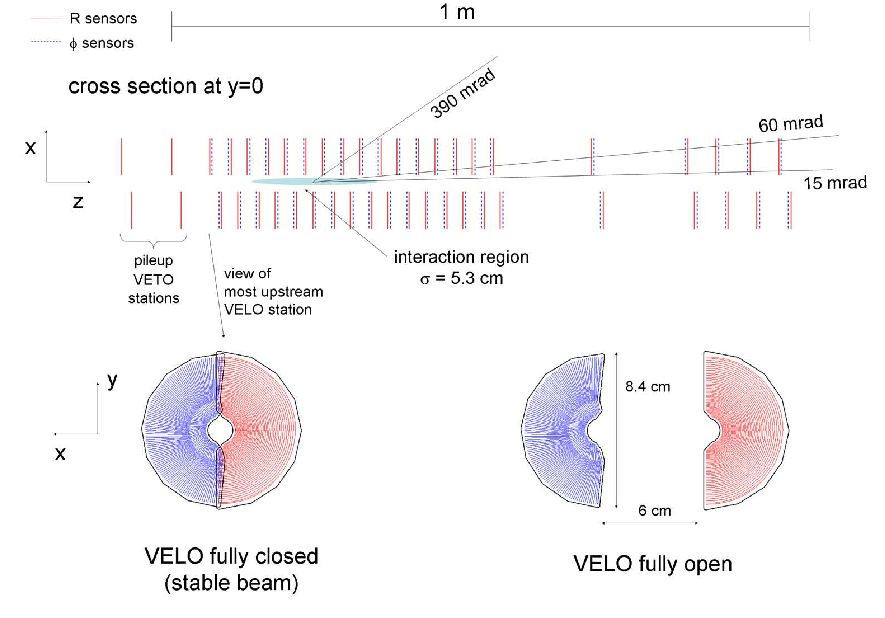
\includegraphics[width = 0.75\textwidth]{figs/detector/license/Velo_croped.pdf}
        %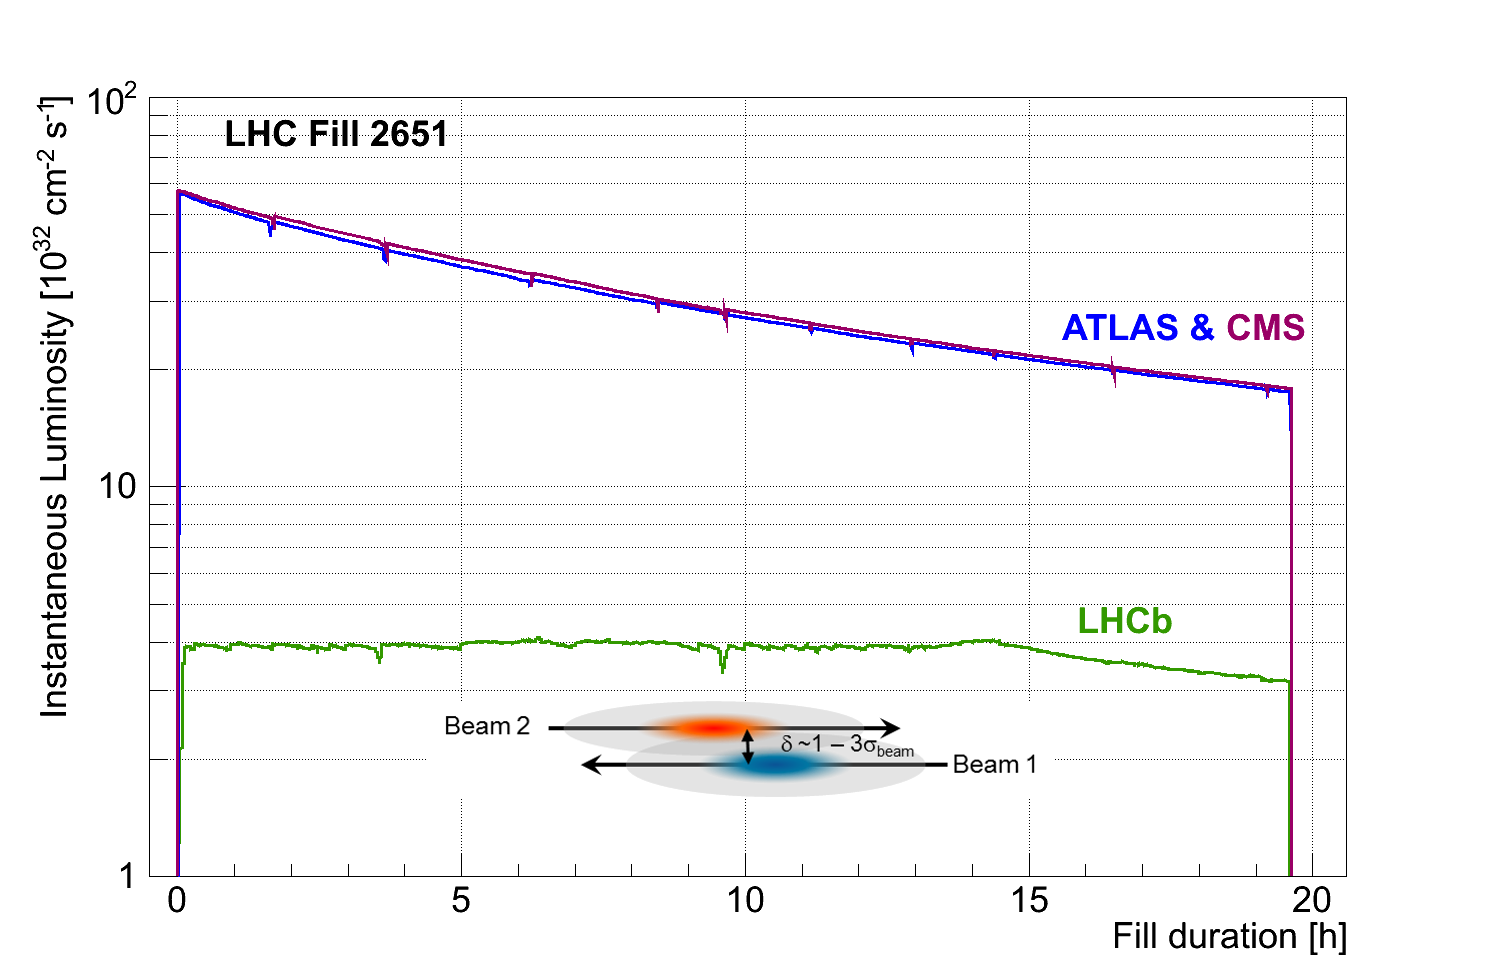
\includegraphics[width = 0.5\textwidth]{figs/detector/lumicompare.png}
	\caption{Schematic plot of the \Gls{VELO} detector configuration along the beam pipe showing the layout as well as positions while in stable beams (discs have slight overlap) and injection. Figure from \cite{det_paper}.}
	\label{fig:veloover}
\end{figure}

The detector consists of two sets of 21 silicon modules positioned around the beam pipe, where each module has 2 types of half-moon-shaped discs as seen in~\autoref{fig:veloover}. In the first type, the strips are arranged to provide radial information ($R$), whereas the second type provides azimuthal ($\phi$) information. As $pp$ collisions bring a high dose of radiation to this detector, the first sensitive strip starts at a distance of 8 \mm once stable beams are declared. Throughout the beam injection, when the beam radius may be larger, the two sets are moved 3 \cm away, perpendicular to the beam axis. For the $R$ sensor, the individual module's strip pitch, the distance between two strips, varies from 38 $\mum$ to 102 $\mum$ away from the beam pipe, so that the hit occupancy is roughly even as a function of distance away from the beam pipe. Each \Gls{VELO} half is kept within an aluminium welded box causing material overlap once stable beams are declared. These boxes form their own vacuum which is separated from the nominal \gls{LHC} vacuum in order to protect the detector from any electromagnetic interference with the beam. 

This setup brings outstanding hit resolution (4-40$\mum$), which in turn allows for very high \gls{IP} and very good primary vertex (\gls{PV}) resolution, as seen in~\autoref{fig:veloIPres}(a)(b). This is indispensable not only in order to perform the precise measurements of $B$ and $D$ lifetimes, but also to resolve oscillations caused by $B^{0}_{s}-\bar{B}^{0}_{s}$ mixing occurring at a 3 trillion \hz rate. As will be seen later, this excellent resolution is also very important for the detection of decays with neutrinos in the final state.

\begin{figure}[!h]
	\centering
	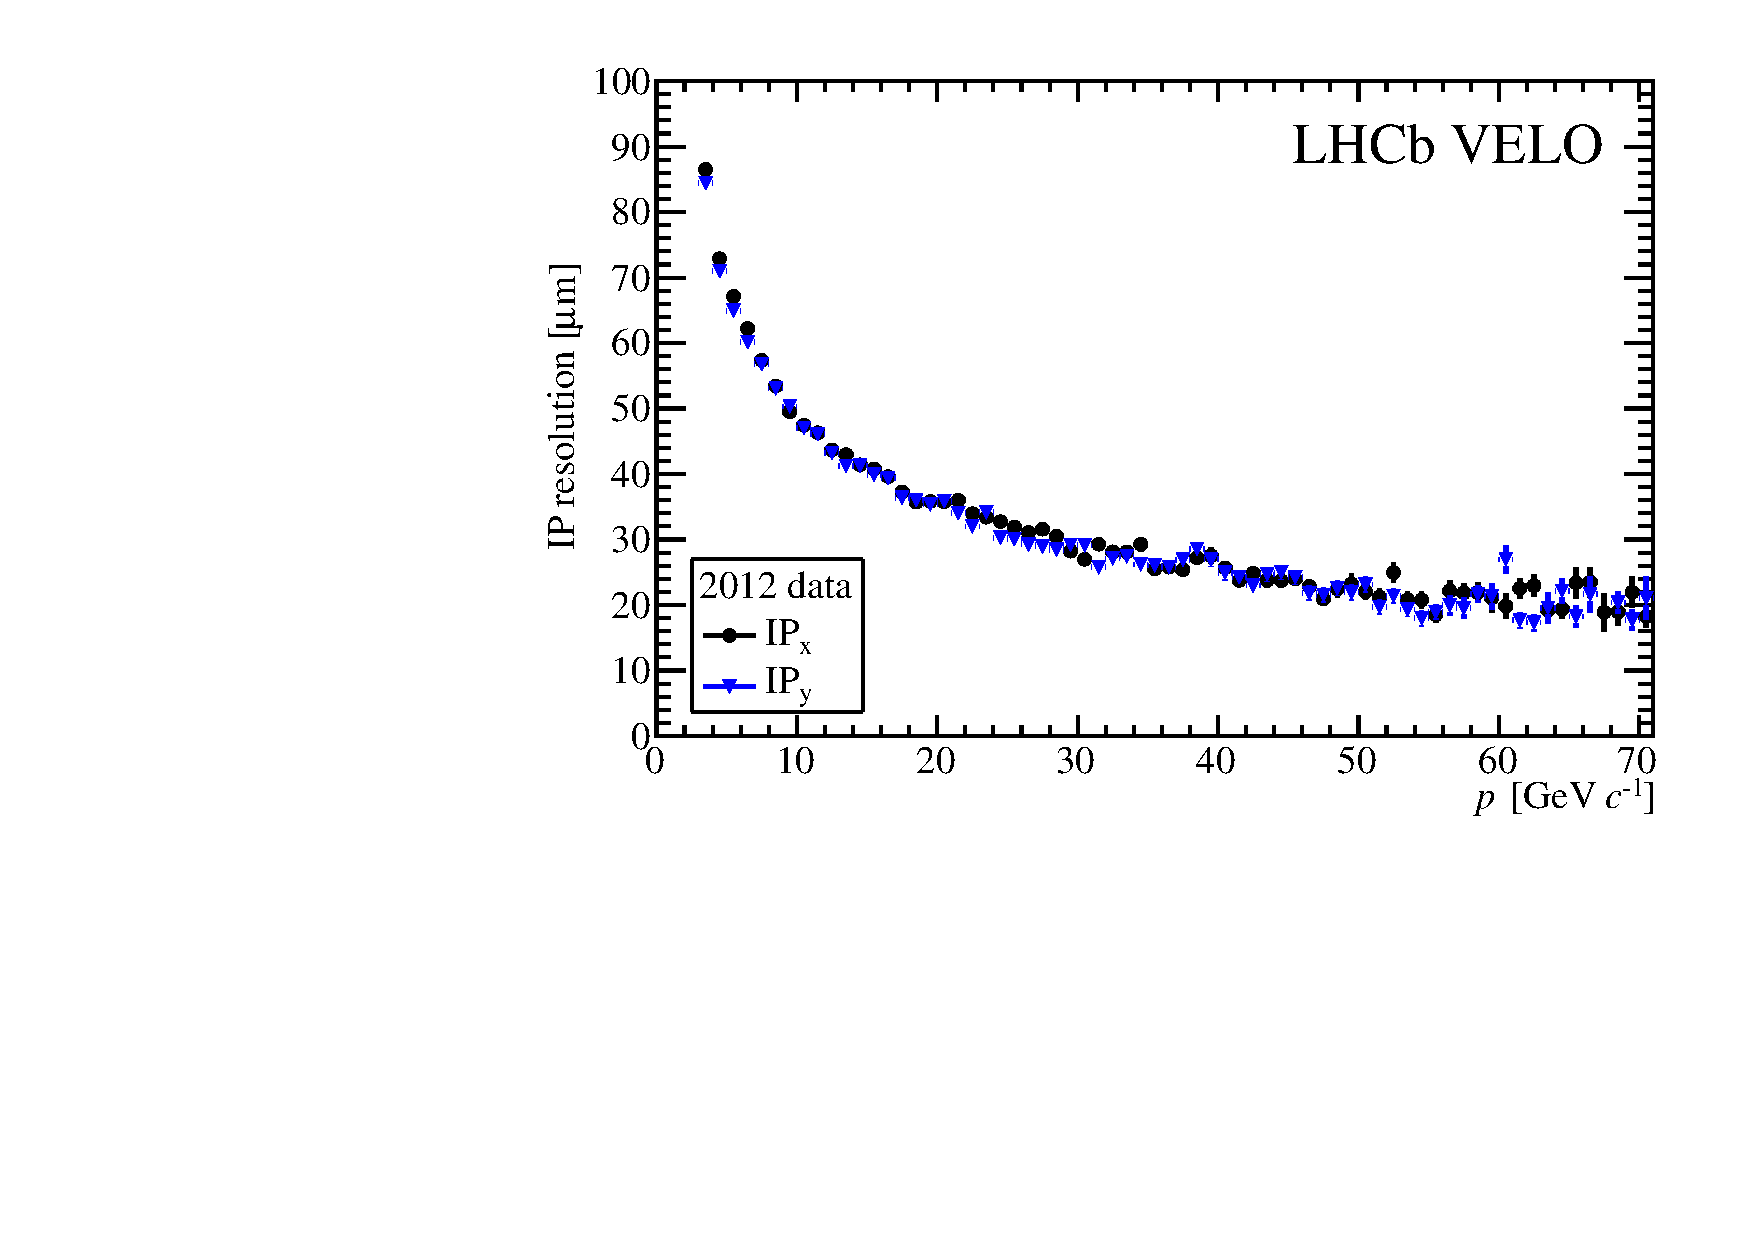
\includegraphics[width = 0.5\textwidth]{figs/detector/IPRes-Vs-P-CompareIPxIPy-2012.pdf}\put(-50,70){(a)}
        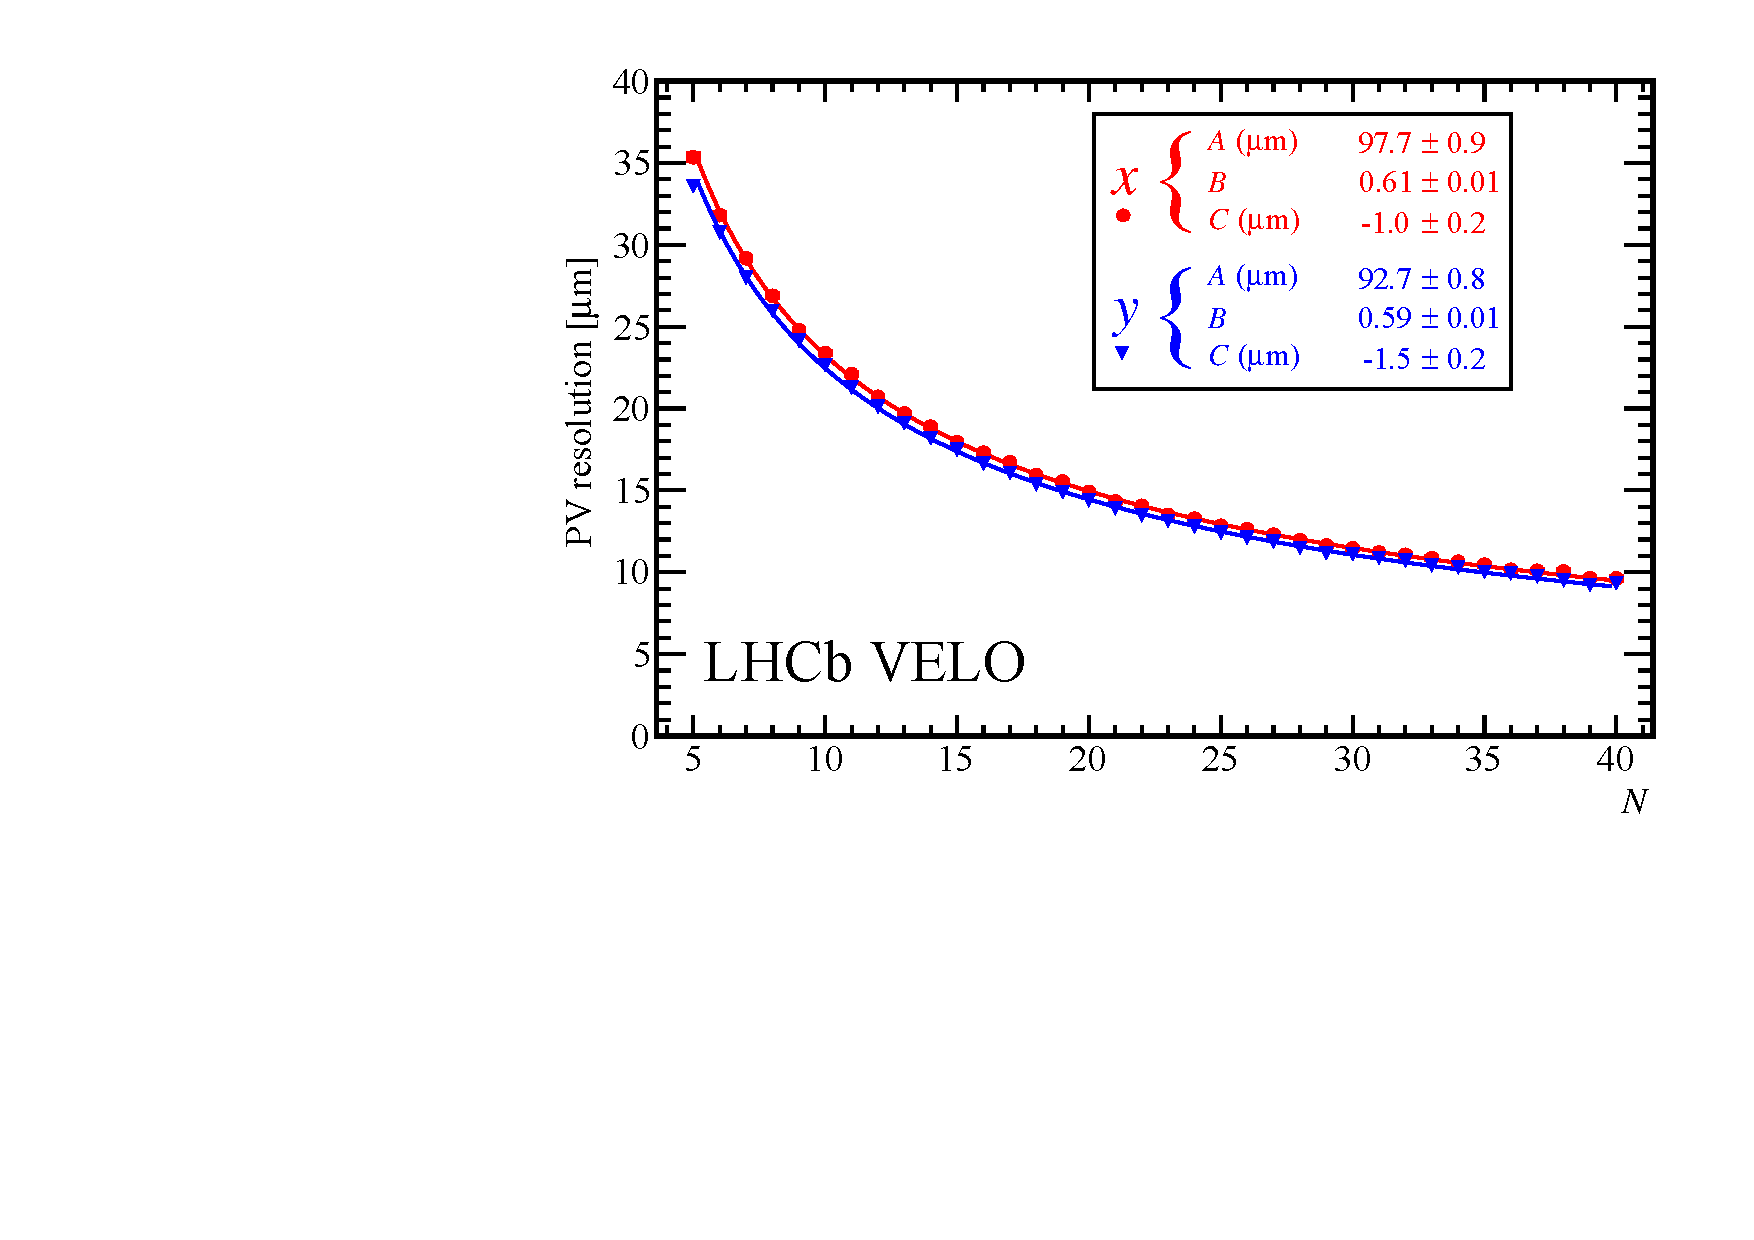
\includegraphics[width = 0.5\textwidth]{figs/detector/ResXY_1PV_2011Data.pdf}\put(-50,70){(b)}
	\caption{Two key variables which quantify performance of the \Gls{VELO} detector. (a) \Gls{IP} resolution which is worse for low momentum tracks and (b) \Gls{PV} resolution dependent on the number of tracks forming the primary vertex $N$. Figures from \cite{LHCbVELOGroup:2014uea}.}
	\label{fig:veloIPres}
\end{figure}


\section{Tracking System }
\label{tracksys}
In addition to tracking information provided by the \Gls{VELO}, the trajectories of charged particles are measured by a series of tracking subdetectors. The main task of these tracking subdetectors is to provide efficient reconstruction and precise measurement of a particle's momentum. There are four tracking stations apart from \Gls{VELO}: Tracker Turicensis (\Gls{TT}), positioned upstream from the magnet, and the \Gls{Tstation} tracking stations on the other side of the magnet. The dipole magnet with $\approx$ 4 Tm integrated field provides strength to bend charged particles in \DIFaddbegin \DIFadd{the }\DIFaddend horizontal plane.
% 10 m of charged trakcs
%with $p$ of 200 $\gev/c^{2}$.      

 Two different detection technologies are used in these trackers reflecting the nature of track occupancy as a function of polar angle. The \DIFdelbegin \DIFdel{tracker's part }\DIFdelend \DIFaddbegin \DIFadd{parts }\DIFaddend at small polar angles, \Gls{TT} station together with central region of \Gls{Tstation}, also known as \DIFaddbegin \DIFadd{the }\DIFaddend Inner Tracker (\Gls{IT}), \DIFdelbegin \DIFdel{expects }\DIFdelend \DIFaddbegin \DIFadd{expect }\DIFaddend higher occupancy and \DIFdelbegin \DIFdel{makes }\DIFdelend \DIFaddbegin \DIFadd{make }\DIFaddend use of the silicon microstrip detection mechanism. The outer part of \Gls{Tstation} stations, also known as the Outer Tracker (\Gls{OT}), is made of straw-tube detectors. Straw tubes measure the trajectory of the track by measuring the drift-time of ionized electrons. Use of the two technologies is illustrated in~\autoref{fig:tracktype}(a). 

\subsection{Tracking Algorithms} 
Different types of particles will leave different footprints in the detector. Charged particles will form tracks. Depending on the presence of hits in individual subdetectors, they are grouped into several categories, visualized in~\autoref{fig:tracktype}(b).

\begin{figure}[!h]
	\centering
	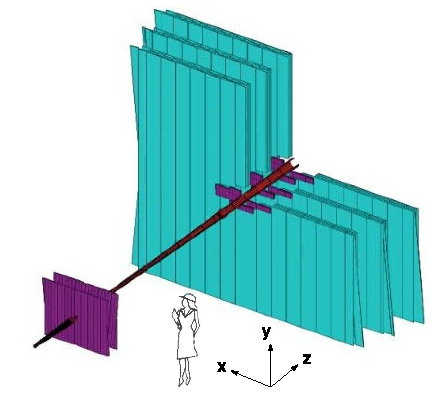
\includegraphics[width = 0.35\textwidth]{figs/detector/license/OT_crop.pdf}\put(-30,90){(a)}%
	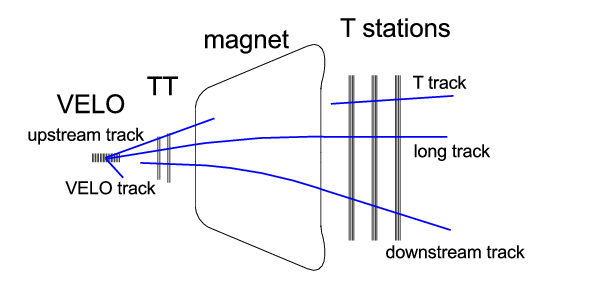
\includegraphics[width = 0.6\textwidth]{figs/detector/tracktype.png}\put(-30,90){(b)}
	\caption{ (a) Visualisation of use of different technology with silicon technology in violet and straw-tube technology in cyan. Figure from \cite{det_paper}. (b) Track types categorisation depending on which track stations provided hits. For the study of \Bmumumu decays, only \gls{longtrack}s are considered as muons will travel to the end of the detector leaving \DIFdelbeginFL \DIFdelFL{the }\DIFdelendFL hits all along. Figure from \cite{LHCb-DP-2013-002}.}
	\label{fig:tracktype}
\end{figure}

%http://iopscience.iop.org/article/10.1088/1748-0221/3/08/S08005/pdf
%https://twiki.cern.ch/twiki/bin/view/LHCb/TrackingEffAbsLength /secondary interactions - hadronic int.

Most of the physics analyses at \gls{LHCb}, as it is the case for the search of \Bmumumu, use only \gls{longtrack}s, tracks leaving hits in the \Gls{VELO} and \Gls{Tstation}, as they give most precise momenta measurements. There are also other types of tracks as indicated in~\autoref{fig:tracktype} but they are rarely used.
%VELO tracks leave hits only in $R$ and $\Phi$ sensor, but not in any other tracking stations. VELO tracks are formed by particles which must have left \Gls{LHCb} acceptance or they come from particles produced backwards and hence are useful for \gls{PV} reconstruction. Upstream tracks are formed by tracks leaving hits in \Gls{VELO} and \gls{TT} only. These are usually low momentum particles, which are bent out \Gls{LHCb} acceptance while traversing the magnet. Long-lived particles such as $\Lambda$ or $K^{0}_{s}$ will only decay outside of the \Gls{VELO} acceptance and hence will produce no hits until \Gls{TT} and \Gls{Tstation} forming downstream tracks. T-track is track type that only have hits in \Gls{Tstation}. Again this could be due to presence of long-lived particles or due to secondary interactions in the detector.   

In general, the track reconstruction software starts with \textit{pattern recognition}, where several hits in one part of a tracking subdetector are identified and form \textit{track seeds}, which are then extrapolated and combined with hits in other tracking subdetectors. The long track candidates are formed and fitted with a Kalman filter\cite{Hierk:684697}, where, because of the material present in the detector, corrections for energy losses as well as multiple scattering are incorporated.

In \gls{LHCb} there are types of tracks which are not really the trajectories of charged particles.
Sometimes the \textit{pattern recognition} may combine random hits into a track, which is then known as a \textit{ghost track}. On the other hand, it could also happen that several tracks are sharing the same hits, known as \textit{clone tracks}. The presence of these types of tracks are suppressed through the use of a neural network based variable (\Gls{pgh2}), which relies on \DIFaddbegin \DIFadd{the }\DIFaddend $\chi^{2}$ of the track fit, and information about missing hits along the trajectory to calculate its value.
%Presence of these tracks are heavily suppressed with different techniques - such as establishing ghost probability (\Gls{pgh2})- variable based on the output of neural network combining track $\chi^{2}$, quality of the track, and missing hits in the subdetectors.

When searching for a $b$-hadron decay, the mass of a candidate can be calculated from the 4-momenta of the decay products. Uncertainty on this mass is one of the crucial parameters to minimize as it enables a better separation between the identified signal and background. It strongly correlates with \DIFaddbegin \DIFadd{the }\DIFaddend momentum resolution that is obtained using \DIFaddbegin \DIFadd{the }\DIFaddend tracking system. \DIFdelbegin \DIFdel{Resulting }\DIFdelend \DIFaddbegin \DIFadd{The resulting }\DIFaddend relative momentum uncertainty (0.5-1.1\%) on \gls{longtrack}s using $J/\psi \rightarrow \mu^{+} \mu^{-}$ data can be seen in~\autoref{fig:momres}. It varies logarithmically with increasing momentum.


\begin{figure}[!h]
	\centering
	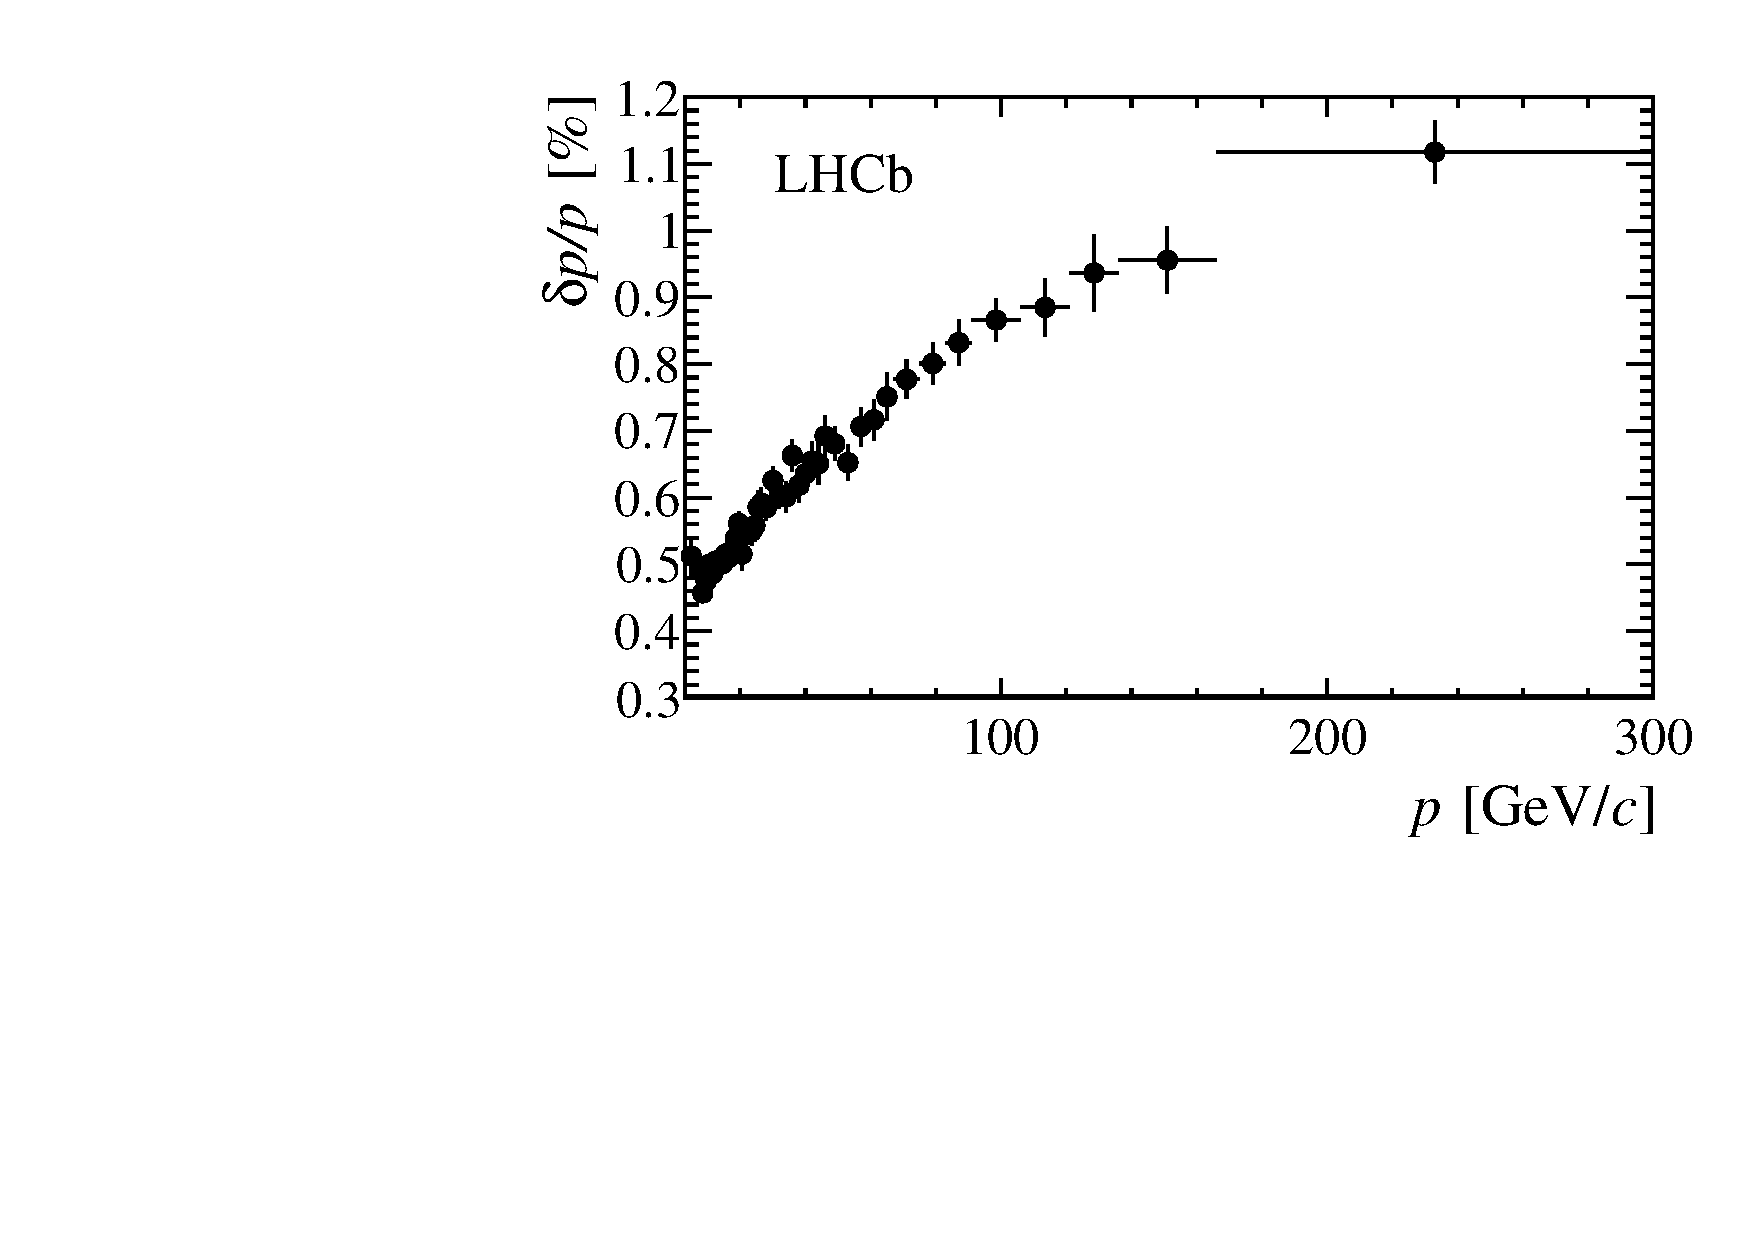
\includegraphics[width = 0.6\textwidth]{figs/detector/Fig17.pdf}
	\caption{Momentum resolution of \gls{longtrack}s measured at \gls{LHCb}. The decay channel $J/\psi \rightarrow \mu^{+} \mu^{-}$ is analysed for this purpose. Figure from \cite{LHCb-DP-2014-002}.}
	\label{fig:momres}
\end{figure}

\section{Ring Imaging \v{C}erenkov Detectors}
\label{richsec}
Particle identification, \Gls{PID}, at \Gls{LHCb} relies heavily on two dedicated Ring Imaging \v{C}erenkov subdetectors, \gls{RICH}. These detectors take advantage of the emission of \v{C}erenkov light, which happens when a charged particle travels through a medium at a speed faster than the phase velocity of light in that medium. This cone of light is emitted at an angle $\theta$ with respect to the charged particle's trajectory. Using the knowledge of \DIFaddbegin \DIFadd{the }\DIFaddend refractive index of the medium, $n$, and momentum $p$ that is measured using the tracking system, the mass $m$ of the particle can be obtained through:

\begin{equation}
	\cos\theta_{c} =  \frac{\sqrt{m^{2} + p^{2}}}{pn}.
\end{equation}

As the momentum is not an intrinsic property of a passing particle, the momentum identification range is limited by the choice of medium, also known as radiator. For very low-momentum particle, as $\cos\theta_{c} \rightarrow 1$ ($p=\sqrt{\frac{m^{2}}{n^{2}-1}}$), the particle is not producing any \v{C}erenkov light cone. At \DIFdelbegin \DIFdel{the }\DIFdelend very high momentum, as $\cos\theta_{c} \rightarrow 1/n$, there is \DIFaddbegin \DIFadd{a }\DIFaddend saturation point as all species of \DIFdelbegin \DIFdel{particles will emit the }\DIFdelend \DIFaddbegin \DIFadd{particle will emit }\DIFaddend light at the same \v{C}erenkov angle, hence all the discriminating power will be lost.

Low momentum (2-60 \gev) particles are identified in the upstream \gls{RICH1} detector and high momentum particles (15-100) \gev are analyzed downstream in \gls{RICH2}. \gls{RICH1} covers \DIFaddbegin \DIFadd{an }\DIFaddend angular acceptance of 25-300 mrad using $\rm{C_{4}F_{10}}$ ($n = 1.0014$) as \DIFaddbegin \DIFadd{the }\DIFaddend radiator. \gls{RICH2} has \DIFaddbegin \DIFadd{a }\DIFaddend more limited acceptance of 15-120 mrad and uses $\rm{CF_{4}}$ as \DIFaddbegin \DIFadd{the }\DIFaddend radiator, with lower $n=1.0005$. The discrimination power between different particles can be seen in~\autoref{fig:richres}(a). 


Both \gls{RICH1} and \gls{RICH2} use a set of spherical primary mirrors to guide the photons onto the flat secondary mirrors which are then further focused into \v{C}erenkov rings on the surface of a plane of Hybrid Photon Multipliers, (\Gls{HPD}). The schematic view of a particle passing through \gls{RICH1} can be seen in~\autoref{fig:richres}(b). 


\begin{figure}[!h]
	\centering
	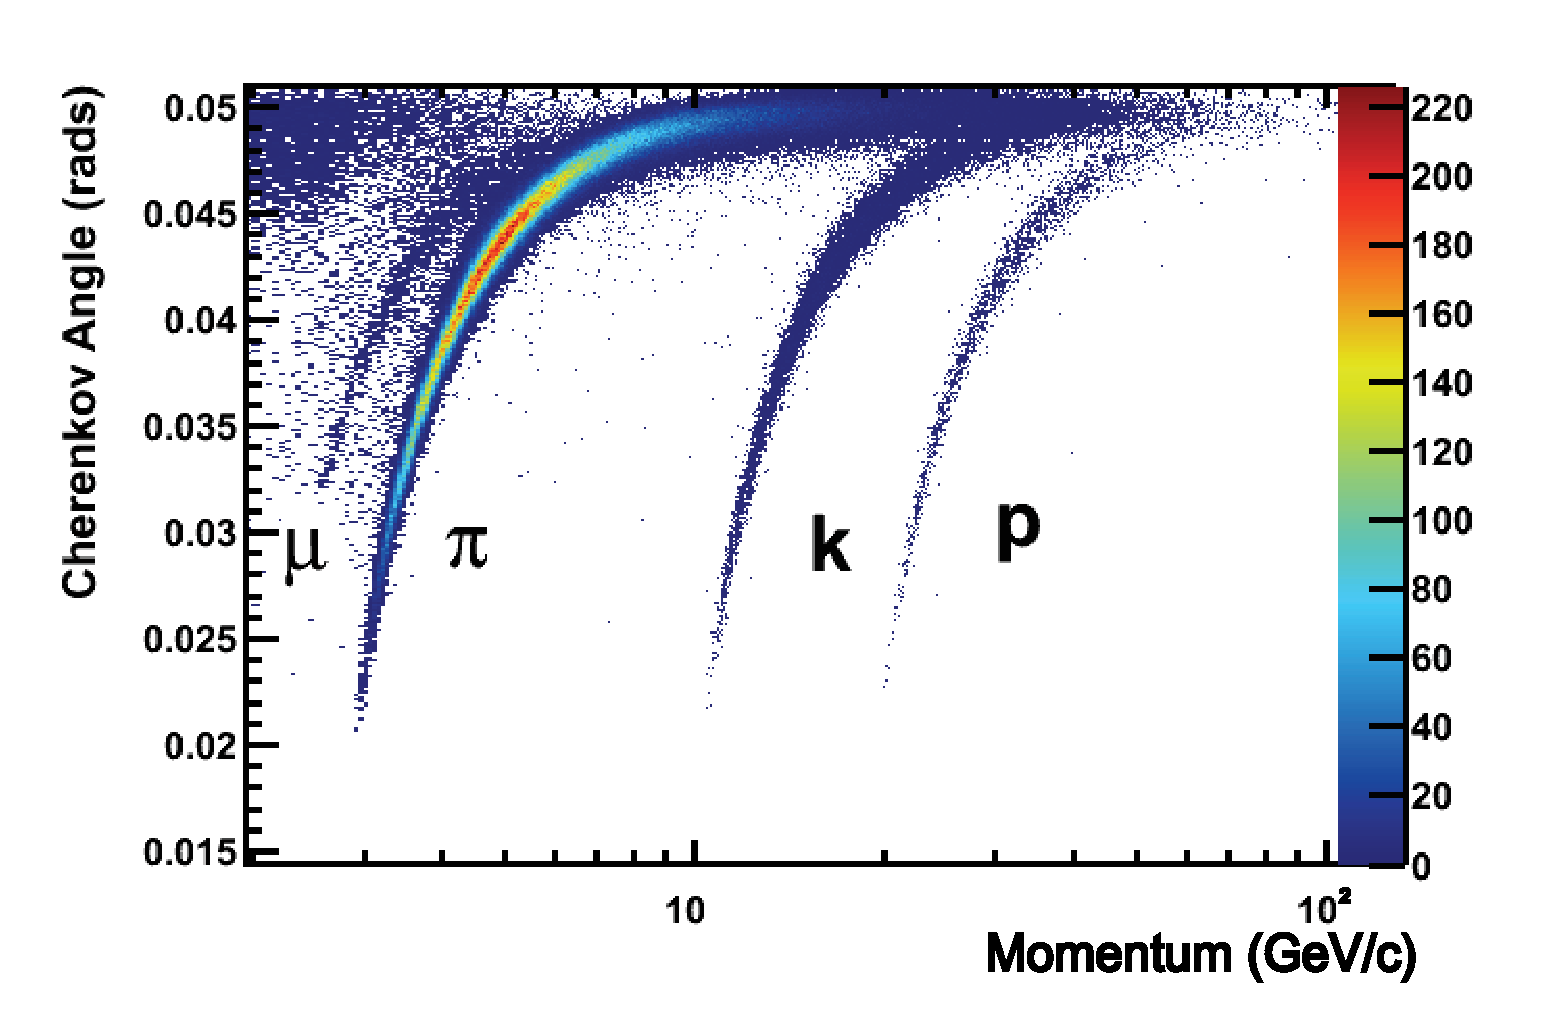
\includegraphics[width = 0.5\textwidth]{figs/detector/CKAnglevsMom_NoTheory_jun2011-01.eps}\put(-50,170){(a)}%
	%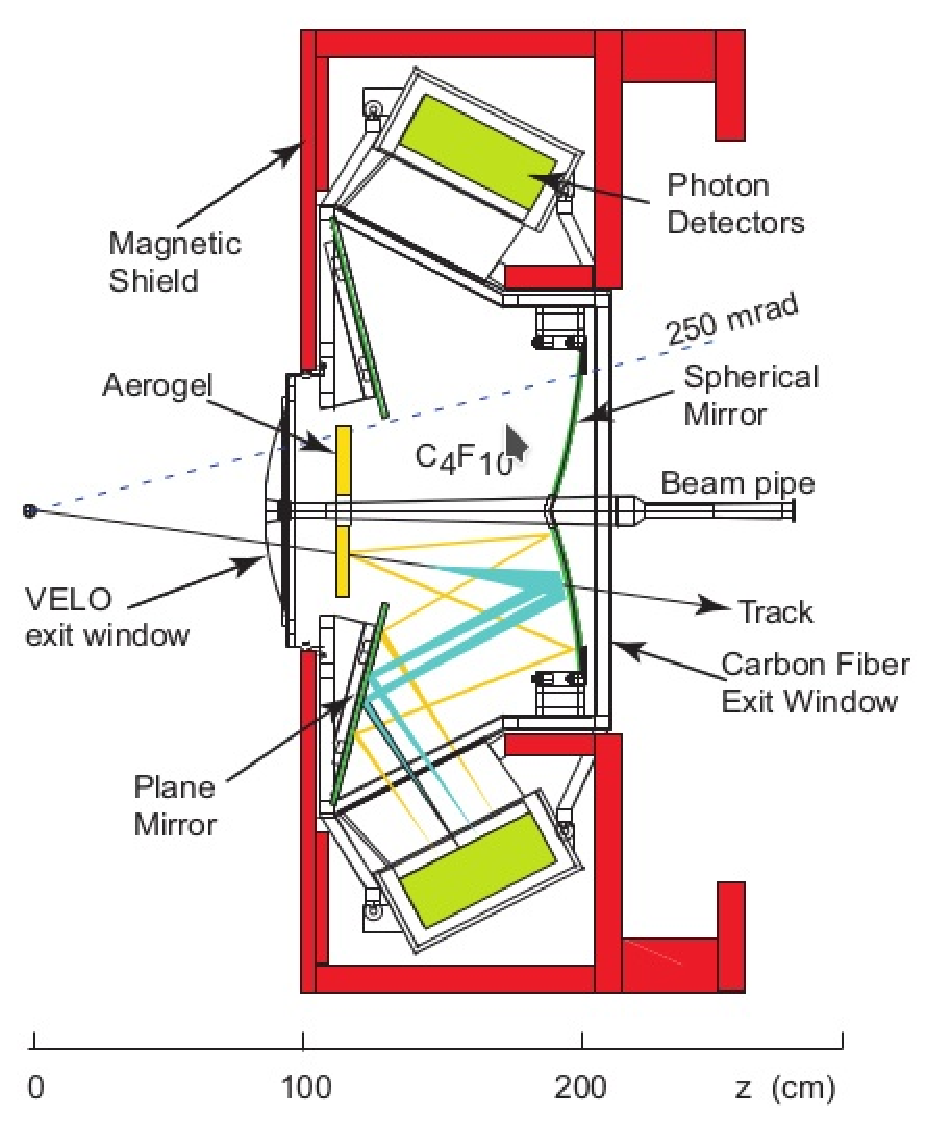
\includegraphics[width = 0.4\textwidth]{figs/detector/mechrich.eps}%
	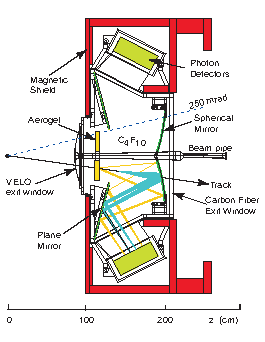
\includegraphics[width = 0.4\textwidth]{figs/detector/license/Rich_croped.pdf}\put(-10,170){(b)}%
	\caption{ (a) Separation power for different species of particles in \DIFaddbeginFL \DIFaddFL{the }\DIFaddendFL momentum-\v{C}erenkov angle plane for \DIFaddbeginFL \DIFaddFL{the }\DIFaddendFL $\rm{C_{4}F_{10}}$ radiator. Figure from \cite{LHCb-DP-2012-003}. (b) Schematic diagram of \gls{RICH1} layout. Figure from \cite{det_paper}.}
	\label{fig:richres}
\end{figure}

\section{RICH Reconstruction and Performance }
In order to \DIFdelbegin \DIFdel{establish }\DIFdelend \DIFaddbegin \DIFadd{correctly associate }\DIFaddend species of particles \DIFdelbegin \DIFdel{for each }\DIFdelend \DIFaddbegin \DIFadd{to a given }\DIFaddend track, the \v{C}erenkov angle is combined with the track momentum measured by tracking. In practice, however, as \Gls{RICH} detectors operate in high track density environment, many \v{C}erenkov rings will be overlapping and hence a complex pattern recognition algorithm is deployed \cite{Forty:1999sg}. 


For each event, the \Gls{RICH} computes a full event likelihood that is consistent with assigning a pion mass hypothesis to all tracks given the observed hit distribution read out by the \Gls{HPD}s. The algorithm then iterates through all other possible particle species, ($e, \mu, \pi, K,$ proton, deuteron), assigning a new full event likelihood for a given track, \DIFdelbegin \DIFdel{having }\DIFdelend \DIFaddbegin \DIFadd{with }\DIFaddend all other hypotheses fixed. The mass hypothesis with the highest full event likelihood is assigned to the track and this process is repeated for all the tracks in the event, until no improvement is found. 

Results of this algorithm provide likelihood variables, $\rm{\textrm{DLL{x}}}$, that quantify the strength of the chosen species hypothesis against the pion hypothesis,
\begin{equation}
	\textrm{\textrm{DLL{x}}} = \mathrm{log}(\mathcal{L})_{x} - \mathrm{log}(\mathcal{L})_{\pi} \quad  x\in{e, \mu, K, \rm{proton, deuteron}}.
\end{equation}

By calculating $\rm{DLL{x_{1}} - DLL{x_{2}}}$, one can obtain discriminative strength between any two species.

\subsection{RICH Performance}
\label{RICHperf}
In order to measure the performance of the \Gls{PID} computed by a \gls{RICH}, populous calibration samples with very little background contamination are required. In order not to bias results, these samples have no \Gls{PID} constraints themselves and are reconstructed solely using kinematic information. For studies of pion/kaon efficiencies, $D^{*+} \to D^{0}(\kaon^{-}\pip)\pip$ backround-substracted samples are used, whereby the daughter tracks of \DIFaddbegin \DIFadd{the }\DIFaddend $D^{0}$ become proxies for the evaluation. The invariant mass for the $D^{0}$ candidates can be seen in~\autoref{fig:richperf}(a)\DIFaddbegin \DIFadd{. }\DIFaddend The probability of correctly identifying a kaon given a certain constraint on $\textrm{DLL{K}}$, \DIFaddbegin \DIFadd{the }\DIFaddend identification efficiency (\Gls{ID}), and \DIFaddbegin \DIFadd{the }\DIFaddend probability of mistakenly swapping pion identification, \DIFaddbegin \DIFadd{the }\DIFaddend misidentification efficiency (\gls{misID}), are summarized in~\autoref{fig:richperf}(b). Identification probabilities of $\approx$ 85\% with \DIFaddbegin \DIFadd{a }\DIFaddend misID rate of $\approx$ 3\% provide invaluable discriminating separation between kaons and pions.




\begin{figure}[!h]
	\centering
	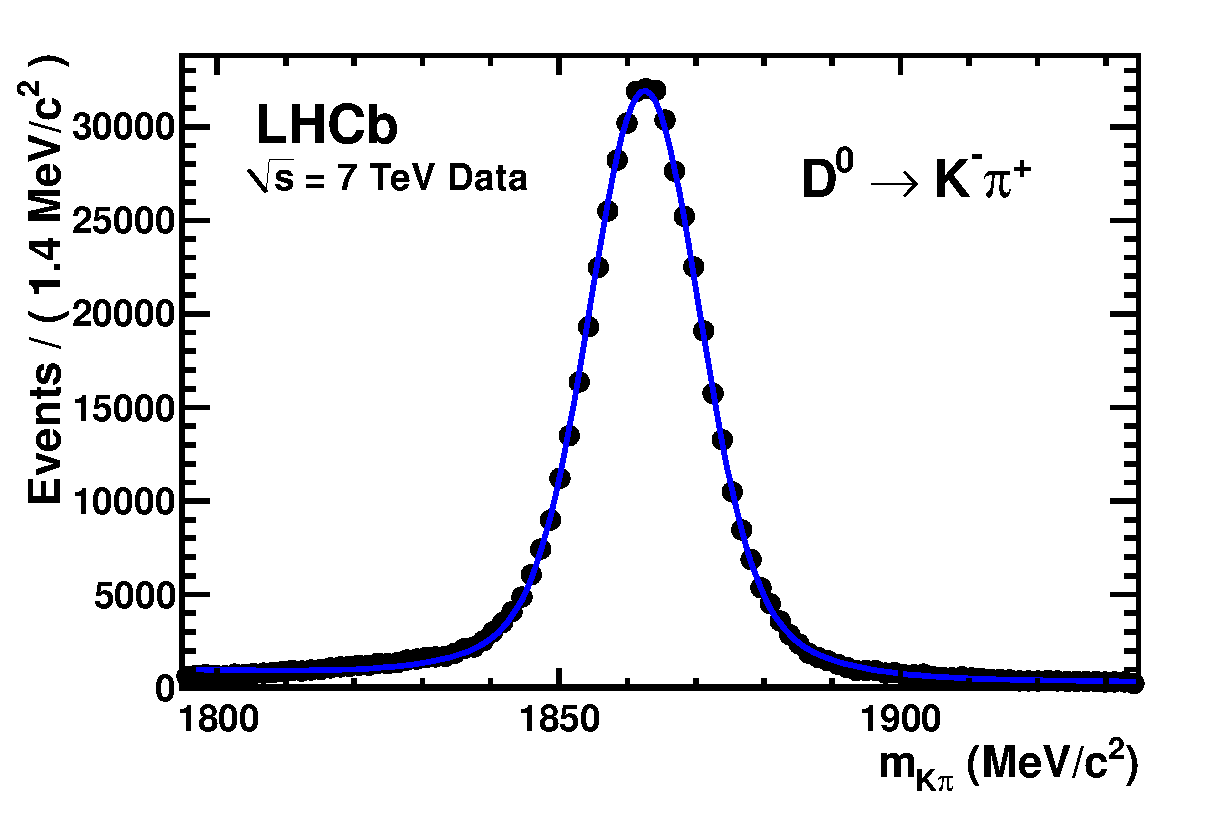
\includegraphics[width = 0.525\textwidth]{figs/detector/D0_Mass.eps}\put(-50,80){(a)}%
	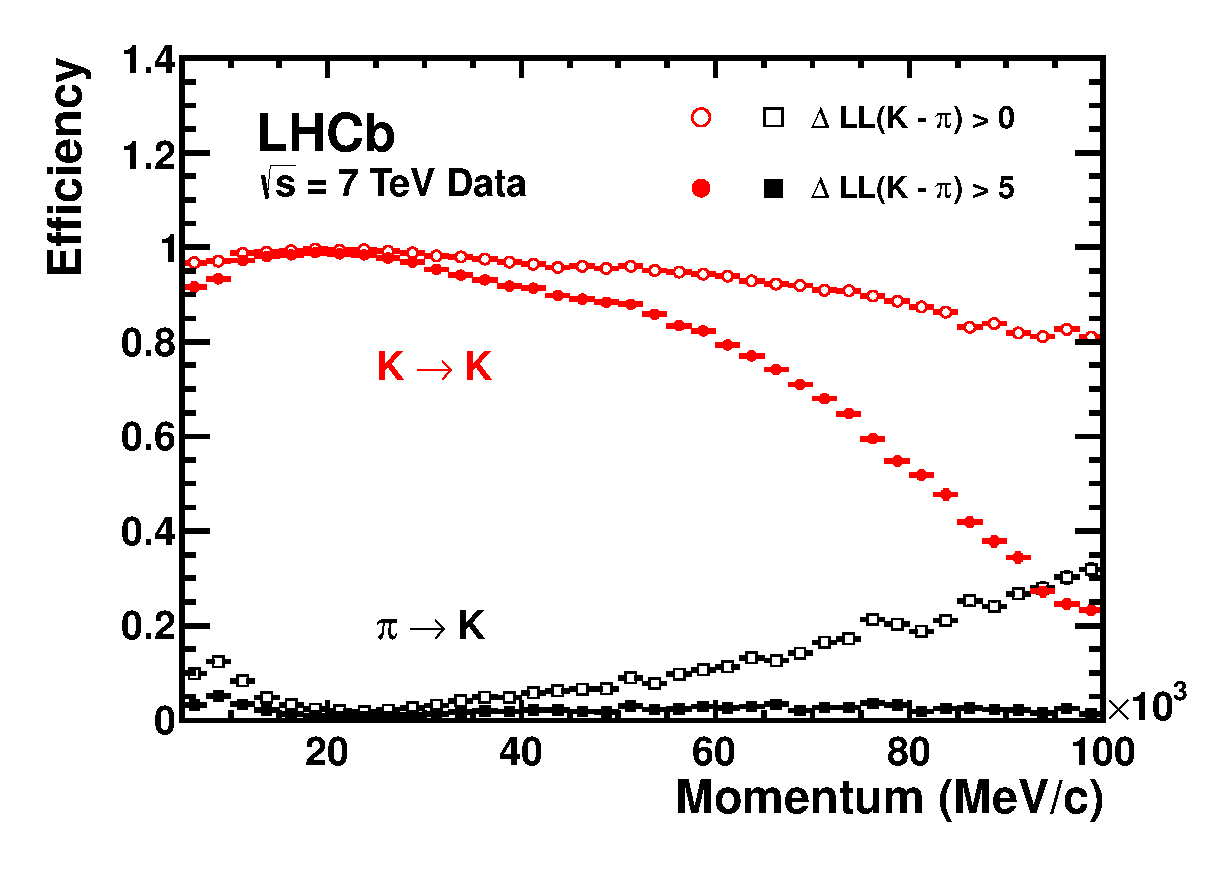
\includegraphics[width = 0.5\textwidth]{figs/detector/KandPi_2_K.eps}\put(-50,80){(b)}%
	\caption{ (a) Invariant mass distribution of $D^{0}$ data sample (in black) overlaid with fit to both background and signal (in blue). (b) An example of kaon ID (red) and misID (black) efficiency as a function of momentum under two \gls{PID} hypotheses, $\textrm{DLL{K}} > 0$ (empty)  and $\textrm{DLL{K}} > 5$ (filled). Both Figures from \cite{LHCb-DP-2012-003}.}
	\label{fig:richperf}
\end{figure}

%In search for $B^{0}$ and $B^{0}_{s}$ decaying to $h^{+}h^{-}$, where $h\in K, \pi$, $\pi^{+} \pi^{-}$ invariant mass spectra with and without \gls{PID} $\textrm{DLL{x}}$ requirements can be seen in~\autoref{fig:richnice}. These plots clearly demonstrate increase in sensitivity searching for $B^{0} \rightarrow \pi^{+} \pi^{-}$ signal amongst other components. 

%\begin{figure}[!h]
%	\centering
%	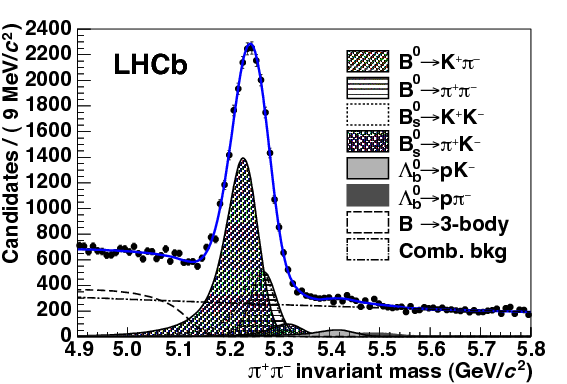
\includegraphics[width = 0.5\textwidth]{figs/detector/b2hhnopid.png}%
%	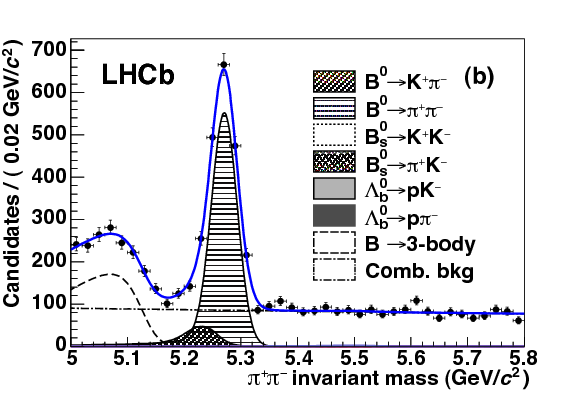
\includegraphics[width = 0.5\textwidth]{figs/detector/b2hhpid.png}%
%	\caption{ $\pi^{+} \pi^{-}$ invariant mass distributions obtained using kinematic constraints only (left) and also using \gls{PID} constraints (right) in order to isolate $B^{0} \rightarrow \pi^{+} \pi^{-}$ peak. This figure is taken from \cite{LHCb-PAPER-2012-002}. }  
%	\label{fig:richnice}
%\end{figure}


\section{Calorimetry }
\label{calosys}
As many other particle physics detectors, \Gls{LHCb} is equipped with series of subdetectors providing separation between electrons, pions and photons. This separation is achieved because different particles interact differently with the material, producing differently shaped showers. This part of the detector is not only integral to the way the \Gls{LHCb} trigger system works but it also provides a measurement of \DIFaddbegin \DIFadd{the }\DIFaddend energies of these objects.
All the subcomponents discussed here operate on the same principle. \DIFdelbegin \DIFdel{Passing particles }\DIFdelend \DIFaddbegin \DIFadd{Particles passing }\DIFaddend through the material emit light. The light from the scintillating material, which is created by absorbing the energy of the \DIFdelbegin \DIFdel{passing }\DIFdelend particle and re-emitted it in \DIFaddbegin \DIFadd{the }\DIFaddend form of light, is guided to photomultiplier tubes by wavelength shifting fibres.

Electrons, pions and photons firstly encounter two planes of scintillating tiles: the Scintillating Pad Detector (\Gls{SPD}), and the Preshower Detector (\Gls{PRS}) intersected by a wall of lead. The \Gls{SPD} senses the passage of charged particles as they emit light whereas neutral particles do not, making this subdetector \DIFaddbegin \DIFadd{able to }\DIFaddend distinguish between electrons and photons. The wall of lead initiates the electromagnetic shower, where photons are converted into electron-positron pairs, depositing sizable energy in the \Gls{PRS} allowing electron/pion separation. 

The Electromagnetic Calorimeter (\Gls{ECAL}) in \gls{LHCb} is based on a sampling shashlik-type technology, where scintillating tiles are alternated \DIFdelbegin \DIFdel{by }\DIFdelend \DIFaddbegin \DIFadd{with }\DIFaddend lead plates measuring the energy deposit of electromagnetic showers. As the best energy resolution requires full energy deposit of energetic photons along the \Gls{ECAL}, the thickness is equivalent to 25 radiation lengths. The resulting resolution of the \Gls{ECAL} is $\frac{\sigma_{E}}{E} = \frac{10\%}{\sqrt{E}} \oplus 1\%$, where $E$ is in \gev.

On the other hand, the Hadronic Calorimeter \Gls{HCAL} sandwiches iron instead of lead as the absorber with \DIFaddbegin \DIFadd{a }\DIFaddend thickness of 5.6 interaction length only, achieving a resolution of $\frac{\sigma_{E}}{E} = \frac{70\%}{\sqrt{E}} \oplus 10\%$ in beam tests. This poorer resolution however fulfils the requirements necessary for the main purpose of this detector, which is the hadron trigger. Away from the beampipe the granularity of cells is coarser to mirror the track occupancy as seen in~\autoref{fig:CaloGran}(a)(b). 

\begin{figure}[!h]
	\centering
	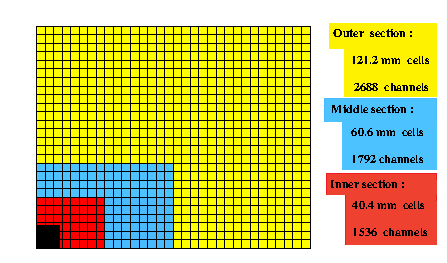
\includegraphics[width = 0.5\textwidth]{figs/detector/license/ECAL_crop.pdf}\put(-70,10){(a)}%%
	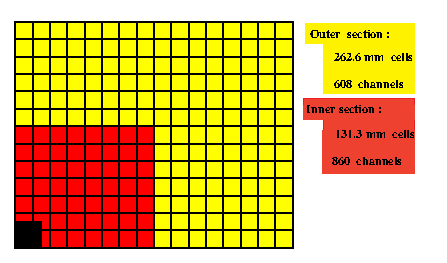
\includegraphics[width = 0.5\textwidth]{figs/detector/license/HCAL_crop.pdf}\put(-70,10){(b)}%%
	\caption{Granularity of (a) \Gls{ECAL} and (b) \Gls{HCAL} detectors. This is just a quarter view and that the black region is where the beam pipe is located. Figure from \cite{det_paper}. }  
	\label{fig:CaloGran}
\end{figure}




\section{Muon Stations }
\label{muonsys}
Muons are considered to be of fundamental importance to many flagship analyses by \Gls{LHCb}, such as the search for the rare $\B^{0}_{s} \rightarrow \mu^{+} \mu^{-}$ decay\cite{Aaij:2017vad}. Analysis of \Bmumumu of course relies heavily on \DIFaddbegin \DIFadd{a }\DIFaddend good performance of this part of \DIFaddbegin \DIFadd{the }\DIFaddend detector. Muon stations are positioned at the end of the detector, taking advantage of the fact that muons penetrate material better than any other particle type. 

\Gls{LHCb}'s five rectangular muon stations \Gls{muonstation} are positioned before and after \DIFaddbegin \DIFadd{the }\DIFaddend calorimetry system, with \DIFaddbegin \DIFadd{the }\DIFaddend first station M1 upstream of the \Gls{SPD}, and four stations (M2-M5) downstream of \Gls{HCAL} as shown in~\autoref{fig:MuonGran}. The M1 station consists of 12 sets of three gas electron 
multiplier foils (triple-GEMs) in the region closest to the beam pipe, resisting the highest dose of radiation due to the highest particle flux. Its main use lies in improving the measurement of $p_{T}$ in the hardware trigger. The M2-M5 stations each consist of 276 multi-wire proportional chambers (\Gls{MWPCs}) filled with an $\rm{Ar,CO_{2},CF_{4}}$ gas mixture. They are interlayered with 0.8\m iron walls, to provide a stopping target for all particles, other than muons with momentum higher than $6$ \gevc.

%In order to ease the accessibility, like in \Gls{VELO}, all the stations are split into two independent mechanical sides, also known A and C side.

Each half of a muon station is segmented into four increasingly larger regions away from the beam, R1 to R4.
 All the regions were constructed to cover the same acceptance, keeping the track occupancy constant across the station. The granularity of the readout is higher in the horizontal plane to take advantage of the magnet's horizontal bending plane.




\begin{figure}[!h]
	\centering
	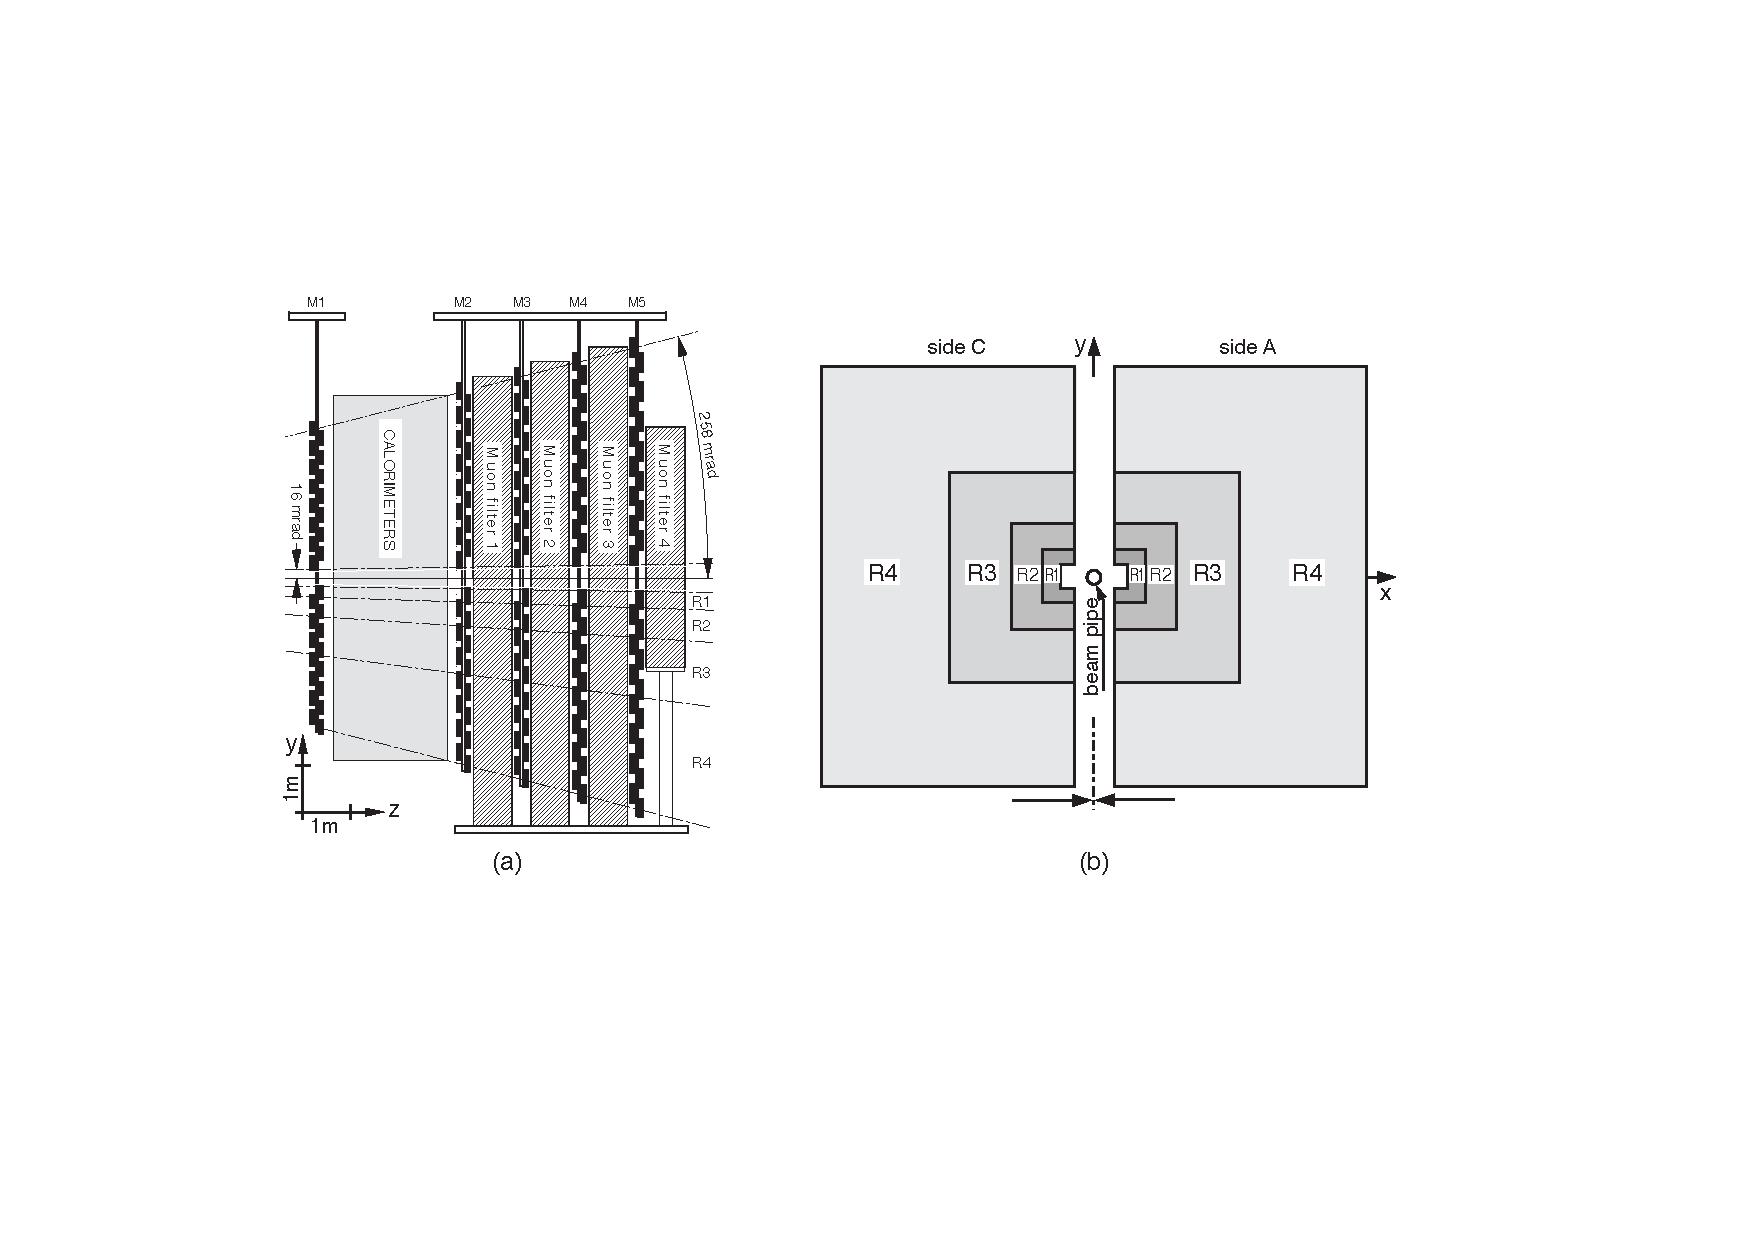
\includegraphics[width = 1.0\textwidth]{figs/detector/sideview.pdf}%
	%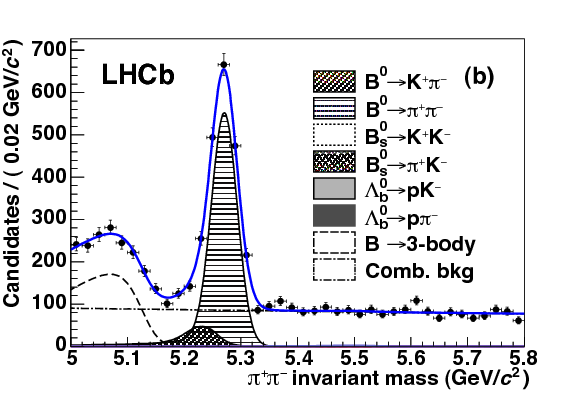
\includegraphics[width = 0.5\textwidth]{figs/detector/b2hhpid.png}%
	\caption{(a) Layout of the muon detector x-z plane and (b) x-y plane. Figure from \cite{LHCb-DP-2012-002}. }  
	\label{fig:MuonGran}
\end{figure}

Both GEM and \Gls{MWPCs} operate on \DIFdelbegin \DIFdel{a }\DIFdelend \DIFaddbegin \DIFadd{the }\DIFaddend same principle. In each station, the position in the $x-y$ plane is determined by ionizing electrons that come from muons passing through the detector, which are then attracted either to the closest anode mesh or wire mesh. The trigger is fired if the corresponding rectangular region in each station registered a positive binary decision. This means \DIFdelbegin \DIFdel{an }\DIFdelend \DIFaddbegin \DIFadd{the }\DIFaddend efficiency of each station must be $\geq$99\% to give \DIFaddbegin \DIFadd{an }\DIFaddend overall 95\% trigger efficiency. %Geometrical layout covers $\approx$ 20\% muons originating in semileptonic $b$ decays.\mybox{\color{red}CERN-THESIS-2012-025.pdf from puig, i have to invedtigate}


\subsection{Muon Identification }
\label{muonID}
Apart from triggering events with high enough $p_{T}$ muons, the muon stations provide necessary \gls{PID} information for muon analyses. Offline variables mostly used for muon ID by analysts are
 \begin{itemize} 
	\DIFdelbegin %DIFDELCMD < \item{\textbf{IsMuon}: Boolean decision of muon candidates with momentum-dependent categorisation. Long tracks with $p>3$\gev/c are extrapolated to muon stations yielding $x-y$ coordinates in M2-M5, considering only tracks within acceptance. For each station, a search for hit information within an elliptical area defined by momentum, a field of interest (\Gls{FOI}), is performed. The hit requirements are summarized in~\autoref{tab:ismuontab}.}
%DIFDELCMD < 	\item{\textbf{muDLL}: Difference in log likelihoods computed using muon and non-muon hypothesis. These hypotheses are based on the proximity/distance $D^{2}$ of the track extrapolation into the muon stations and corresponding closest sensed hits in those stations. Muon-like particle will tend to have sharper distribution in $D^{2}$ as compared to other species. Protons were chosen to be the other species for the calibration purposes. They give a broader distribution as they originate either as punch-through protons (protons coming from showers not fully contained in the \gls{HCAL}), protons having coincident hit position to a true muon, or random hits.}
%DIFDELCMD < 	%%%
\DIFdelend \DIFaddbegin \item{\textbf{IsMuon}: Boolean decision of muon candidates with momentum-dependent categorisation. Long tracks with $p>3$\gev/c are extrapolated to muon stations yielding $x-y$ coordinates in M2-M5, considering only tracks within the acceptance. For each station, a search for hit information within an elliptical area defined by momentum, a field of interest (\Gls{FOI}), is performed. The hit requirements are summarized in~\autoref{tab:ismuontab}.}
	\item{\textbf{muDLL}: Difference in log likelihoods computed using a muon and non-muon hypothesis. These hypotheses are based on the prox imity/distance, $D^{2}$, of the track extrapolation into the muon stations and corresponding closest sensed hits in those stations. Muon-like particles will tend to have a sharper distribution in $D^{2}$ as compared to other species. Protons were chosen to be the other species for the calibration purposes. They give a broader distribution as they originate either as punch-through protons (protons coming from showers not fully contained in the \gls{HCAL}), protons having the same hit position as true muon, or random hits.}
	\DIFaddend \item{\textbf{DLLmu}}:  For each track \DIFdelbegin \DIFdel{a }\DIFdelend \DIFaddbegin \DIFadd{the same }\DIFaddend global likelihood is produced, by \DIFdelbegin \DIFdel{combination of }\DIFdelend \DIFaddbegin \DIFadd{combining the }\DIFaddend muon and non-muon \DIFdelbegin \DIFdel{likelihood }\DIFdelend \DIFaddbegin \DIFadd{likelihoods }\DIFaddend from \textbf{muDLL}, with the \Gls{RICH} different mass hypothesis likelihoods, and \DIFaddbegin \DIFadd{the }\DIFaddend calorimetry likelihood exploiting \DIFaddbegin \DIFadd{information about }\DIFaddend the energy deposits\DIFdelbegin \DIFdel{information}\DIFdelend . Like in the \Gls{RICH} likelihoods, the default hypothesis corresponds to separation between the muon and pion hypotheses.    

 \end{itemize} 

\noindent \DIFdelbegin \DIFdel{Other variables which are extensively used for muon particle identification in }\DIFdelend \DIFaddbegin \DIFadd{In the }\Bmumumu \DIFadd{analysis the variables }\texttt{\DIFadd{IsMuon}} \DIFadd{and }\texttt{\DIFadd{DLLmu}} \DIFadd{are used to identify muons. In addition, other variables that are used for muon identification in the }\DIFaddend search for \Bmumumu\DIFaddbegin \DIFadd{, }\DIFaddend are described in~\autoref{otherpid}. \DIFaddbegin \DIFadd{The use of several variables for muon identification is done as they are mostly complimentary, exploiting different information from different parts of the detector. 
}\DIFaddend 

\begin{table}[!h]
	\centering
	\hspace*{-0.8cm}
	\begin{tabular}{c c}
		\toprule
		Particle Momentum $p$  & Hits in Muon Stations \\ \hline
		3 \gev/c <$p$<6 \gev/c & M1 $\&$ M2\\
		6 \gev/c <$p$<10 \gev/c & M1 $\&$ M2 $\&$ (M3 $||$ M4) \\
		10 \gev/c <$p$ & M1, M2, M3 and M4 \\ \bottomrule      
	\end{tabular}
	\caption{Momentum-dependent definition \texttt{IsMuon} variable.}
	\label{tab:ismuontab}
\end{table}   

\subsection{Muon Identification Performance}
\label{muonperf}
As for hadron performance measurements, the muon ID performance is determined using the high statistics decay channel $J/\psi \rightarrow \mu^{+} \mu^{-}$ with a \textit{tag and probe} method. MisID rates \DIFdelbegin \DIFdel{of }\DIFdelend \DIFaddbegin \DIFadd{for }\DIFaddend kaons and pions are computed using the same decay channels, which were used for \DIFaddbegin \DIFadd{the }\DIFaddend identification of hadrons, $D^{*+} \to D^{0}(\kaon^{-}\pip)\pip$. The summary of \texttt{IsMuon} ID and misID rates are presented in~\autoref{fig:MuonID}. \DIFdelbegin \DIFdel{Very }\DIFdelend \DIFaddbegin \DIFadd{A very }\DIFaddend high ID rate (above 90\%) for relatively low misID probability (below 10\%) is key to analyses with muons in \DIFdelbegin \DIFdel{a }\DIFdelend \DIFaddbegin \DIFadd{the }\DIFaddend final state. \DIFdelbegin \DIFdel{But the least performing are the }\DIFdelend \DIFaddbegin \DIFadd{The identification rate for the }\DIFaddend low $p_{T}$ muons \DIFdelbegin \DIFdel{where the identification }\DIFdelend suffers because these muons can end up outside of the \gls{LHCb} acceptance\DIFdelbegin \DIFdel{and misID }\DIFdelend \DIFaddbegin \DIFadd{. MisID }\DIFaddend rates for kaon and pions are significantly higher in \DIFaddbegin \DIFadd{the }\DIFaddend low momenta region as the dominant process \DIFdelbegin \DIFdel{causing this are }\DIFdelend \DIFaddbegin \DIFadd{for this occurence is }\DIFaddend muons from decay-in-flight.   

\begin{figure}[!h]
	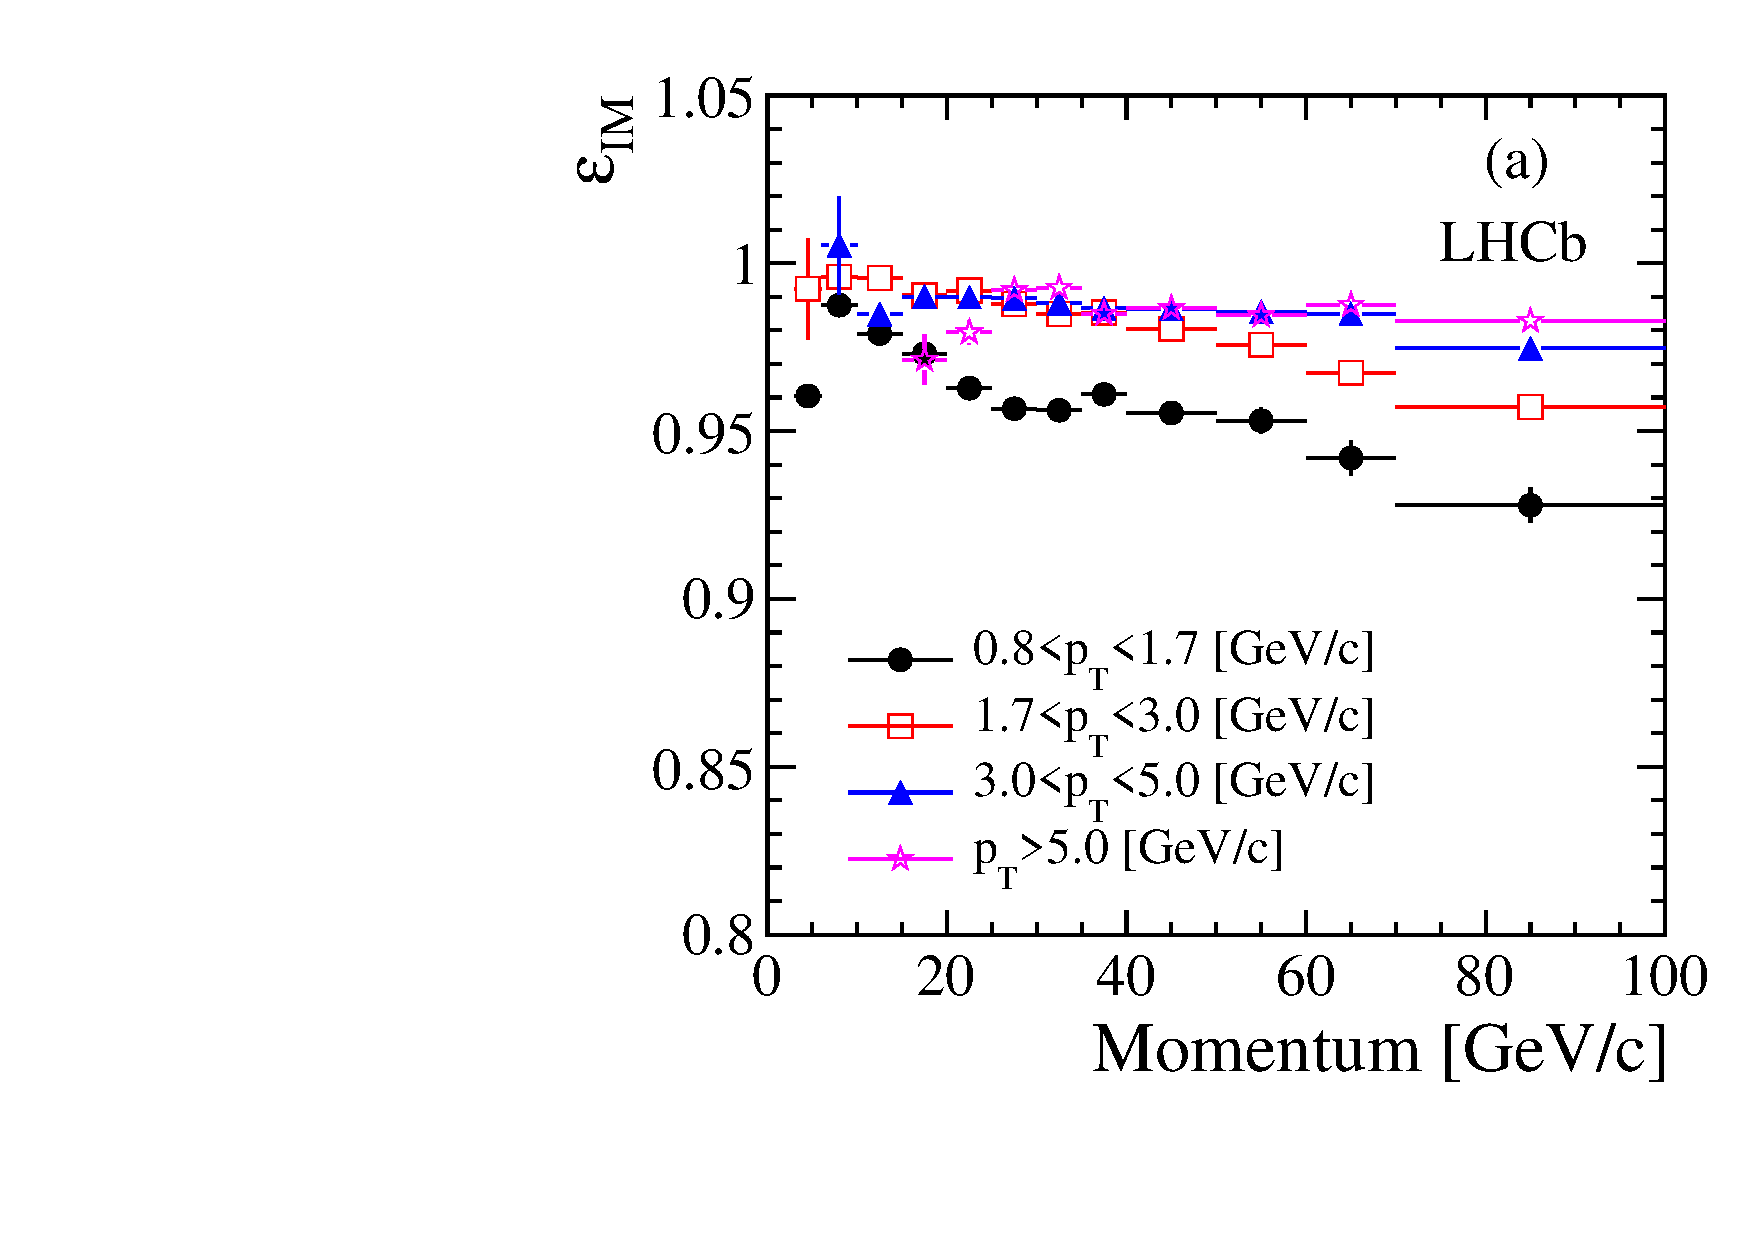
\includegraphics[width = 0.5\textwidth]{figs/detector/dllFit_mu_IMvsPvsPt.pdf}%
	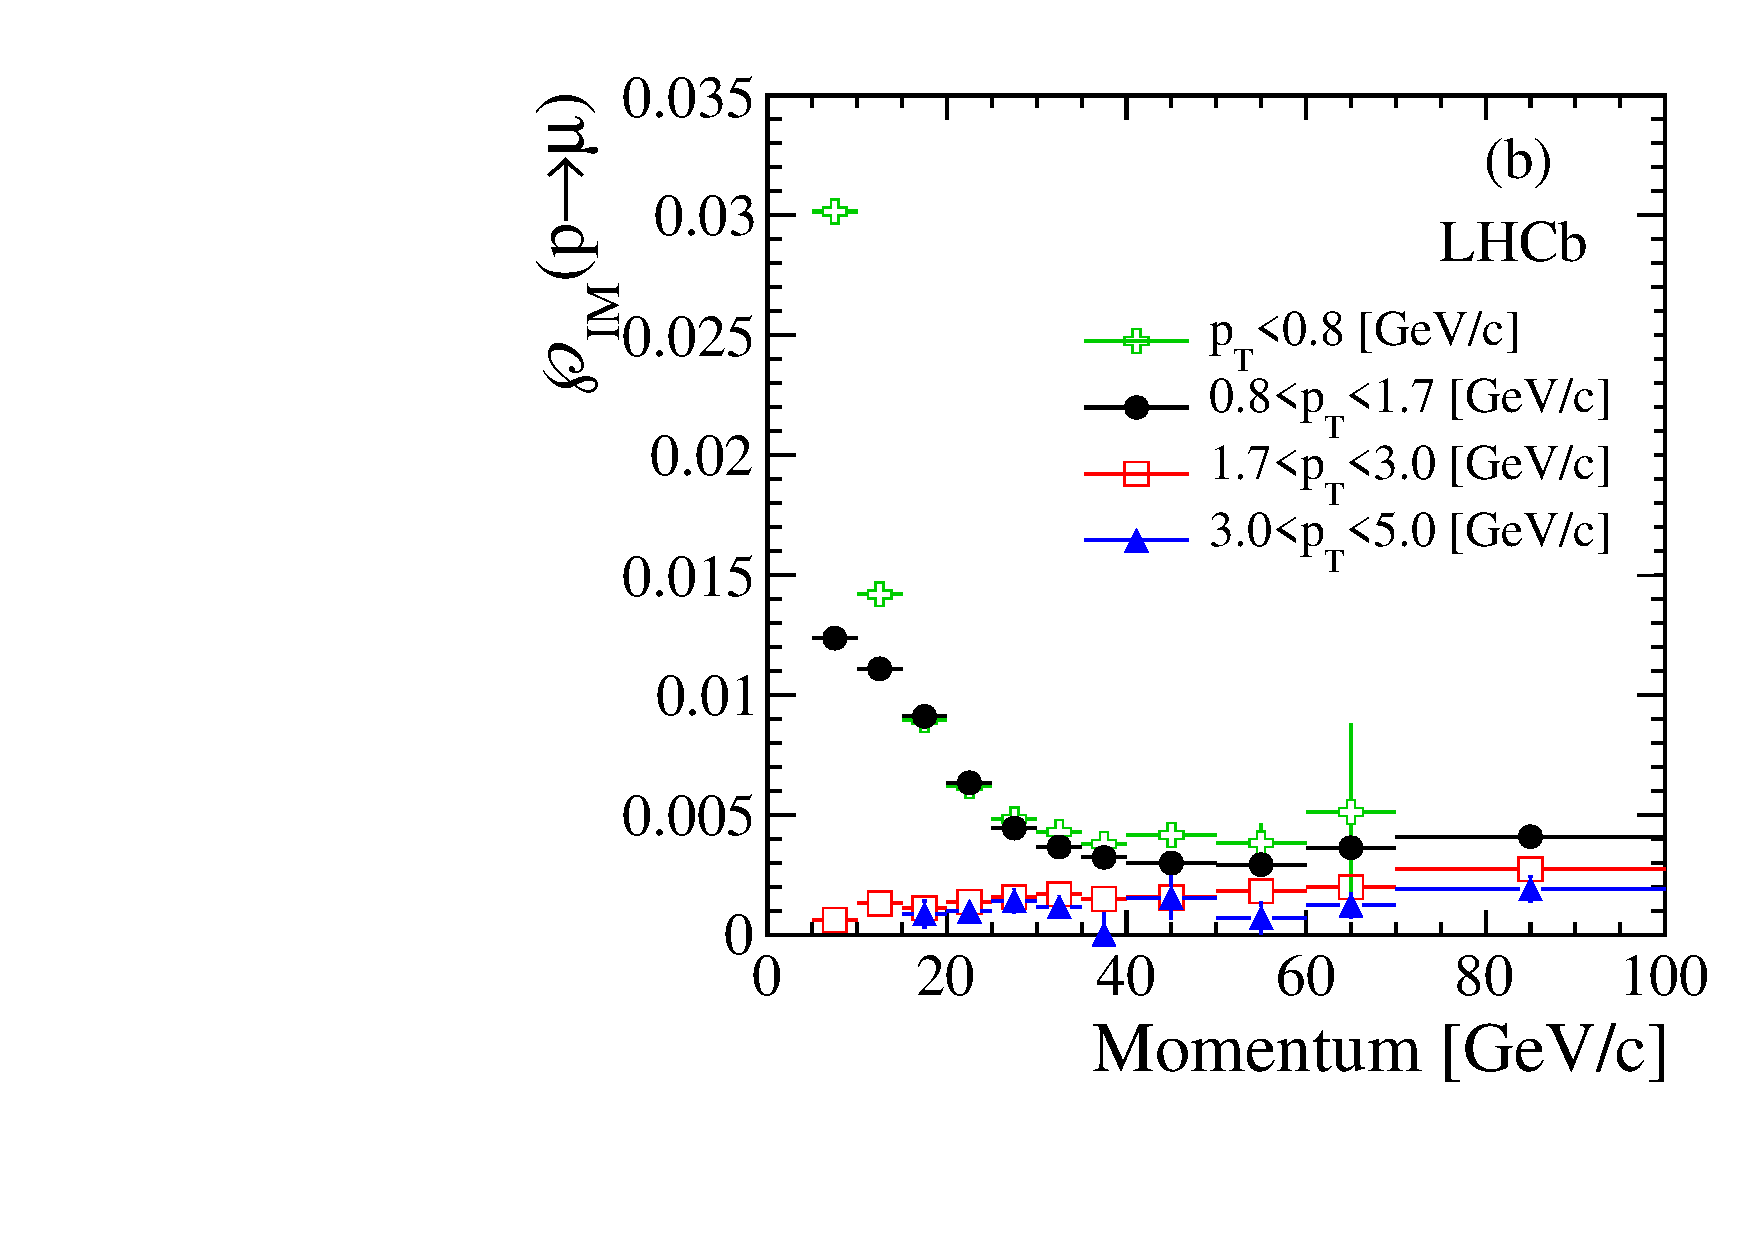
\includegraphics[width = 0.5\textwidth]{figs/detector/dllFit_P_IMvsPvsPt.pdf}%
       \newline
	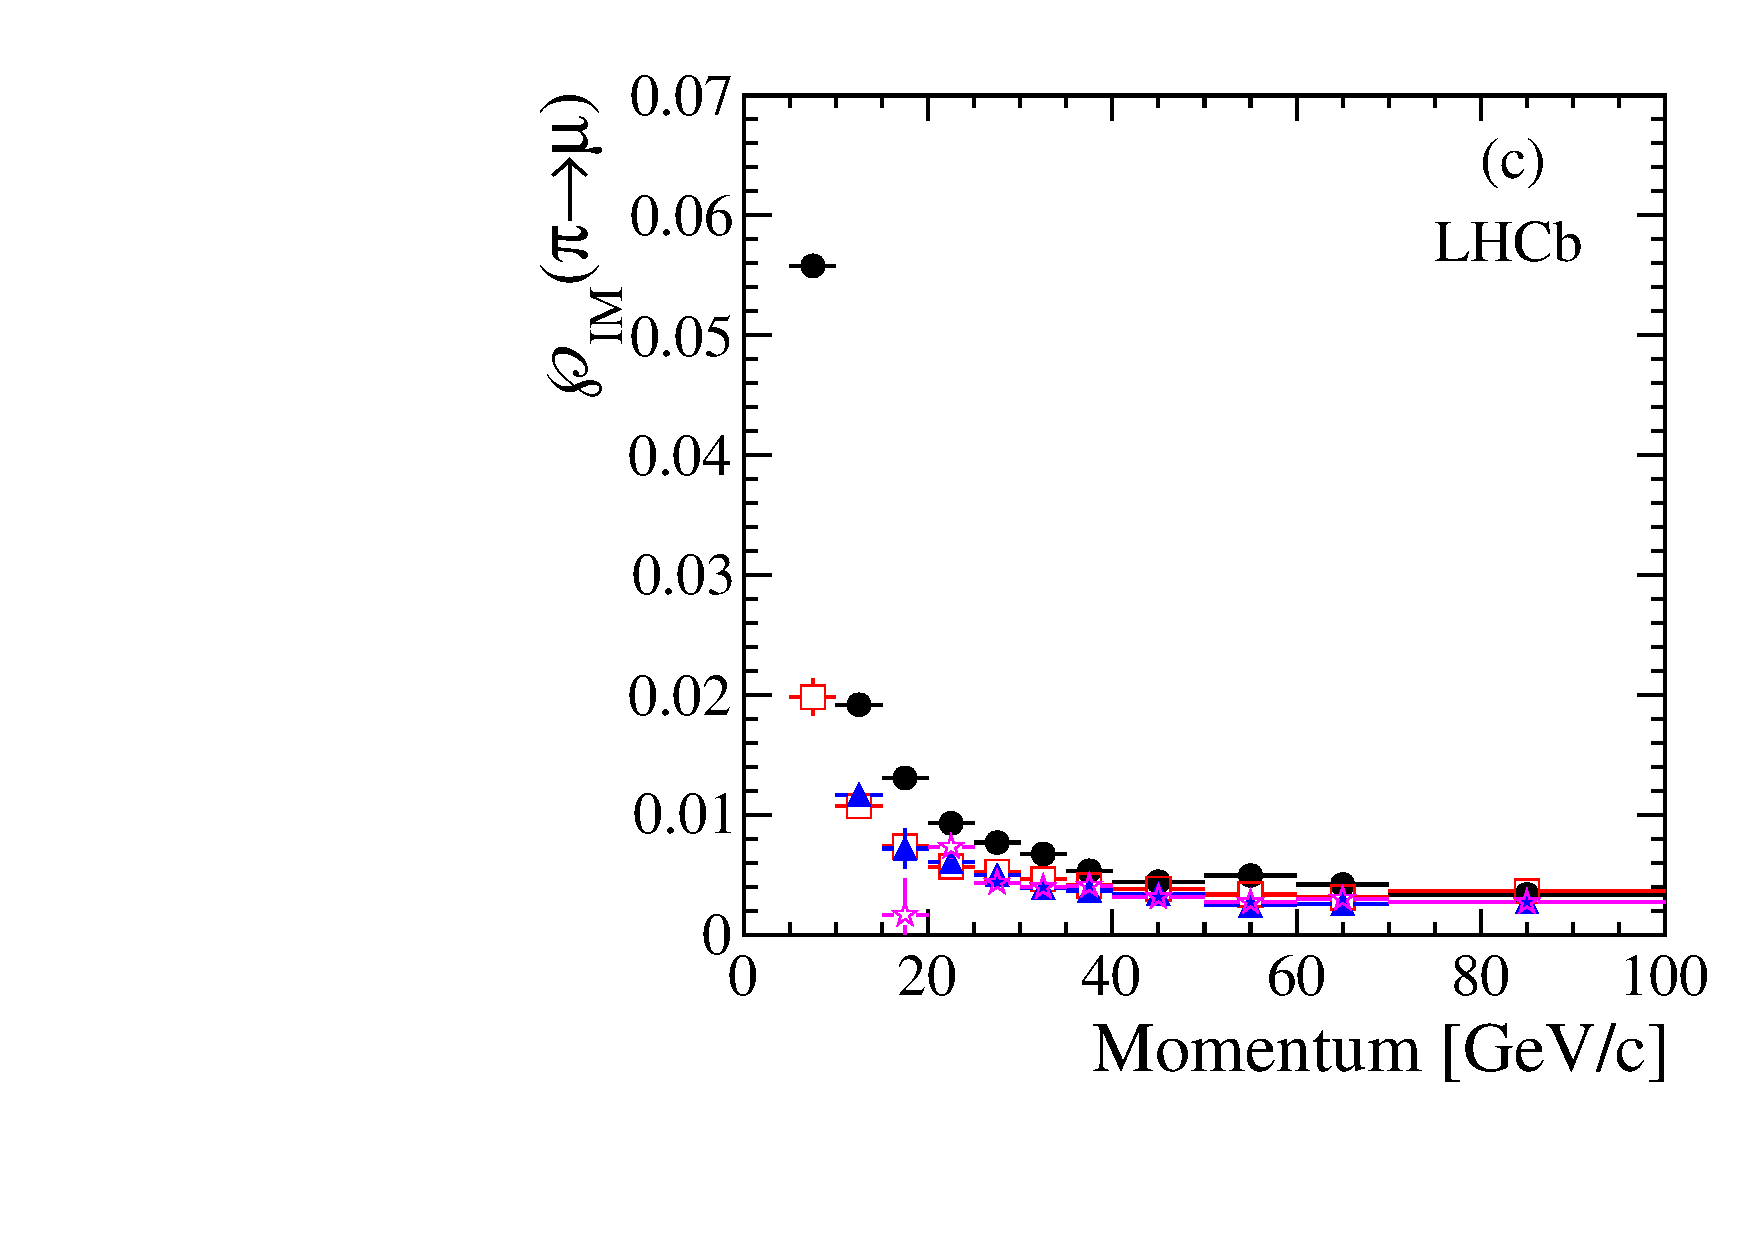
\includegraphics[width = 0.5\textwidth]{figs/detector/dllFit_pi_IMvsPvsPt.pdf}%
	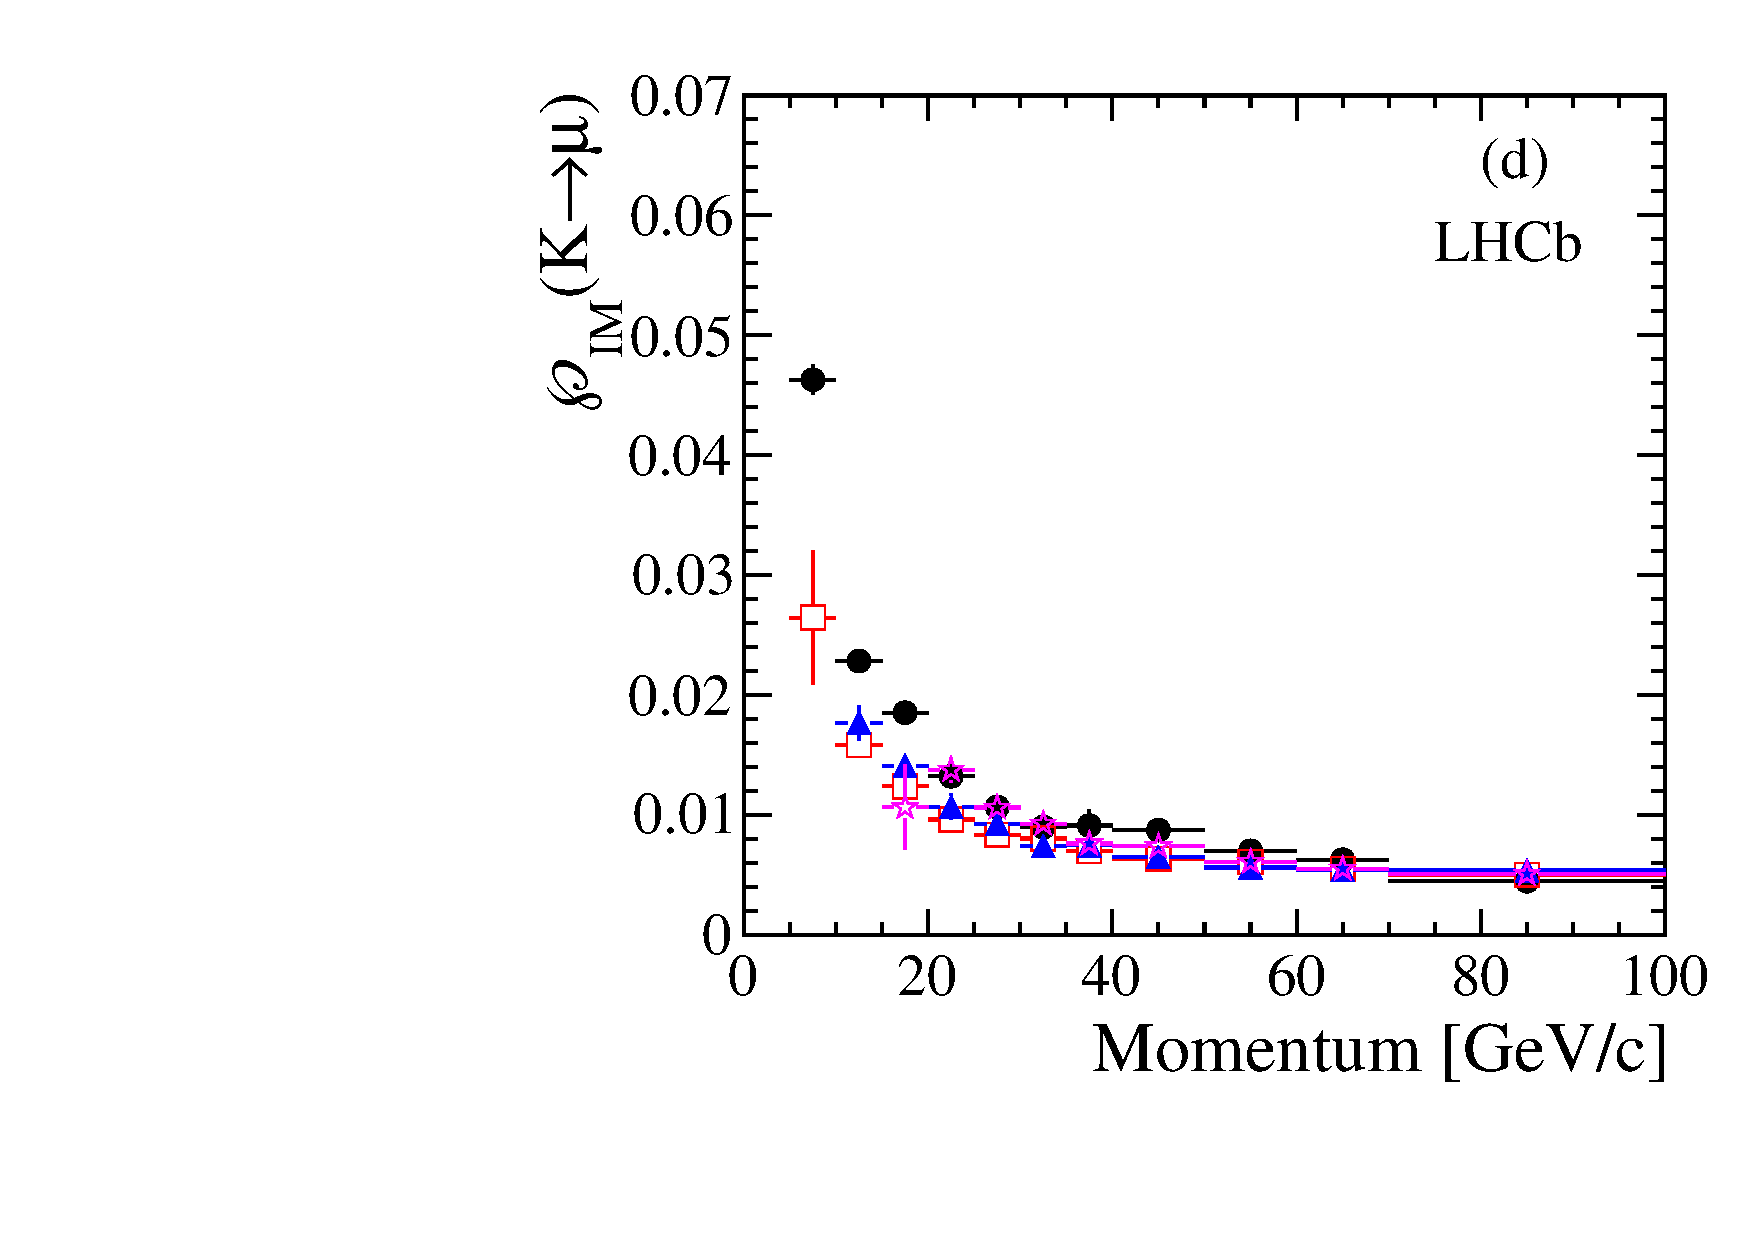
\includegraphics[width = 0.5\textwidth]{figs/detector/dllFit_ka_IMvsPvsPt.pdf}%
	\caption{(a) Probability of correctly identifying muons as a function of momentum \DIFdelbeginFL \DIFdelFL{$p$ }\DIFdelendFL in \DIFdelbeginFL \DIFdelFL{the }\DIFdelendFL bins of $p_{T}$ for $J/\psi \rightarrow \mu^{+} \mu^{-}$ with \DIFaddbeginFL \DIFaddFL{an }\DIFaddendFL \texttt{IsMuon} constraint. (c) Probability of incorrectly identifying \DIFaddbeginFL \DIFaddFL{a }\DIFaddendFL pion (b) proton and (d) kaon as \DIFaddbeginFL \DIFaddFL{a }\DIFaddendFL muon with \texttt{IsMuon}. This figure is taken from \cite{LHCb-DP-2013-001}. }  
	\label{fig:MuonID}
\end{figure}


\section{Trigger }
\label{triggerchap}
Big-data physics experiments have to make decisions on what kind of data they want to keep. The choice of interesting events is performed by a series of decisions, which is known as the trigger. The \Gls{LHCb} trigger system was build around constraints posed by the run conditions, read-out capabilities and available disk space. In Run \Rn{1} and Run \Rn{2} \gls{LHCb} has at its disposal the multistage trigger consisting of a hardware-based level 0 trigger (\Gls{L0}) and a software-based high level trigger (\Gls{HLT}).

In the end, selected events have their trigger decisions categorized. An event where the signal candidate caused the trigger to fire is known \DIFdelbegin \DIFdel{to be }\DIFdelend \DIFaddbegin \DIFadd{as }\DIFaddend Trigger on Signal (\Gls{TOS}). An event where it is a non-signal like particle causing the trigger decision to occur \DIFdelbegin \DIFdel{, }\DIFdelend \DIFaddbegin \DIFadd{is labelled as }\DIFaddend Trigger Independent of Signal (\Gls{TIS})\DIFdelbegin \DIFdel{is labelled}\DIFdelend . Finally, if only \DIFdelbegin \DIFdel{by }\DIFdelend a combination of signal particle(s) together with other \DIFdelbegin \DIFdel{particle's properties }\DIFdelend \DIFaddbegin \DIFadd{particles }\DIFaddend in the event \DIFdelbegin \DIFdel{produce }\DIFdelend \DIFaddbegin \DIFadd{produces }\DIFaddend an affirmative decision, then these events are categorized as \Gls{TIS} $\&$ \Gls{TOS} = \Gls{TISTOS}.

\Gls{L0} reduces the rate of data from 40 \mhz to 1 \mhz by employing five trigger decisions, also known as lines. The first three lines make \DIFaddbegin \DIFadd{a }\DIFaddend decision using calorimeter information about the transverse energy, $E_{T}$, \DIFaddbegin \DIFadd{and }\DIFaddend whether it is \DIFaddbegin \DIFadd{a }\DIFaddend photon, electron or hadron causing the shower energy deposit. Two other lines \DIFdelbegin \DIFdel{are reading }\DIFdelend \DIFaddbegin \DIFadd{read }\DIFaddend out information from the muon system by looking for  \DIFdelbegin \DIFdel{transverse momentum, }\DIFdelend $p_{T}$, of muon and dimuon (two muon tracks) objects. \DIFdelbegin \DIFdel{Efficiencies }\DIFdelend \DIFaddbegin \DIFadd{The efficiencies }\DIFaddend of the L0 muon triggers are evaluated using $B^{+} \rightarrow (J/\psi \rightarrow \mu^{+} \mu^{-}) K^{+}$ decays and can be seen in~\autoref{fig:L0Perf}(a). The hadron trigger efficiency in different decay channels can be seen in~\autoref{fig:L0Perf}(b). 


\begin{figure}[!h]
	\centering
	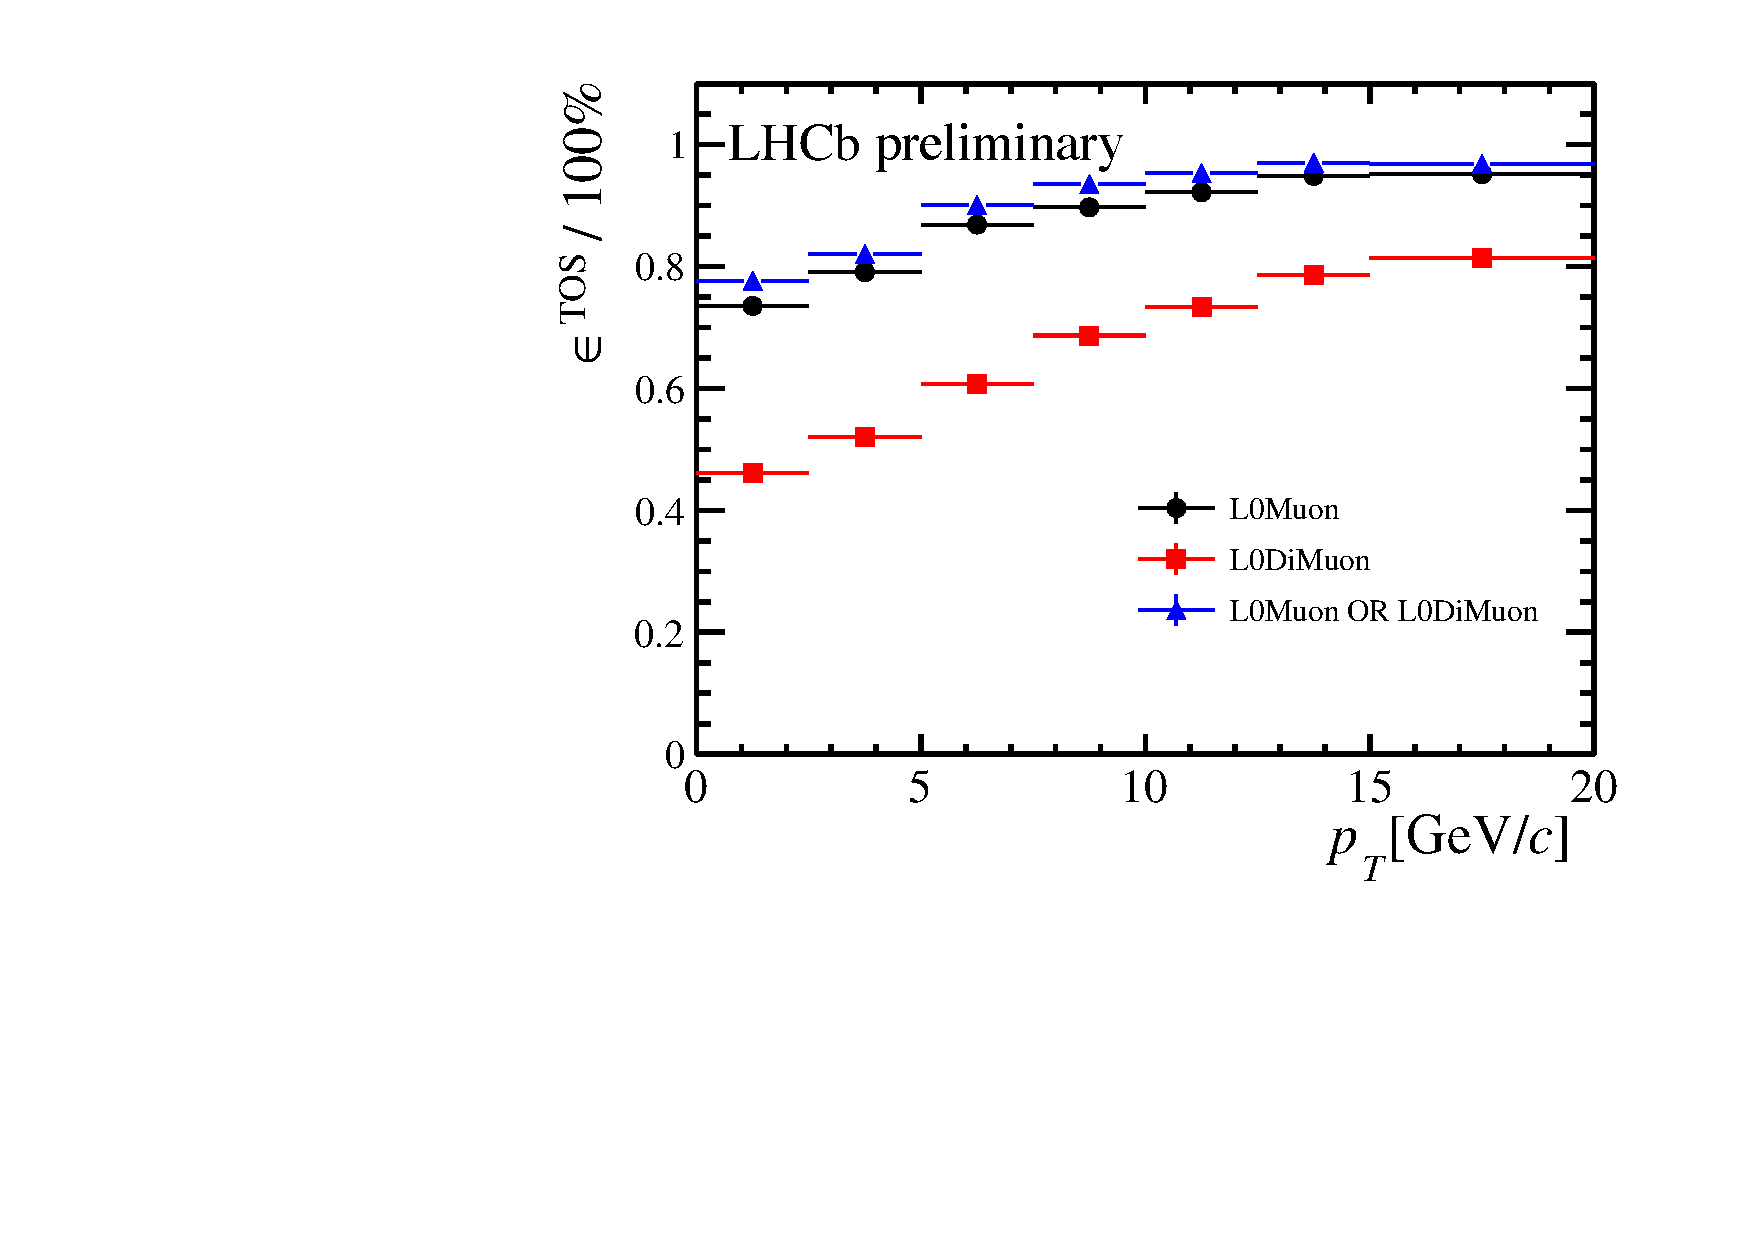
\includegraphics[width = 0.5\textwidth]{figs/detector/Fig1_L0MuonEff_PT.pdf}\put(-50,90){(a)}%
	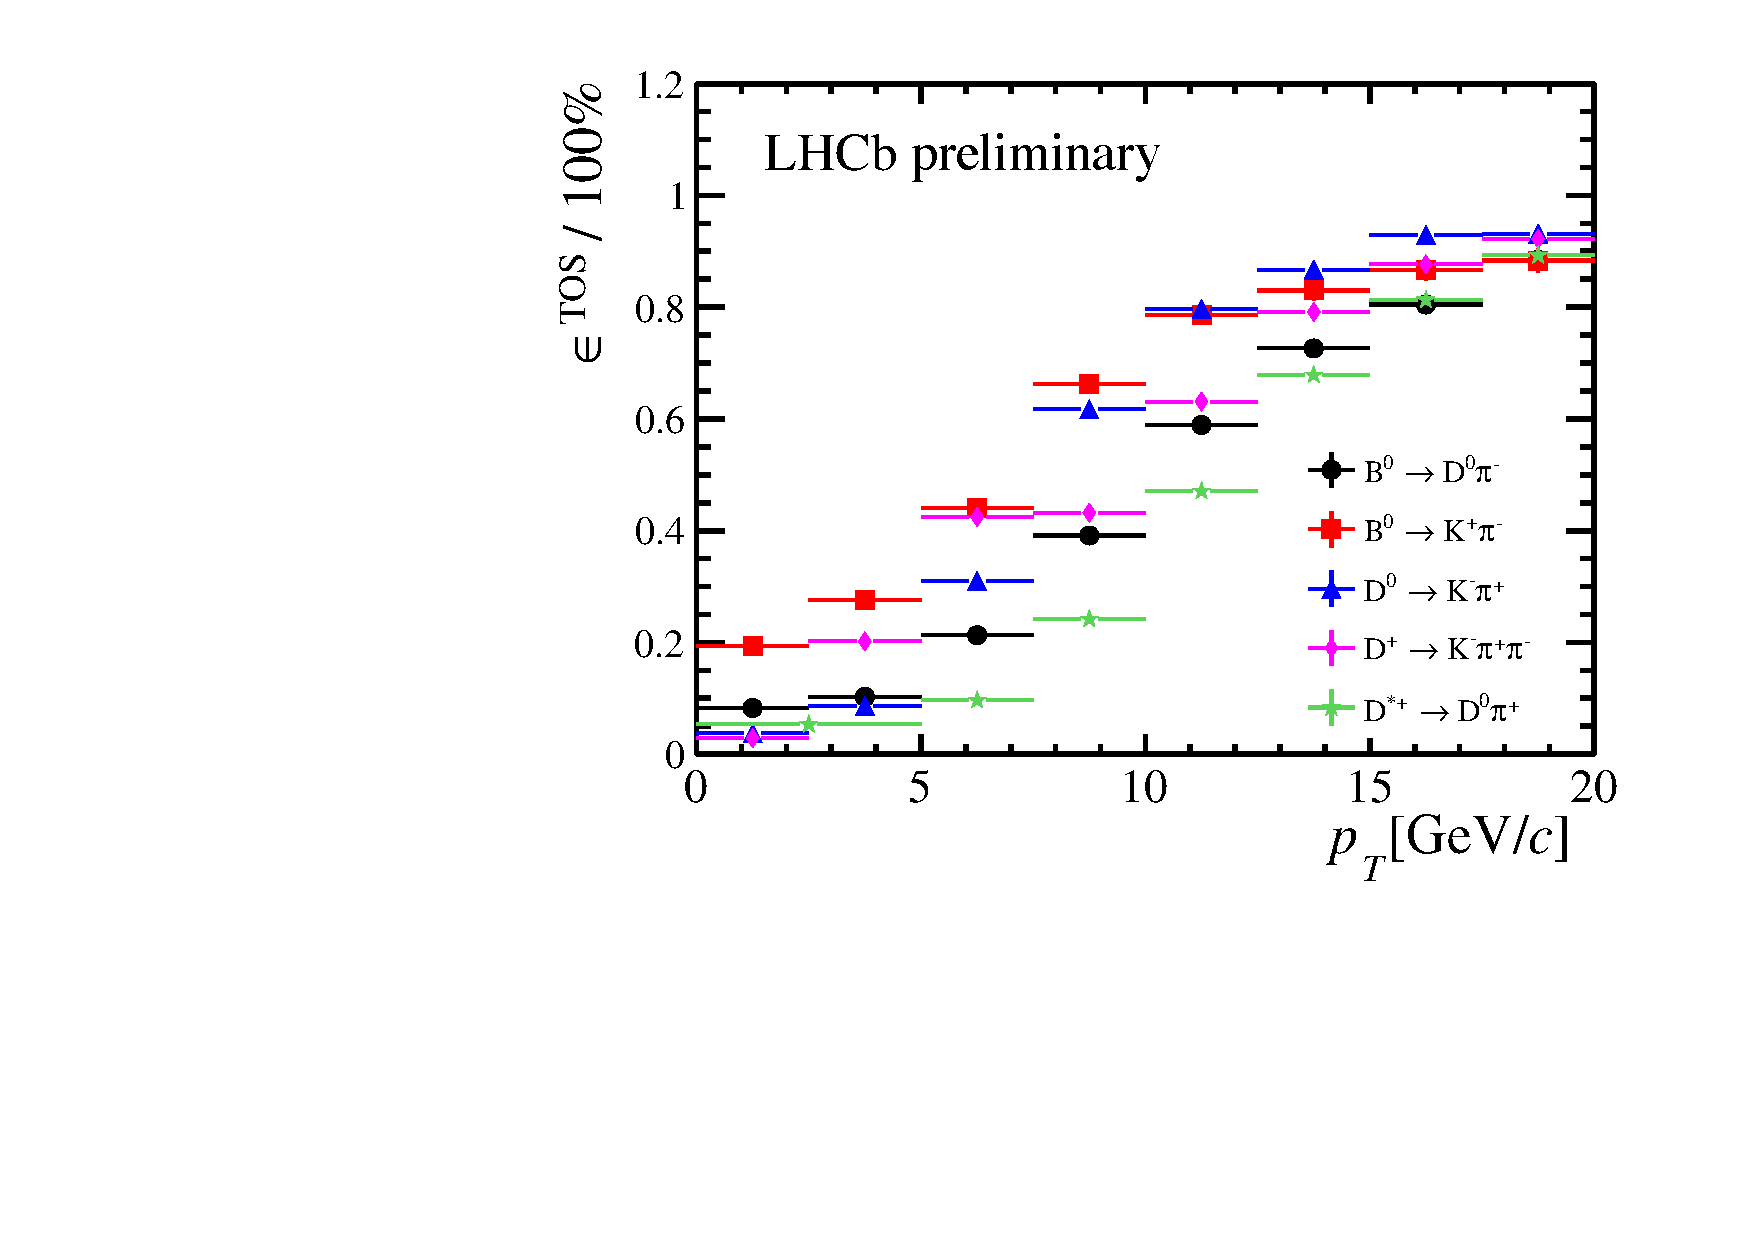
\includegraphics[width = 0.5\textwidth]{figs/detector/Fig21_L0Hadron_PT.pdf}\put(-50,90){(b)}%
	%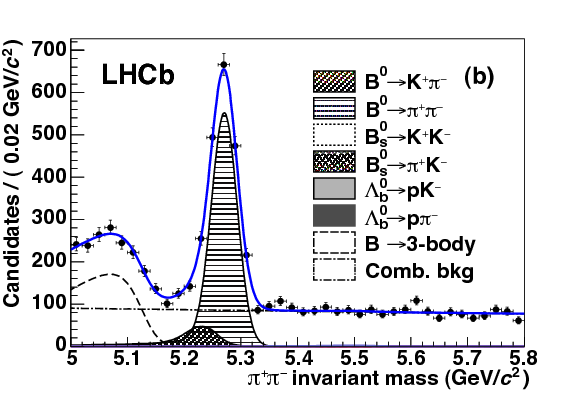
\includegraphics[width = 0.5\textwidth]{figs/detector/b2hhpid.png}%
	\caption{ (a) \Gls{TOS} efficiency as a function of $p_{T}$ for muon-based decisions. (b) \Gls{TOS} efficiency for different decays using L0 hadron trigger lines. Figures from \cite{Albrecht:2013fba}. }  
	\label{fig:L0Perf}
\end{figure}


 The software-based \Gls{HLT} then further reduces the rate from 1 \mhz down to $5$ \khz which can be recorded to long-term storage. The first stage of the \Gls{HLT}, (\Gls{HLT1}), performs limited track reconstruction and hence makes a decision based on the presence of charged particles in the event. \Gls{HLT1} uses \Gls{VELO} hits to reconstruct \Gls{PV}s and \Gls{VELO} tracks by using 3D pattern recognition. As \Gls{LHCb}'s primary mission is to study decays of hadrons containing $b$ and $c$ quark, \Gls{HLT1} will make \DIFaddbegin \DIFadd{a }\DIFaddend decision based on the track being displaced (having \DIFaddbegin \DIFadd{a }\DIFaddend high \Gls{IP}) with respect to the \Gls{PV}. For events selected by the \texttt{L0Muon}, an attempt is made to match the \Gls{VELO} tracks to hits observed in the vertical plane in the muon chambers, where the magnetic field of the dipole will not make them bend. By computing the track $\chi^2$, the potential muon track candidates are selected. Finally, the \Gls{VELO} tracks and muon tracks are extrapolated into the \Gls{OT} or \Gls{IT} trackers, allowing for so called \textit{forward tracking}, whereby $p$ and $p_{T}$ requirements are imposed to reduce processing time. Each track is then fitted with  a fast Kalman filter providing the $\chi^2$ of the fit. The corresponding performance of \DIFaddbegin \DIFadd{the }\DIFaddend \Gls{HLT1} trigger lines are shown in~\autoref{fig:Hlt1Perf}(a)(b).


\begin{figure}[!h]
	\centering
	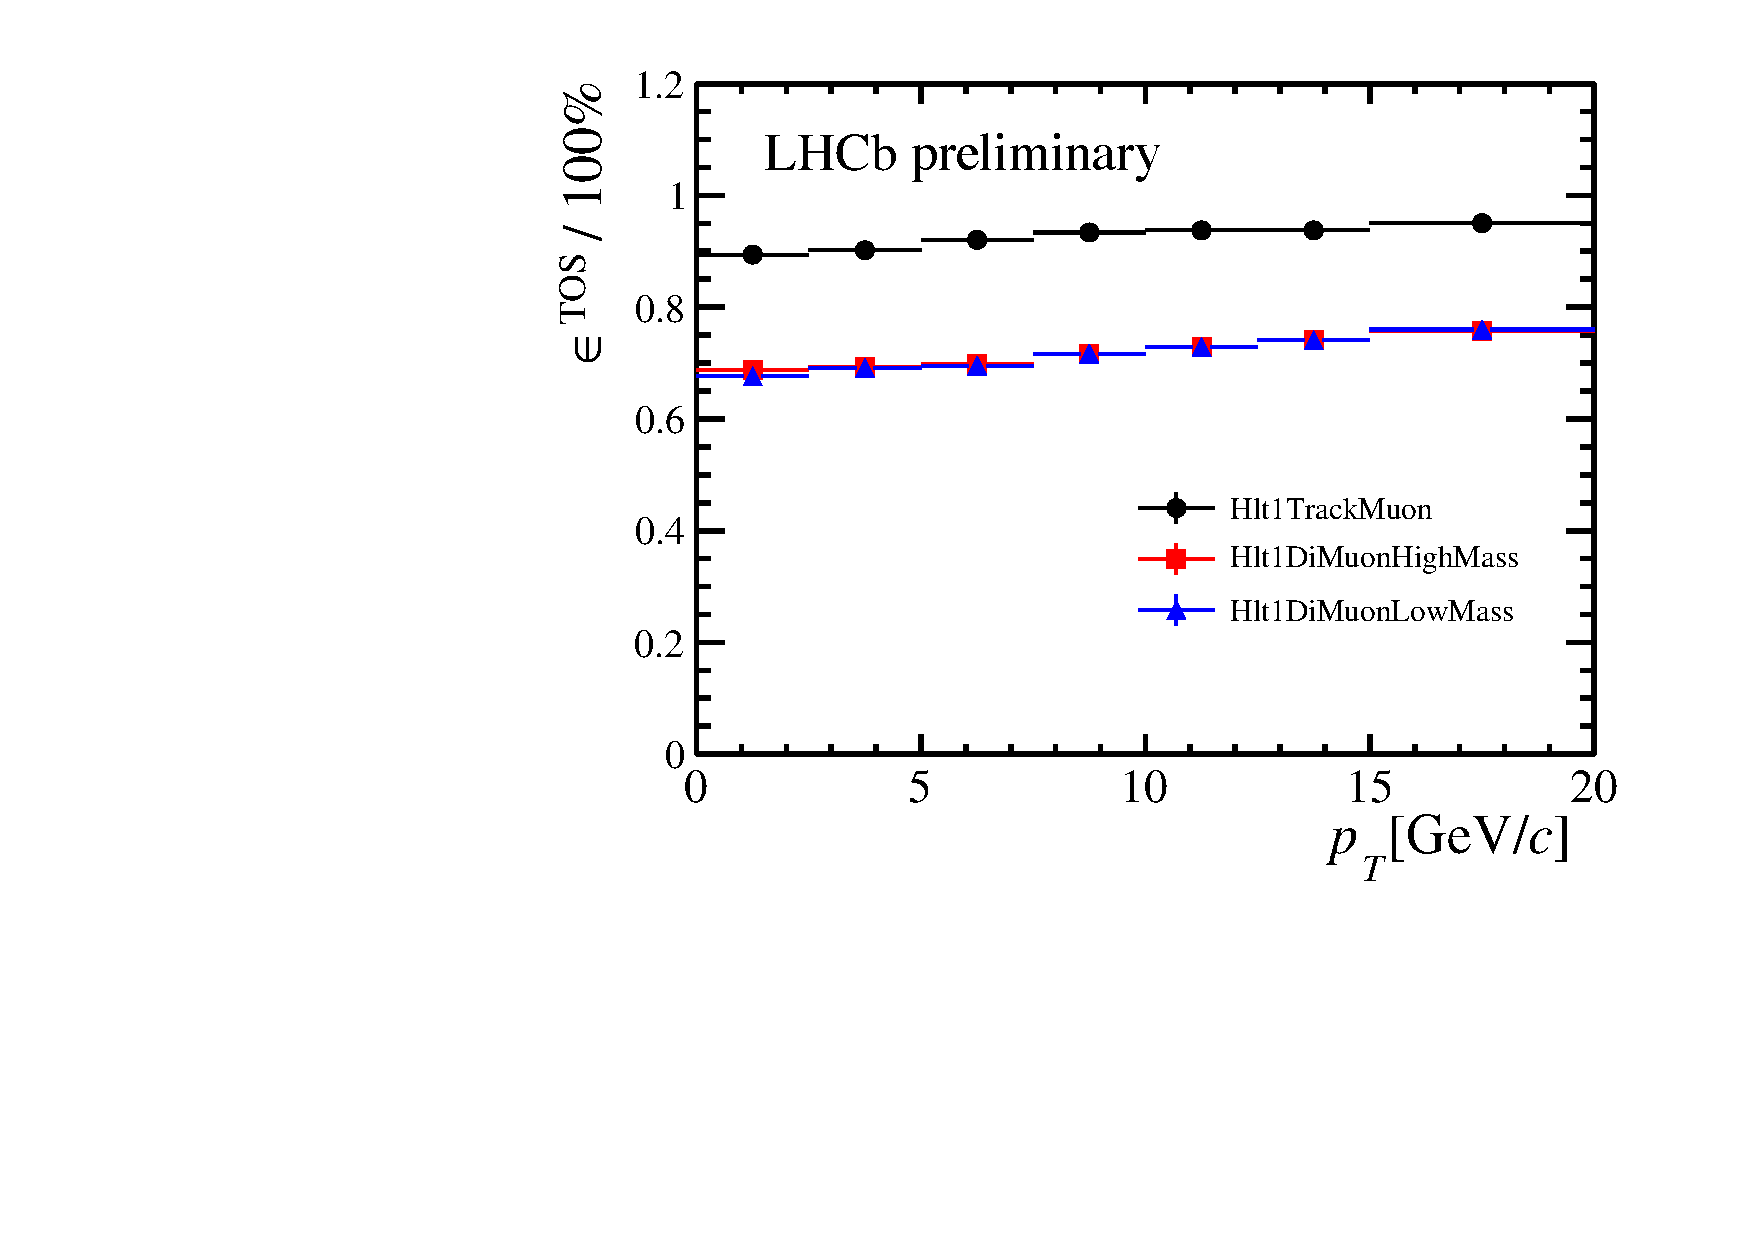
\includegraphics[width = 0.5\textwidth]{figs/detector/Fig3_Hlt1MuonEff_PT.pdf}\put(-50,140){(a)}%
	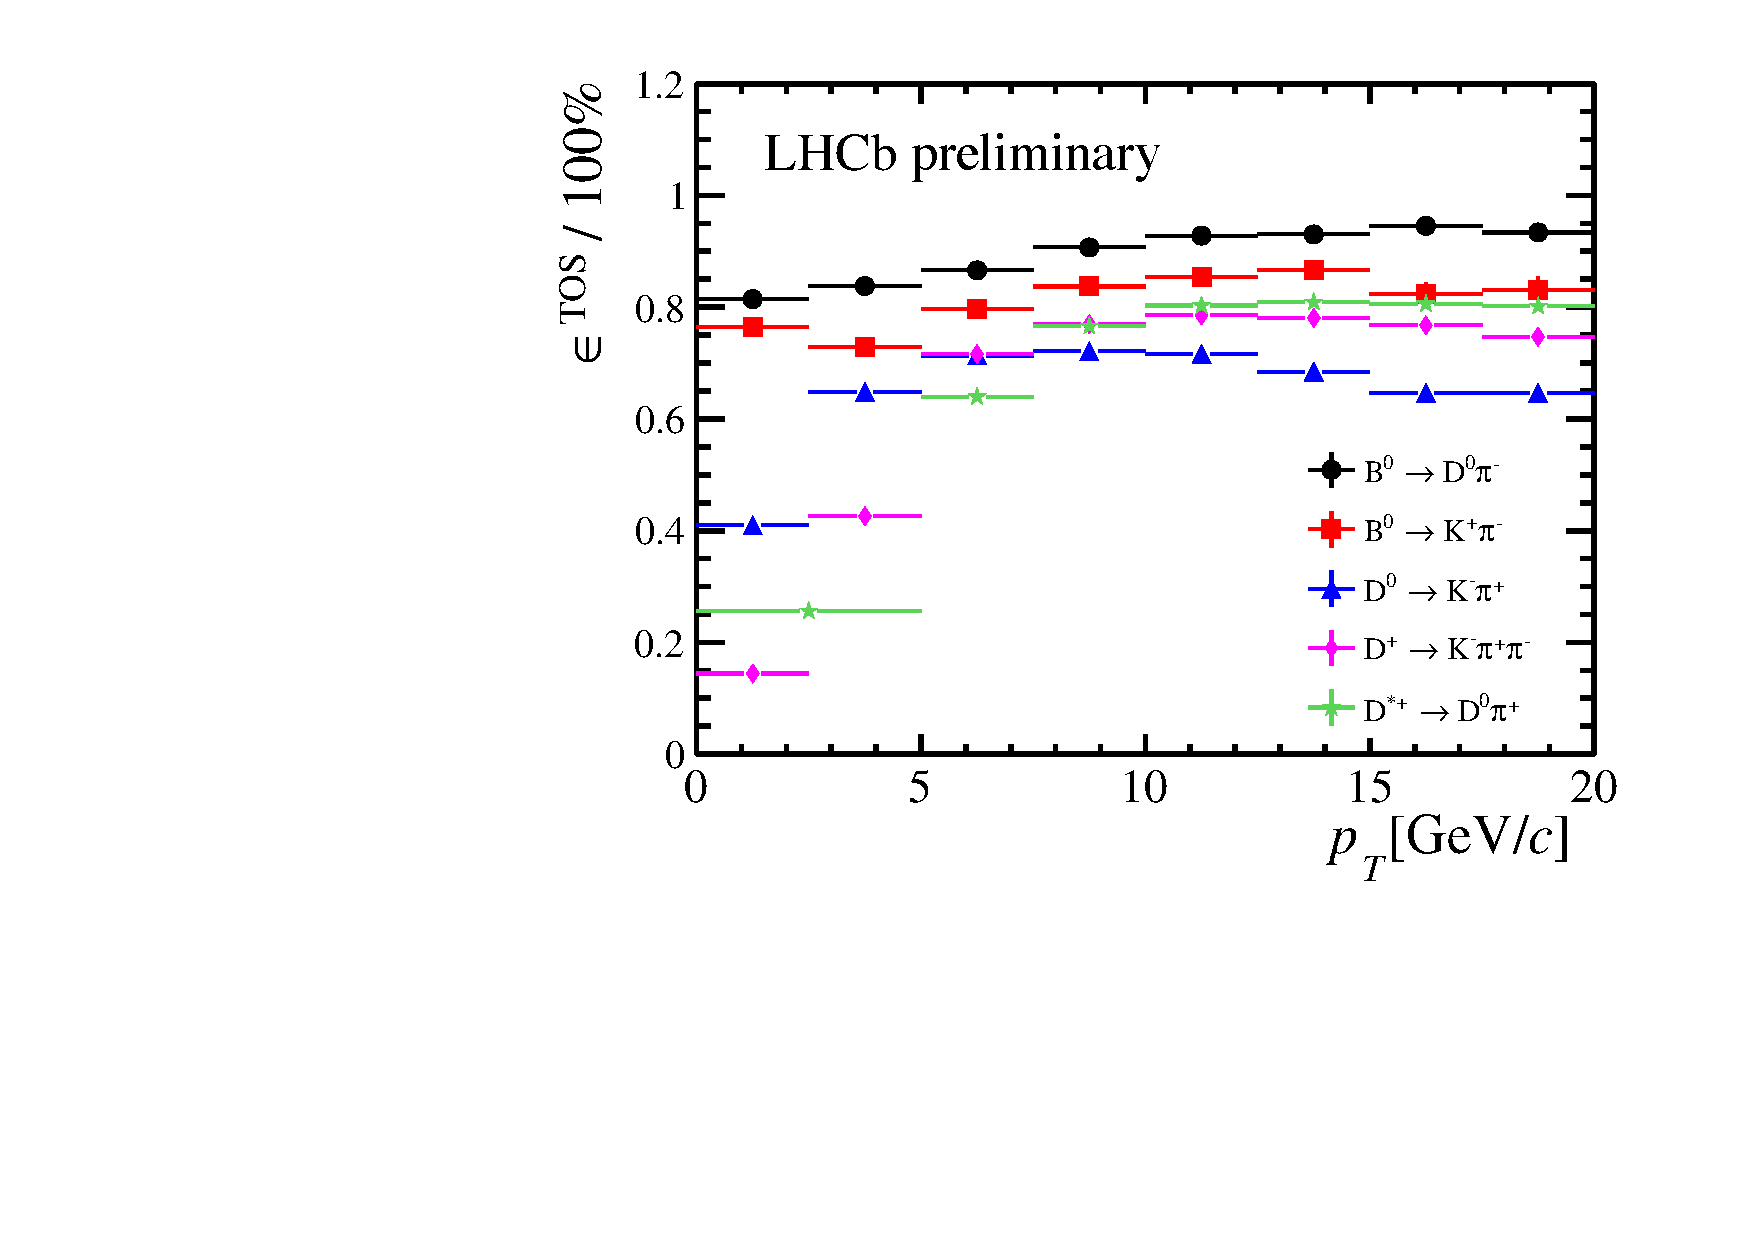
\includegraphics[width = 0.5\textwidth]{figs/detector/Fig5_Hlt1TrackAllL0_PT.pdf}\put(-50,140){(b)}%
	%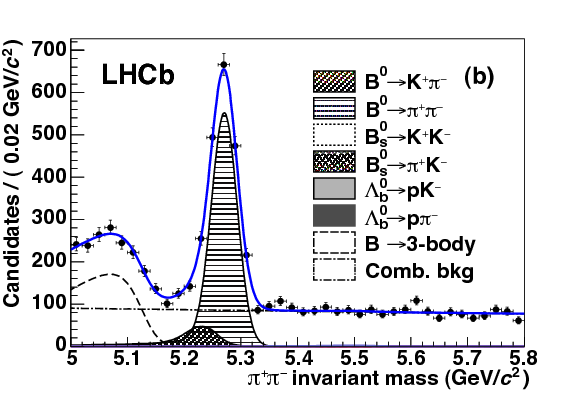
\includegraphics[width = 0.5\textwidth]{figs/detector/b2hhpid.png}%
	\caption{ \Gls{HLT1} efficiencies of the corresponding triggers using the same proxy as in~\autoref{fig:L0Perf}. Figures from \cite{Albrecht:2013fba}. }  
	\label{fig:Hlt1Perf}
\end{figure}

The second stage \Gls{HLT2} reduces the rate to 5 \khz that can be safely written to disk. \Gls{HLT2} consists of a series of decisions based on a full reconstruction of either groups of decays or specific decay modes. \textit{Topological triggers} exploit the vertex and track information (topology) of $b$-hadron decays. By employing multivariate techniques 2-,3- or 4-body decays that are well separated from the \Gls{PV} are reconstructed. To account for decays where a final state particle is not fully reconstructed, the corrected mass (will be defined in~\autoref{eq:corrm}) serves as an input variable in the the \Gls{BDT}. Dedicated lines are also written to reconstruct muon and dimuon channels allowing for both prompt $J/\psi$ and $B\rightarrow J/\psi X$ studies. Finally there are \textit{Exclusive triggers} concentrating on selecting events with $D$ mesons. They perform \DIFaddbegin \DIFadd{a }\DIFaddend selection which is very similar to the offline selection but without \Gls{PID} cuts.% and with \textit{prescales} required, where only a certain fraction of events is allowed to pass through.



Between the Run \Rn{1} and Run \Rn{2} period there has been a change in how the software trigger operates, which can be seen in~\autoref{fig:TriggerChange}. As more computing resources were introduced for both \Gls{HLT1} and \Gls{HLT2}, \Gls{LHCb} took advantage in upgrading the trigger system by introducing an update of \DIFaddbegin \DIFadd{the }\DIFaddend calibration and alignment constants of the relevant subdetectors before the data is sent to permanent disk. \textit{Online reconstruction}, defined as being produced at the trigger farm, became the same as the \textit{offline reconstruction}, defined as reconstruction made when data reached the permanent disk. Hence, there is \DIFdelbegin \DIFdel{enhancement of }\DIFdelend \DIFaddbegin \DIFadd{an enhancement of the }\DIFaddend available information, such as the \Gls{PID} in the \Gls{HLT}, which can then be used at the trigger level. 


\begin{figure}[!h]
	\centering
	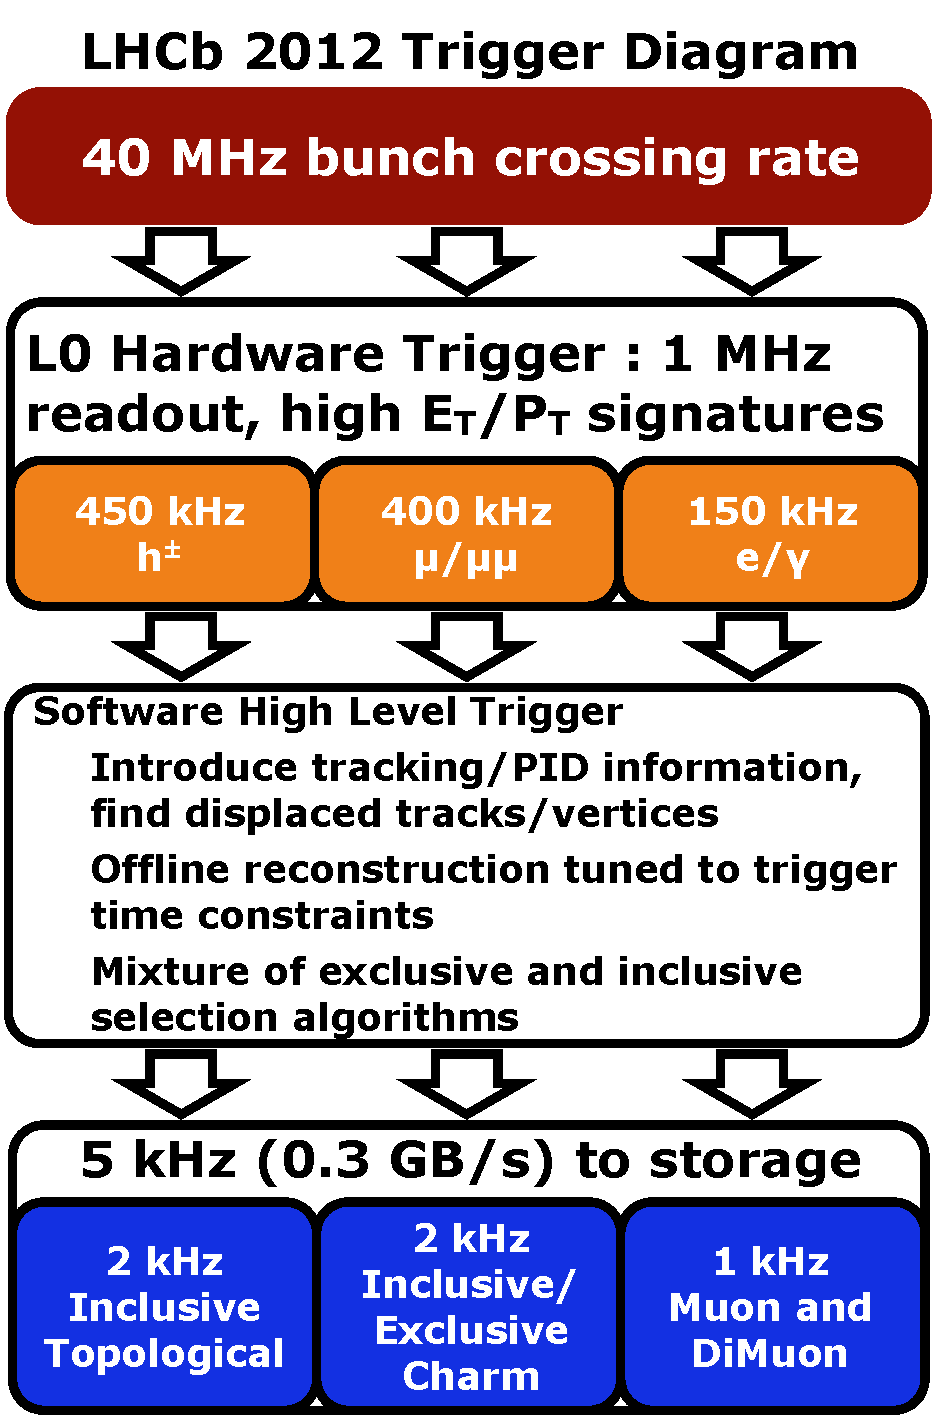
\includegraphics[width = 0.5\textwidth]{figs/detector/LHCb_Trigger_RunIAlg.pdf}%
	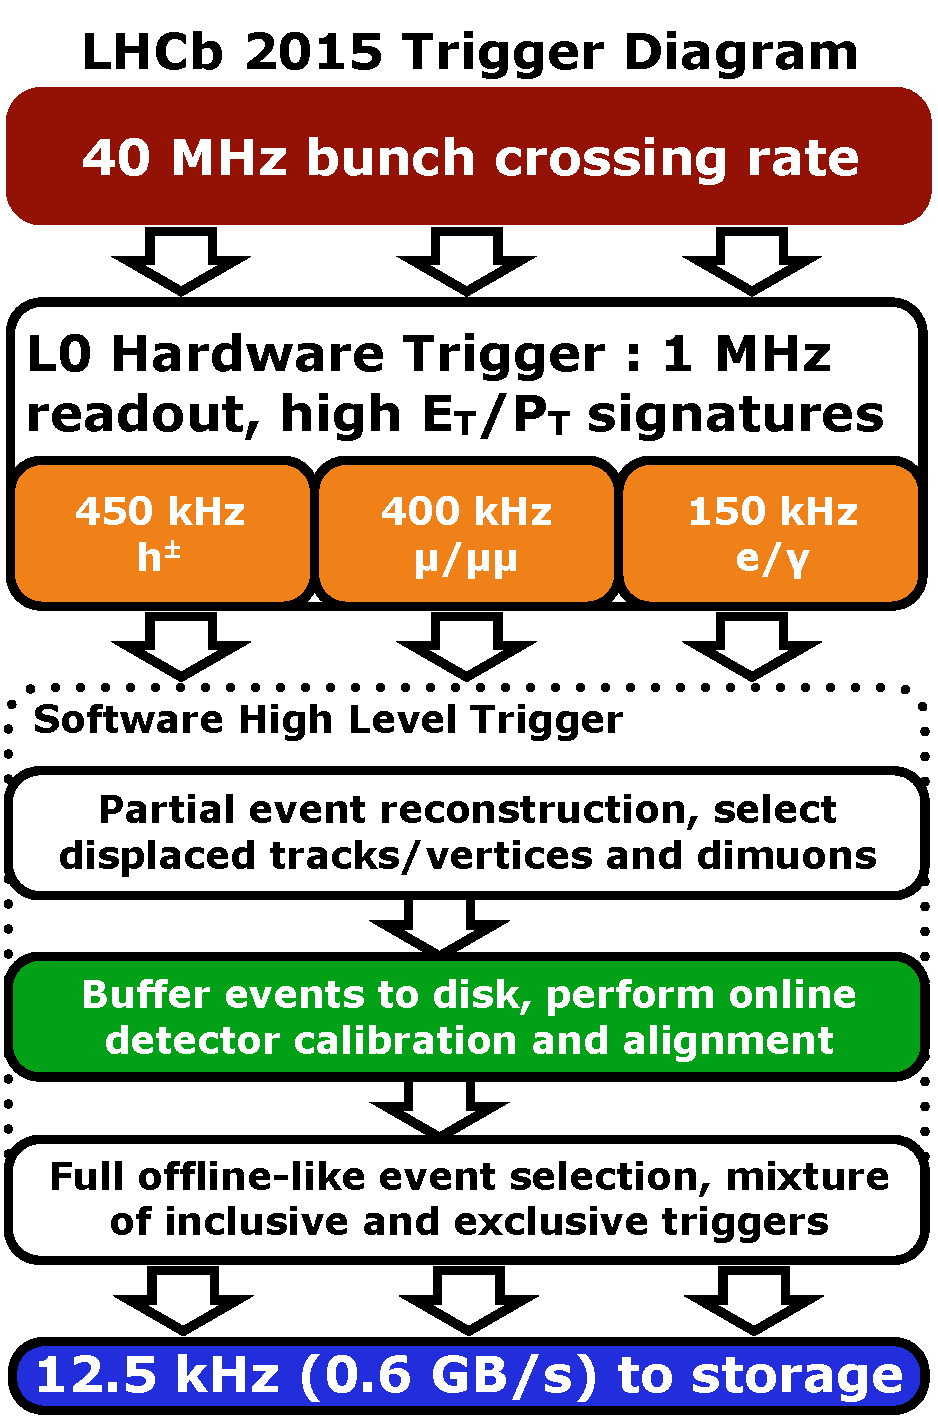
\includegraphics[width = 0.5\textwidth]{figs/detector/LHCb_Trigger_RunII.pdf}%
	%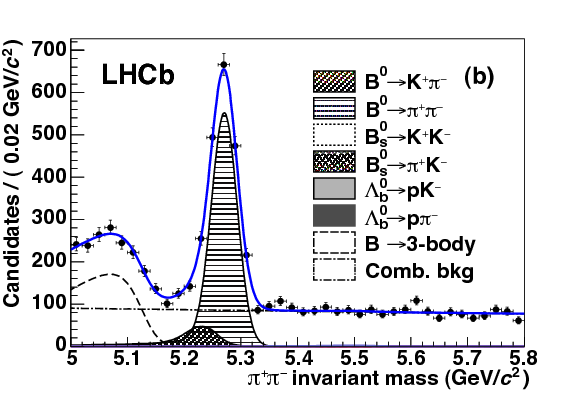
\includegraphics[width = 0.5\textwidth]{figs/detector/b2hhpid.png}%
	\caption{Trigger scheme differences between Run \Rn{1} and Run \Rn{2}. Figures from \cite{triggerscheme}.}  
	\label{fig:TriggerChange}
\end{figure}


\section{Simulation }
\label{simulationchap}
In order to optimise the event selections, determine efficiencies and model the backgrounds, a full Monte Carlo Simulation \Gls{MC} can be produced starting from simulation of the $pp$ collision to detector readout of the decay of interest produced. 
The $pp$ collisions within the \Gls{LHCb} configuration \cite{Belyaev:2011zza} are simulated with Pythia 6.4 \cite{pythia6} and Pythia 8.1 \cite{pythia8}. \Gls{LHCb} specific settings are mostly related to running conditions: luminosity, number of collisions per bunch crossing as well as contamination from other bunches, \textit{spill-over}. 

In the $pp$ collision, the $b$ and $c$ production mechanisms are simulated and then the following $b\bar{b}$ or $c\bar{c}$ pair is hadronized into hadrons of interest. In this thesis and the analysis presented, the \Bp meson is the hadron of interest. Hadrons are then further decayed using EVTGEN \cite{Lange:2001uf} into the chosen decay products. At this stage, different physics models or inputs from theory can be configured. % At the same time some initial CPU-friendly selection is established, usually requiring the hadrons to be contained within the forward detector's acceptance.
In order to account for the effects of \Gls{QED} radiative corrections, the PHOTOS \cite{photos} algorithm can be used. All of this combined establishes \textit{the generator-level simulation} of LHCb.


In the next phase, \textit{detector simulation}, the interactions of \DIFdelbegin \DIFdel{the }\DIFdelend all the particles with the detector, transport, as well as detector's response are simulated using the C++ GEANT4 toolkit \cite{Geant4},\cite{Agostinelli:2002hh}. \Gls{LHCb}'s interface to GEANT4 is detailed in Ref\cite{Clemencic:2011zza}. 

\subsection{Differences in Simulation and Data}
\label{detpid}
Despite the complexity and best intention of the \Gls{LHCb} simulation, there are several shortcomings that require corrections.
The most affected variables necessary for physics analyses that one needs to consider are \Gls{IP} resolution, track reconstruction efficiencies, \Gls{PID} variables and track occupancy.

The \Gls{IP} resolution shows a better trend in the simulation then in the data due to the mismodelling of the material description \DIFdelbegin \DIFdel{of }\DIFdelend \DIFaddbegin \DIFadd{in }\DIFaddend the \Gls{VELO} simulation. As shown in~\autoref{fig:IPRES}(a)(b)  the \Gls{IP} resolution does greatly differ depending \DIFaddbegin \DIFadd{on }\DIFaddend the variation of material density of \Gls{VELO}. Around $\phi=\pm\pi/2$, where the two \Gls{VELO} parts overlap, the material difference causes the discrepancy. It can be corrected either by reweighting to data or by smearing the resolution with a Gaussian distribution.

\begin{figure}[!h]
	\centering
	\includegraphics[width = 0.5\textwidth]{figs/detector/IPXRes-Vs-InversePT-Compare2012DataToMC.pdf}\put(-50,60){(a)}%
	\includegraphics[width = 0.5\textwidth]{figs/detector/IPXRes-Vs-Phi-Compare2011DataToMC.pdf}\put(-50,60){(b)}%
	\caption{ (a) \Gls{IP} resolution in \DIFaddbeginFL \DIFaddFL{the }\DIFaddendFL x-direction comparing the data and simulation \DIFdelbeginFL \DIFdelFL{output }\DIFdelendFL for \DIFaddbeginFL \DIFaddFL{the }\DIFaddendFL 2012 data-taking period. (b) \Gls{IP} resolution in \DIFaddbeginFL \DIFaddFL{the }\DIFaddendFL x-direction comparing the data and simulation \DIFdelbeginFL \DIFdelFL{output }\DIFdelendFL for \DIFaddbeginFL \DIFaddFL{the }\DIFaddendFL 2011 data-taking period as a function of angle, $\phi$. Figures from \cite{LHCbVELOGroup:2014uea}. }  
	\label{fig:IPRES}
\end{figure}


Track reconstruction efficiency is also not reproduced very well in certain \DIFdelbegin \DIFdel{kinematical }\DIFdelend \DIFaddbegin \DIFadd{kinematic }\DIFaddend bins, again due to modelling of scattering interactions.

The most critical problem that needs to be addressed in the presented analysis \DIFdelbegin \DIFdel{are }\DIFdelend \DIFaddbegin \DIFadd{is }\DIFaddend the inaccuracies of the \Gls{PID} variables, which are mismodelled in the simulation. \DIFdelbegin \DIFdel{The origin of this }\DIFdelend \DIFaddbegin \DIFadd{This }\DIFaddend problem arises as a consequence of \DIFaddbegin \DIFadd{the }\DIFaddend much lower estimate of low momentum tracks in the detector\DIFaddbegin \DIFadd{, }\DIFaddend making the photoelectron background underestimated. This results in better \DIFdelbegin \DIFdel{performance of separation power }\DIFdelend \DIFaddbegin \DIFadd{separation }\DIFaddend in simulation and is corrected using \DIFaddbegin \DIFadd{a }\DIFaddend data calibration. 

Therefore the \gls{PID} efficiency is usually obtained from \DIFaddbegin \DIFadd{the }\DIFaddend data. More specifically, this is done by using high-yield and relatively background-free calibration channels, where the species of the particle can be deduced from kinematics of the decay. \DIFdelbegin \DIFdel{Standard }\DIFdelend \DIFaddbegin \DIFadd{A standard }\DIFaddend set of these channels are "housed" in a \texttt{PIDCalib} package \cite{Anderlini:2202412}. \DIFdelbegin \DIFdel{In }\DIFdelend \DIFaddbegin \DIFadd{With }\DIFaddend this package, \DIFaddbegin \DIFadd{the }\DIFaddend \gls{PID} efficiency can be computed in a given kinematic region of interest. 



%%%\thesubsection{Boosted Decision Trees}
\label{app:bdt}
%% As the HLT trigger makes use of a machine learning technique called a Boosted Decision Trees (BDT), an aside will be taken here to introduce the concept.

Many rare decay analyses make extensive use of BDTs and they are important in the \Lbpi analysis. Firstly, the concept of a decision tree is introduced followed by a brief explanation of boosted decision trees.

A decision tree, in the context of data mining, is a supervised machine learning method which allows for the prediction of the value of a target variable based on several input variables. In particle physics, the purpose of the decision tree is to classify an event as being either signal or background, based on the event's input variables. The input variables, $\left\{x_{i}\right\}$, are various physics parameters. % and in the case of the HLT include the minimum $P_{T}$  and mass of the particle.
% and $IP_{\chi2}$ (where the $IP_{\chi2}$ is the difference in the $\chi2$ of the fit to the PV when the track whose $IP_{\chi2}$ is being measured is added and then removed)
Each cut point in the tree is referred to as a node and the final nodes are referred to as leaves. A very simple example is shown in~\autoref{fig:BDT}. The purity, $P$, of a leaf refers to the fraction of the weight of a leaf due to signal events, e.g. if a leaf had 20 signal events and 15 background events it would have a purity of 0.75. If a leaf has a purity larger than 0.5 it is deemed to correspond to signal and if lower, to background.
\begin{figure}
  \centering
  \includegraphics[scale = 0.7]{figs/BDT.png}
  \caption{An example decision tree. The S and B stand for `Signal-like' and `Background-like'. The $\beta_{i}$ variables refer to the cut values chosen by the machine learning algorithm after the tree has been trained on signal and background samples. The blue ovals represent final nodes called leafs, which each leaf having an associated purity, i.e. the fraction of the weight of a leaf due to signal events.}
  \label{fig:BDT}
\end{figure}

A decision tree is constructed by a process called training. For this, samples of known signal and background events are used. These samples could be either simulation or data. For each $x_{i}$ the best dividing point is decided, that is, the cut that gives the best separation between signal and background. This optimum point is decided by using the Gini index defined as

\begin{equation}
Gini  = \sum^{n}_{i = 1} W_{i} P(1 - P),
\end{equation}
where $W_{i}$ is weight of the $i^{th}$ event, which would generally be unity for the case of a non-boosted decision tree. 
The cutting point is then found by maximising the separation, $\Delta$, between the Gini index of the parent node and the combined Gini index of the child nodes, as given in~\autoref{eq:diffgini} 
\begin{equation}
 \Delta =   Gini_{parent} - Gini_{child_{1}} - Gini_{child_{2}}.
  \label{eq:diffgini}
\end{equation}
The depth of a tree (the maximum number of cuts or nodes) is normally a number specified before the training begins.
%\cite{miniboone}

Boosting a decision tree involves training many trees ($\mathcal{O} \sim 1000$) and giving misclassified events a higher weight. A misclassified event is defined as a known signal event being placed on a background leaf and vice versa. By giving the events which are difficult to classify more weight, the next tree to be trained will effectively have to work harder in order to classify events correctly. %The way in which events are weighted (or boosted) can vary, and in the 

The total score on an event is deduced by following an event through from tree to tree and, for the algorithms used in this thesis, is simply given by the weighted sum of the scores over the individual trees.

%% This weighting is done using the total number of misclassified events in a tree. The error of the $m^{th}$ tree is defined as
%% \begin{equation}
%%   err_{m}=\sum_{j}W_{j}; j = \text{misclassified event}.
%% \end{equation}
%% The weight (or score) of this tree is then given as
%% \begin{equation}
%%   \alpha_{m} = C \ln\frac{1-err_{m}}{err_{m}},
%% \end{equation}
%% where $C$ is  a constant. The increase in weight of a misclassified event is given as
%% \begin{equation}
%%   W_{i} = W_{i} e^{\alpha_{m}}.
%% \end{equation}
%% All weights are then renormalized, $W_{i} \to W_{i}/\sum^{N}_{i = 1} W_{i} $, and the total output, $T(x_{i})$, for an event $i$ is given as
%% \begin{equation}
%%   T(x_{i}) = \sum^{N_{tree}}_{m = 1} \alpha_{m}T_{m}(x_{i}).
%% \end{equation}

Data sets are split into two (or more) sub samples, where one half is used for training the tree and the other is used for testing the tree, and the distributions of the event scores (the BDT output) for training and testing samples are compared for signal and background. Cases where the training sample performs better than the testing sample are referred to as over-trained trees, which is often due to the BDT becoming sensitive to the statistical fluctuations of the training sample.%Most BDT's used within LHCb produce a BDT output ranging from -1 to 1, with more positive outputs being associated with a more signal-like data candidate.

 The distribution of events scores for a given dataset can then be cut on in order to increase the fraction of signal events.

%Alternatively, the over performance of the training sample could be due to there being correlations between the  signal and background proxies used for training which do not exist in the actual data. 
%% The value for $G$ is calcualted using the Gini index which is a function of the purity $p$.


%% The creates two new nodes and the algorithum is applied again to these nodes. Adapative boosting is when misclassfied events (i.e. in the case when you have a signal training sample the event is classified as abckground and vice versa) and given higher weighs 
%% For each xi the splitting value that gives the best separation of the events into two child nodes -- one with mostly signal events, the other with mostly background events -- is found. The variable and split value giving the best separation are selected and two new nodes are created, one corresponding to events satisfying the split criterion (labeled P for passed in the above figure), the other containing events that failed it (labeled F). The algorithm is then applied recursively to the two child nodes. This process contains untill the specified maximum number of given nodes. When the splitting stops, the terminal node is called a leaf, with an associated purity, the weighted signal fraction of the training sample in this node

%The primary vertex is defined as being within a raduis of 300\mum of the mean position of the $pp$ interation. 



\chapter{Handling of Trimuon Correlations at LHCb}
\label{chap:trimuon}


\textit{This chapter discuss issues associated with three muons passing through the detector. Two collimated muons may traverse through the same parts of the detector if they have the same charge, causing problems in resolving their individual tracks. Therefore, ghosts and clones are much more likely to occur. In LHCb, a plethora of muon \Gls{PID} variables are used to suppress these types of spurious tracks. However, the usage of \gls{PID} variables in an analysis in \gls{LHCb} brings its own challenges. As the simulation is not able to estimate \gls{PID} efficiencies correctly, most of the \gls{PID} efficiencies are taken from control samples. New control samples for \Bmumumu are considered as the \Gls{PID} efficiencies depend strongly on the number of muons in the detector and in the standard misID control samples there is just a single muon in each event.}

\color{black}

\section{Muon PID Variables}
\label{otherpid}
In addition to the muon identification variables mentioned in~\autoref{muonID}, there is a further set of criteria for selecting muons. In this section a summary of the variables used in the \DIFdelbegin \DIFdel{analysis of the }\DIFdelend \Bmumumu \DIFaddbegin \DIFadd{analysis }\DIFaddend is discussed.

\subsection{Binary Muon PID Variables }
Similar to \texttt{isMuon} shown in~\autoref{tab:ismuontab}, there are more binary variables, such as \texttt{isMuonTight}, that can help with \DIFaddbegin \DIFadd{the }\DIFaddend classification of muons. As its name suggests, \texttt{isMuonTight} has stronger conditions to satisfy as compared to \texttt{isMuon}. 

In each muon station (\gls{muonstation}) a field of interest, \gls{FOI} is defined as %a function of momentum $p$ in a following way:
\begin{equation}
	FOI_{x,y}=\rho^{0}_{x,y}+\rho^{1}_{x,y}\cdot \exp \left(\frac{\rho^{2}_{x,y}\cdot p}{\gevc} \right),
\end{equation}
where $x,y$ are the dimensions perpendicular to the direction of the beam, $p$ is \DIFaddbegin \DIFadd{the }\DIFaddend momentum of the muon, $\rho^{i}_{x,y}$ are three \DIFdelbegin \DIFdel{dimension-dependent }\DIFdelend \DIFaddbegin \DIFadd{dimensional }\DIFaddend parameters tuned to give the best performance, by maximizing efficiency \DIFdelbegin \DIFdel{to }\DIFdelend \DIFaddbegin \DIFadd{versus }\DIFaddend misID rate. \DIFaddbegin \DIFadd{This }\gls{FOI} \DIFadd{can be thought of as cone whose radius depends on the $p$.
}\DIFaddend 

When a muon passes through the detector, it leaves hits ($h_{x,y}$ coordinate) in a pad with size $pad_{x,y}$ of each muon station. From the tracks formed in the tracking part of the detector, coordinates $E_{x,y}$ are obtained by \DIFdelbegin \DIFdel{extrapolating }\DIFdelend \DIFaddbegin \DIFadd{extrapolated }\DIFaddend the tracks into the muon stations. The hits are considered to be within the \gls{FOI} if they satisfy the condition that $|| h_{d} - E_{d} || < FOI_{d} \cdot pad_{d}$ for both d={x,y}. 

\color{black}

The detector information is read out in the $x$ and $y$ direction separately. The pad slicing according to this read-out scheme is known as \textit{physical} slicing of pads. However, as seen in~\autoref{fig:pads}, the overlapping $x$ and $y$ \textit{physical} pads can be grouped into \textit{logical} pads, which give information about $x$ and $y$ simultaneously. This leads to two groups of hits according to pad type: uncrossed hits - registered within \textit{physical} pads only, and crossed hits - given by \textit{logical} pads. Whereas \texttt{isMuon} only requires \DIFaddbegin \DIFadd{a }\DIFaddend positive decision from uncrossed hits, \texttt{isMuonTight} requires \DIFaddbegin \DIFadd{a }\DIFaddend positive decision based on crossed hits. 


\begin{figure}[!h]
        \centering
        %\includegraphics[width = 0.3\textwidth]{figs/trimuon/poze.jpg}
        \includegraphics[width = 1.0\textwidth]{figs/trimuon/fig2.pdf}
        \caption{Schematic view of the muon station slicing into x-y pads. This is the left quadrant of the M1 station, showing decreasing granularity of the muon stations away from the beam pipe. This figure has been taken from \cite{LHCb-DP-2012-002}. M1R1 is the innermost region and M1R4 is the outermost region of the M1 station. }
        \label{fig:pads}
\end{figure}



\DIFaddbegin \begin{figure}[!h]
        \centering
        %DIF > \includegraphics[width = 0.3\textwidth]{figs/trimuon/poze.jpg}
        \includegraphics[width = 0.5\textwidth]{figs/trimuon/crossedhits.pdf}
	\caption{\DIFaddFL{Difference between crossed and uncrossed hits. A hit
in a muon station is considered a crossed hit if it is registered both by a
horizontal and a corresponding vertical strip. If a hit is only seen by either,
	it is considered uncrossed. This figure has been taken from \mbox{%DIFAUXCMD
\cite{Dungs:2015mml}}%DIFAUXCMD
.}}
        \label{fig:pads}
\end{figure}


\DIFaddend \subsection{Muon PID Variables Based on Sharing Hits }
\label{bugs}

Another way of identifying muon tracks is based on the variable, \texttt{nShared}, which identifies the number of tracks with shared hits in the muon stations. For each hit within the \gls{FOI} of an extrapolated track, the \texttt{nShared} algorithm will check whether any other track was built using the given hit. In this case, the \texttt{nShared} variable of the muon track which has the bigger distance between the extrapolation coordinates and the hit coordinates is increased by 1. Hence this integer \gls{PID} variable helps suppressing \textit{ghost} tracks and \textit{clones} if no tracks have hits in common with the owner of the track (\texttt{nShared=0}).

%\subsection{Different \texttt{nShared} definitions for Run \Rn{1} and Run \Rn{2}
%To make sure that muons for \Bmumumu are not coming from these spurious tracks,  \texttt{nShared==0} for all three muons is required. These three muon tracks will not to share hits in muon stations with any other downstream or long tracks. In analysing data, there were features in the Muon ID alghorithm, software that calculates most of muon \gls{PID} variables, which changed between Run \Rn{1} and Run \Rn{2} and will be discussed in greater detail, as it impacts the selection performed for \Bmumumu search.
The muon identification software algorithms evolved significantly between the processing of Run \Rn{1} and Run \Rn{2} data. This included bug fixes, improvements and the introduction of new bugs. In the \Bmumumu analysis, this has to be taken into account.


The first feature that is different between Run \Rn{1} and Run \Rn{2} arises from the calculation of the distance between the extrapolation and the hit in \DIFaddbegin \DIFadd{the }\DIFaddend \texttt{nShared} algorithm.
In \textit{Stripping 21} (where \textit{stripping} is a preselection) used for 2012 and \textit{21r1} used for 2011 data, it was discovered that the distance between an extrapolated track and a hit was wrongly calculated. This mistake was corrected before \textit{Stripping 23}, used for analysing 2015 data. 

Secondly, information from the M1 station was used to calculate distances, even though M1 information is not usually used for the Muon ID algorithms.  For analysts, this feature was present across all reconstruction software, meaning that simulation and data is affected in the same way.

In \textit{Stripping 23}, the Muon ID algorithm was rewritten to adapt to the parallelisation that needs to be done in order to meet the criteria for the upgrade of \gls{LHCb}. There were two mistakes introduced prior to 2015 data taking.
Firstly, an array was defined with 4-elements $[0,3]$ to store information about \DIFaddbegin \DIFadd{the }\DIFaddend $x$ and $y$ coordinates of the hits. However, an iteration occurred by filling elements 1 to 4 of the array (M2-M5\DIFdelbegin \DIFdel{station}\DIFdelend ) resulting in a 5-element array where the 0-th element was not filled. Despite this, it turns out to be well-behaved and has no impact on physics. \DIFaddbegin \DIFadd{There was no significant implication for any analysis arising from this mistake.
}\DIFaddend 

Further in the process, however, this information is used to calculate the sum and average of distances per station between the hits and extrapolations. This algorithm again iterates over $[0,3]$ arrays, meaning that no information is used from the M5 muon station. This obviously has an effect, but again it is consistent across the versions of the reconstruction software used for the processing of Run \Rn{2} data.

%\newline Summary of these features can be found in \href{https://indico.cern.ch/event/612764/contributions/2567244/attachments/1449649/2234804/20170426\_nShared.pdf}{\color{blue} in this presentation} 
The interplay between all these features for \bjpsimumuk decays \DIFdelbegin \DIFdel{, }\DIFdelend can be seen in~\autoref{fig:nSharedvar}, which sees a shift in distribution of \texttt{nShared} for 2016 data taking, making the muons less isolated.

\begin{figure}[h!]
\centering
\includegraphics[width=0.5\linewidth]{trimuon/plotvariablewantlogtruemu1_nSharedJPSIKMC.pdf}\put(-40,133){(a)}
\includegraphics[width=0.5\linewidth]{trimuon/plotvariablewantlogtruemu1_nSharedJPSIKDATA.pdf}\put(-40,133){(b)}
	\caption{(a) \texttt{nShared} variable distribution for the positive muon in \bjpsimumuk decays in (a) simulation and (b) data. Different stripping versions corresponding to 2012 (\textit{Stripping 21}), 2011 (\textit{Stripping 21r1}), 2016 (\textit{Stripping 26}) data-taking are shown. The distributions are normalised to have the same area. There is \DIFaddbeginFL \DIFaddFL{a }\DIFaddendFL shift of distribution in \textit{Stripping 26} towards less isolated tracks. The proportion of muon tracks that share no other hits with other tracks is smaller, whereas the proportion of the tracks sharing hits with other muon track is \DIFdelbeginFL \DIFdelFL{increasing}\DIFdelendFL \DIFaddbeginFL \DIFaddFL{increased}\DIFaddendFL .}
\label{fig:nSharedvar}
%\vspace*{-1.0cm}
\end{figure}

Using the same calibration channels as in~\autoref{muonperf}, misID and ID rates can be seen in~\autoref{fig:nSharedRun1andRun2}. As the tracks tend to be less isolated in \textit{Stripping 26} used for 2016 data, typical of non-signal like events, the misID rate is expected to be higher for the same working point (ID efficiency). While the issues highlighted here can be fixed with a reprocessing of the data, this is not expected to happen before 2019 or 2020.

\begin{figure}[h!]
\centering
%\includegraphics[width=0.52\linewidth]{compareRun1and2016selection/final_comparedirectly2012vs2015_nolog.pdf}%
\includegraphics[width=0.7\linewidth]{trimuon/final_pretty_2016_pion.pdf}
	\caption{ID and misID probabilities from standard calibration datasets from 2012 (\textit{Stripping 21}) and 2016 (\textit{Stripping 26}), binned using the default 2-dimensional binning scheme in momentum $p$ and pseudorapidity $\eta$. In this plot, ID and misID rates in the central bin of $\eta$, 2.375<$\eta$<3.25, and the first and second bin in $p$ are compared. This demonstrates that for the same pion ID efficiency, the misID rate is significantly higher in 2016 data.}
\label{fig:nSharedRun1andRun2}
%\vspace*{-1.0cm}
\end{figure}

\subsection{Muon PID Variables Based on Regression Techniques }
\label{muonPIDprobnn}
Similar to the DLLmu variable in~\autoref{muonID}, which combines all the information from the detector into a global likelihood, it is possible to feed all the different variables to a neural network, which can then produce an output corresponding to the probability of a particle to be of a certain species. \texttt{Probnn${x}$}, where $x$ is the species of interest, is calculated and can be used also for muon identification. Compared to $\rm{DLLx}$ variables, \texttt{Probnn${x}$} variables tend to have smaller correlation with the kinematics of the particle, and hence are more useful with decays where particles are soft, such as \Bmumumu. As with any machine learning algorithm, the selection of both the training sample and the input variables are important. In Run \Rn{1}, there were two tunings (trainings) introduced \texttt{V2} and \texttt{V3}, with more input variables in \texttt{V2}. Depending on the species of \DIFdelbegin \DIFdel{particles}\DIFdelend \DIFaddbegin \DIFadd{particle}\DIFaddend , \texttt{V2} or \texttt{V3} performed better. In the analysis of \Bmumumu, \texttt{Probnn${x}\_$V2} is used.


\section{Clones}
\label{cloniatkos}
When analysing decays with two muons of opposite charge, \DIFdelbegin \DIFdel{the }\DIFdelend \DIFaddbegin \DIFadd{one can rely on the fact that }\DIFaddend \gls{LHCb} magnet bends these two muons in two opposite directions. With two muons of the same sign, the muons will instead bend in the same direction and can stay close together in both the tracking system and the muon detectors. This \DIFdelbegin \DIFdel{causes trouble }\DIFdelend \DIFaddbegin \DIFadd{is a problem }\DIFaddend for the tracking algorithm as it distinguishes these two tracks less well. It is even possible that these two same sign muon tracks are not genuine tracks, but rather subtracks or a copy of another track, \textit{clone tracks}. Two tracks are clones if they share at least 70\% of the hits in the \gls{VELO} and at least 70\% of the hits in the other T-stations. Of course, once it is established that two tracks share this percentage of hits, it has to be established which track is the clone track. This decision is based on the total number of hits and the track $\chi^{2}$ per number of degrees of freedom of the fit (\texttt{ndof}) (\gls{trackchi2ndof}) comparison of the two tracks.   


\begin{figure}[h!]
\centering
\includegraphics[width=0.5\linewidth]{trimuon/compnice_even_nicer_ONLY_STACKED_HIST_VisibleCorrM.pdf}\put(-50,133){(a)}
\includegraphics[width=0.5\linewidth]{trimuon/compnice_even_nicer_ONLY_STACKED_HIST_CorrM.pdf}\put(-50,133){(b)}
	\caption{(a) Visible and (b) corrected mass of \Bmumumu candidates in 2012 data where all the muons have the same charge. Clear fake peaks, arising from the correlation of several effects in the detector can be seen. }
\label{fig:Clones}
%\vspace*{-1.0cm}
\end{figure}


In \DIFaddbegin \DIFadd{the }\DIFaddend search for \Bmumumu, two muons have the same charge, and hence are affected by the \textit{clones}, which needs to be understood. In a control sample from data corresponding to \DIFaddbegin \DIFadd{the }\DIFaddend 2012 data-taking period, which \DIFdelbegin \DIFdel{have }\DIFdelend \DIFaddbegin \DIFadd{has }\DIFaddend three muon candidates of the same charge, the effect is even more prominent and can create potentially \textit{fake peaks} in \DIFaddbegin \DIFadd{the }\DIFaddend visible mass spectrum. \textit{Clones} peak at \DIFaddbegin \DIFadd{a }\DIFaddend well defined visible mass 
\begin{equation}
	M_{B}=\sqrt{(3 \times M_{\mu})^{2}}\approx 318 \mevcc
	\label{eq:invmass}
\end{equation}

Once translated into corrected mass (will be defined in~\autoref{eq:corrm}), these \textit{fake peaks} are smeared and look like genuine resonances with \DIFaddbegin \DIFadd{a }\DIFaddend resolution as seen in~\autoref{fig:Clones}. \DIFaddbegin \DIFadd{The procedure which results in creating }\textit{\DIFadd{fake peaks}} \DIFadd{from clones is described below illustrated with Figures~}\autoref{fig:Clones}\DIFadd{--~}\autoref{fig:ClonesnShared}\DIFadd{, where 2012 data control samples are plotted. 
}\DIFaddend 


The shape emulating a genuine resonance arises as a collective effect from vertexing, tracking and trigger selection. As there are three parallel tracks, the vertex of the system is not well defined. However, the vertex fitting of the \gls{PV} and secondary (decay) vertex (\gls{SV}) is functional and \gls{vertexchi2ndof} (the $\chi^{2}$ of the vertex per degree of freedom in a vertex fit) is good as these tracks are subtracks of each other. The distance between \DIFaddbegin \DIFadd{the }\DIFaddend \gls{PV} and \DIFaddbegin \DIFadd{the }\DIFaddend \gls{SV} is defined as \DIFaddbegin \DIFadd{the }\DIFaddend flight distance (\gls{FD}). However, \textit{clones} can be differentiated by the position of the decay vertex of \DIFaddbegin \DIFadd{the }\DIFaddend $B$,~\autoref{fig:ClonesFD} as well as \DIFaddbegin \DIFadd{by }\DIFaddend the transverse position of the track in the tracking, \gls{OT} as seen in~\autoref{fig:ClonesOT}.

\begin{figure}[h!]
\centering
\includegraphics[width=0.5\linewidth]{trimuon/VertexInfoClone.pdf}\DIFdelbeginFL %DIFDELCMD < \put(-50,133){(a)}
%DIFDELCMD < %%%
\DIFdelendFL \DIFaddbeginFL \put(-180,133){(a)}
\DIFaddendFL \includegraphics[width=0.5\linewidth]{trimuon/VertexInfoNoClone.pdf}\DIFdelbeginFL %DIFDELCMD < \put(-50,133){(b)}
%DIFDELCMD < 	%%%
\DIFdelendFL \DIFaddbeginFL \put(-180,133){(b)}
	\DIFaddendFL \caption{(a) Clone and (b) no clones \DIFaddbeginFL \DIFaddFL{$B$ candidate }\DIFaddendFL flight distance properties. It can be seen that \textit{clone} tracks have their decay vertex placed at the end of the detector, whereas regular good tracks will decay within the \gls{VELO}.}
\label{fig:ClonesFD}
%\vspace*{-1.0cm}
\end{figure}


\begin{figure}[h!]
\centering
\includegraphics[width=0.5\linewidth]{trimuon/OTxandyClone.pdf}\DIFdelbeginFL %DIFDELCMD < \put(-50,133){(a)}
%DIFDELCMD < %%%
\DIFdelendFL \DIFaddbeginFL \put(-15,133){(a)}
\DIFaddendFL \includegraphics[width=0.5\linewidth]{trimuon/OTxandyNoClone.pdf}\DIFdelbeginFL %DIFDELCMD < \put(-50,133){(b)}
%DIFDELCMD < 	%%%
\DIFdelendFL \DIFaddbeginFL \put(-10,133){(b)}
	\DIFaddendFL \caption{\DIFdelbeginFL \DIFdelFL{The difference }\DIFdelendFL \DIFaddbeginFL \DIFaddFL{Transverse position }\DIFaddendFL in the \DIFdelbeginFL %DIFDELCMD < \gls{OT} %%%
\DIFdelendFL \DIFaddbeginFL \Gls{OT} \DIFaddendFL detector \DIFdelbeginFL \DIFdelFL{between }\DIFdelendFL \DIFaddbeginFL \DIFaddFL{for }\DIFaddendFL (a) clones and (b) real tracks \DIFdelbeginFL \DIFdelFL{in the }%DIFDELCMD < \Gls{OT} %%%
\DIFdelendFL at the distance 9450 \mm along \DIFdelbeginFL \DIFdelFL{the }\DIFdelendFL \gls{LHCb}. \textit{Clones} are concentrated along the inner edge of the \gls{OT}. Good muon tracks will cover most of \DIFaddbeginFL \DIFaddFL{the }\DIFaddendFL \gls{OT} evenly.}
\label{fig:ClonesOT}
%\vspace*{-1.0cm}
\end{figure}


With this typical path for the clones there is a fixed angle of the clones through the detector (the angle between the muon momentum and the z-axis), which is calculated using information from \gls{OT} as

\begin{equation}
        \arctan(\theta)=\arctan\Big(\frac{\gls{FD}\ radius}{\gls{FD}\ distance\ along\ z}\Big)=\arctan\Big(\frac{200\ \mm\ (\autoref{fig:ClonesOT})}{8500\ \mm}\Big) = 0.023 \rm{rad}. 
\end{equation}


With the \texttt{L0Muon} $p_{T}$ threshold of 1.76 \gevc for 2012 \cite{Albrecht:2013fba}, \DIFdelbegin \DIFdel{the }\DIFdelend \DIFaddbegin \DIFadd{a }\DIFaddend typical momentum from about 75  to 120 \gevc \DIFdelbegin \DIFdel{is yielded }\DIFdelend \DIFaddbegin \DIFadd{results }\DIFaddend because

\begin{equation}
        p=1.76\gevc/\sin\bigg(\arctan\Big(\frac{200\ \mm}{8500\ \mm}\Big)\bigg).
\end{equation}

The angle between \DIFaddbegin \DIFadd{the }\DIFaddend $B$ flight \DIFaddbegin \DIFadd{direction }\DIFaddend and trimuon momentum vector, \gls{DIRA}, will also be fixed and \DIFdelbegin \DIFdel{have }\DIFdelend \DIFaddbegin \DIFadd{has a }\DIFaddend typical value of 0.7 \mrad as seen in~\autoref{fig:ClonesDIRA}.

\begin{figure}[h!]
\centering
\includegraphics[width=0.5\linewidth]{trimuon/compnice_even_nicer_ONLY_STACKED_HIST_oneFILE_BplusDiraclone.pdf}\put(-50,133){(a)}
\includegraphics[width=0.5\linewidth]{trimuon/compnice_even_nicer_ONLY_STACKED_HIST_oneFILE_BplusDiranoclone.pdf}\put(-50,133){(b)}
        \caption{(a) Peaking clone distribution is visible as all of \textit{clone} tracks are collinear compared to (b) smooth no clone distribution for \gls{DIRA}.}
\label{fig:ClonesDIRA}
%\vspace*{-1.0cm}
\end{figure}


Hence, \DIFaddbegin \DIFadd{the }\DIFaddend missing $p_{T}$ in the direction of the flight can be calculated using \gls{DIRA} and typical $p$,

\begin{equation}
	p_{T}=100\gevc \times \sin(0.0007)=0.7\gevc\DIFdelbegin \DIFdel{,
	}\DIFdelend \DIFaddbegin \DIFadd{.
	}\DIFaddend \label{eq:mispt}
\end{equation}
\DIFaddbegin \DIFadd{Finally, }\DIFaddend corrected mass $M_{\rm{corr}} = \sqrt{{M}^{2} + |p^{2}_{T}|} + |p_{T}| = 4.2 \gevcc$ \DIFdelbegin \DIFdel{, }\DIFdelend \DIFaddbegin \DIFadd{is calculated }\DIFaddend using missing $p_{T}$ from~\autoref{eq:mispt} and visible mass \DIFaddbegin \DIFadd{$M$ }\DIFaddend of \textit{clones} from~\autoref{eq:invmass} \DIFaddbegin \DIFadd{and was shown in~}\autoref{fig:Clones}\DIFadd{(b)}\DIFaddend .


In order to suppress these tracks in analysing \Bmumumu, where two muons have the same sign, any \DIFaddbegin \DIFadd{of the }\DIFaddend distinguishing features mentioned could be used. But the most powerful \gls{PID}-wise is requiring \texttt{nShared=0} in Run \Rn{1}, as this requirement removes all of the clones, as seen in~\autoref{fig:ClonesnShared}. 
For Run \Rn{2}, due to the \DIFdelbegin \DIFdel{introduced bugs , such }\DIFdelend \DIFaddbegin \DIFadd{bugs introduced, such a }\DIFaddend strong requirement would harm \DIFaddbegin \DIFadd{the }\DIFaddend signal efficiency too much so \DIFaddbegin \DIFadd{a }\DIFaddend combination of \texttt{nShared<2} and \texttt{isMuonTight=1} is applied instead.
%\textit{this should remove them as well as nShared is increased for the non-owner track only- i assume that owner track will be that of nshared=0. I.e below nShared==3 for the clones, so for two muons nShared==2 so if there are two tracks, is ok}
\color{black}
%\newline In order to keep the signal efficiency high in 2016 data, as shown in Table ~\ref{tab:Reason}, softer condition ,$\texttt{nShared}<2$, is applied.

\begin{figure}[h!]
\centering
\includegraphics[width=0.5\linewidth]{trimuon/compnice_even_nicer_ONLY_STACKED_HIST_oneFILE_sumnSharedclone.pdf}\put(-50,133){(a)}
\includegraphics[width=0.5\linewidth]{trimuon/compnice_even_nicer_ONLY_STACKED_HIST_oneFILE_sumnSharednoclone.pdf}\put(-50,133){(b)}
	\caption{(a) Clone and (b) no clone distribution for sum of all muon \texttt{nShared}. Since in this case the clones are of each other, for the clones there is clear peak at three. }
\label{fig:ClonesnShared}
%\vspace*{-1.0cm}
\end{figure}

\section{Probability of \mb{K/\pi \rightarrow \mu} Misidentification at LHCb }

Usually, in order to estimate \DIFaddbegin \DIFadd{the }\DIFaddend background coming from misidentification of particles as muons in the detector, data samples with particles of known (non-muon) type are identified from the kinematics of the decay chains. From these samples, probabilities of mis-identification are derived as discussed in~\autoref{RICHperf}. However, the three muon signature will induce problems for \gls{PID} variables that are correlated with the number of muons in the detector and specific data samples that \DIFdelbegin \DIFdel{incorporates }\DIFdelend \DIFaddbegin \DIFadd{incorporate }\DIFaddend this correlation have to be used for measuring the mis-identification probability.

\subsection{Specific Control Sample for \mb{K/\pi \rightarrow \mu} MisID Rates }
\label{extraction}
A platform that \gls{LHCb} analysts usually use to obtain the misID and ID efficiencies, as described in~\autoref{RICHperf}, is known as the \texttt{PIDCalib} package \cite{Anderlini:2202412}. It contains samples where the identity of the particle is \DIFdelbegin \DIFdel{know }\DIFdelend \DIFaddbegin \DIFadd{known }\DIFaddend purely from kinematics.  In this \texttt{PIDCalib} package, such a control same for $K/\pi$ is obtained from $D^{*+}(\rightarrow D^{0}(\rightarrow \underline{K^{+} \pi^{-}}) \pi^{+})$ decays. These statistically populated background-free \textit{sWeighted} samples\cite{sPlot}, for which it is possible to extract misID and ID rates as a function of kinematics given certain \gls{PID} criteria, do not have other muons in the final state. 

More specifically, the topology of the misID background component, which is two real muon tracks with an additional \textit{fake} muon track is very different to the \texttt{PIDCalib} sample $D^{*+}(\rightarrow D^{0}(\rightarrow \underline{K^{+} \pi^{-}}) \pi^{+})$\DIFdelbegin \DIFdel{, where there are no muons in the final state.}\DIFdelend \DIFaddbegin \DIFadd{.%DIF > , where there are no muons in the final state.
}\DIFaddend 

%This influences the rest of the misID rates as some of the \gls{PID} variables are strongly correlated with number of muons in the decay, due to the fact that the mis-identified particle can share hits with other muons in the rest of the decay. This should be reflected mostly in high momenta region, where the three particles tend to be collimated and share hits most often.

For this reason, $B^{0} \rightarrow J/\psi(\rightarrow \mu^{+} \mu^{-}) K^{*}(\rightarrow \underline{K^{+} \pi^{-}})$ is used instead. While not as common as $D^{*+}(\rightarrow D^{0}(\rightarrow \underline{K^{+} \pi^{-}}) \pi^{+})$ decay, it still has high statistics and can be isolated with little background. It mimics the two real \DIFdelbegin \DIFdel{muon }\DIFdelend \DIFaddbegin \DIFadd{muons }\DIFaddend plus fake muon correctly and will be used to obtain pion and kaon misID probabilities.
% This is a clean decay that can be fit to obtain \textit{sWeights} to measure PID efficiencies. Moreover, its the signal topology and kinematics are much closer to the actual mis-ID backgroundcomponent than
% that of the PIDCalib control samples.

\subsection{Selection for \mb{B^{0} \rightarrow J/\psi(\rightarrow \mu^{+} \mu^{-}) K^{*}}  }
Data samples for each year of data taking were obtained from the \textit{stripping line} (set of preselection cuts) dedicated to look for this type of decay. The sample can be used for misID studies of the hadrons as no particle identification is applied on them. Some initial selection was applied together with the more stringent \Bmumumu selection.  The trigger criteria were applied on the $J/\psi$ candidate rather than on the $B$ candidate. The full additional selection \DIFdelbegin \DIFdel{is }\DIFdelend summarized in~\autoref{tab:cleanjpsikst} is used.


\begin{table}[h!]
\begin{center}
\begin{tabular}{ l  l }
\toprule
Idea  & Cut  \\ \hline
ID $K^{*}$ & $|$ M(K$\pi$) - M$_{PDG}(K^{∗}_{0})$ $|$ $ <100$ \mevcc \\
%Compatible with \texttt{PIDCalib} & \color{black} &  for K,$\pi$ , p$_{T} > 250$ \mevc\\
%Compatible with \texttt{PIDCalib} &  for $\mu$ , p$_{T} > 800$ \mevc \\
Muon swap veto & $|$ M((h $\rightarrow \mu$ )$\mu$) - M$_{PDG}$(J/$\psi$)$|$ $> 60$ \mevcc \\
	Veto $B^{+}\rightarrow K^{+}\mu^{+}\mu^{-}$ & max(M($K^{+}\mu^{+}\mu^{-}$)), M($(\pi^{+} \rightarrow K^{+})\mu^{+}\mu^{-})$) $< 5100$ \mevcc\\
Veto $B^{0}_{s}\rightarrow \phi \mu^{+} \mu^{-} $ & M(K($\pi\rightarrow$ K)) $>1040$ \mevcc \\
	ID muons & \texttt{Probnnmu}$>$0.5 \\
\hline
For kaon misID rates: & \\
ID pion & DLLK $<$ 0 DLLp $<$ 0 and \texttt{IsMuon==0}\\
\hline
For pion misID rates: & \\
ID kaon & DLLK $>$ 0 and DLLK-DLLp $>$ 0 and \texttt{IsMuon==0} \\
\bottomrule
\end{tabular}
\end{center}
\caption{Offline selection for $B^{0} \rightarrow J/\psi(\rightarrow \mu^{+} \mu^{-}) K^{*}$ decay.}
\label{tab:cleanjpsikst}
\end{table}


\subsection{Fitting Strategy for \mb{B^{0} \rightarrow J/\psi(\rightarrow \mu^{+} \mu^{-}) K^{*}}}
\DIFdelbegin \DIFdel{After the selection, the residual background }\DIFdelend \DIFaddbegin \DIFadd{In order to obtain misID and ID rates using $B^{0} \rightarrow J/\psi(\rightarrow \mu^{+} \mu^{-}) K^{*}$ channel number of signal events $N_{B^{0} \rightarrow J/\psi K^{*}}$ }\DIFaddend needs to be \DIFdelbegin \DIFdel{modelled. The }\DIFdelend \DIFaddbegin \DIFadd{obtained. The shape for the }\DIFaddend signal component, $B^{0} \rightarrow J/\psi K^{*}$, is obtained by fixing the shape from simulation apart from the mean $\mu$ and the width $\sigma$. It is fitted with a double-sided Ipatia function \cite{Santos:2013gra} (more in~\autoref{IP}). \DIFaddbegin \DIFadd{In addition, residual background after selection also needs to be modelled.
}\DIFaddend 

Background that peaks in the upper mass sideband, coming from heavier $B^{0}_{s}$, $\bar{B}^{0}_{s} \rightarrow J/\psi (\rightarrow \mu^{+} \mu^{-}) K^*(\rightarrow \underline{K^{+} \pi^{-}})$ is also modelled using simulation, using the same function as signal but with $\mu$ offset by the difference between the known $B^{0}_{s}$ and $B^{0}$ \DIFaddbegin \DIFadd{masses}\DIFaddend .

It is also possible that kaons and pions are swapped between themselves. Background coming from $K \leftrightarrow \pi$ swaps is modelled from simulation where the mass hypotheses were swapped. Its distribution is fitted with a double sided Crystal Ball function \cite{Skwarnicki:1986xj} (more in~\autoref{CB}).

\DIFdelbegin \DIFdel{Possibility of misidentified }\DIFdelend \DIFaddbegin \DIFadd{Misidentified }\DIFaddend background comes from \DIFdelbegin \DIFdel{decay of }\DIFdelend \DIFaddbegin \DIFadd{the decay }\DIFaddend $\Lambda_{b} \rightarrow K^{-} p \mu^{+} \mu^{-}$ where the proton is misidentified as a pion. This background is modelled from simulation and fitted with a \texttt{RooKeys} probability density function (PDF) (more in~\autoref{RK}).

Finally a combinatorial component is modelled by \DIFdelbegin \DIFdel{the }\DIFdelend \DIFaddbegin \DIFadd{an }\DIFaddend exponential function.


The mass of the $J/\psi$ was \textit{constrained} to its nominal mass, a procedure also known as a \textit{mass constraint}. It yields new estimates for track parameters of the final state particles, from which a new kinematic refit is done.

In order to obtain $K/\pi$ misID probabilities an unbinned maximum likelihood fit to the $\mu^{+} \mu^{-} \pi^{+} K^{-}$ mass between 5150 - 5450 \mevcc was performed. This fit\DIFaddbegin \DIFadd{, }\DIFaddend with parameters listed in~\autoref{tab:floatingparsummarylol}\DIFdelbegin \DIFdel{give }\DIFdelend \DIFaddbegin \DIFadd{, save }\DIFaddend the yield of all the components. 

\begin{table}[H]
\centering
\begin{tabular}{ l  l }\toprule
Fit Parameter & Status  \\ \hline
	\multicolumn{2}{c}{Yields} \\ \hline
$N_{B^{0} \rightarrow J/\psi K^{*}}$ (Signal)  &  Free \\
$N_{K \pi swaps}$ & Free\\
$N_{\Lambda_{b} \rightarrow J/\psi K^{-} p}$ & Free\\
$N_{B_{s} \rightarrow J/\psi K^{*}}$ & Free \\
$N_{Combinatorial}$ & Free\\
\hline
	\multicolumn{2}{c}{Signal Shape Parameters} \\
\hline
$\mu_{B^{0} \rightarrow J/\psi K^{*}}$ & Constrained from signal MC\\
$\sigma_{B^{0} \rightarrow J/\psi K^{*}}$ & Constrained from signal MC\\
Others & Fixed from MC\\
\hline
$K\ \pi\ swaps$ Shape Parameters & Fixed from MC \\
\hline
$\Lambda_{b} \rightarrow J/\psi K^{-} p$ Shape Parameters & Fixed from MC \\
\hline
	\multicolumn{2}{c}{${B_{s} \rightarrow J/\psi K^{*}}$ Shape Parameters} \\\hline
$\mu_{B_{s} \rightarrow J/\psi K^{*}}$ & Offset by $\mu_{B^{0} \rightarrow J/\psi K^{*}}$ \\
Others & Fixed from signal MC \\
\hline
	\multicolumn{2}{c}{Combinatorial Shape Parameters}  \\
\hline
exponential par.  & Free\\
\bottomrule
\end{tabular}
\caption{Summary of the fit parameters and individual component constraints for \DIFaddbeginFL \DIFaddFL{the }\DIFaddendFL $B^{0} \rightarrow J/\psi K^{*}$ fit.}
\label{tab:floatingparsummarylol}
\end{table}






The actual determination of the misID rate was obtained using a statistical method of background subtraction, known as the \textit{sPlot} technique \cite{sPlot}, as the samples are not fully background-free. The same method is also used in the \texttt{PIDCalib} package. In the \textit{sPlot} method, the invariant mass distribution is fitted with no \gls{PID} applied and each event is assigned \textit{sWeights}, probabilities that a given event is \DIFdelbegin \DIFdel{a }\DIFdelend signal-like or a background-like. Then, through the \textit{sPlot} technique, background is subtracted. \DIFdelbegin \DIFdel{Signal }\DIFdelend \DIFaddbegin \DIFadd{The signal }\DIFaddend component can then be calculated by summing all the \textit{sWeights} for all the candidates. The misID probabilities are finally obtained by dividing \DIFdelbegin \DIFdel{this }\DIFdelend signal component sum of \textit{sWeights} with \gls{PID} applied and \DIFaddbegin \DIFadd{by the sum }\DIFaddend with no \gls{PID} applied. This misID probabilities are then considered within some kinematic partitioning, bins of $p,\eta$. 

\color{black}

The misID rate was also cross-checked with another method, the \textit{fit twice method}. This is because the \textit{sPlot} technique relies on the fact that there is no correlation between the control variables ($p$, $\eta$) and the discriminating variable (invariant mass) for both signal and background. This assumption may not be true, especially for background, and it can introduce biases.

The \textit{fit twice method} consists of fitting $B^{0} \rightarrow J/\psi(\rightarrow \mu^{+} \mu^{-}) K^{*}$ before and after the \gls{PID} requirement in a given kinematic ($p$, $\eta$) bin separately. MisID probabilities are then obtained as the ratio of signal yields arising from these two fits.


It was shown that these two methods \DIFdelbegin \DIFdel{yields }\DIFdelend \DIFaddbegin \DIFadd{yield }\DIFaddend very similar results, hence,
for purposes of the \Bmumumu analysis the \textit{sWeight} values will be used. Fits to Run \Rn{1} and 2016 data for both kaon and pion misID studies can be seen in ~\autoref{fig:JpsiKst}.
%IF YOU WANT TO CHANGE THE PLOTS HAVE A LOOKHERE /vols/lhcb/ss4314/fitjpsikst/fitjpsikst_idKAON_includeswaps_automatize_master_sweight_cinMuonAc_NOghostprob_mydefbin_onnlyONEbinINeta_2016_newPIDopt/NOFCME/ there is mainPLOTonly function
\begin{figure}[H] 

\center
\includegraphics[width = 0.5\textwidth]{figs/trimuon/jpsikst/2011/plotJpsiKstFitLogyPretty_nicecolor_2011_KAONMISID.pdf}\put(-150,100){(a) 49K events }%
\includegraphics[width = 0.5\textwidth]{figs/trimuon/jpsikst/2011/plotJpsiKstFitLogyPretty_nicecolor_2011_PIONMISID.pdf}\put(-150,100){(b) 46K events}
\newline
\includegraphics[width = 0.5\textwidth]{figs/trimuon/jpsikst/2012/plotJpsiKstFitLogyPretty_nicecolor_2012_KAONMISID.pdf}\put(-150,100){(c) 112K events }%
\includegraphics[width = 0.5\textwidth]{figs/trimuon/jpsikst/2012/plotJpsiKstFitLogyPretty_nicecolor_2012_PIONMISID.pdf}\put(-150,100){(d) 107K events}
\newline
\includegraphics[width = 0.5\textwidth]{figs/trimuon/jpsikst/2016/plotJpsiKstFitLogyPretty_nicecolor_2016_KAONMISID.pdf}\put(-150,100){(e) 205K events}%
\includegraphics[width = 0.5\textwidth]{figs/trimuon/jpsikst/2016/plotJpsiKstFitLogyPretty_nicecolor_2016_PIONMISID.pdf}\put(-150,100){(f) 161K events}
	\caption{Fit to constrained $J/\psi(\rightarrow \mu^{+} \mu^{-}) K^{*}(\rightarrow \pi^{+} K^{-})$ mass with all the components for (a)(b) 2011, (c)(d) 2012, (e)(f) 2016. On the left, fit to data with pion ID (giving kaon misID probabilities), on right data with kaon ID (pion misID rates).}
\label{fig:JpsiKst}
\end{figure}

\subsection{Results of \mb{B^{0} \rightarrow J/\psi(\rightarrow \mu^{+} \mu^{-}) K^{*}} Control Sample for \mb{K/\pi \rightarrow \mu} MisID Rates }
\label{ratiatkos}
%\color{red} Using the \textit{sWeight} method, misID rates for kaons and pions can be obtained. In order to rule out that any disagreement of \gls{PID} performance is caused by the fraction of the real kaon and pions tracks within the muon fiducial area, following check is performed. For both control samples, kaon sample from the $D^{*+}(\rightarrow D^{0}(\rightarrow \underline{K^{+} \pi^{-}}) \pi^{+})$ events and the kaon sample from the $B^{0} \rightarrow J/\psi(\rightarrow \mu^{+} \mu^{-}) K^{*}$ events, the probability of correctly identifying kaon is computed, given that only extrapolated tracks that fall within muon acceptance are considered. This is achieved by requiring that given kaon track has \texttt{InMuonAcceptance==1.0}. It can be seen in ~\autoref{tab:ROE} that the ID performance is the same across nearly all of the momentum range for kaons, showing that the fraction of the kaons tracks within muon acceptance is very similar. The same check was performed for pions tracks as well. 

%\color{black}
%
%\begin{table}[h!]
%%\small
%\begin{center}
%\begin{tabular}{ l  H  H  c   }\toprule
%	$p$ range [\mevc] & $D^{*+}(\rightarrow D^{0}(\rightarrow \underline{K^{+} \pi^{-}}) \pi^{+})$  & $B^{0} \rightarrow J/\psi(\rightarrow \mu^{+} \mu^{-}) K^{*}(\rightarrow \underline{K^{+} \pi^{-}})$  & $B^{0} \rightarrow J/\psi(\rightarrow \mu^{+} \mu^{-}) K^{*}(\rightarrow \underline{K^{+} \pi^{-}})/D^{*+}(\rightarrow D^{0}(\rightarrow \underline{K^{+} \pi^{-}}) \pi^{+})$  \\	
%\hline
%3000 - 6000 &   0.77$\pm$0.0016 & 0.83$\pm$0.0047 & 1.1$\pm$0.0065 \\
%6000 - 9300 &   0.93$\pm$0.00030 & 0.95$\pm$0.0019 & 1.0$\pm$0.0020 \\
%9300 - 10000 &  0.96$\pm$0.00037 & 0.97$\pm$0.0031 & 1.0$\pm$0.0033 \\
%10000 - 12600 &  0.97$\pm$0.00014 & 0.97$\pm$0.0017 & 1.0$\pm$0.0017 \\
%12600 - 15600 &   0.98$\pm$0.00011 & 0.97$\pm$0.0017 & 0.99$\pm$0.0018 \\
%15600 - 17500 &   0.98$\pm$0.00013 & 0.96$\pm$0.0024 & 0.98$\pm$0.0025 \\
%17500 - 21500 &   0.98$\pm$8.9e-05 & 0.96$\pm$0.0018 & 0.98$\pm$0.0018 \\
%21500 - 27000 &   0.98$\pm$7.8e-05 & 0.96$\pm$0.0018 & 0.98$\pm$0.0019 \\
%27000 - 32000 &   0.98$\pm$8.8e-05 & 0.96$\pm$0.0024 & 0.98$\pm$0.0025 \\
%32000 - 40000 &  0.98$\pm$8.0e-05 & 0.96$\pm$0.0022 & 0.98$\pm$0.0022 \\
%40000 - 60000 &  0.97$\pm$7.5e-05 & 0.95$\pm$0.0021 & 1.0$\pm$0.0022 \\
%60000 - 70000 &  0.96$\pm$0.00016 & 0.96$\pm$0.0043 & 1.0$\pm$0.0046 \\
%70000 - 100000 &  0.95$\pm$0.00013 & 0.94$\pm$0.0044 & 0.99$\pm$0.0046 \\
%\bottomrule
%\end{tabular}
%\end{center}
%	\caption{\color{red} It is necesarry as this is unrelated to following figures  \color{black}\texttt{K$\_$InMuonAcc==1.0} shows the interpolation of $K$ tracks into muon chambers. It can be seen that both samples agree with each other very well, meaning that measured misID rate is done for the same fraction of considered tracks. This measurement is done in a pseudorapidity region $1.5<\eta<5.0$.}
%\label{tab:ROE}
%\end{table}

Using the \textit{sWeight} method, misID rates for kaons and pions can be obtained. Two control samples that are analysed and compared are $D^{*+}(\rightarrow D^{0}(\rightarrow \underline{K^{+} \pi^{-}}) \pi^{+})$ events (standard \texttt{PIDCalib} sample), where there are no other muons in the decay, and $B^{0} \rightarrow J/\psi(\rightarrow \mu^{+} \mu^{-}) K^{*}(\rightarrow \underline{K^{+}\pi^{-}})$ events, where there are two real muons along with kaons or pions. Selecting only tracks that are within the muon fiducial region for both \DIFdelbegin \DIFdel{pion and kaon }\DIFdelend \DIFaddbegin \DIFadd{pions and kaons }\DIFaddend allows to perform study of the misID probabilities within the two calibration samples. In ~\autoref{fig:JpsiKnew}(a), the $\pi \rightarrow \mu$ misID probability for different \gls{PID} hypotheses from \DIFaddbegin \DIFadd{the }\DIFaddend $B^{0} \rightarrow J/\psi(\rightarrow \mu^{+} \mu^{-}) K^{*}(\rightarrow K^{+}\pi^{-})$ sample is studied. As it can be noticed, the more stringent the muon selection on the pion track, the lower the probability of misidentification.

In general the agreement between the two samples is good in the low momentum regions as shown in ~\autoref{fig:JpsiKnew}(b). These pions are softer and hence they will spread out more in the magnetic field, causing less interference with two other real muons in decay. However, in the high momentum region, the pion will follow a path through the muon system that is more similar to the path of the muon of the same charge in the $B^{0} \rightarrow J/\psi(\rightarrow \mu^{+} \mu^{-}) K^{*}$ decay. The influence of the two other real muons in a high momenta \DIFdelbegin \DIFdel{the }\DIFdelend region will lead to bigger disagreement as these two real muons leave hits in the muon chambers close to the collimated pion track, making the rate of \texttt{IsMuon==1.0} (pink) higher. 


%By selection tracks within the muon fiducial region for both pion and kaon allows to perform study of the misID probabilities with the two calibration samples.
%In ~\autoref{fig:JpsiKnew}, the $\pi \rightarrow \mu$ misID probability for different \gls{PID} hypotheses are studied. As it can be noticed, the more stringent the muon selection on the pion track, the lower the probability of misidentification. 

%On the right, the ratio of the misID probabilities between two samples show particular trend. 


\begin{figure}[h!]
\center
%\includegraphics[width = 0.55\textwidth]{figs/trimuon/jpsikst/2012/Visualize_Weights_KaonMisid_2011_small.pdf}\put(-50,133){(a)}%
		\includegraphics[width = 0.5\textwidth]{figs/trimuon/jpsikst/2012/Visualize_Weights_PionMisid_2012_small_thesis.pdf}\put(-50,133){(a)}
%		\newline
%		\includegraphics[width = 0.55\textwidth]{figs/trimuon/jpsikst/2012/Visualize_Weights_KaonMisid_small.pdf}\put(-50,133){(c)}%
		\includegraphics[width = 0.5\textwidth]{figs/trimuon/jpsikst/2012/Visualize_Ratios_PionMisid_small_thesis.pdf}\put(-50,133){(b)}
		\newline
%		\includegraphics[width = 0.55\textwidth]{figs/trimuon/jpsikst/2012/Visualize_Weights_KaonMisid_2016_small.pdf}\put(-50,133){(e)}%
		\includegraphics[width = 1.0\textwidth]{figs/trimuon/jpsikst/2012/Visualize_Weights_PionMisid_2012_small_thesis_legend.pdf}
		\caption{(a) $\pi \rightarrow \mu$ misID probabibility for different PID requirements obtained using $B^{0} \rightarrow J/\psi(\rightarrow \mu^{+} \mu^{-}) K^{*} (\rightarrow {K^{+} \pi^{-}} )$ for 2012 data. (b) This is compared to the standard \texttt{PIDCalib} $D^{*+}(\rightarrow D^{0}(\rightarrow K^{+} \pi^{-}) \pi^{+})$ sample. \DIFaddbeginFL \DIFaddFL{The errors shown are statistical. }\DIFaddendFL }
		\label{fig:JpsiKnew}
\end{figure}

%Using the \textit{sWeight} method, misID rates for kaons and pions can be obtained. Two control samples that are analysed are $D^{*+}(\rightarrow D^{0}(\rightarrow \underline{K^{+} \pi^{-}}) \pi^{+})$ events and $B^{0} \rightarrow J/\psi(\rightarrow \mu^{+} \mu^{-}) K^{*}$ events.
%In general the agreement is good in the low momentum regions between the two samples as shown in ~\autoref{fig:JpsiKnew}. These pions are softer and hence they will spread out more in the magnetic field, causing less interference with other two real muons in decay. However, in high momentum region, the pion will follow a path through the muon system that is more similar to the path of the muon of the same charge in the $B^{0} \rightarrow J/\psi(\rightarrow \mu^{+} \mu^{-}) K^{*}$ decay. The influence of other two real muons in high momenta region will lead to bigger disagreement as these two real muons leave hits in the muon chambers close to the collimated pion track, making the rate of \texttt{IsMuon==1.0} (pink) is higher. 

This disagreement is decreased by requiring \texttt{nShared==0.0} (blue), as having two other collimated muons to share hits will be more likely. The effect of other \gls{PID} variables can also be seen, but it is harder to interpret as these depend on several variables.

Even though this disagreement is decreased, for the high momenta region \DIFaddbegin \DIFadd{the }\DIFaddend $\pi \rightarrow \mu$ (~\autoref{fig:JpsiKnew}) and $K \rightarrow \mu$ (~\autoref{fig:JpsiKaonnew}) \DIFdelbegin \DIFdel{rate is }\DIFdelend \DIFaddbegin \DIFadd{rates are }\DIFaddend 2 to 3 times higher with \DIFaddbegin \DIFadd{an }\DIFaddend additional two real muon tracks. Such disagreement is significant and if the misID rates from the standard control samples were \DIFdelbegin \DIFdel{to be used to be parametrically applied on samples to }\DIFdelend \DIFaddbegin \DIFadd{used to }\DIFaddend estimate the misID background, there would be an underestimate the misID component by the same factor.

In conclusion, it was shown that the standard misID samples are not good proxies for estimating the misID probabilities as there is interference from \DIFaddbegin \DIFadd{the }\DIFaddend two other muons in the event. Instead, the misID probabilities that are used in calculations for the misID background for \Bmumumu are obtained from \textit{Sweighted} $B^{0} \rightarrow J/\psi(\rightarrow \mu^{+} \mu^{-}) K^{*}$ \DIFaddbegin \DIFadd{events}\DIFaddend . Remaining effects of taking this sample for calibration are considered as a systematic uncertainty, with more details in~\autoref{misidfitstrat}.



\begin{figure}[h!]
\center
%\includegraphics[width = 0.55\textwidth]{figs/trimuon/jpsikst/2012/Visualize_Weights_KaonMisid_2011_small.pdf}\put(-50,133){(a)}%
		\includegraphics[width = 0.5\textwidth]{figs/trimuon/jpsikst/2012/Visualize_Weights_KaonMisid_2012_small_thesis.pdf}\put(-50,133){(a)}
%		\newline
%		\includegraphics[width = 0.55\textwidth]{figs/trimuon/jpsikst/2012/Visualize_Weights_KaonMisid_small.pdf}\put(-50,133){(c)}%
		\includegraphics[width = 0.5\textwidth]{figs/trimuon/jpsikst/2012/Visualize_Ratios_KaonMisid_small_thesis.pdf}\put(-50,133){(b)}
		\newline
%		\includegraphics[width = 0.55\textwidth]{figs/trimuon/jpsikst/2012/Visualize_Weights_KaonMisid_2016_small.pdf}\put(-50,133){(e)}%
		\includegraphics[width = 1.0\textwidth]{figs/trimuon/jpsikst/2012/Visualize_Weights_KaonMisid_2012_small_thesis_legend.pdf}
		\caption{(a) $K \rightarrow \mu$ misID probabibility for different PID requirements obtained using $B^{0} \rightarrow J/\psi(\rightarrow \mu^{+} \mu^{-}) K^{*} (\rightarrow {K^{+} \pi^{-}} )$ for 2012 data. (b) This is compared to the standard \texttt{PIDCalib} $D^{*+}(\rightarrow D^{0}(\rightarrow K^{+} \pi^{-}) \pi^{+})$ sample. \DIFaddbeginFL \DIFaddFL{The errors shown are statistical. In the (b) plot, there is a big uncertainty associated with some of the bins. This is due to the lack of the statistics in }\texttt{\DIFaddFL{PIDCalib}} \DIFaddFL{samples. This is of no concern as the misID rates used in the analysis are coming only from (a).}\DIFaddendFL }
		\label{fig:JpsiKaonnew}
\end{figure}

Due to the different \gls{PID} definitions of \texttt{nShared} between Run \Rn{1} and 2016, different \gls{PID} \DIFdelbegin \DIFdel{requirement }\DIFdelend \DIFaddbegin \DIFadd{requirements }\DIFaddend are tested.  Results for $\pi \rightarrow \mu$ and $K \rightarrow \mu$ are summarized in~\autoref{fig:JpsiPionnew2016} and
~\autoref{fig:JpsiKaonnew2016}. The misID probabilities in 2016 \DIFdelbegin \DIFdel{for }\DIFdelend also show the same momentum dependent trend as in 2012. 



\begin{figure}[h!]
\center
%\includegraphics[width = 0.55\textwidth]{figs/trimuon/jpsikst/2012/Visualize_Weights_KaonMisid_2011_small.pdf}\put(-50,133){(a)}%
		\includegraphics[width = 0.5\textwidth]{figs/trimuon/jpsikst/2016/Visualize_Weights_PionMisid_2016_small_thesis.pdf}\put(-50,133){(a)}
%		\newline
%		\includegraphics[width = 0.55\textwidth]{figs/trimuon/jpsikst/2012/Visualize_Weights_KaonMisid_small.pdf}\put(-50,133){(c)}%
		\includegraphics[width = 0.5\textwidth]{figs/trimuon/jpsikst/2016/Visualize_Ratios_PionMisid_2016_small_thesis.pdf}\put(-50,133){(b)}
		\newline
%		\includegraphics[width = 0.55\textwidth]{figs/trimuon/jpsikst/2012/Visualize_Weights_KaonMisid_2016_small.pdf}\put(-50,133){(e)}%
		\includegraphics[width = 1.0\textwidth]{figs/trimuon/jpsikst/2016/Visualize_Weights_PionMisid_2016_small_thesis_legend.pdf}
		\caption{(a) $\pi \rightarrow \mu$ misID probabibility for different PID requirements obtained using $B^{0} \rightarrow J/\psi(\rightarrow \mu^{+} \mu^{-}) K^{*} (\rightarrow {K^{+} \pi^{-}} )$ for 2016 data. (b) This is compared to the standard \texttt{PIDCalib} $D^{*+}(\rightarrow D^{0}(\rightarrow K^{+} \pi^{-}) \pi^{+})$ sample. \DIFaddbeginFL \DIFaddFL{The errors shown are statistical. }\DIFaddendFL }
		\label{fig:JpsiPionnew2016}
\end{figure}


\begin{figure}[h!]
\center
%\includegraphics[width = 0.55\textwidth]{figs/trimuon/jpsikst/2012/Visualize_Weights_KaonMisid_2011_small.pdf}\put(-50,133){(a)}%
		\includegraphics[width = 0.5\textwidth]{figs/trimuon/jpsikst/2016/Visualize_Weights_KaonMisid_2016_small_thesis.pdf}\put(-50,133){(a)}
%		\newline
%		\includegraphics[width = 0.55\textwidth]{figs/trimuon/jpsikst/2012/Visualize_Weights_KaonMisid_small.pdf}\put(-50,133){(c)}%
		\includegraphics[width = 0.5\textwidth]{figs/trimuon/jpsikst/2016/Visualize_Ratios_2016_KaonMisid_small_thesis.pdf}\put(-50,133){(b)}
		\newline
%		\includegraphics[width = 0.55\textwidth]{figs/trimuon/jpsikst/2012/Visualize_Weights_KaonMisid_2016_small.pdf}\put(-50,133){(e)}%
		\includegraphics[width = 1.0\textwidth]{figs/trimuon/jpsikst/2016/Visualize_Weights_KaonMisid_2016_small_thesis_legend.pdf}
		\caption{(a) $K \rightarrow \mu$ misID probability for different PID requirements obtained using $B^{0} \rightarrow J/\psi(\rightarrow \mu^{+} \mu^{-}) K^{*} (\rightarrow {K^{+} \pi^{-}} )$ for 2016 data. (b) This is compared to the standard \texttt{PIDCalib} $D^{*+}(\rightarrow D^{0}(\rightarrow K^{+} \pi^{-}) \pi^{+})$ sample\DIFaddbeginFL \DIFaddFL{. The errors shown are statistical}\DIFaddendFL . }
		\label{fig:JpsiKaonnew2016}
\end{figure}



\chapter{Discovering (Setting Limit for) \Bmumumu at LHCb}
\label{chap:sel}

\textit{LHCb's flagship analyses contain several muons in the final state coming from differently flavoured $B$ mesons. Despite being in this category, search for \Bmumumu is limited by the rareness of its occurrence as well as different backgrounds that can mimic its signature in the detector. Moreover, presence of invisible neutrino does induce uncertainties into reconstruction. The following \autoref{chap:sel} will concentrate on characterisation of backgrounds as well as selection that is performed in order to reduce these backgrounds.}


\section{Topology of the \Bmumumu decay at LHCb \mybox{ULRIK}}

Upon hadronisation from $b\bar{b}$ pair a \Bpm particle will travel less than a centimetre in the laboratory frame of reference before it decays. This allows reconstruction of a primary vertex \gls{PV} and its decay vertex, \textit{secondary vertex} \gls{SV}. By joining these vertices, the direction as well as flight distance (\gls{FD}), can be established. In order to infer information about the kinematic properties of \Bpm, the decay products are studied. All three muons are used to reconstruct the visible four-momentum. By conservation of momentum with respects to the direction of the flight of \Bpm, the neutrino is assigned all missing momentum transverse to the direction of the flight of the \Bpm meson. A schematic diagram of the decay topology can be seen in \autoref{fig:sigtopolog}.

\begin{figure}[!h]
	\centering
	\includegraphics[width = 0.8\textwidth]{figs/sel/DecReco_fin.eps}
	\caption{Schematic view of the \Bmumumu decay. All charged tracks (in filled-blue) are combined into four-vector representing the visible part of the decay (semi filled-blue). Information about invisible neutrino (semi filled-red) are deduced from the conservation of momentum with respect to the direction of the flight of the \Bpm meson.}% Neglecting momentum component parallel to the direction of flight for neutrino, transverse component of momentum is given.}
	\label{fig:sigtopolog}
\end{figure}

Combining all information allows for reconstruction of the \emph{corrected mass} that plays similar role to invariant mass in fully reconstructed decays. Invariant mass is usually used in \gls{LHCb} as the distribution from which the yield of a signal decay is determined through a fit. This particular quantity is used as it distinguishes well signal and background shapes with minimal modelling assumptions.

\emph{Corrected mass} is defined as

\begin{equation}
	M_{corr} = \sqrt{{M}^{2} + |p^{2}_{T}|} + |p_{T}|,
\label{eq:corrm}        
\end{equation}	
where the $M^{2}$ is the invariant visible mass squared and $p^{2}_{T}$ is the missing momentum squared transverse to the direction of the $B^{+}$ meson flight. The corrected mass of the \Bpm meson will be denoted as $M_{B_{corr}}$.

%\begin{equation}
%M_{B_{corr}} = \sqrt{M_{\mu^{+} \mu^{-} \mu^{+}}^{2} + |p_{T}|} + |p_{T}|,
%\end{equation}	

$M_{corr}$ can be thought of as the minimal correction to the visible mass to account for the missing neutrino information. The resolution on the \textit{corrected mass} hence becomes a critical quantity that needs to be understood. As the method of reconstruction of corrected mass relies heavily on the knowledge of the \Bpm meson flight direction, the resolution of \gls{PV} position and \gls{SV} vertex is crucial. Let $\vec{{x}}_{PV}=\{x_{PV},y_{PV},z_{PV}\}$, $\vec{{x}}_{SV}=\{x_{SV},y_{SV},z_{SV}\} $ be \gls{PV} and \gls{SV} vertex position and $\vec{p}=\{p_{x},p_{y},p_{z}\}$ be the visible trimuon momentum. Then the missing transverse momentum to the direction of the flight $p_{T}$ (momentum of the neutrino) as shown in~\cite{Egede:1694339} is


\begin{equation}
	p^{2}_{T} = \Big|\vec{p} - (\vec{{x}}_{SV}-\vec{{x}}_{PV})\frac{\vec{p} \cdot(\vec{{x}}_{SV}-\vec{{x}}_{PV})}{|(\vec{{x}}_{SV}-\vec{{x}}_{PV})|^{2}}\Big|^{2}. 
\label{eq:ptmis}
\end{equation}



In general in order to propagate error on $f(x,y,z)$, where $x,y,z$ are independent variables, the variance of $f(x,y,z)$ is given as

\begin{equation}
\begin{aligned}
	\langle f^{2}-\langle f \rangle^{2} \rangle  &=  \langle f(x+\delta x, y+\delta y, z+\delta z)^{2} - f(\langle x \rangle, \langle y \rangle, \langle z \rangle)^{2} \rangle \\
\end{aligned}
\end{equation}

Using first order Taylor expansion of variance and rewriting into the matrix form:

\begin{equation}
\begin{aligned}
%	\langle \frac{\partial{f}}{\partial{x}}  \frac{\partial{f}}{\partial{x}} \times \delta x^{2} + \frac{\partial{f}}{\partial{y}}  \frac{\partial{f}}{\partial{y}} \times \delta y^{2} + \frac{\partial{f}}{\partial{z}}  \frac{\partial{f}}{\partial{z}} \times \delta z^{2} + \sum_{i,j=1..3, i \neq j} \partial_{d_{i}} \partial_{d_{i}}  \frac{\partial{f}}{\partial{x}} \frac{\partial{f}}{\partial{y}} \rangle \\ 
%        = 
       \begin{bmatrix}
		\frac{\partial{f}}{\partial{x}} & \frac{\partial{f}}{\partial{y}} & \frac{\partial{f}}{\partial{z}} \\
       \end{bmatrix}
       \begin{bmatrix}
	       {\delta x}^{2} & \delta x \delta y & \delta x \delta z  \\ 
	        \delta y \delta x & {\delta y}^{2} & \delta y \delta z  \\
	        \delta z \delta x & \delta z \delta y & {\delta z}^{2}  \\
       \end{bmatrix}
       \begin{bmatrix}
		\frac{\partial{f}}{\partial{x}} \\ \frac{\partial{f}}{\partial{y}} \\\frac{\partial{f}}{\partial{z}} \\
       \end{bmatrix}
\end{aligned}
\end{equation}

In this formalism let $f$ is the \emph{corrected mass} and $x,y,z$ are variables on which \emph{corrected mass} depends. Using~\autoref{eq:corrm}, these independent variables are visible mass four-vector, $p_{3\mu}=\{E,p_{x},p_{y},p_{z}\}$, and missing $p_{T}$ (defined in~\autoref{eq:ptmis}), which in turn depends on $\vec{p}$, $\vec{x_{PV}}$ and $\vec{x_{SV}}$.

In this case, let $x=\vec{{x}}_{PV}$, $y=\vec{{x}}_{SV}$, $z=p_{3\mu}$ and \rm{COV} being the covariance matrix, the error (square root of variance) on \emph{corrected mass}, $\delta_{corrm}$ is calculated as
%\begin{equation}
%\begin{aligned}
%       \nabla^{T}_{x_{PV}} \rm{C_{x_{PV}}} \nabla_{x_{PV}} + \nabla^{T}_{x_{SV}} \rm{C_{x_{SV}}} \nabla_{x_{SV}} + \nabla^{T}_{p} \rm{C_{p}} \nabla_{p}
%\end{aligned}
%\end{equation}
%
%where \rm{C} is the covariance matrix.
%
%In conclusion in order to calculate error on \textit{corrected mass}, $\delta_{corrm}$


\begin{equation}
\begin{aligned}
	\delta_{corrm} = \sqrt{ \langle f^{2}-\langle f \rangle^{2} \rangle} = \sqrt{\nabla^{T}_{x_{PV}} \mathrm{COV}_{x_{PV}} \nabla_{x_{PV}} + \nabla^{T}_{x_{SV}} \mathrm{COV}_{x_{SV}} \nabla_{x_{SV}} + \nabla^{T}_{p_{3\mu}} \mathrm{COV}_{p_{3\mu}} \nabla_{p_{3\mu}}}. 
\end{aligned}
\end{equation}

It was shown in~\cite{Egede:1694339} that the $\delta_{corrm}$ is mostly dominated by vertex position terms.
%which can be calculated analytically (method used for all the plots) or using numerical approximation of first derivative of \textit{finite differences}.

\section{Sources of Backgrounds \mybox{ULRIK}}
The largest background that looks similar to signal comes from \textit{cascade decays}, where the semileptonic $b \rightarrow c \rightarrow s$ or $\bar{b} \rightarrow \bar{c} \rightarrow \bar{s}$ transitions occur. A typical example of this type of background in hadronic terms is $B^{+} \rightarrow (\bar{D}^{0} \rightarrow (K^{+} \rightarrow \mu^{-} \nu) \mu^{+} \nu$), where the $K^{+}$ meson is subsequently misidentified as muon. Because the $K^{+}$ meson is misidentified as a muon, this type of background is denoted as misID background.

All background sources that contain at least one misidentified particle are categorized as misID. If the sign of the misidentified particle agrees with the sign of the mother \Bpm, it belongs to the same sign misID background (\textit{SS misID}) background. In the event where opposite sign particle to the mother \Bpm is misidentified, this background will be referred to as (\textit{OS misID}) background. \textit{OS misID} background is expected to have smaller rate as the misidentified particle would have to proceed via decays with additional particles.

As the hadronisation of a $b\bar{b}$ pair leads to the creation of two $b$ hadrons, each with they own decay chain, it is possible to mix up the decay products of the two to create a single fake signal candidate. This type of background is denoted combinatorial background.

Then presence of a neutrino in a final state allows for certain uncertainty regarding the information of the fourth decay product. If some of the tracks of the decays are not reconstructed, either because they are neutral, or they are charged but with too low momentum to be found by the tracking algorithm, it means that the missing information may be attributed to the neutrino. \textit{Missing tracks} will hence create partially reconstructed background. Some of the most dangerous are ${B^{+} \rightarrow D \mu^{+} \nu}$ type partially reconstructed backgrounds where $B^+ \rightarrow (D^0 \rightarrow K^- \pi^+ \mu^{+} \mu^{-})\mu \nu$, where $\mathcal{B}(D^0 \rightarrow K^{-} \pi^+ \mu^{+} \mu^{-}) \approx 4.17\times 10^{-6}$ and $B^{+} \rightarrow D^0 \mu \nu \approx 10 \%$. This predicts $\mathcal{B}(B^+ \rightarrow K^+ \pi^- \mu^+ \mu^{-} ) \approx 1\times10^{-7}$.

Decays that proceed via hadronic resonances such as $B^{+} \rightarrow \rho/\omega \mu^{+} \nu$, followed by $\rho/\omega \rightarrow \mu^{+} \mu^{-}$ are part of signal as mentioned in \mybox{\color{red}{Sally-add reference to theory chapter, also maybe write about other backgrounds}}.

\section{Analysis strategy }\mybox{\color{red}{Sally-add references to chapters}}
\label{Strategy}

The analysis of the $B^{+} \rightarrow \mu^{+} \mu^{-} \mu^{+} \nu_\mu$ decay is divided into several different parts; signal selection, optimisation, normalisation, fitting and limit setting. Throughout this document, charge conjugates of the decays are assumed unless stated otherwise. Results presented are based on the analysis of the full 3 fb$^{-1}$ Run \Rn{1} dataset as well $\approx$ 1.7 fb$^{-1}$ Run \Rn{2} data from 2016. Data from 2015 is not used due to the very high pT threshold for the muon triggers used during that year, resulting in a very low signal efficiency. Additionally the search will be conducted in a particular min$q^{2}$ = min($q^{2}(\mu_{1}^{+},\mu^{-}), q^2(\mu^{-},\mu_{2}^{+})$) region.

To perform the search for $B^{+} \rightarrow \mu^{+} \mu^{-} \mu^{+} \nu_\mu$, a specific preselection was applied to form potential signal candidates. To reconstruct the mass of the $B^{+}$ with missing information about the neutrino~\autoref{eq:corrm} is used. A simulation sample that mimics the decay of the $B^{+} \rightarrow \mu^{+} \mu^{-} \mu^{+} \nu_\mu$ passing through preselection was used to develop further discriminating selection. To get the selection efficiency for different types of backgrounds, different proxy samples are used. For more details about samples used see~\autoref{samples}.

Combinatorial background, which arises as random combinations of tracks passing the preselection, is taken from the upper corrected $\mu^{+} \mu^{-} \mu^{+}$ mass side band, $M_{B_{corr}} > 5.5$ GeV, where very few signal candidates are expected.


\section{Samples \mybox{ULRIK}}
\label{samples}
\subsection{Data Samples \mybox{ULRIK}}

Results presented in this thesis are based on the analysis of the full 3 fb$^{-1}$ Run \Rn{1} dataset at $\sqrt{s}={7},{8}$ \tev and 1.7 fb$^{-1}$ Run \Rn{2} data at $\sqrt{s}=13$\tev.

\subsection{Simulation Samples \mybox{ULRIK}}
\label{SimulationSamples}
For signal simulation, three different decay models were exploited and are summarized in \autoref{tab:MCPPass}.

\begin{table}[h!]
	\begin{center}
		\begin{tabular}{l l l l l l}

			Channel & Year & Pythia  & EVTGEN & Size & Stage \\ \hline
			 \multicolumn{6}{c}{Simulation used for fitting mass shapes} \\ \hline
			$B^{+} \rightarrow \mu^{+} \mu^{-} \mu^{+} \nu$ & 2012 & Pythia 6.4\cite{pythia6} & PHSP & 0.5$\rm{M}$ & \textit{generator-level+detector}\\
			$B^{+} \rightarrow \mu^{+} \mu^{-} \mu^{+} \nu$ & 2012 & Pythia 8.1\cite{pythia8} & PHSP & 0.5$\rm{M}$ & \textit{generator-level+detector}\\
			$B^{+} \rightarrow \mu^{+} \mu^{-} \mu^{+} \nu$ & 2012 & Pythia 6.4\cite{pythia6} & INSP & 0.5$\rm{M}$ & \textit{generator-level+detector}\\
			$B^{+} \rightarrow \mu^{+} \mu^{-} \mu^{+} \nu$ & 2012 & Pythia 8.1\cite{pythia8} & INSP & 0.5$\rm{M}$ & \textit{generator-level+detector}\\
			$B^{+} \rightarrow \mu^{+} \mu^{-} \mu^{+} \nu$ & 2016 & Pythia 8.1\cite{pythia8} & INSP & 1.0$\rm{M}$ & \textit{generator-level+detector}\\ \hline
			 \multicolumn{6}{c}{Simulation used for evaluating \textit{generator-level} efficiencies} \\ \hline
			$B^{+} \rightarrow \mu^{+} \mu^{-} \mu^{+} \nu$ & 2012 & Pythia 6.4\cite{pythia6} & PHSP & 25000 & \textit{generator-level}\\ %using only for comaprison pythia 6
			$B^{+} \rightarrow \mu^{+} \mu^{-} \mu^{+} \nu$ & 2012 & Pythia 6.4\cite{pythia6} & INSP & 25000 & \textit{generator-level}\\
			$B^{+} \rightarrow \mu^{+} \mu^{-} \mu^{+} \nu$ & 2012 & Pythia 8.1\cite{pythia8} & INSP & 25000 & \textit{generator-level}\\ \hline

                         \multicolumn{6}{c}{Simulation used for cross checking of minq$^{2}$ selection} \\ \hline 

			$B^{+} \rightarrow \mu^{+} \mu^{-} \mu^{+} \nu$ & 2012 & Pythia 6.4\cite{pythia6} & NIKI & 25000 & \textit{generator-level}\\ %\hline
			%			\hline
%			$B^{+} \rightarrow J/\psi K^{+}$ & 2011 & Pythia6\cite{pythia6} & /Sim08c/Digi13/Trig0x40760037/Reco14a/Stripping20r1NoPrescalingFlagged \\
%			$B^{+} \rightarrow J/\psi K^{+}$ & 2011 & Pythia8\cite{pythia8} & /Sim08c/Digi13/Trig0x40760037/Reco14a/Stripping20r1NoPrescalingFlagged \\
%			$B^{+} \rightarrow J/\psi K^{+}$ & 2012 & Pythia6\cite{pythia6} & /Sim08h/Digi13/Trig0x409f0045/Reco14c/Stripping20NoPrescalingFlagged \\
%			$B^{+} \rightarrow J/\psi K^{+}$ & 2012 & Pythia8\cite{pythia8} & /Sim08h/Digi13/Trig0x409f0045/Reco14c/Stripping20NoPrescalingFlagged \\
%			%$B^{+} \rightarrow J/\psi K^{+}$ & 2015 & Pythia8 & /Sim09a/Trig0x411400a2/Reco15a/Turbo02/Stripping24NoPrescalingFlagged \\
%			$B^{+} \rightarrow J/\psi K^{+}$ & 2016 & Pythia8\cite{pythia8} & /Sim09b/Trig0x6138160F/Reco16/Turbo03/Stripping26NoPrescalingFlagged \\
%			\hline
%			$B^{+} \rightarrow J/\psi \pi^{+}$ & 2012 & Pythia6\cite{pythia6} & /Sim08a/Digi13/Trig0x409f0045/Reco14a/Stripping20NoPrescalingFlagged \\
%			$B^{+} \rightarrow J/\psi \pi^{+}$ & 2012 & Pythia8\cite{pythia8} & /Sim08a/Digi13/Trig0x409f0045/Reco14a/Stripping20NoPrescalingFlagged \\
%
%			\hline
%			$B^{0} \rightarrow J/\psi K^{*}$ & 2011 & Pythia8 & /Sim08f/Digi13/Trig0x40760037/Reco14a/Stripping20r1NoPrescalingFlagged\\
%			$B^{0} \rightarrow J/\psi K^{*}$ & 2012 & Pythia8 & /Sim08f/Digi13/Trig0x409f0045/Reco14a/Stripping20NoPrescalingFlagged\\
%			$B^{0} \rightarrow J/\psi K^{*}$ & 2016 & Pythia8 & /Sim09b/Trig0x6138160F/Reco16/Turbo03/Stripping26NoPrescalingFlagged\\
%			\hline
%			PartReco & 2012 & Pythia8 & /Sim08g/Digi13/Trig0x409f0045/Reco14a/Stripping20NoPrescalingFlagged  \\
			\hline
		\end{tabular}
	\end{center}
	\caption{Summary of signal simulation samples used in this analysis with different decay models. In all cases the daughters of \Bpm are required to be within \gls{LHCb} acceptance. All of this samples are mixture under magnetic polarity up and magnetic polarity down conditions. }
	\label{tab:MCPPass}
\end{table}



The full phase space model, \textit{PHSP}, only takes into account the kinematic constraints of the decay without taking into account any input from theoretical considerations as the matrix element is constant.

\mybox{Sally: move it to theory and check ulrik's comment} In order to produce simulation with a decay model which is more representative of the spin structure involved, the following strategy is adapted. In this simulation approach, the decay proceeds as follows: \Bpm decays into \Wpm and a pair of opposite sign muons and then \Wp is decayed to $\mu^{+} \nu$. \textit{BTOSLLBALL} model\cite{Ali:1999mm}, traditionally used for $\B \rightarrow (K,K^{*}) l^{+} l^{-}$ decay, with the form factor calculations can be used to simulate $\Bpm \rightarrow \Wpm l^{+} l^{-}$ decay. After that, \Wp is decayed to $\mu^{+} \nu$ using \textit{PHSP}. For semileptonic $b \rightarrow s l^{+} l^{-}$ transitions, there is a characteristic photon pole for low $q(\mu^{+},\mu^{-})$, invariant mass of the opposite muon pair, and flat distribution for $K^{*}(\mu^{+}, \nu_{\mu}) $, invariant mass of the muon and neutrino pair. In order to achieve this, a new pseudo-particle is introduced to EVTGEN with specific properties, $K^{*}(\mu^{+}, \nu_{\mu})$, and the best output can be seen to be for a particle $K^{*}(\mu^{+}, \nu_{\mu})$ with mass to be set to $0.1 \text{GeV/c}^{2}$, and width, corresponding to $\tau= 1.3\times10^{-17}$ nanoseconds as can be seen in \autoref{fig:mcgeneration}. This procedure was also applied for the charge conjugate case. This model is denoted as \textit{INSP} and is used as default in mass fits and efficiency calculations.


\begin{figure}[h!]
\centering
\includegraphics[width=0.5\linewidth]{./sel/reporttry_new}\put(-70,133){(a)}
\includegraphics[width=0.5\linewidth]{./sel/reporttrialqpres_new}\put(-50,133){(b)}
\caption{Distributions for signal MC in using Pythia 6.4 \cite{pythia6} conditions. (a) $K^{*}(\mu^{+}, \nu_{\mu})$ (b) $q(\mu^{+},\mu^{-})$ distributions under different $K^{*}$ mass hypotheses. The most flat distribution in $K^{*}(\mu^{+}, \nu_{\mu})$ is plotted in yellow.}
\label{fig:mcgeneration}
%\vspace*{-1.0cm}
\end{figure}


Finally, exclusively for this decay, a new decay model \textit{B2MuMuMuNu} was added to EVTGEN, based on work performed by theorist Nikola Nikitin (write more once theory chapter is done and refer to it.). This model denoted as \textit{NIKI}, is used mainly for validation purposes. 


\section{Preselection for \Bmumumu \mybox{ULRIK}}

In order to fit within the LHCb computing model, an initial set of selection criteria is applied during the data processing known as \textit{stripping}. Each of the criteria are discussed below and a summary can be found in \autoref{tab:stripcutsB}.

%Set of initial identification for signal \Bmumumu summarized in \autoref{tab:stripcutsB}, also known as \textit{stripping} selection was develloped in order to improve signal to background ratio. 

Firstly, all three muon tracks are required to have a significant \gls{IP} with respect to the primary vertex. Minimum Impact Parameter $\chi^{2}$, (\gls{minipchi2}), gives the minimum significance of a particles's trajectory to the primary vertex. Hence by requiring \gls{minipchi2}$>9$ for muons is consistent with the hypothesis that the muon is $3\sigma$ away from the primary vertex and hence can be well differentiated. In addition, the change in the $\chisq$ if \gls{PV} and \gls{SV} vertices are fitted separately as opposed to common vertex fit, \gls{fdchi2}, suppresses prompt backgrounds. 

Each muon track is required to have good track $\chi^{2}$ per number of degrees of freedom of the fit (\texttt{ndof}), (\gls{trackchi2ndof}), as well as low \gls{pgh2}. This removes spurious tracks as well as tracks with low quality.

Each muon candidate is also identified with initial basic \gls{PID} variables. Firstly muons are chosen due to their signature in the muons stations with the binary \texttt{isMuon} decision. Secondly, muons candidates are chosen such that it is more likely that the candidate is a muon than a pion or kaon using global DLLmu variables defined in \autoref{muonID}. This reduces the background from misidentified muons.

In order to only select events which are compatible with the three muons originating from the same point in the space, (\gls{vertexchi2ndof}), the $\chi^{2}$ of the trimuon vertex per degree of freedom fit is required to be small. This decreases the contamination from \textit{cascade decays} where the particle with the $c$ quark content from $b \rightarrow \underline{c} \rightarrow s$, such as $D$, would have non-negligible lifetime leading to higher \gls{vertexchi2ndof}. 

Requiring that \Bp direction points in the same direction as the line from \gls{PV} to \gls{SV}, (\gls{DIRA} - which measures the angle between these two vectors), is close to unity translates into a well reconstructed event, which minimizes combinatorial background, where random track makes this pointing worse. Putting bounds on the mass window, whether it is \textit{visible} or \textit{corrected} mass, also suppresses combinatorial events. % This is because of on average higher momentum combinatorial muon.  


\begin{table}%[H]
\begin{center}
\begin{tabular}{l|c l }

    \hline
     Candidate & Stripping Selection \\ \hline

	muon & \gls{minipchi2} $> 9$ &  \rdelim\}{3}{1cm}[\ track] \\
	muon & $p_{T} >$ 0 \\
	muon & \gls{trackchi2ndof}$ < 3$ \\

	
	muon & $DLL_{\mu} > 0$ & \rdelim\}{3}{1cm}[\ \gls{PID}] \\
	muon & $DLL_{\mu} - DLL_{K} > 0$ \\
	muon &  \texttt{isMuon==true} \\ \hline
	
	combination & \gls{DIRA} $> 0.999$ \\
        combination & $p_{T} >$ 2000 \mev\\
	combination & \gls{fdchi2} $> 50$\\
	combination & \gls{vertexchi2ndof} $< 4$ \\
	combination & $0\ \mevcc\ <\ M_B\ <\ 7500\ \mevcc$ \\
	combination & $2500\ \mevcc\ <\ M_{B_{corr}}\ <\ 10000\ \mevcc $\\ \hline
     \end{tabular}

\end{center}
	\caption{Selection of events based on muon and the $B^{+}$ candidate requirements. \textit{Stripping selection} for the signal decay $B^{+} \rightarrow \mu^{+} \mu^{-} \mu^{+} \nu_\mu$ is the same for both Run1 and 2016 data.}
\label{tab:stripcutsB}
\end{table}

\section{Trigger Selection \mybox{ULRIK}}
In order to obtain triggered data, $B^{+} \rightarrow \mu^{+} \mu^{-} \mu^{+} \nu_\mu$ candidates are required to pass a certain set of trigger decisions at \gls{L0}, \gls{HLT1} and \gls{HLT2} levels summarized in \autoref{tab:triggersel}. It can be noted that the decision is applied at the mother \Bpm level. In particular, \texttt{Bplus$\_$L0MuonDecision$\_$TOS decision}, means that one of the muons from \Bpm in an event has triggered and made a positive decision.

\begin{table}[h!]
\begin{center}
	\begin{tabular}{ l l}%l | l | }
Trigger Selection  \\ %& 2011 & 2012 & 2016 \\
\hline
		\texttt{Bplus$\_$L0MuonDecision$\_$TOS} \\ %& 0.915 & 0.895 & 0.74 \\
\hline
		\texttt{Bplus$\_$Hlt1TrackMuonDecision$\_$TOS} \\% & 0.874 & 0.929 & 0.931 \\
%Or of HLT2 lines below & 0.986 & 0.987 & 0.996  \\
\hline
		\texttt{Bplus$\_$Hlt2TopoMu2BodyBBDTDecision$\_$TOS} & \rdelim\}{4}{1cm}[\ OR]\\ % & 0.859 & 0.892 & 0.94* \\
		\texttt{Bplus$\_$Hlt2TopoMu3BodyBBDTDecision$\_$TOS} \\ % & 0.677 & 0.76 & 0.886* \\
		\texttt{Bplus$\_$Hlt2DiMuonDetachedDecision$\_$TOS} \\ % & 0.809 & 0.769 & 0.988 \\
		\texttt{Bplus$\_$Hlt2DiMuonDetachedHeavyDecision$\_$TOS} \\ % & 0.94 & 0.929 & 0.99 \\
\hline
\end{tabular}
\end{center}
	\caption{Trigger selection applied on both signal and normalisation samples.}
	\label{tab:triggersel}
\end{table}

As discussed in \autoref{triggerchap} \texttt{L0MuonDecision} decides on whether an event is accepted depending on the $p_{T}$ of a muon and the number of hits in the \gls{SPD}. Run \Rn{1} can be split into 2011 and 2012 conditions where, in 2011 the most used threshold for positive decision is 1.48 \gevc \cite{Aaij:2012me} and 1.76 \gevc \cite{Albrecht:2013fba}. Run \Rn{1} \gls{SPD} rate only accepts events below 600. In Run \Rn{2}, the trigger thresholds varied more but the most representative acceptance for muon $p_{T}$ was above 1.85 \gevc with \gls{SPD} multiplicity below 450.

\texttt{Hlt1TrackMuonDecision} accepts events where at least one identified muon muon has to pass thresholds on \gls{ipchi2}, $p_{T}$ and $p$. This favours muons arising from $b$- and $c$-hadron decays. There has to be at least one muon (\texttt{isMuon==true}) in its final state with certain kinematic thresholds on $p$ and $p_{T}$. For example, in 2011 the identified muons that triggered positive decision had to have $p$ above 8 \gevc \cite{Aaij:2012me}.

At \gls{HLT2} level, the candidates are reqiured to pass through at least one of the four decisions. \texttt{Hlt2TopoMu[2,3]BodyBBDTDecision} belong to the \textit{topological triggers} category with an extra requirement of a particle in a candidate being idendified by \texttt{isMuon} decision. \texttt{Hlt2DiMuonDetachedDecision} and \texttt{Hlt2DiMuonDetachedHeavyDecision} reconstruct decays with two muons in a final state. The two lines differ in that they are optimised for heavy and light dimuon pairs respectively. For example, \texttt{Hlt2DiMuonDetachedDecision} accepts events with dimuon $p_{T}$ above 1.5 \gevc and with mass above 1 \gevcc, whereas  \texttt{Hlt2DiMuonDetachedHeavyDecision} accepts dimuon pairs with any $p_{T}$ but above 2.95 \gevcc in mass. The reason why these lines are called detached are because individual muons are required to have high \gls{ipchi2}.

\section{$q^{2}$ selection \mybox{ULRIK}}
\label{qsqchoice}
In the \Bmumumu decay, two pairs of opposite sign muons can be formed, namely $q^2(\mu_1,\mu_2)$ and $q^2(\mu_2,\mu_3)$ where $\mu_1=\mu^{+} , \mu_2=\mu^{-}, \mu_3=\mu^{+} $.
From the two invariant mass squared pairs one can define, $minq^2 = min[q^{2}(\mu_1,\mu_2), q^2(\mu_2,\mu_3)]$ and $maxq^{2} = max[q^{2}(\mu_1,\mu_2), q^2(\mu_2,\mu_3)]$. This measurement is made in region where $\sqrt{minq^{2}}={minq<980}$ \mevcc for two reasons: most of the contributions to the amplitude of the decay is below this value and combinatorial background is greatly reduced if $minq^{2}<1$ (\gevcc)$^{2}$, see \autoref{fig:qsqsel}.

In order to remove backgrounds that proceed via resonant $J/\psi$ and $\Psi(2S)$ contributions, vetoes in invariant mass are placed in the corresponding regions, see \autoref{tab:vetoes} for more details.

\begin{figure}[h!]
\centering
\includegraphics[width=0.5\linewidth]{./sel/scatterplotiatko_qmin.pdf}\put(-70,133){(a)}
\includegraphics[width=0.5\linewidth]{./sel/scatterplotiatko_qmin_combidata.pdf}\put(-50,133){(b)}
	\caption{(a) Signal simulation sample distribution in $minq$ and $maxq$ variables. Values below 980 \mevcc (red line) are accepted. (b) Combinatorial data sample after \textit{stripping} selection with no other cuts shows clearly the $J/\psi$ (green) and $\Psi(2S)$ (blue) resonances which are vetoed and the measurement region (red).}
        \label{fig:qsqsel}
%\vspace*{-1.0cm}
\end{figure}



\begin{table}[h!]
\begin{center}
\begin{tabular}{l c c}
	Veto & $q$ [\mevcc]  \\ \hline
        J/$\psi$  & !(2946.0 $<$ $q$ $<$ 3176.0)  \\
	$\Psi$(2S) &  !(3586.0 $<$ $q$  $<$ 3766.0)  \\
        \hline
\end{tabular}
\end{center}
\caption{Vetoes for $J/\psi$ and $\Psi(2S)$ resonances. As $minq< 980 \mevcc$, these vetoes apply to $maxq$ combination only. }
\label{tab:vetoes}
\end{table}

\section{Further Selection \mybox{ULRIK}}

Further selection was performed as seen in \autoref{tab:OfflineSelection}. This selection further suppresses backgrounds but is different to what is described above as it requires a different treatment in Run \Rn{1} and Run \Rn{2} due to the different definitions of variables as seen in \autoref{bugs}. 

\begin{table}[h!]
\small
\begin{center}
\begin{tabular}{l l c c}

%    \begin{tabular}{ | l | c |  } %p{7cm}|}
      Idea & Object & Run \Rn{1} Selection & Run \Rn{2} Selection \\ \hline
      Clean & Muon & - & \texttt{IsMuonTight==1.0}\\
      Clone and ghost & Muon & \texttt{Nshared==0} & \texttt{Nshared<2} \\
	Fit Region & $B$ & $4000 <M_{B_{corr}}<7000\mevcc$ & $4000<M_{B_{corr}}<7000\mevcc$ \\
      Bkg Removal & event & Combinatorial BDT selection & Combinatorial BDT selection \\
      Bkg Removal & event & Misid BDT selection & Misid BDT selection \\
      Optimize \texttt{FOM} & Muon & \texttt{Probnnmu>0.35} & \texttt{Probnnmu>0.35} \\
	(~\autoref{eq:punzifom}) & & &\\
      \hline
%      Clean & Min Dimuon & min $q^{2}(\mu^{+},\mu^{-})$ $<$ 960400 MeV$^{2}$/c$^{4}$  & min $q^{2}(\mu^{+},\mu^{-})$ $<$ 960400 MeV$^{2}$/c$^{4}$ \\ \hline
      \end{tabular}
\end{center}
\caption{Offline selection performed after stripping. Differences can be seen between Run \Rn{1} and Run \Rn{2} datasets.}
\label{tab:OfflineSelection}
\end{table}

The sections below comment on the more exact features of this further selection. 

	\subsection{General Features of Multivariate Selections \mybox{ULRIK}}

All the multivariate classifiers in the search for \Bmumumu decay use TMVA's \cite{Speckmayer:2010zz} implementation of Boosted Decision Tree (BDT) with the \texttt{AdaBoost} algorithm. The multivariate selections used in the search for \Bmumumu decay are the isolation BDT detailed in~\autoref{isolationvar}, combinatorial BDT detailed in~\autoref{CombiBDTsel} and misid BDT detailed in~\autoref{misidbdt}.

The rationale for these selections is the following. As the background study of inclusive $b\bar{b}$ simulation sample shows that there will be two dominating backgrounds, combinatorial background and misID background. In order to reduce these backgrounds, two consecutive multivariate classifiers are used. The first multivariate classifier is developed to remove efficiently combinatorial background and a second multivariate classifier will help to control the contamination from misID decays. As one of the key variables that provide the greatest separation power in these two multivariate classifiers is another BDT output, the isolation BDT.

Cross-validation is one of the useful methods used within MVAs which improves the chance of good performance of the predictive model on an independent dataset. In this way, biases due to simple sample split into training and testing subsample, could be overcome. In general, it helps also with overfitting when the model of the classifier is sensitive to fluctuations.  The cross-validation method used in both combinatorial BDT and misid BDT is known as \textit{k-folding} technique \cite{kfold}. 

In particular, both background and signal samples are randomly split into $k$ similar size subsamples. Then the BDT is trained on the $k-1$ signal/background subsamples, which are subsequently tested on the remaining last subsamples. This process is repeated $k$-times for all possible combinations, hence the name of cross-validation. In the last step, the $k$ results produced from $k$ folds are averaged yielding final estimate. In the combinatorial and misid BDT, number of folds used is $k$=10.

Both of the BDT classifiers use \texttt{AdaBoost} algorithm and same set of variables listed in \autoref{tab:vars}.

\begin{table}[h!]
\begin{center}
\begin{tabular}{| l  l  l |} \hline
$B^{+} p$ & \gls{minipchi2} of all three muons & \gls{DIRA} \\
$B^{+}$ $p_T$ & $p_{T}$ of all three muons & $B^{+}$ \gls{fdchi2} \\ 
$B^{+}$ \gls{vertexchi2ndof} & \gls{minipchi2} of all three muons  & Isolation variable \\
	$B^{+}$ lifetime &  & (~\autoref{isolationvar}) \\ \hline
\end{tabular}
\end{center}
\caption{BDT variables used in both combinatorial and misID Run \Rn{1} and Run \Rn{2} BDTs}
\label{tab:vars}
\end{table}



	\subsection{The Isolation Boosted Decision Tree \mybox{ULRIK}}
\label{isolationvar}

\begin{figure}[h!]
\centering
\includegraphics[width=0.45\linewidth]{./sel/Isolation.eps}\put(-70,60){(a)}%
\hspace*{1.0cm}
\includegraphics[width=0.45\linewidth]{./sel/Isolation_Signal.eps}\put(-70,60){(b)}
	\caption{An example of decay topology for (a) background and (b) signal.}
\label{fig:isolation1}
%\vspace*{-1.0cm}
\end{figure}
	
	
Vast majority of the backgrounds that share the possibility of contaminating \Bmumumu signal have one property in common: they have more tracks associated with the decay. It is hence possible to use multivariate analysis (MVA) techniques to establish how \textit{isolated} the signal trimuon vertex is as compared to background trimuon vertex as seen in~\autoref{fig:isolation1}.
	
%	In an event, for both signal and misidentified background there is a possibility that neutral particles, charged tracks or even a combination of both cases had not been reconstructed in the given vertex.

The isolation quality of the vertex is determined with BDT. This regression algorithm classifies the event to be more signal-like or background-like according to different track and vertex properties, the \textit{isolation variables}.


The signal proxy for the isolation BDT was trained and tested with $\Lambda^{0}_{b}\rightarrow p \mu^{-} \bar{\nu}$ simulation sample, where all tracks apart from the $p \mu^{-}$ signal tracks are taken into the account. Background sample was formed with $\Lambda^{0}_{b} \rightarrow (\Lambda_{c} \rightarrow p) \mu^{-} \bar{\nu}$ tracks, also disregarding the $p \mu^{-}$ tracks. The isolation BDT is based on these samples yield weights, which are computed in \cite{Aaij:2015bfa}, and are result of other's people work. These weights are however then applied parametrically on \Bmumumu signal and background proxies, as they share similar topology with respect to isolation properties.

The \textit{isolation variables} include track $p_T$, the opening angle between track's momentum and momentum of the combined signal/background visible system, the \gls{trackchi2ndof}, the ghost probability of the track \gls{pgh2}, \gls{ipchi2} of the track with respect to signal/background \gls{SV} and \gls{PV}.

The Isolation BDT response peaks between -1 and 0 for isolated tracks (signal-like) and between 0 and 1 for non-isolated tracks (background-like). The output of this BDT can be seen in~\autoref{fig:isolation} for both types. Backgrounds shown include combinatorial background and misID type background. In the analysis, there is no explicit selection on this variable, but it is used as one of the input variables for the combinatorial and misid BDTs.

\begin{figure}[ht]
\centering
	\includegraphics[width=0.5\linewidth]{./sel/Thesis_variableBplus_pmu_ISOLATION_BDT1_weightsbeforeq22012.pdf}{\put(-50,133){(a)}}%
	\includegraphics[width=0.5\linewidth]{./sel/Thesis_variableBplus_pmu_ISOLATION_BDT1_weightsbeforeq22016.pdf}{\put(-50,133){(b)}}
	\caption{Isolation score for signal and backgrounds using (a) Run \Rn{1} (b) Run \Rn{2} samples. If isolation fails to find any other track in the event, by default it gives value -2.}
\label{fig:isolation}
\end{figure}

\subsection{The Combinatorial Boosted Decision Tree \mybox{ULRIK}}
\label{CombiBDTsel}
One of the most prominent background is combinatorial background and to reduce its contamination while keeping signal as high as possible combinatorial BDT is trained.
To obtain combinatorial BDT discriminant, a simulated sample for signal and upper mass sideband data sample ($M_{B_{corr}}>5.5$ \gevcc) for background are used as training and testing samples. These samples passed through preselection, trigger, $q^{2}$ selection stage and are using input variables mentioned in \autoref{tab:vars}.

As the branching fraction and hence the number of signal events is unknown, the metric known as Punzi figure of merit \texttt{(FOM)} \cite{Punzi:2003bu}, is used to find optimal working point. It is defined as

\begin{equation}
	\texttt{FOM}=\frac{\varepsilon_{S}}{\sqrt{B}+\sigma/2},
	\label{eq:punzifom}
\end{equation}

where $\varepsilon_{S}$ is the signal efficiency of the selection and $B$ refers to the number of background candidates, $\sigma$ is the significance. %In this case, the significance of 3$\sigma$ is used. The advantage of this \texttt{FOM} to more conventional one is that is it insensitive to the knowledge of exact number of signal events, which is the case as the branching fraction is unknown.
In this case, the significance 3$\sigma$ is used, but it was checked that there is no change to optimal working point if it is varied to $5\sigma$, as seen in \autoref{fig:punzifom}.

\begin{figure}[ht]
\centering
	\includegraphics[width=0.5\linewidth]{./sel/Scaled_nice_FOM_Run1.pdf}%
	\includegraphics[width=0.5\linewidth]{./sel/Scaled_nice_FOM_2016.pdf}%
	\caption{ Punzi \texttt{FOM} have the optimum working point at 0.47 for Run \Rn{1} and 0.54 for Run \Rn{2} as seen in both figures with violet line for $\sigma=3$ and $\sigma=5$.}
\label{fig:punzifom}
\end{figure}


The \texttt{FOM} is computed in mass region, $4.5\gevcc <M_{B_{corr}} <5.5$ \gevcc, which also known as blinded region. To estimate the number of background candidates in blinded region, final fit strategy described in \mybox{add reference to fit} is used to fit the data, yielding around $10000$ in Run \Rn{1}, and $9000$ combinatorial candidates in Run \Rn{2}. The yields are extracted from fits to data integrating the combinatorial part of the total background P.D.F in the blinded region.

In order to accommodate different offline selections between Run \Rn{1} and Run \Rn{2}, separate BDTs are trained for different Runs. Combined training of all of the datasets was also performed but it does not lead to any improvement. Results of the comparison between separate and combined trainings can be seen in ~\autoref{fig:separatetraining}. Different intrinsic properties, such as number of trees, and variables, such as two-particle vertices, have been explored to see whether improvement in discrimination of the BDT can be achieved but the configuration here proves to be the most optimal.


\begin{figure}[ht]
\centering
\includegraphics[width=0.7\linewidth]{./sel/final_comparison_from_root_combi_2.pdf}
	\caption{Comparison of separate and combined training samples and performance on different datasets. Two vertical violet lines represent optimal cut points at signal efficiency, for Run \Rn{1} (0.47) and for 2016 (0.34) where the working point of the two BDTs are chosen. Separate training provide greater rejection power in 2016. In Run \Rn{1} training on both datasets provide comparable performance for given optimal signal efficiency. Taking into the account the fact that offline selection slightly differs for 2016, it is advantageous to keep training separately.}
%\vspace*{-1.0cm}
\label{fig:separatetraining}
\end{figure}




In both Combinatorial BDTs the most discriminating variables are the isolation variable~\autoref{isolationvar}, $B^{+}$ \gls{vertexchi2ndof}, \gls{minipchi2} of the muons and $p_{T}$ of $B^{+}$. Combinatorial muon comes more from somewhere else in the event and hence its \gls{minipchi2} is worse as compared to the signal, making $B^{+}$ \gls{vertexchi2ndof} worse. Moreover, as this combinatorial muon comes from somewhere else, other tracks may accompany it making the isolation variable a good discriminant. The combinatorial muon also tends to have higher momentum and hence $p_{T}$ of $B^{+}$ is higher. Distributions for these different variables can be seen in \autoref{fig:discombi}. 


\begin{figure}[ht]
\centering
	\includegraphics[width=0.5\linewidth]{./sel/combi/plotvariableBplus_pmu_ISOLATION_BDT1_weightsNICEDISMIX.pdf}%
	\includegraphics[width=0.5\linewidth]{./sel/combi/plotvariableBplus_ENDVERTEX_CHI2NICEDISMIX.pdf}%
	\newline
	\includegraphics[width=0.5\linewidth]{./sel/combi/plotvariableB_PTNICEDISMIX.pdf}%
	\includegraphics[width=0.5\linewidth]{./sel/combi/plotvariablemu1_MINIPCHI2NICEDISMIX.pdf}%
	\caption{The variable with the most discriminative power for both Run \Rn{1} and 2016.}
\label{fig:discombi}
\end{figure}


It is also important that there is no skewing of the mass distribution for the background as this could lead later to modelling issues with these different background components. This was checked by looking at the behaviour of BDT output in different bins of $M_{B_{corr}}$. If the BDT value stays flat then the background will not be skewed, which is the case for Run \Rn{2} as seen \autoref{fig:flatnessofcombibdt}. This is also the case in Run \Rn{1}. 


\begin{figure}[ht]
\centering
	\includegraphics[width=1.0\linewidth]{./sel/CombiBDT_ProfileX_of_Bplus_Corrected_Mass_vs_MCSig2016_288888335_vs_DATACombi2016NTrees60_MinNodeSize2_MaxDepth3_SeparationTypeGiniIndex_PruneMethodNoPruning_DoPreselection_nice.pdf}
\caption{Study of linear correlation between BDT output and $M_{B_{corr}}$ and BDT value for each bin of $M_{B_{corr}}$ in 2016 shows that Combinatorial BDT is relatively flat as a function $M_{B_{corr}}$.}
\label{fig:flatnessofcombibdt}
\end{figure}

\subsection{The Misid Boosted Decision Tree \mybox{ULRIK}}
\label{misidbdt}
In the same way, classifier that distinguishes well between signal and misID background was developed. The misID sample, that is used for training and testing, was obtained the same way as signal but with one of the muons not identified as muon. Rather, this third particle will be identified either as a proton, pion or kaon.  \mybox{talk about the misid parametrisation}. As before, Run \Rn{1} and Run \Rn{2} are trained and used separately on the relevant datasets, as shown in~\autoref{fig:separatetrainingmis}. 


\begin{figure}[ht]
\centering
\includegraphics[width=0.9\linewidth]{./sel/true_Misid_CompareTrainOnBothRun1and2016__COMPAREroccurvesDIFFERENTtrainings.pdf}
	\caption{Comparison of separate and combined training samples and performance on different datasets. Optimal working point is chosen, see \autoref{fig:punzifommisid} and its corresponding signal efficiency in Run \Rn{1} is 0.44 and for 2016 0.37 denoted with violet line. As the performance is better for 2016 when the training is performed separately, the training is kept separately also to be consistent with previous methodology.}
%\vspace*{-1.0cm}
\label{fig:separatetrainingmis}
\end{figure}

Optimisation metric for this classifier was again was Punzi \texttt{FOM} in a blinded region. The Punzi \texttt{FOM} for Run \Rn{1} and Run \Rn{2} as a function of BDT cut can be seen in \autoref{fig:punzifommisid} for both significances of $\sigma=\{3,5\}$.

\begin{figure}[ht]
\centering
	\includegraphics[width=0.5\linewidth]{./sel/misid/Scaled_nice_FOM_Run1.pdf}%
	\includegraphics[width=0.5\linewidth]{./sel/misid/Scaled_nice_FOM_2016.pdf}%
	\caption{ Punzi \texttt{FOM} have the optimum working point at 0.21 for Run \Rn{1} and 0.27 for Run \Rn{2} as seen in both figures with violet line for $\sigma=3$ and $\sigma=5$.}
\label{fig:punzifommisid}
\end{figure}


To obtain the number of background events, the default fitting strategy for misID is used \mybox{talk about the misid fit}, where the total yield need to be multiplied by 100 in order to counter balance the prescale used at pre-selection stage. To obtain the yield, the binned $\chi^{2}$ fit \mybox{forw ref misid}. The binned $\chi^{2}$ fits to the misID templates are shown in \autoref{fig:beforemisiddatafit} yielding 2400 unparametrized misID candidates in Run \Rn{1} polluting the signal window in the prescaled sample, and 2200 Run in \Rn{2}. 

\begin{figure}[ht]
\centering
\includegraphics[width=0.5\linewidth]{./sel/plotMisidFitPretty_Run1.pdf}\put(-50,133){(a)}
\includegraphics[width=0.5\linewidth]{./sel/plotMisidFitPretty_2016.pdf}\put(-50,133){(b)}
\caption{(a) Run1 (b) 2016 binned $\chi^{2}$ fit to misID sample yielding estimates for the number of background events.}
%\vspace*{-1.0cm}
\label{fig:beforemisiddatafit}
\end{figure}



MisID background can proceed also through combination with random muon and hence by applying the combinatorial BDTs on the misID samples, this "combinatorial" component in the misID samples should be reduced and misID samples that are left should consist of true cascade decays. This can be seen in \autoref{fig:combionmisid2016}.

\begin{figure}[ht]
\centering
\includegraphics[width=0.9\linewidth]{./sel/CutEfficiency_Bplus_Corrected_MassMisid_nice.pdf}\put(-300,133){(a)}\put(-50,133){(b)}
\caption{(a) The efficiency of applying 2016 combinatorial BDT at optimal working point on the 2016 SS misID sample. It can be seen that (b) combinatorial component of the misID sample has been significantly reduced, where red curve is the distribution after applying the cut.}
\label{fig:combionmisid2016}
\end{figure}

The most powerful variables that distinguish the signal from misID background are the kinematic properties of the misidentified muon, namely $p_{T}$, $p$ and \gls{minipchi2}. Misidentified muons tend to be softer than in the signal case as they come from cascades via $D^{0}$ and its excited states. The \gls{minipchi2} distribution will be different as the misid muon can proceed $D^{0}$, rather than directly from the $B$. The kinematic distributions are also different for the two real muons in signal and background misid. The real muon that has the same charge as $B$ tends to be softer for the signal case whereas the real muon that has opposite charge proceeding via $D$ will be harder, as seen \autoref{fig:dismisif}.


\begin{figure}[ht]
\centering
	\includegraphics[width=0.5\linewidth]{./sel/misid/plotvariablemu3_PTNICEDISMIX.pdf}%
	\includegraphics[width=0.5\linewidth]{./sel/misid/plotvariablemu3_PNICEDISMIX.pdf}%
	\newline
	\includegraphics[width=0.5\linewidth]{./sel/misid/plotvariablemu3_MINIPCHI2NICEDISMIX.pdf}%
	\includegraphics[width=0.5\linewidth]{./sel/misid/plotvariablemu1_PTNICEDISMIX.pdf}%
        \newline
	\includegraphics[width=0.5\linewidth]{./sel/misid/plotvariablemu2_PTNICEDISMIX.pdf}%
	\includegraphics[width=0.5\linewidth]{./sel/misid/plotvariablemu2_PNICEDISMIX.pdf}%
	\caption{The variables with the most discriminative power for both misid Run \Rn{1} and \Rn{2}, mostly kinematic properties of different muons.}
\label{fig:dismisif}
\end{figure}

\subsection{Fitting Region Selection}
\label{fittingsel}

Because the signal mass distribution is expected to be in a more narrow window around corrected $B^{+}$ mass peak and the exponential description of combinatorial background is not correct below $4000$ \mevcc, as shown in \mybox{forwardref}, the fitting region selection in which the measurement will be made is $4000$ \mevcc $<M_{B_{corr}}<$ $7000$ \mevcc.

\subsection{Further \gls{PID} Selection \mybox{ULRIK}}

After classifiers to reduce combinatorial and misID backgrounds are trained and applied and fitting region is defined, further \gls{PID} selection is performed. This can be done as the preselection had relatively loose \texttt{DLL} requirements and hence it is possible to improve the performance by using cuts on additional \gls{PID} variables. In the optimisation procedure, different hypotheses were tested, such as cuts on \texttt{Probnnmu}, \texttt{Probnnpi}, and \texttt{ProbnnK} variables and their combinations. Optimisation was performed in a such a way as to optimize Punzi \texttt{FOM} with $\sigma=3$ (\autoref{eq:punzifom}) in a blinded signal region, by performing full blinded data fit \mybox{make reference to this once it is written}, but with Run \Rn{1} and Run \Rn{2} fits separately.


%In 2016, misID templates above 5800 \mevcc are not populated. Hence final 6 bins of corrected mass ($5800 \mevcc -7000 \mevcc$) are merged into 1. 
For each PID hypothesis, Punzi \texttt{FOM} was calculated. In both cases, in \Rn{1} and \Rn{2} \texttt{Probnnmu} $>$ 0.35 yielded highest Punzi \texttt{FOM}.



\section{Multiple Candidates}
After all the selection performed, in blinded datasets, $M_{B_{corr}}<4500$ \mevcc and $M_{B_{corr}}>5500$ \mevcc there is very few candidates left: $683$ in Run \Rn{1} and $505$ in \Rn{2} and no multiple candidates are seen.


\section{Fractional Corrected Mass Error (FCME) Window Split \mybox{ULRIK}}
\label{split}
Even though this is not part of selection but rather information about fitting procedure, it is important for efficiency calculations. In order to increase sensitivity, but not to decrease statistics as all the previous selection leads to low-statistics regime, it was decided that the fitting procedure for the final fit will be in two bins of fractional corrected mass error (FCME), defined as
\begin{equation}
	\sigma_{\rm{\{lowFCME,highFCME\}}} = \frac{\delta}{M_{B_{corr}}},
\label{eq:fraccormerr}
\end{equation}


where $\delta$ is the corrected mass error. Because the corrected mass error has clear dependence on resolution (see ~\autoref{fig:resolution}), this split will split the data into two bins of resolution therefore increasing the sensitivity for observation.
\begin{figure}[H]
\centering
\includegraphics[width=0.5\linewidth]{sel/trial2012.pdf}\put(-100,133){(a)}
\includegraphics[width=0.5\linewidth]{sel/trial2016.pdf}\put(-100,133){(b)}
\caption{ (a) The resolution of signal simulation with stripping $21$ in bins of corrected mass error $\delta$. (b) The resolution of signal simulation with stripping $26$ in bins of corrected mass error $\delta$. }
\label{fig:resolution}
%\vspace*{-1.0cm}
\end{figure}

The split boundary was chosen in such a way as to keep $\sim50\%$ of signal in $\sigma_{\rm{lowFCME}}$ and $\sim50\%$ signal in high $\sigma_{\rm{highFCME}}$.
Numerically this corresponds to 

\begin{equation}
\sigma_{\rm{\{lowFCME,highFCME\}}}=
   \begin{dcases}
	   \sigma_{\rm{lowFCME}} &\text{if  }  \frac{\delta}{M_{B_{corr}}} < 0.0225,\\
	  \sigma_{\rm{highFCME}} &\text{if  }  \frac{\delta}{M_{B_{corr}}} > 0.0225. 
   \end{dcases}
\label{eq:impsplit}
\end{equation}

However, in order to look at consistency of this two bin strategy also one bin of fractional corrected mass error strategy is performed and will be denoted as $\sigma_{\rm{NOFCME}}$.



\section{Normalisation channel \mybox{ULRIK}}
\label{nchannel}
The normalisation channel used in this analysis is $ B^{+} \rightarrow (J/\psi \rightarrow \mu^{+} \mu^{-}) K^{+}$
as it is clean, well understood, and well populated channel that is similar to signal. This means that many systematic uncertainties will cancel. Normalising the signal decay to this decay also means that absolute efficiencies, luminosity, the b-quark cross-section or fragmentation fractions will be cancelled. With the same number of tracks it will also give a small uncertainty in the tracking efficiency. There are, however, few differences in selection that need to be underlined.

Firstly, the preselection stream from which this sample is taken has different requirements seen in \autoref{tab:stripcutsBnorm}. As compared to preselection of the signal channel shown in \autoref{tab:stripcutsB}, this preselection is less tight. To unify and impose same kind of preselection so that the tracks chosen are of a good quality and away from \gls{PV}, the preselection for signal channel is applied on the top of the original preselection.


\begin{table}%[H]
\begin{center}
\begin{tabular}{l|c l }

    \hline
     Candidate & Stripping Selection \\ \hline

	muon & $p_{T} >$ 500 \mev \\ 

	
	muon & $DLLmu > 0$ & \rdelim\}{1}{1cm}[\ \gls{PID}] \\ \hline

	kaon & PT > 500 \mev \\ 
	kaon & \gls{trackchi2ndof}$ < 5$ \\
	kaon & DLLK$ > 0$ & \rdelim\}{1}{1cm}[\ \gls{PID}] \\ \hline

%	dimuon & DOCA $\chi^{2}$ < 20  \\ This one is not listed as the below one has stronger imposation
	dimuon & \gls{vertexchi2ndof} $< 16$ \\
	dimuon & $| M(\mu^{+},\mu^{-})\ -\ M_{PDG}(J/\psi)|\ <\ 80\ \mevcc$ \\ \hline

	combination & \gls{vertexchi2ndof} $< 10$ \\
	combination & $5150\ \mevcc\ <\ M_B\ <\ 5450\ \mevcc$ \\
	combination & $B$ lifetime > 0.2 ps \\ \hline
     \end{tabular}

\end{center}
	\caption{Original preselection of events for normalisation channel for $B^{+} \rightarrow (J/\psi \rightarrow \mu^{+} \mu^{-}) K^{+}$ for Run \Rn{1} and Run \Rn{2}. }
\label{tab:stripcutsBnorm}
\end{table}


Secondly, this decay proceeds via $J/\psi$ resonance and hence the $q^{2}$ veto for $J/\psi$ and $\Psi{(2S)}$, listed in \autoref{tab:vetoes}, is not applied but rather reversed as seen in \autoref{tab:stripcutsBnorm}. As the third particle is kaon rather than muon, there is no explicit choice of $minq$ region.

And finally the kaon candidates are required to have \gls{PID} criteria consistent with being a kaon. In addition to preselection already imposing DLLK$ > 0$,  DLLp - DLLK < 5 is required to make distinction with protons. To assure that kaon is not confused with muon, \texttt{IsMuon==0.0} is required. But only kaon tracks, which have the properties that they could be within geometrical muon acceptance, \texttt{InMuonAcc==1.0}, are considered.  
%$\epsilon_{PID}$ is the efficiency of PID, that is taken from control data samples and then parametrically applied to simulation samples.



\chapter{Background Studies}
\label{chap:back}

\textit{The decay \Bmumumu is a fully leptonic decay with good potential for eliminating many types of the backgrounds. In this chapter parametrisation and estimations for all considered backgrounds are sketched. A quick summary of all backgrounds that passed the stringent selection were provided in~\autoref{bkgquick}.}

In this chapter summary of considered backgrounds is provided where combinatorial background is described in~\autoref{combiback}, misidentified background in~\autoref{misidprocedure}, different classes of partially reconstructed background are considered in~\autoref{partrecobak} and finally rare and resonant backgrounds considered in~\autoref{rareandreso}.

\section{Combinatorial Background}
\label{combiback}
Combinatorial background comes around as a random combination of tracks from different $b$-decay chains. The usual method at \gls{LHCb} of estimating the amount and the shape of this background include extrapolation from the upper mass data sideband to the signal region. In this case the upper mass sideband is defined as $M_{\rm{B_{corr}}} > 5500 \mevcc$ and the signal region is defined to be $ 4500 \mevcc <M_{\rm{B_{corr}}} < 5500 \mevcc$. The characteristic shape for this background can be described by exponential function up to certain point, where this point is the primary discussion of this section. Since tight selection resulted in low-statistics data samples the extrapolation from upper mass sideband introduces a big uncertainty on the exponential constant and cannot be used to estimate the correct shape and yield of this background. What can be done, however, is to assume the exponential shape for combinatorial component and let the exponential constant be a floating parameter in the data fit. This method for estimation of the combinatorial component will be mentioned in signal data mass fits~\autoref{sigpara}. In the rest of this section exponential parametrisation of this background between $4000 \mevcc <M_{\rm{B_{corr}}} < 7000 \mevcc$ is motivated. This is important as the final fitting region was chosen in such a way as to make sure that combinatorial background is exponential in this entire fitting region. 

Apart from the nominal upper mass data sideband sample, two other samples are analysed as proxies for this type of background. Despite the fact that these samples are also scarcely populated they are studied altogether to determine in which mass regions the combinatorial background can be considered exponential. Firstly, same sign data sample was studies (the same sample as in~\autoref{cloniatkos}), where this sample consists of $\mu^{+} \mu^{+} \mu^{+} \nu$ events passing all selection up to MVA selection to have sufficient statistics. Secondly an inclusive $b\bar{b}$ simulation sample consisting of events where two muons with $p > 3$ \gevc are required to be present alongside  with a third muon. On the top these events have to satisfy all the stripping selection outlined in~\autoref{tab:stripcutsB}.

As seen in~\autoref{fig:bbarcombi}(b)(c), the exponential component stops rising at $M_{\rm{B_{corr}}} = 4000 \mevcc$. Hence the choice of fitting region $4000 \mevcc<M_{\rm{B_{corr}}}<7000\mevcc$.

\begin{figure}[H]
\center
\includegraphics[width = 0.33\textwidth]{bkg/combi/nicenewANAcombiUMSB_WITHPULL_new.pdf}\put(-70,100){(a)}%
\includegraphics[width = 0.33\textwidth]{bkg/combi/nicenewANAcombi3same_WITHPULL_new.pdf}\put(-70,100){(b)}%
\includegraphics[width = 0.33\textwidth]{bkg/combi/nicenewANAcombi_WITHPULL_new.pdf}\put(-70,100){(c)}%
	\caption{(a) Fit to upper mass side band just before application of MVA selection. (b) Fit to $\mu^{+}\mu^{+}\mu^{+}\nu$ same sign sample. (c) Fit to $b\bar{b}$ sample with exponential function. In (b)(c), exponential description is not correct below $4000 \mevcc$. All plots contain exponential constants.}
\label{fig:bbarcombi}
\end{figure}

This background is heavily suppressed with dedicated MVA selection described in~\autoref{CombiBDTsel}.


\section{MisID type background}
\label{misidprocedure}
MisID background is one of the most prominent backgrounds that is expected to be present. This type of background proceeds mostly via cascade decays, where $B^{+} \rightarrow (\bar{D^{0}} \rightarrow h X \mu^{-} \nu) \mu^{+} \nu$ and then $h\in[K^{+},\pi^{+}]$ are misidentified as muons. The contributions from decays where two muons are correctly identified as muons and third track is consistent with proton passing all the selection is also considered, however this contribution is very limited. 

As discussed in~\autoref{bkgquick} there are two possibilities for the charge for the misidentified background. In one case the sign of the misidentified particle agrees with the sign of the mother $B$, \textit{SS misID} background. The opposite case is denoted as \textit{OS misID} decays, which arises less often as it requires decays with more additional particles. These two types of backgrounds are studied using data-driven method described below. Finally, also double misID employing same data-driven methods was studied, where there are two hadrons misidentfied as muons, however, the double misID contribution proved to be insignificant.


To determine the amount and the shape of the misID background, data sample with the same selection as for the signal sample is obtained with one marginal difference - \textbf{no \gls{PID} cut} on one muon, either positive or negative. As the muon misID rate is different for pions and kaons~\cite{LHCb-DP-2013-001}, the species of the hadron, $h$ must be determined at first. The strategy for this purpose is to isolate the hadron into separate hadron \gls{PID} regions, and to determine the cross-feed of one region into the other. For this, an iterative procedure as shown in~\autoref{fig:misidproc} is applied ignoring insignificant proton cross-feed. This iterative procedure hence splits the misidentified data sample into \gls{PID} regions, where the hadron candidate is consistent with the kaon, pion and proton hypotheses. For this procedure, probabilities of identifying a given species with given \gls{PID} requirement are taken from dedicated control samples in \texttt{PIDCalib} package \cite{Anderlini:2202412} discussed in~\autoref{extraction}. The \gls{PID} performance is highly dependant on kinematic properties of the misidentified particle and hence the estimation is performed in bins of momentum $p$ and pseudorapidity $\eta$.
At the beginning of the procedure, the number of misidentified events of given species is assumed to be zero, and the
cross-feed between regions is calculated assuming that the pion, kaon and protons regions are pure pions, kaons and protons.
This procedure then corrects the distributions by taking into the account this initial cross-contamination.
This procedure is repeated until the number of total misidentified particles does not change significantly from one iteration to another.

\begin{figure}[h]
  \begin{center}
    \includegraphics[width=0.6\linewidth]{bkg/misid/misid_att_3}%\put(-32,133){(a)}
    \vspace*{-0.5cm}
  \end{center}
  \caption{
    Diagram of the iterative procedure to establish contamination from decays where pion and kaon are misidentified for muon.
    }
  \label{fig:misidproc}
\end{figure}



Once the cross-feed between the different hadron species has been taken into account, the final step is to calculate the probability for
a specific hadron to pass the stringent muon \gls{PID} requirements applied in the analysis. The presence of the two real muons in the $\mumu h X$
background increases probability to misidentify the hadron as a muon, mainly due to sharing of hits in the muon stations. Therefore the hadron misID probability is obtained from a dedicated control sample designed to emulate the topology of the mis-identified background,
 $B^{0} \rightarrow J/\psi(\rightarrow \mu^{+} \mu^{-}) K^{*}(\rightarrow \underline{K^{+} \pi^{-}})$, as shown in~\autoref{ratiatkos}.

%To determine the amount and the shape of the misID background data sample, same selection as for the signal sample is applied apart from \texttt{no \gls{PID} cut} on one muon, either positive or negative. The stripping selection for this sample is similar but with \texttt{no \gls{PID} cut} for the misidentified muon (SS or OS), see~\autoref{tab:misidbackground}.

This process can be summarized mathematically in a following way:

\begin {itemize}
\item The proton-, pion- and kaon-like regions are defined in~\autoref{tab:misidregions}.

\begin{table}[ht]
\begin{center}
\begin{tabular}[t]{ l  l }
\toprule
Region & PID cuts  \\ \hline
Proton-like & \texttt{DLLp}  > 5, \texttt{DLLp} - \texttt{DLLK} > 5 \\
Kaon-like & \texttt{DLLK} > 0, \texttt{DLLp} - \texttt{DLLK} < 5 \\
Pion-like &  \texttt{DLLK} < 0, \texttt{DLLp} < 5 \\ \bottomrule
\end{tabular}
\end{center}
\caption{Species region definitions.}
\label{tab:misidregions}
\end{table}

%To estimate the shape of the background and size of it following procedure is applied:
%\begin {itemize}
%\item Subdivide
\item ID efficiencies are obtained from \texttt{PIDCalib} in bins of $p$, $\eta$ for all three regions.
\item MisID efficiencies are obtained from the specific calibration sample compensating having two other muons in the sample in~\autoref{ratiatkos} in the bins of $p$, $\eta$.
%Basic misID efficiencies are obtained for following cuts: \texttt{Particle\_(IsMuon==1.0) \&\& (DLLmu > 0.0) \&\& ((DLLmu - DLLK) > 0.0) \&\& (nShared==0)} as these are applied in stripping and selection.
%\item Some of the entries in the tuples are outside of default bins of \texttt{PIDCalib}/Calibration samples. For events below $p<3\gevc$, these are not considered and cut out (in signal data this is done by requiring \texttt{isMuon}). For events $p>100\gevc$, the same id/misID probability as the last bin is assigned.
%\item Some bins of \texttt{PIDCalib}/Calibration samples yield probabilities that are unphysical. These bins have either negative probabilities or probabilities above 1 (can arise due to $Splot$ technique used in \texttt{PIDCalib}). For bins with negative probabilities, probability is set to 0.00001. For bins with probability above 1 are set 1. And for bins which were not populated, the value from neighbouring bin was used. Remark: negative bins only appear for proton misID. As it will be shown in the misID fit section there is very small contribution from protons so there is no bias for the pion/kaon samples. The misID probabilities for different years will be discussed and shown in~\autoref{fig:JpsiKstWeights} and as it can be seen there are no negative bins.
\item In order to account for cross-contamination between the kaon and pions species the following procedure is applied:

\begin{itemize}

\item The data in each region is binned to obtain two dimensional $N(p, \eta)$ distributions, where $p$ is momentum and $\eta$ is pseudorapidity. The true kinematical distributions for kaons and pions are given by
\begin{equation}
n(p, \eta )^{0}_{\pi/K} = \frac{N(p, \eta )_{\pi/K}}{\epsilon(p,\eta )_{\pi/K}}.
\end{equation}
where $\epsilon(p,\eta)_{\pi/K}$ are efficiencies obtained from \texttt{PIDCalib} tables.

\item To correct for the cross-feed between pion and kaon regions, following algorithm which corrects the original distribution is applied:

\begin{equation}
n(p, \eta)^{i+1}_{\pi}=\frac{N(p, \eta)_{\pi}-M(p, \eta)_{K \rightarrow \pi} n(p, \eta)^{i}_{K}}{\epsilon(p,\eta)_{\pi}},
\end{equation}
\begin{equation}
n(p, \eta)^{i+1}_{K}=\frac{N(p, \eta)_{K}-M(p, \eta)_{\pi \rightarrow K} n(p, \eta)^{i}_{\pi}}{\epsilon(p,\eta)_{K}}.
\end{equation}

Here, $n(p, \eta)^{i}_{\pi}$  $n(p, \eta)^{i}_{K}$ together with the misID binned efficiencies $M(p, \eta )_{K \rightarrow \pi}$ and $M(p, \eta)_{\pi \rightarrow K}$ are estimating the-cross contamination between two regions.

%\item The next order distributions $n(p, \eta)^{i+1}_{\pi/K}$ are obtained by correcting the original distributions with the cross-contamination and then correcting for the ID binned efficiency.

\item At each iteration, the total number of misID particles of the type $\pi \rightarrow \mu$ and $K \rightarrow \mu$ events are given by
\begin{equation}
\sum_{p,\eta} n(p, \eta)^{i}_{\pi} M(p, \eta)_{\pi\rightarrow\mu} 
\end{equation}
\begin{equation}
\sum_{p,\eta} n(p, \eta)^{i}_{K} M(p, \eta)_{K\rightarrow\mu}
\end{equation}
\item This procedure is repeated until the change in total misID between iterations is less than 0.1\%. Typical number of iterations depends on the size of the sample. For big samples the convergence is achieved after two or three iterations. For small samples this is achieved after six iterations on average.

\item For each event in both kaon-like and pion-like sample, $w_{cross-feed}$ = probability of being misidentified particle including the cross-contamination correction is 
	calculated 
\begin{equation}
w_{cross-feed}=\frac{n(p, \eta)^{final}_{\pi} \times M(p, \eta)_{\pi\rightarrow\mu}}{{N(p, \eta)}^{0}_{\pi}},
\end{equation}
\begin{equation}
w_{cross-feed}=\frac{n(p, \eta)^{final}_{K} \times M(p, \eta)_{K\rightarrow\mu}}{{N(p, \eta)}^{0}_{K}}.
\end{equation}
\end{itemize}

\item The number of misidentified events and the shape are obtained by reweighting the pion-like and kaon-like datasets by the $w_{cross-feed}$. 
	
%	The difference between unweighted, weighted by PID efficiencies with no cross-feed, and weighted with cross-feed distributions can be seen in~\autoref{fig:misidtemp}.
\end{itemize}

Examples of misID distributions with unweighted, weighted by probability with no cross-feed correction, and weighted with cross-feed correction can be seen in~\autoref{fig:misidtemp} for the \textit{SS misID} and ~\autoref{fig:misidtempOS} for the \textit{OS misID}. These are the misID distributions before misid BDTs are applied, which minimize the contamination of this background as discussed in~\autoref{misidbdt}. 

\begin{figure}[H]
\center
\includegraphics[width = 0.9\textwidth]{/bkg/misid/example/compare_misid_modifiedandcutnSharednewData_B23MuNu_MisidSS_Run1_mu3isNotMuon_mu3inMuonAcc_trigger_Jpsi_mu1nShared_mu2nShared_qmincut_KaonPID__NEW.pdf}\put(-300,133){(a)}\put(-50,133){(b)}
\newline
\includegraphics[width = 0.9\textwidth]{/bkg/misid/example/compare_misid_modifiedandcutnSharednewData_B23MuNu_MisidSS_Run1_mu3isNotMuon_mu3inMuonAcc_trigger_Jpsi_mu1nShared_mu2nShared_qmincut_PionPID__NEW.pdf}\put(-300,133){(c)}\put(-50,133){(d)}
%\newline
%\includegraphics[width = 0.9\textwidth]{/bkg/misid/example/compare_misid_modifiedandcutnSharednewData_B23MuNu_MisidOS_Run1_mu2isNotMuon_mu2inMuonAcc_trigger_mu1nShared_mu3nShared_qmincut_KaonPID__NEW.pdf}\put(-300,133){(e)}\put(-50,133){(f)}
%\newline
%\includegraphics[width = 0.9\textwidth]{/bkg/misid/example/compare_misid_modifiedandcutnSharednewData_B23MuNu_MisidOS_Run1_mu2isNotMuon_mu2inMuonAcc_trigger_mu1nShared_mu3nShared_qmincut_PionPID__NEW.pdf}\put(-300,133){(g)}\put(-50,133){(h)}
\caption{Examples of distributions where misID procedure is applied to obtain yields and shapes for Run \Rn{1} before misid BDT was applied. On the left, unweighted misID distributions (black), weighted with no cross-feed misID distributions (blue) and weighted misID distributions with cross-feed (red) for (a) kaon SS (c) pion SS . On the right, only weighted misID distributions for Run \Rn{1} (b) kaon SS (d) pion SS are shown together with the yield estimates. These shapes are obtained after combinatorial BDT was applied, but before misid BDT was applied. Total yields need to be multiplied by 100 to counteract the prescale that was applied on this data.}
\label{fig:misidtemp}
\end{figure}


\begin{figure}[H]
\center
%\includegraphics[width = 0.9\textwidth]{/bkg/misid/example/compare_misid_modifiedandcutnSharednewData_B23MuNu_MisidSS_Run1_mu3isNotMuon_mu3inMuonAcc_trigger_Jpsi_mu1nShared_mu2nShared_qmincut_KaonPID__NEW.pdf}\put(-300,133){(a)}\put(-50,133){(b)}
%\newline
%\includegraphics[width = 0.9\textwidth]{/bkg/misid/example/compare_misid_modifiedandcutnSharednewData_B23MuNu_MisidSS_Run1_mu3isNotMuon_mu3inMuonAcc_trigger_Jpsi_mu1nShared_mu2nShared_qmincut_PionPID__NEW.pdf}\put(-300,133){(c)}\put(-50,133){(d)}
%\newline
\includegraphics[width = 0.9\textwidth]{/bkg/misid/example/compare_misid_modifiedandcutnSharednewData_B23MuNu_MisidOS_Run1_mu2isNotMuon_mu2inMuonAcc_trigger_mu1nShared_mu3nShared_qmincut_KaonPID__NEW.pdf}\put(-300,133){(a)}\put(-50,133){(b)}
\newline
\includegraphics[width = 0.9\textwidth]{/bkg/misid/example/compare_misid_modifiedandcutnSharednewData_B23MuNu_MisidOS_Run1_mu2isNotMuon_mu2inMuonAcc_trigger_mu1nShared_mu3nShared_qmincut_PionPID__NEW.pdf}\put(-300,133){(c)}\put(-50,133){(d)}
\caption{Examples of distributions where misID procedure is applied to obtain yields and shapes for Run \Rn{1} before misid BDT was applied. On the left, unweighted misID distributions (black), weighted with no cross-feed misID distributions (blue) and weighted misID distributions with cross-feed (red) for (a) kaon OS (c) pion OS. On the right, only weighted misID distributions for Run \Rn{1} (b) kaon OS (d) pion 0S are shown together with the yield estimates.  These shapes are obtained after combinatorial BDT was applied, but before misid BDT was applied. Total yields need to be multiplied by 100 to counteract the prescale that was applied on this data.}
\label{fig:misidtempOS}
\end{figure}


\section{Partially Reconstructed Background}
\label{partrecobak}
Partially reconstructed background can occur by missing or misidentifying one or more particle tracks in the decay. The common feature for this type of backgrounds is that the corrected or reconstructed mass of the $B$ will be lower than in the signal case.

In order to estimate both the shape and the size of the partially reconstructed backgrounds, one of the most dangerous example is studied: $B^+ \rightarrow (D^0 \rightarrow K^- \pi^+ \mu^{+} \mu^{-})\mu \nu$. The expected $\mathcal{B}(\pr)$ is obtained by amalgamating $\mathcal{B}(D^{0} \rightarrow K^+ \pi^- \mu^+ \mu^{-}) = (4.17\pm0.12\pm0.40)\times 10^{-6}$\cite{Aaij:2015hva} and $\mathcal{B}(B^{+} \rightarrow D l^{+} \nu X) = (9.8 \pm 0.7)\times 10^{-2}$ \cite{Patrignani:2016xqp} yielding $\mathcal{B}(\pr) \approx (4.10\pm0.50)\times 10 ^{-7}$.

The shape of this background is investigated with inclusive simulation samples containing also higher excited resonances of $D^{*0}, D_{2}^{*0}$, and so on. This simulation has one imperfection: it has two charged pions rather than muons coming from the $D^{0}$ decay, which are reconstructed as signal. In this study the effect of missing particles on the corrected mass shape is investigated hence these two pions become good proxies for the muons given the muon and pion have very similar mass. The only problem that could arise is if the selection efficiency was not constant as a function of the dipion mass, $M(\pi^{+}\pi^{-})$, as this would lead to shaping of the background, potentially underestimating the contributions from the resonant $\omega$ and $\rho$ region, which are present with the two muons. 

For this reason all muon cuts from selection apart from the \gls{PID} are also applied to pions. Relative efficiency ratios including all the efficiencies after MVA stage are obtained, where for signal the total selection efficiency is $\varepsilon^{total}_{\Bmumumu}=(2.63 \pm 0.03)\times 10^{-3}$ and for partially reconstructed background $\epsilon^{total}_{\pr}=(6.82 \pm 0.07)\times 10^{-4}$. Assuming the branching fractions for $\mathcal{B}(\Bmumumu) = 1\times10^{-8}$ and for $\mathcal{B}(\pr ) = (4.10\pm0.50)\times10^{-7}$, relative contamination between signal and partially reconstructed background results in~\autoref{fig:expectedinter}(a). 

To check the fact that there is no dangerous shaping of the background using this particular proxy simulation sample the full selection efficiency in bins of dipion mass is plotted. The efficiency flatness shown in~\autoref{fig:expectedinter}(b) means that this selection does not have model dependence and hence it is safe to use for shape estimates for the partially reconstructed backgrounds.
%not exact because of minq contamination

\begin{figure}[H]
\centering
\includegraphics[width = 0.5\textwidth]{bkg/pr/variableBplus_Corrected_MassPartRecoScaled2012_0_102_supernice.pdf}\put(-50,70){(a)}
\includegraphics[width = 0.47\textwidth]{bkg/pr/SelectionEfficiency_invmu1andmu2_PARTRECOMC_special.pdf}\put(-50,70){(b)}
	\caption{(a) Signal and partially reconstructed background distributions scaled to their expected ratio after full MVA selection assuming following branching fractions: $\mathcal{B}(\Bmumumu ) = 1\times10^{-8}$ and $\mathcal{B}(\pr ) = (4.10\pm0.50)\times10^{-7}$. (b) Full selection efficiency as a function of invariant mass of the proxy pions is constant.}
\label{fig:expectedinter}
\end{figure}


The most powerful part of selection that eliminates this part of the background is isolation as partially reconstructed background decay had usually has more tracks. In order to estimated contamination in the final fit, normalisation with respect to \bjpsimumuk is used as shown in~\autoref{finfitpr}.

\subsection{Partially Reconstructed Backgrounds, where \mb{D^{0} \rightarrow \eta / \eta' X}, and \mb{\eta / \eta' \rightarrow \mu \mu \gamma}}
\label{etasec}
In the previous partially reconstructed sample, the background that proceed via $\eta/\eta'$ from $D$ resonance is not considered, as it is not part of the inclusive simulation. The selection efficiency of such decays is expected to have very similar values as in the partially reconstructed sample proxy, because the reconstructed particles are the same.

In this section, the total estimate for the branching fraction of partially reconstructed backgrounds proceeding via $\eta/\eta'$ from $D$ resonances is computed. Full inclusive rate $\mathcal{B} (D^{0} \rightarrow \eta / \eta' X)$ is $ \sim 10 \%)$. However, the most relevant decay chains are the ones where the mass of the missed particle is small. This is because if only light particle is missed, the shape of corrected mass of partially reconstructed background comes closest to the signal region. Such decay chains are considered in~\autoref{tab:etacont}.

It can be seen that total cumulative contribution is much smaller then the one considered with $D^{0}\rightarrow K^{+} \pi^{-} \mu^{+} \mu^{-}$, where $\mathcal{B}(D^0 \rightarrow K \pi^+ \mu^{+} \mu^{-}) = (4.17\pm0.12 \rm{(stat)}\pm 0.40 \rm{(syst)})\times 10^{-6}$\cite{Aaij:2015hva}. No further consideration hence is necessary for this type of decay.

\begin{table}[ht]
\begin{center}
\begin{tabular}{ l  c  c }

\toprule
	Process & $\mathcal{B}$ & Contribution to $\mathcal{B}(D^{0} \rightarrow (\eta / \eta'\rightarrow \mu \mu \gamma) X)$ \\
\hline

$\mathcal{B}(\eta \rightarrow \mu \mu \gamma)$ & $(3.10\pm0.40)\times 10 ^{-4 }$ & -  \\
$\mathcal{B}(\eta' \rightarrow \mu \mu \gamma)$ & $(1.08\pm0.27)\times 10 ^{-4 }$ & -  \\
\hline
$\mathcal{B}(D^{0} \rightarrow \eta' \pi^{0})$ & $(9.10\pm1.40)\times 10 ^{-4 }$ & $(9.80\pm2.90)\times 10 ^{-8 }$ \\
$\mathcal{B}(D^{0} \rightarrow \eta' \pi^{+} \pi^{-})$ & $(4.50\pm1.70)\times 10 ^{-4 }$ & $(4.90\pm2.20)\times 10 ^{-8 }$ \\
$\mathcal{B}(D^{0} \rightarrow 2\eta )$ & $(1.70\pm0.02)\times 10 ^{-3 }$ & $(5.30\pm0.70)\times 10 ^{-7 }$ \\
$\mathcal{B}(D^{0} \rightarrow 2\eta )$ & $(1.70\pm0.02)\times 10 ^{-3 }$ & $(5.30\pm0.70)\times 10 ^{-7 }$ \\
$\mathcal{B}(D^{0} \rightarrow \underline{\eta} \eta' )$ & $(1.06\pm0.27)\times 10 ^{-3 }$ & $(3.30\pm0.90)\times 10 ^{-7 }$ \\
$\mathcal{B}(D^{0} \rightarrow \eta \underline{\eta}' )$ & $(1.06\pm0.27)\times 10 ^{-3 }$ & $(1.10\pm0.40)\times 10 ^{-7 }$ \\
$\mathcal{B}(D^{0} \rightarrow \eta \phi)$ & $(1.40\pm0.50)\times 10 ^{-4 }$ & $(4.30\pm1.60)\times 10 ^{-8 }$ \\
\hline
Total &  - &$(1.69\pm0.15)\times 10 ^{-6 }$ \\
\bottomrule
\end{tabular}
\end{center}
\caption{Contribution to total $D^{0} \rightarrow (\eta / \eta'\rightarrow \mu \mu \gamma) X$ rate made from all the considered decays above. In total, this cumulative contribution is approximately three times smaller than $D^{0}\rightarrow K^{+} \pi^{-} \mu^{+} \mu^{-}$. All the branching fractions are obtained from \cite{Patrignani:2016xqp}.}
\label{tab:etacont}
\end{table}

\subsection{Partially Reconstructed \mb{B \rightarrow \eta (') V} Backgrounds}
The backgrounds with $\eta(')$ resonances from partially reconstructed decays that proceed via $D$ were considered in previous~\autoref{etasec}. In this section backgrounds with $\eta(')$ along with vector resonances $\omega$/$\rho$ coming directly from $B$ are estimated. The total branching fractions for these processes are listed in~\autoref{tab:ed} and since they are very small this type of background is discarded and will not be considered further.

\begin{table}[ht]
\begin{center}
\begin{tabular}{ l  c }
\toprule
Process & $\mathcal{B}$  \\
\hline
$\mathcal{B}(B^{0} \rightarrow \omega \eta')$ & $(1.00\pm0.50)\times 10 ^{-6 }$ \\
$\mathcal{B}(B^{0} \rightarrow \rho \eta')$ &  $<$$5 \times 10 ^{-7}$  \\
$\mathcal{B}(B^{0} \rightarrow  \omega  \eta )$ & $(9.00\pm4.00)\times 10 ^{-7 }$ \\
$\mathcal{B}(B^{0} \rightarrow \rho \eta )$ & $<$ $5 \times 10 ^{-7}$   \\
\hline
$\mathcal{B}(\eta \rightarrow \mu \mu \gamma)$ & $(3.10\pm0.40)\times 10 ^{-4 }$ \\
$\mathcal{B}(\eta' \rightarrow \mu \mu \gamma)$ & $(1.08\pm0.27)\times 10 ^{-4 }$  \\
\hline
$\mathcal{B}(\rho \rightarrow \mu \mu)$ & $(4.55\pm0.28)\times 10 ^{-5 }$  \\
$\mathcal{B}(\omega \rightarrow \mu \mu)$ & $(9.00\pm3.10)\times 10 ^{-5 }$  \\
\hline
Process & Contribution to $B^{0} \rightarrow (\eta(')\rightarrow \mu \mu \gamma) (\rho(\omega)\rightarrow \mu \mu)$ \\
\hline
$\mathcal{B}(B^{0} \rightarrow (\omega \rightarrow \mu \mu) (\eta \rightarrow \mu \mu \gamma))$ &$(7.10\pm1.00)\times 10 ^{-15 }$ \\
$\mathcal{B}(B^{0} \rightarrow (\omega \rightarrow \mu \mu) (\eta'\rightarrow \mu \mu \gamma))$ &$(2.50\pm0.60)\times 10 ^{-15 }$ \\
$\mathcal{B}(B^{0} \rightarrow (\rho \rightarrow \mu \mu) (\eta \rightarrow \mu \mu \gamma))$ & $<$$(2.50\pm1.40)\times 10 ^{-14 }$ \\
$\mathcal{B}(B^{0} \rightarrow (\rho \rightarrow \mu \mu) (\eta'\rightarrow \mu \mu \gamma))$ & $<$$(1.00\pm0.60)\times 10 ^{-14 }$ \\
\hline
Total  & $ <$ $(4.50\pm1.60)\times 10 ^{-14 }$ \\
\bottomrule
\end{tabular}
\end{center}
\caption{Different and total contribution to $B^{0} \rightarrow \eta(') \rho(\omega)$. All the branching fractions are obtained from \cite{Patrignani:2016xqp}.}
\label{tab:ed}
\end{table}


\section{Rare and resonant \mb{B^{+} \rightarrow \pi^{+} / K^{+} \mu^{-} \mu^{+}} backgrounds}
\label{rareandreso}
The resonant backgrounds arising through $B^{+} \rightarrow (J/\psi \rightarrow \mu^{-} \mu^{+}) X^{+}$ and $B^{+} \rightarrow (\psi(2S) \rightarrow \mu^{-} \mu^{+}) X^{+}$ decay chains are eliminated because of the $c\bar{c}$ veto as discussed in~\autoref{qsqchoice}.

It is, however, necessary to evaluate the impact of the rare equivalent of this background, namely \bmumupi decays, where $\pi^{+}$ is misidentified as muon. The $\mathcal{B}(\bmumupi)=1.79\pm0.23\times 10^{-8}$\cite{Patrignani:2016xqp}. The contribution of this background is accounted for in the~\autoref{misidprocedure}, but it is crosschecked as this particular background peaks just under the corrected mass of $B$. For the same rare decay but with kaon instead, \bmumuk, the mass is expected to be shifted away from this peak because of the higher kaon mass.

In order to establish the severity of this background, \bmumupi simulation for Run \Rn{1} and Run \Rn{2} is reconstructed where the muon mass hypothesis is used for the pion track candidate. This means that energy of this candidate is recalculated. After, the same selection as in the signal case is applied. The expected number of \bmumupi decays after all selection in a given Run can be calculated by normalising to \bjpsimumuk decays. In the end 0.06 (0.03) \bmumupi events are expected in Run \Rn{1} (\Rn{2}) which is negligible given that there are $\sim$ 17 expected signal events with $\mathcal{B}(\Bmumumu)=1\times 10^{-8}$. Hence no further specific action for this background is taken, however, its contribution is directly accounted for in the~\autoref{misidprocedure}.

%\begin{equation}
%	N(\bmumupi)= \frac{N(\bjpsimumuk)}{} \times \frac{\varepsilon^{total}_{\bmumupi}}{\varepsilon^{total}_{\bjpsimumuk}} \times \frac{\mathcal{B}(\bmumupi)}{\mathcal{B}(\bjpsimumuk)}.
%\end{equation}

%info foun in /vols/lhcb/ss4314/final_tuples_analyser_PO_AND_UE/mc/pimumu_mc/normalize_to_jpsik/bin
%why reco factor of 100?


%In this equation the following branching fractions are used: $\mathcal{B}(\bmumupi)=1.79\pm0.23\times 10^{-8}$\cite{Patrignani:2016xqp} and $\mathcal{B}(\bjpsimumuk)=(6.12\pm0.19)\times10^{-5}$) obtained by multiplying $\mathcal{B}(B^{+} \rightarrow J/\psi K^{+}) = (1.026\pm 0.031)\times 10^{-3}$\cite{Patrignani:2016xqp} and $\mathcal{B}(J/\psi \rightarrow \mu^{-} \mu^{+}) = (5.961 \pm0.003) \times 10^{-2}$\cite{Patrignani:2016xqp}. The total selection efficiencies without \gls{PID} are $\varepsilon^{total}_{\bmumupi}=(7.03 \pm 1.13)\times 10^{-6}$ and $\varepsilon^{total}_{\bjpsimumuk}=(5.8\pm0.01)\times10^{-3}$ where the reconstruction and combinatorial BDT efficiency is much lower for the \bmumupi mode. Using the yields obtained in~\autoref{tab:normchannelyields} 0.06 (0.03) \bmumupi events are expected in Run \Rn{1} (\Rn{2}) which is negligible given that there are $\sim$ 17 expected signal events with $\mathcal{B}(\Bmumumu)=1\times 10^{-8}$. Hence no further specific action for this background is taken, however, its contribution is directly accounted for in the~\autoref{misidprocedure}.

\section{Summary}
In conclusion, different backgrounds that can mimic the signal were studied. From all considered backgrounds only combinatorial, misID and partially reconstructed backgrounds have considerable contribution after all the selection and hence need to be modelled. Exact contribution of these three backgrounds is discussed in~\autoref{sigpara}.


\chapter{Efficiencies}

\textit{ To be able to translate observed signal events into branching fraction estimate,  the normalisation channel
of \bjpsimumuk is used. Both, for signal and normalisation
channel the absolute efficiencies, luminosity, the b-quark cross-section or fragmentation fractions will
cancel. There are, however, efficiencies that will not cancel and will be necessary for the final limit setting procedure. In this section, methods of obtaining efficiencies of selection for normalisation and signal channel are described as well as efficiencies themselves.}

\section{Efficiency Ratio}
\label{EfficiencyRatio}

As this measurement is performed in a particular min$q^{2}$ region, all signal efficiencies are calculated with the min$q^{2}$ selection imposed. 

Overall selection efficiency for signal, $\varepsilon_{s}$, and normalisation, $\varepsilon_{n}$, includes contributions from the detector acceptance efficiency labelled (GEN); the reconstruction selection efficiency (REC); the offline selection efficiency (OFF) comprising of trigger, $J/\psi$ and $\Psi(2S)$ veto, MVA based selection efficiency (CombiBDT and MisidBDT); fitting region selection efficiency (fitrange); the efficiency of the PID requirement (PID). 

As the full simulation (\textit{generator-level+detector}) has no particular $minq^2$ selection imposed before reconstruction, the first two efficiencies will be obtained using privately generated \textit{generator-level} simulation. The summary of method used to extract signal efficiency is shown in Table ~\ref{tab:signaleffsummary}. For normalisation channel, there is no $minq^2$ region selection and hence full simulation can be used everywhere.

\begin{table}[H]
\centering
\small
\hspace*{-0.5cm}\begin{tabular}{| l | l |}
\hline
Component & Method  \\ \hline
$\varepsilon^{GEN}$, $\varepsilon^{REC}$ & \textit{generator-level}   \\
$\varepsilon^{TRG}$, $\varepsilon^{OFF}$, $\varepsilon^{BDTs}$, $\varepsilon^{fitrange}$   & \textit{generator-level+detector} \\
$\varepsilon^{PID}$ & Using \texttt{PIDCalib} \\
\hline
 \end{tabular}
 \caption{Method of obtaining efficiencies. Most of these efficiencies are evaluated using simulation, however, TRG and PID efficiencies are evaluted using data and/or simulation techniques.}
\label{tab:signaleffsummary}
\end{table}

The first two efficiencies for signal and normalisation are obtained using privately generated simulation from \autoref{tab:MCPPass}

\begin{equation}
{\varepsilon^{GEN,minq^{2}}}\times {\varepsilon^{REC,minq^{2}}}= \frac{N^{in\_acc,minq^{2}}}{N^{generated,minq^{2}}}\times \frac{N^{REC,minq^{2}}}{N^{in\_acc,minq^{2}}}
\end{equation}

\begin{equation}
N^{in\_acc,minq^{2}} = N^{in\_acc} \times \varepsilon_{minq^{2}}
\label{eq:number}
\end{equation}

In Equation ~\ref{eq:number}, $\varepsilon_{minq^{2}}$ is obtained by dividing number of generated events in \textit{generator-level} simulation (mentioned in \autoref{tab:MCPPass}) with minq$^2$ condition imposed, $N^{generated,minq^{2}}$, to total number of generated events, $N^{generated}$. $N^{in\_acc}$ is the number of events in \textit{generator-level+detector} simulation before reconstruction, $N^{REC,minq^{2}}$ is the number of events after reconstruction with minq$^2$ condition.

Hence the relative efficiency, $R^{\{21,26\}}(\varepsilon)$, is calculated 

%\hspace*{-1.0cm}\begin{equation}
%R^{\{21,26\}}_{\{NOFCME\}}(\varepsilon)=\frac{\varepsilon_{s}}{\varepsilon_{n}}=\frac{\varepsilon^{GEN}_{s}}{\varepsilon^{GEN}_{n}} \times \frac{\varepsilon^{REC}_{s}}{\varepsilon^{REC}_{n}} \times \frac{\varepsilon^{TRG}_{s}}{\varepsilon^{TRG}_{n}} \times \frac{\varepsilon^{OFF}_{s}}{\varepsilon^{OFF}_{n}} \times \frac{\varepsilon^{CombiBDT}_{s}}{\varepsilon^{CombiBDT}_{n}} \times \frac{\varepsilon^{MisidBDT}_{s}}{\varepsilon^{MisidBDT}_{n}} \times \frac{\varepsilon^{fitrange}_{s}}{\varepsilon^{fitrange}_{n}} \times \frac{\varepsilon^{PID}_{s}}{\varepsilon^{PID}_{n}},
%\label{eq:notsplitted}
%\end{equation}

\hspace*{-1.0cm}\begin{equation}
R^{\{21,26\}}(\varepsilon)=\frac{\varepsilon_{s}}{\varepsilon_{n}}=\frac{\varepsilon^{GEN}_{s}}{\varepsilon^{GEN}_{n}} \times \frac{\varepsilon^{REC}_{s}}{\varepsilon^{REC}_{n}} \times \frac{\varepsilon^{TRG}_{s}}{\varepsilon^{TRG}_{n}} \times \frac{\varepsilon^{OFF}_{s}}{\varepsilon^{OFF}_{n}} \times \frac{\varepsilon^{CombiBDT}_{s}}{\varepsilon^{CombiBDT}_{n}} \times \frac{\varepsilon^{MisidBDT}_{s}}{\varepsilon^{MisidBDT}_{n}} \times \frac{\varepsilon^{fitrange}_{s}}{\varepsilon^{fitrange}_{n}} \times \frac{\varepsilon^{PID}_{s}}{\varepsilon^{PID}_{n}},
\label{eq:notsplitted}
\end{equation}

%\hspace*{-1.0cm}\begin{equation}
%\hspace*{-2.0cm}R^{\{21,26\}}_{\{lowFCME,highFCME\}}(\varepsilon)=\frac{\varepsilon_{s}}{\varepsilon_{n}}=\frac{\varepsilon^{GEN}_{s}}{\varepsilon^{GEN}_{n}} \times \frac{\varepsilon^{REC}_{s}}{\varepsilon^{REC}_{n}} \times \frac{\varepsilon^{TRG}_{s}}{\varepsilon^{TRG}_{n}} \times \frac{\varepsilon^{OFF}_{s}}{\varepsilon^{OFF}_{n}} \times \frac{\varepsilon^{CombiBDT}_{s}}{\varepsilon^{CombiBDT}_{n}} \times \frac{\varepsilon^{MisidBDT}_{s}}{\varepsilon^{MisidBDT}_{n}} \times \frac{\varepsilon^{fitrange}_{s}}{\varepsilon^{fitrange}_{n}} \ \frac{\varepsilon^{FCME}_{s}}{\varepsilon^{FCME}_{n}} \times \frac{\varepsilon^{PID}_{s}}{\varepsilon^{PID}_{n}},
%\label{eq:splitted}
%\end{equation}

%where NOFCME means one bin of fractional corrected mass error, lowFCME and highFCME fractional corrected mass error are two bins of fractional corrected mass error, see Section ~\ref{split} for more details. 

 where 21, 26 denote the stripping version for Run \Rn{1} and Run \Rn{2}.
%As seen in equations ~\ref{eq:notsplitted} and ~\ref{eq:splitted}, absolute selection efficiencies $\varepsilon_{s}$, $\varepsilon_{n}$ have several components.
%\newline Overall selection efficiency includes contribution from the detector acceptance efficiency labelled (GEN);
%the reconstruction selection efficiency (REC); the efficiency of the offline selection (OFF) comprising of trigger, $J/\psi$ and $\Psi(2S)$ veto, MVA based selection (CombiBDT and MisidBDT); fitting region selection (fitrange); the efficiency of the PID requirement (PID). Individual  

%Since this analysis will be perfomed in two bins of FCME, and in two Stripping version there will be 4 efficiency ratios.  Most of these efficiencies are evaluated using MC, however, TRG and PID efficiencies will be evaluted using data and/or MC techniques. Values for different efficiencies and exact method of obtaining them is described in the following subsections.

\subsection{Detector Acceptance Efficiency (GEN)}
For charged particles detector acceptance efficiency describes the fraction of decays contained in the polar angle region of [10, 400] mrad. For neutral particles, the corresponding angular region is [0, 400] mrad. 

        \begin{table}[H]
                \begin{center}
        \begin{tabular}{l c c }

%        \hline
                Channel & Year & $\varepsilon_{gen}$\\ \hline
              %  $B^{+} \rightarrow J/\psi K^{+}$ & 2011 &  Sim08, Pyth6 & N/A & N/A & \\
              %  $B^{+} \rightarrow J/\psi K^{+}$ & 2011 &  Sim08, Pyth8 & 0.16379 $\pm$ 0.00030 & 0.16366 $\pm$ 0.00030 & 0.16372$\pm$0.00021 \\
                \Bmumumu & 2012 & 0.1856$\pm$0.0011 \\
%                \Bmumumu & 2012 & \\
                \Bmumumu & 2016 & 0.1959$\pm$0.0016 \\ \hline

                \bjpsimumuk & 2012 & 0.1622$\pm$0.0002\\
                %$B^{+} \rightarrow J/\psi K^{+}$ & 2012 &  \\
                %$B^{+} \rightarrow J/\psi K^{+}$ & 2015 &  Sim09a, Pyth8 & 0.17304 $\pm$ 0.00048 & 0.17386 $\pm$ 0.00047 &0.17346$\pm$0.00034 \\
                \bjpsimumuk & 2016 &  0.1739$\pm$0.0004  \\
                \hline
%               \Bmumumu & 2012 &  Sim08, Pyth6 &0.1828$\pm$0.0015 & \multirow{2}{*}{0.1856$\pm$0.0011} \\
%                \Bmumumu & 2012 &  Sim08, Pyth8 &0.1884$\pm$0.0015 & \\
%                \Bmumumu & 2016 &  Sim09b, Pyth8 &0.1959$\pm$0.0016 & 0.1959$\pm$0.0016 \\
              %  $B^{+} \rightarrow J/\psi \pi^{+}$ & 2012 &  Sim08, Pyth6 & 0.1519 $\pm$ 0.000400 & N/A & \multirow{2}{*}{0.15816$\pm$0.00024}\\
              %  $B^{+} \rightarrow J/\psi \pi^{+}$ & 2012 &  Sim08, Pyth8 & 0.1622 $\pm$ 0.000424 & 0.1611 $\pm$ 0.000421 &  \\
%               \hline
              %  $B^{0} \rightarrow J/\psi K^{*}$ & 2012 &  Sim08, Pyth8 & 0.16141 $\pm$ 0.00043 & 0.16050 $\pm$ 0.00043 &0.16095$\pm$0.00030 \\
%                \hline
              %  PartReco & 2012 & Sim08, Pyth8 & 0.16058 $\pm$ 0.00051 & 0.16058 $\pm$ 0.00050 & 0.1606$\pm$0.0004 \\
%                \hline
                \end{tabular}
        \end{center}
        \caption{Geometrical detector acceptance efficiencies for signal and normalisation channel. For 2012 and 2016 simulation samples, the overall detector acceptance efficiency will be the average for two possible magnetic polarity conditions: down, up. For 2012 this will be also averaged with two different simulation versions: Pythia 6.4\cite{pythia6} and Pythia 8.1\cite{pythia8}.}%  Efficiencies were calculated by generating statistics tables generated using dirac-bookeeping-prod4path, looking at generator level cut efficiency: /afs/cern.ch/user/s/slstefko/cmtuser/stattables.}
        \label{tab:MCdeteff}
        \end{table}

\subsection{Reconstruction Efficiency (REC)}
The reconstruction efficiency is calculated on simulated events which have passed the detector acceptance. For signal, this efficiency consists of reconstruction, stripping. For normalisation it consists from reconstruction, stripping, \textbf{and on the top} signal stripping is applied. This is done so that selections in normalisation and signal channel are kept as similar as possible and the fact that the signal selection has tighter cuts as explained in \autoref{nchannel}.

However, it should be noted that reconstruction efficiency reflects stripping selection \textbf{without the PID cuts} for both signal and normalisation. This is because \gls{PID} is badly modelled in simulation and hence will be accounted for separately.

  \begin{table}[H]
                \begin{center}
        \begin{tabular}{l c c }

    %    \hline
		Channel & Year & $\varepsilon_{rec|sel}$ \\ \hline
                \Bmumumu & 2012 &  0.10841$\pm$0.00030 \\
                \Bmumumu & 2016 &  0.12417$\pm$0.00032 \\ \hline
                \bjpsimumuk & 2012 & 0.17741$\pm$0.00013 \\ \
%$B^{+} \rightarrow J/\psi K^{+}$ & 2015 &  Sim09a, Pyth8 & 4201997 & & \\
                \bjpsimumuk & 2016 &  0.20031$\pm$0.00011 \\
		
		\hline
        \end{tabular}
        \end{center}
        \caption{Reconstruction and preselection efficiencies for signal and normalisation channels.}
        \label{tab:myreco}
        \end{table}


\subsection{Trigger Efficiency (TRG)}
\label{trigef}
 The trigger efficiency is calculated on the top of (GEN) and (REC) efficiency. In order to extract the trigger efficiency, full simulation for both signal and normalisation can be used. It should be noted though that at \gls{LHCb}, full simulation is produced based on a certain trigger configuration. Trigger configuration key, TCK, represents unique code for exact conditions the data have been triggered with at \texttt{L0}, \texttt{HLT1} and \texttt{HLT2}, notably thresholds of certain quantities such as $p$, $p_{T}$. 
 
Therefore if default TCK for simulation is representative for the whole considered dataset then the efficiency can be extracted directly from the simulation produced, which is the case for the Run \Rn{1} data.

However in Run \Rn{2} the trigger thresholds have been changing often resulting in 16 different TCKs with very different $p$, $p_{T}$ thresholds, see Table ~\autoref{tab:2016MC} for full detail. In the third column, luminosity proportion for 2016 is given. It can be seen that the default simulation in 2016 (corresponding to TCK decimal key 288888335) only represents around 35\% of the data. For this reason, the trigger efficiencies for 2016 data have been obtained by emulation of the trigger on simulation for \texttt{L0} and \texttt{HLT1} level for each individual TCK, creating 16 TCK-based simulations.  This trigger emulation to extract efficiencies was tested with the default trigger configuation (TCK 288888335) to validate the emulation and the correct efficiencies have been recovered. It should be noted that small differences arise from difference between \textit{offline} and \texttt{HLT1} container for \gls{PV}s which stores the information about \gls{minipchi2} as the \gls{PV} finding-algorithm is different, but these have neglgible effect. \mybox{mentioning this jsut i case of reproducibility, but maybe not necessary}.
%Therefore the emulation will not be exact, however, the effect is very small as it seems to be only resolution that will slightly shift the distribution, see figure ~\autoref{fig:hlt1shortcoming} 

In order to obtain the average efficiency for Run\Rn{2}, the 16 TCK efficiencies are weighted by the proportion of luminosity corresponding to the integrated luminosity for a given TCK over the full 2016 integrated luminosity. The integrated luminosity per TCK was extracted by looking at API version of the LHCb rundatabase. 

The full trigger luminosity for Run\Rn{2} is calculated by averaging the luminosity-weighted efficiencies, as seen in ~\autoref{tab:L0andHLT1Calib}.


\begin{table}
	\begin{center}
\footnotesize
      \begin{tabular}{l l l l | l l l l | l l }
      \multicolumn{4}{c |}{ } & \multicolumn{4}{c|}{\texttt{HLT1TrackMuon}} & \multicolumn{2}{c}{\texttt{L0Muon}}\\ \hline
	      TCK dec & TCK hex & \%$\mathcal{L}$ & $\mathcal{L}\,\textrm{pb}^{-1}$ & \gls{pgh2} & $p_{\mu}$[\mev] & $p_T(\mu)$[\mev] & \gls{minipchi2} & $SPD_{mult}$ & $p_T(\mu)$[\mev] \\% & $sum_{ET}$\\
      \multicolumn{10}{c}{\textbf{2016 MD} $0.859656\,\textrm{fb}^{-1}$} \\
      287905280 & 0x11291600 & $0.769$ & $12.74$  & $-$ & 6.0 & 0.91 & 10        & 450  & 14 \\% &  $-$\\
      287905283 & 0x11291603 & $2.11$ & $35.01$  & $-$ & 6.0 & 0.91 & 10         & 450  & 23 \\% &  $-$ \\
      287905284 & 0x11291604 & $1.50$ &  $24.78$  & $-$ & 6.0 & 0.91 & 10        & 450  & 27 \\% & $-$ \\
      287905285 & 0x11291605 & $4.73$ &   $78.42$   & $-$ & 6.0 & 0.91 & 10      & 450 & 31 \\% & $-$ \\
      288822793 & 0x11371609 & $4.35$   &  $72.14$ & 0.2 & 6.0 & 1.1  & 35       & 450  & 27 \\% & $-$ \\
      288822798 & 0x1137160e & $1.37$  &  $22.756$ & 0.2 & 6.0 & 1.1  & 35       & 450  & 27 \\% & $-$ \\
      288888329 & 0x11381609 & $0.414$  &  $6.86$  & 0.2 & 6.0 & 1.1  & 35       & 450 & 31 \\% & $-$ \\
      288888334 & 0x1138160e & $1.912$  &  $31.70$  & 0.2 & 6.0 & 1.1  & 35      & 450 & 31 \\% & $-$ \\
      288888335 & 0x1138160f & $34.7$  &  $575.25$  & 0.2 & 6.0 & 1.1  & 35  & 450 & 37 \\% & $-$ \\
      \multicolumn{10}{c}{\textbf{2016 MU} $0.798156\,\textrm{fb}^{-1}$} \\
      288495113 & 0x11321609 & $6.45$ &  $107.00$   &  $-$ & 6.0 & 0.91 & 10 & 450 & 27 \\% & $-$   \\
      288626185 & 0x11341609 & $7.12$ &  $118.06$  &  $-$ & 6.0 & 0.91 & 10 & 450 & 27 \\% & $-$    \\
      288691721 & 0x11351609 &  $1.42$ &  $23.46$   &  0.2 & 6.0 & 1.1  & 35  & 450 & 27 \\% & $-$  \\
      288757257 & 0x11361609 & $25.0$ &  $414.62$   &  0.2 & 6.0 & 1.1  & 35 & 450 & 27  \\% & $-$   \\
      288888337 & 0x11381611 & $ 2.66$ &  $44.13$  &  0.2 & 6.0 & 1.1  & 35  & 450 & 31 \\% & $-$   \\
      288888338 & 0x11381612 & $5.41$ &  $89.75$  &  0.2 & 6.0 & 1.1  & 35  & 450 & 33 \\% & $-$    \\
      288888339 & 0x11381613 & $0.0685$ &  $1.136$  &  0.2 & 6.0 & 1.1  & 35  & 450 & 27 \\% & 1000 \\
      \multicolumn{10}{c}{\textbf{MC Default}} \\
      1362630159 & 0x5138160f & $-$  & $-$   & 0.2 & 6.0 & 1.1  & 35 & 450 & 37\\% &  157\\

   \end{tabular}
\caption{Summary of 16 different TCKs listing properties of candidates necessary to pass \texttt{L0} and \texttt{HLT1} selection in 2016. In the final row, the default configuration for 2016 is shown and it corresponds to 288888335 TCK.}
\label{tab:2016MC}
	\end{center}
\end{table}

For the \texttt{HLT2} level, there were no significant changes of thresholds and are hence efficiencies are obtained from full simulation regardless. The systematic effect of this assumption will be listed in the systematic uncertainties chapter \mybox{SALLY - ADD SECTION REFERENCE TO SYSTEMATICS}.




%As it can be seen in the list of trigger requirements in ~\ref{tab:triggersel}, \texttt{L0MuonDecision} needs to be modelled. This trigger line selects event candidates only if candidate has certain muon $p_{T}$ and $nSPD$ hits.


%\texttt{HLT1} trigger selection was also emulated offline as \texttt{HLT1}. The efficiency of \texttt{HLT1TrackMuonDecision} is then determined on the top of \texttt{L0MuonDecision} as only events which have passed either \texttt{L0MuonDecision} or \texttt{L0DimuonDecision} would be considered. \texttt{HLT1TrackMuonDecision} trigger lines requires events with only certain muon $p_{T}$,$p$, \textit{ghost probability} and $MIP\chi^{2}$. 

%There are other variables that are included in \texttt{HLT1TrackMuonDecision} such as whether the track is \gls{VELO} track or how many hits have been missed in \gls{VELO}, however, these have not changed throughout the Run \Rn{2} data and are not likely to be different between signal and normalisation channel.  Hence only efficiency for the relevant cuts are included in emulation of \texttt{HLT1TrackMuonDecision}.

%It should be noted that there is difference between \textit{offline} and \texttt{HLT1} container for PVs which stores the information about $MIP\chi^{2}$ fast Kalman fitter rather then full is used. Therefore the emulation will not be exact, however, the effect is very small as it seems to be only resolution that will slightly shift the distribution, see figure ~\autoref{fig:hlt1shortcoming}.

%This trigger emulation to extract efficiencies was tested with the default trigger configuation to validate the emulation and the correct efficiencies have been recovered. TCK dependent efficiecy breakdown for signal and normalisation channel can be seen in Table ~\autoref{tab:L0andHLT1Calib}. In order to obtain the average efficiency for Stripping 26, these efficiencies are weighted by the \% of lumi for which this luminosity was ran on. These numbers have been obtained by looking at API version of the rundatabase where one can obtain luminosity per TCK.


\begin{table}[ht]
\footnotesize
\begin{center}
\begin{tabular}{ l |  c  c  c | c  c  c }
	\multicolumn{1}{c|}{} & \multicolumn{3}{c|}{\Bmumumu } & \multicolumn{3}{c}{\bjpsimumuk} \\ \hline
 TCK & $\varepsilon_{L0}$ & $\varepsilon_{HLT1}$ & $\varepsilon_{HLT2}$ & $\varepsilon_{L0}$ & $\varepsilon_{HLT1}$ & $\varepsilon_{HLT2}$ \\
\hline
287905280 & 0.921 & 0.999 & 0.831 & 0.891 & 0.997 & 0.943 \\
287905283 & 0.905 & 0.999 & 0.845 & 0.878 & 0.998 & 0.953 \\
287905284 & 0.894 & 0.999 & 0.855 & 0.867 & 0.998 & 0.962 \\
287905285 & 0.88 & 0.999 & 0.868 & 0.854 & 0.998 & 0.973 \\
288495113 & 0.894 & 0.999 & 0.855 & 0.867 & 0.998 & 0.962 \\
288626185 & 0.894 & 0.999 & 0.855 & 0.867 & 0.998 & 0.962 \\
288691721 & 0.894 & 0.957 & 0.873 & 0.867 & 0.94 & 0.965 \\
288757257 & 0.894 & 0.957 & 0.873 & 0.867 & 0.94 & 0.965 \\
288822793 & 0.894 & 0.957 & 0.873 & 0.867 & 0.94 & 0.965 \\
288822798 & 0.88 & 0.957 & 0.886 & 0.854 & 0.941 & 0.976 \\
288888329 & 0.894 & 0.957 & 0.873 & 0.867 & 0.94 & 0.965 \\
288888334 & 0.88 & 0.957 & 0.886 & 0.854 & 0.941 & 0.976 \\
288888335 & 0.848 & 0.958 & 0.911 & 0.821 & 0.941 & 0.999 \\
288888337 & 0.88 & 0.957 & 0.886 & 0.854 & 0.941 & 0.976 \\
288888338 & 0.871 & 0.957 & 0.895 & 0.844 & 0.941 & 0.984 \\
288888339 & 0.89 & 0.957 & 0.877 & 0.864 & 0.94 & 0.968 \\
\hline
Weighted efficiency & 0.876 & 0.967 & 0.884 & 0.849 & 0.953 & 0.978 \\
\hline
\end{tabular}
\end{center}
\caption{Efficiencies of 2016 trigger emulation on MC. Depending on TCK, the efficiencies vary up 10\% for \texttt{L0} level for signal MC and up to 5\% for normalisation TCK. This is important as \textit{single event sensitivity} is sensitive to the ratio of these two efficiencies. This configuration is discribing correctly only 35\% data with high $p_{T}$ threshold.}
\label{tab:L0andHLT1Calib}
\end{table}



Run \Rn{1} trigger efficiency is determined directly by looking at default TCK and is summarised in Table ~\autoref{tab:L0andHLT1Calib2012}. 

%It should be noted that in the rest of the efficiencies Stripping 21 with be representative of 21+21r1 dataset as it was noticed that for normalisation channel these efficiencies are eqvivalent. In this section following ratio will be calculated,


\begin{table}[H]
\begin{center}
\begin{tabular}{ l  l  l  l  }
 Efficiency &  \Bmumumu  (2012)  &  \bjpsimumuk (2012) & \bjpsimumuk (2011) \\
\hline
$\varepsilon_{L0}$ &0.900 & 0.873 & 0.907 \\
$\varepsilon_{HLT1}$ &0.934 & 0.908 & 0.879 \\
$\varepsilon_{HLT2}$ &0.883 & 0.981 & 0.973 \\
\hline
\end{tabular}
\end{center}
\caption{2012 default TCK efficiencies. These values will be taken to be representative of 2012 and 2011 dataset as the cummulative efficiency for 2011 and 2012 is nearly identical.}
\label{tab:L0andHLT1Calib2012}
\end{table}


\subsection{Offline Selection (OFF)}

In this section offline efficiencies, These include $J/\psi$ and $\Psi(2S)$ veto signal efficiency that were mentioned in pre-selection section\mybox{link}, where 2946.0 $<$ $|$ m($\mu^{+}$ $\mu^{-}$) $|$ $<$ 3176.0 for $J/\psi$ veto and 3586.0 $<|$ m($\mu^{+}$ $\mu^{-}$) $|$ $<$ 3766.0 veto for $\Psi(2S)$ veto. For normalisation channel this is non applicable as the normalisation decay proceeds via $J/\psi$ resonance. As trigger efficiencies for \Rn{2} are TCK-dependant, luminosity-weighted average is used. Similarly for all 2016 efficiencies from now on that are calibrated from the simulation are weighted averages, unless stated otherwise.

\begin{table}[H]
\begin{center}
\begin{tabular}{ l c  c  c }
Efficiency & Year &  \Bmumumu  &  \bjpsimumuk \\
\hline
$\varepsilon_{c\bar{c}}$ & 2012  &0.882 & N/A \\
$\varepsilon_{c\bar{c}}$ & 2016  &0.883 & N/A \\
\hline
\end{tabular}
\end{center}
\caption{Efficiency of $J/\psi$ and $\Psi(2S)$ veto selections.}
\end{table}

\subsection{Combinatorial BDT and Misid BDT efficiency}
 Efficiencies of MVA selection are also evaluated on simulation samples. These efficiencies are obtained using samples that passed (GEN), (REC) and (OFF) cuts. Specific MVA for combinatorial background suppression (see ~\autoref{CombiBDTsel}) and misid background suppression (see ~\autoref{misidbdt}) are applied to the simulation samples. As the optimisation led to different BDTs depending on the data-taking period, these are then applied parametrically to relevant simulation samples. The results are listed in \autoref{tab:CombinatorialBDT2012}.

For Misid and Combinatorial BDT selection, normalisation \bjpsimumuk channel retains more signal than the \Bmumumu channel. This is due to the kaon/muon $p$ and $p_{T}$ kinematics difference as seen in ~\autoref{fig:reason1} and ~\autoref{fig:reason2}, where the kaon track is generally harder than the muon track. Kaon reconstruction efficiency is worse than muon reconstruction efficiency because about 11\% of the kaons cannot be reconstructed due to hadronic interactions that occur before the last T station~\cite{LHCb-DP-2013-002}, implying that the $p_{T}$ of $B$ is on average harder for normalisation channel. As these two quantities are high in BDT importance ranking as mentioned in \autoref{CombiBDTsel}, this makes normalisation MC more efficient. In Misid BDT selection, again the kinematics of $B$ and the \gls{minipchi2} of the oppositely charged muon to $B$ is more signal like than signal.

\begin{table}[H]
\begin{center}
\begin{tabular}{ l c  c  c }
Efficiency & Year & \Bmumumu  &  \bjpsimumuk \\
\hline
$\varepsilon_{combibdt}$& 2012 &0.473 & 0.509 \\
$\varepsilon_{misidbdt}$& 2012 &0.436 & 0.511 \\
\hline
$\varepsilon_{combibdt}$& 2016 &0.343 & 0.397 \\
$\varepsilon_{misidbdt}$& 2016 &0.368 & 0.446 \\	
\hline
\end{tabular}
\end{center}
\caption{2016 Combinatorial and Misid BDT selection efficiency.}
\label{tab:CombinatorialBDT2012}
\end{table}


\begin{figure}[H]
\center
\includegraphics[width = 0.45\textwidth]{efficiency/plot_shapes_before_combibdt_forefficiency/plotvariableCombiBDTNICEFOREFF}\put(-50,133){(a)}%
\includegraphics[width = 0.45\textwidth]{efficiency/plot_shapes_before_combibdt_forefficiency/plotvariableB_PTNICEFOREFF}\put(-50,133){(b)}%
\newline
\includegraphics[width = 0.45\textwidth]{efficiency/plot_shapes_before_combibdt_forefficiency/plotvariablemu3_PTNICEFOREFF}\put(-50,133){(c)}%
\includegraphics[width = 0.45\textwidth]{efficiency/plot_shapes_before_combibdt_forefficiency/plotvariablemu3_PNICEFOREFF}\put(-50,133){(d)}%
\caption{(a) Combinatorial BDT response for signal MC and upper mass sideband as well as for normalisation channel MC for Stripping 21 and Stripping 26. The most discriminative variables are (b) $p_{T}$ of B, (c) muon/kaon $p_{T}$ and (d) muon/kaon $p$.}
\label{fig:reason1}
\end{figure}

\begin{figure}[H]
\center
\includegraphics[width = 0.45\textwidth]{efficiency/plot_shapes_before_misidbdt_forefficiency/plotvariableMisidBDTNICEFOREFF}\put(-50,133){(a)}%
\includegraphics[width = 0.45\textwidth]{efficiency/plot_shapes_before_misidbdt_forefficiency/plotvariableB_PTNICEFOREFF}\put(-50,133){(b)}%
\newline
\includegraphics[width = 0.45\textwidth]{efficiency/plot_shapes_before_misidbdt_forefficiency/plotvariablemu2_MINIPCHI2NICEFOREFF}\put(-50,133){(c)}%
\includegraphics[width = 0.45\textwidth]{efficiency/plot_shapes_before_misidbdt_forefficiency/plotvariablemu3_PNICEFOREFF}\put(-50,133){(d)}%
\caption{(a) Misid BDT response for signal MC and upper mass sideband as well as for normalisation channel MC for Stripping 21 and Stripping 26. The most discriminative variables are (b) $p_{T}$ of B, (c) muon IP $\chi^{2}$  and (d) muon/kaon $p$. Misid BDT responses are plotted with combinatorial BDT already applied.}
\label{fig:reason2}
\end{figure}

\subsection{Fitting Range Efficiency}

As discussed in~\autoref{fittingsel},\mybox{reference combinatorial section}, fitting region was chosen firstly in order to avoid modelling combinatorial background drop in low corrected mass region (exclusion below $4000$ \mevcc) and secondly in order to not include region where there are very few/no events (exclusion above $7000$ \mevcc) in \textbf{corrected mass}. As seen in~\autoref{tab:fiteff} normalisation channel does not loose many candidates compared to signal channel. This is expected as the \textbf{visible mass} is more constrained in normalisation channel from preselection stage (see ~\autoref{tab:stripcutsBnorm}, where $5150\ \mevcc\ <\ B$ Mass$\ <\ 5450\ \mevcc$) than in signal channel as seen in~\autoref{fig:reasonfitrange}). Hence, restricting region in \textbf{corrected mass} is does not affect normalisation channel much.

\begin{figure}[H]
\center
\includegraphics[width = 0.5\textwidth]{efficiency/plot_shapes_fittingregion/plotvariableB_MMMIX.pdf}\put(-50,133){(a)}%
\includegraphics[width = 0.5\textwidth]{efficiency/plot_shapes_fittingregion/plotvariableLogyB_MMMIX.pdf}\put(-50,133){(b)}%
\caption{(a) Visible mass of normalisation and signal simulation. It can be seen that normalisation previous preselection has a sharp cut around $B$ visible mass leading to much higher fitting region efficiency. (b) The corresponding logharitmic version of plot (a).}
\label{fig:reasonfitrange}
\end{figure}


\begin{table}[H]
\begin{center}
\begin{tabular}{ l c  c  c }
Efficiency & Year &  \Bmumumu  &  \bjpsimumuk \\
\hline
$\varepsilon_{fitrange}$ & 2012  &0.923 & 0.996 \\
$\varepsilon_{fitrange}$ & 2016  &0.938 & 0.999 \\
\hline
\end{tabular}
\end{center}
\caption{Efficiency of fitting range selection.}
\label{tab:fiteff}
\end{table}

\subsection{\gls{PID} Efficiencies (PID)}
As \gls{PID} variables are not correctly modelled in simulation, mentioned in~\autoref{simulationchap}, data-driven approach of extracting PID efficiency is taken. To not introduce any biases in previous steps, especially in multivariate selection, PID efficiencies are evaluated at the end of the selection chain with \texttt{PIDCalib} package data samples.


\begin{table}[H]
\begin{center}
\begin{tabular}{l c c}

%    \begin{tabular}{ | l | c | } %p{7cm}|}
    species  & 2012 PID Simulation & 2016 PID Simulation\\ \hline
    muon &  $\Delta LL(\mu - \pi) > 0$ & $\Delta LL(\mu - \pi) > 0$ \\
    muon &  $\Delta LL(\mu - K) > 0$ & $\Delta LL(\mu - K) > 0$ \\
    muon &   - & \texttt{IsMuonTight==1.0}\\
    muon &  \texttt{Nshared==0} & \texttt{Nshared<2} \\
	muon &  \texttt{Probnnmu}$>0.35$ & \texttt{Probnnmu}$>0.35$ \\
     \hline
   $\varepsilon_{PID}$   & 0.631$\pm$ 0.005 & 0.623$\pm$0.006 \\

     \hline
      \end{tabular}

\end{center}
\caption{Signal simulation efficiency using \texttt{PIDCalib} efficiencies.}
\label{tab:PIDselection}
\end{table}

\begin{table}[H]
\begin{center}
\begin{tabular}{l c c}

%    \begin{tabular}{ | l | c | } %p{7cm}|}
    species  &2012 PID Simulation & 2016 PID Simulation\\ \hline
    muon &  $\Delta LL(\mu - \pi) > 0$ & $\Delta LL(\mu - \pi) > 0$ \\
    muon & $\Delta LL(\mu - K) > 0$ & $\Delta LL(\mu - K) > 0$ \\
    muon &  - & \texttt{IsMuonTight==1.0}\\
    muon & \texttt{Nshared==0} & \texttt{Nshared<2} \\
    muon & \texttt{Probnnmu}$>0.35$ & \texttt{Probnnmu}$>0.35$ \\
    kaon &  $\Delta LL(K - \pi) > 0$ & $\Delta LL(K - \pi) > 0$ \\
    kaon &  $\Delta LL(p - K) < 5$ & $\Delta LL(p - K) < 5$ \\
     \hline
    $\varepsilon_{PID}$ &0.685$\pm$ 0.001 & 0.656$\pm$0.001  \\

     \hline
      \end{tabular}

\end{center}
\caption{Normalisation MC efficiency using \texttt{PIDCalib} efficiencies.}
\label{tab:PIDselectionNorm}
\end{table}


\subsection{Summary of efficiencies necessary for \textit{Single Event Sensitivity}}
\label{EfficiencySummary}
Different selections that were optimised for Run \Rn{1} and \Rn{2} yield different overall as well as individual efficiencies. The summary of ratio of individual relative efficiencies as a function of stripping version can be seen in the~\autoref{fig:rateffsnofcme} where no FCME splitting is applied and in ~\autoref{tab:effsfcme} the summary of individual efficiencies with FCME applied.

\begin{figure}[H]
\centering
\includegraphics[width = 0.8\textwidth]{efficiency/effiratio/Plot_ALL_Efficiencies_Ratio_Overview.pdf}
\caption{Summary of ratio of efficiencies between 2012 simulation and 2016 simulation with no FCME split. Efficiency values for 2016 are TCK-weighted averaged efficiencies.}
\centering
\label{fig:rateffsnofcme}
\end{figure}



\begin{table}[H]
\begin{center}
\begin{tabular}{ l  c  c  c  c  }
\multicolumn{1}{ l }{} & \multicolumn{2}{c}{Low FCME} & \multicolumn{2}{c}{High FCME} \\
Efficiency & 2012 & 2016 & 2012 & 2016 \\
\hline
$\varepsilon_{dec_{s}}$ & 0.186 & 0.196 & 0.186 & 0.196 \\
$\varepsilon_{dec_{n}}$ & 0.162 & 0.174 & 0.162 & 0.174 \\
$\varepsilon_{rec_{s}}$ & 0.108 & 0.124 & 0.108 & 0.124 \\
$\varepsilon_{rec_{n}}$ & 0.177 & 0.2 & 0.177 & 0.2 \\
$\varepsilon_{trg_{s}}$ & 0.742 & 0.748 & 0.742 & 0.748 \\
$\varepsilon_{trg_{n}}$ & 0.778 & 0.791 & 0.778 & 0.791 \\
$\varepsilon_{off_{s}}$ & 0.882 & 0.883 & 0.882 & 0.883 \\
$\varepsilon_{off_{n}}$ & 1 & 1 & 1 & 1 \\
$\varepsilon_{combi_{s}}$ & 0.473 & 0.343 & 0.473 & 0.343 \\
$\varepsilon_{combi_{n}}$ & 0.509 & 0.397 & 0.509 & 0.397 \\
$\varepsilon_{misid_{s}}$ & 0.436 & 0.368 & 0.436 & 0.368 \\
$\varepsilon_{misid_{n}}$ & 0.511 & 0.446 & 0.511 & 0.446 \\
$\varepsilon_{corm_{s}}$ & 0.923 & 0.938 & 0.923 & 0.938 \\
$\varepsilon_{corm_{n}}$ & 0.996 & 0.999 & 0.996 & 0.999 \\
$\varepsilon_{FCME_{s}}$ & 0.484 & 0.548 & 0.516 & 0.452 \\
$\varepsilon_{FCME_{n}}$ & 0.593 & 0.673 & 0.407 & 0.327 \\
$\varepsilon_{pid_{s}}$ & 0.615 & 0.625 & 0.647 & 0.62 \\
$\varepsilon_{pid_{n}}$ & 0.677 & 0.654 & 0.697 & 0.661 \\
\hline
\end{tabular}
\end{center}
\caption{Summary of individual simulation and/or data efficiencies necessary for \textit{Single Event Sensitivity} for signal (\textit{s}) and normalisation channel (\textit{n}) with FCME split. Efficiency values for 2016 are TCK-weighted averaged efficiencies.}
\label{tab:effsfcme}
\end{table}


Hence resulting values for relative no fractional corrected mass split efficiency ratios defined in \ref{eq:notsplitted} are



\begin{equation}
R^{21}_{NOFCME}(\epsilon)=\frac{(1.58\pm0.02)\times 10 ^{-3 }}{(3.97\pm0.01)\times 10 ^{-3 }}=(3.98\pm0.05)\times 10 ^{-1 }
\end{equation}

\begin{equation}
R^{26}_{NOFCME}(\epsilon)=\frac{(1.18\pm0.01)\times 10 ^{-3 }}{(3.20\pm0.00)\times 10 ^{-3 }}=(3.69\pm0.03)\times 10 ^{-1 }
\end{equation}


and including fractional corrected mass split efficiency ratios defined in \ref{eq:splitted}

\begin{equation}
R^{21}_{lowFCME}(\epsilon)=\frac{(7.44\pm0.12)\times 10 ^{-4 }}{(2.33\pm0.01)\times 10 ^{-3 }}=(3.20\pm0.05)\times 10 ^{-1 }
\end{equation}
\begin{equation}
R^{21}_{highFCME}(\epsilon)=\frac{(8.37\pm0.13)\times 10 ^{-4 }}{(1.65\pm0.01)\times 10 ^{-3 }}=(5.09\pm0.08)\times 10 ^{-1 }
\end{equation}

\begin{equation}
R^{26}_{lowFCME}(\epsilon)=\frac{(6.51\pm0.05)\times 10 ^{-4 }}{(2.15\pm0.00)\times 10 ^{-3 }}=(3.03\pm0.02)\times 10 ^{-1 }
\end{equation}
\begin{equation}
R^{26}_{highFCME}(\epsilon)=\frac{(5.33\pm0.05)\times 10 ^{-4 }}{(1.05\pm0.00)\times 10 ^{-3 }}=(5.06\pm0.04)\times 10 ^{-1 }
\end{equation}

It can be seen that 2012 and 2016 efficiencies slightly differ, hence the sensitivity will be slightly different. The individual efficiency ratios can be seen \autoref{rateffsnofcme}. It can be seen that difference can be attributed to nature of different BDT.




%% %%%%%%%%%%%%%%%%%%%%%%%%%%%%%%%%%%%%%%%%%%%%%%%%%%%%%%%%%%%%%%%%%%%%%%%%%%%%%%%%%%
\chapter{Multivariate methods used in the $\mathbold{\Lbpi}$ analysis}
\label{chap:bdt}
This chapter will outline the multivariate analysis (MVA) methods used in the \Lbpi analysis to reduce background. The MVA methods used in this analysis are in the form of BDTs, which are trained and implemented using a dedicated MVA software package \cite{TMVA}. A brief overview of MVA methods using BDTs can be found in Appendix \ref{app:bdt}. There are two BDTs used in this analysis. The first BDT, referred to as the isolation BDT, is designed to determine how isolated the final state tracks of the signal channel are, and is discussed in detail in \autoref{sec:iso}. The isolation BDT output is then taken as an input for the BDT used to reduce combinatorial background, discussed in \autoref{Sec:BDT}. The optimisation process for the cut placed on the combinatorial BDT output is discussed in \autoref{sec:opt}.

\section{Isolation of the final state tracks}
\label{sec:iso}
The isolation BDT used in this analysis was originally trained for the analysis in Ref\cite{LHCB-ANA-2014-048}. The algorithm used iterates over every track in an event which is not a candidate signal track, as illustrated in \autoref{Fig:iso}, where the non-signal candidate track is denoted $i$. The BDT algorithm then computes how signal-like each track is, depending on the variables given in \autoref{tab:iso}. In \autoref{tab:iso}, the ghost probability (ghost prob.) is an estimate of the probability that a track is a so-called \gls{ghost} track. Such a track has less than 70\% of its hits originating from a single particle, where the number of hits is evaluated only from simulation. %of a track is the probability that at track is a so-called ghost track, where a ghost track is defined as being a track which has less than 70\% of the hits making up the track originating from the same track. 

 %The algorithm iterates over every track in an event which is not a candidate signal track, as illustrated in \autoref{Fig:iso}, and computes how signal-like each track is, depending on the variables given in \autoref{tab:iso}. 
\begin{figure}[ht!]
    \centering
  \includegraphics[scale = 0.3, trim = 0.5cm 0cm 0cm 0cm, clip]{figs/isolation1.png}
  \caption{A schematic of a non-signal track, $i$, and a \Lbpi candidate.}
    \label{Fig:iso}
\end{figure}


\begin{table}[h!]
  %\hline
  
  \centering
  \begin{tabular}{c}

    \hline
    Variables used in the isolation BDT\\
    \hline
    $\pt_{\mathrm{track}}$\\
    $\vec{p}_{\mathrm{track}}.\vec{p}_{\proton\pi\mu\mu}$\\ %%_{track},\p_{})\\
    $\mathrm{ghost}$ $\mathrm{prob.}_{\mathrm{track}}$\\
    $\chi^{2}_{\mathrm{track}}$ \\
    $IP{\chi^{2}}_{\mathrm{track}}$ ($\proton\pi\mu\mu$ vertex)\\
    \hline
  \end{tabular}
  \caption{The variables used in the isolation BDT.}
  \label{tab:iso}
\end{table}

%\subsection{Signal and background training samples}
In Ref\cite{LHCB-ANA-2014-048}, the isolation BDT was trained using $\Lb\to\proton\mun\nu$ simulation as the signal proxy and $\Lb\to(\Lc\to \proton X\mun\nu)\mun\nu$ as the background proxy. The resulting BDT weights, which were not obtained by myself but simply taken the analysis in \cite{LHCB-ANA-2014-048}, were then applied to this analysis. Although the training samples differ in many aspects from \Lbpi, the variables used in the training, as shown in \autoref{tab:iso}, are generic enough such that the resulting BDT can be applied to a range of channels. The BDT weights for the isolation BDT are computed prior to any selection.%The response, as shown in \autoref{Fig:isow}, is still very discriminating, \autoref{Fig:isow} shows the isolation BDT response for \LbKjpsi data, representing the signal proxy, and the response for the upper mass side band of \Lbpi data, representing the background.
\subsection{Isolation BDT response}
The isolation BDT output of the non-candidate track which is most signal-like is used as the nominal isolation BDT output value. The output of the isolation BDT applied to sWeighted \LbKjpsi data (signal) and \Lbpi candidates with a mass above 6000\mevcc (background), is shown in \autoref{Fig:isow}.
\begin{figure}[ht!]
    \centering
  \includegraphics[height = 5.5cm, trim = 0cm 0cm 0cm 0cm, clip]{figs/isolationoutput}
  \caption{The isolation BDT response for \LbKjpsi data, representing the signal proxy, and the response for the upper mass side band of \Lbpi data, representing the background.}
    \label{Fig:isow}
\end{figure}
The peak in the signal output at -2 corresponds to cases where no non-signal track in the event passes the preselection applied, so the signal candidates are completely isolated. %The output for this isolation BDT in used as an input variable for the combinatorial BDT.
%%%%%%%%%%%%%%%%%%%%%%%%%%%%%%%%%%%%%%%%%%%%%%%%%%%%%%%%%%%%%%%%%%%%%%%%%%%%%%%%%%
\section{The combinatorial Boosted Decision Tree}
\label{Sec:BDT}
In order to reduce combinatorial and reflection background, a further BDT is trained using \Lbpi data above 6000\mevcc as a proxy for the combinatorial background and sWeighted \LbKjpsi data as a proxy for the signal events.
%% The training options can be seen in \autoref{tab:bdtchoice}.
%% \begin{table}
%%   \centering
%%   \begin{tabular}{ c }
%%     \hline
%%     Variable & Choice \\
%%     \hline
%%     NTrees&200\\
%%     nCuts&-1\\
%%     MinNodeSize&3\\
%%     MaxDepth&3\\
%%     SeparationType&Gini Index\\
%%     PruneMethod& No pruning\\
%%     \hline
%%   \end{tabular}
%%   \caption{Training options used in the BDT. These variables are defined in Ref\cite{cmsada}.}
%%   \label{tab:bdtchoice}
%% \end{table}
To choose which variables were used as inputs to the BDT, a large range of variables were initially selected and those that were deemed least discriminating, based on how often the variables were used to split a tree and the size of the separation resulting from such a split, were disregarded. The final selection of variables, ordered by separation power, is shown in \autoref{tab:bdtvars}. The $N^{*}$ in \autoref{tab:bdtvars} refers to the combination of the $\proton\pi$ as if they came from a $N^{*}$ decay, $\Lb\to N^{*}(\to\proton\pim)\mup\mun$. Variables that assume that the $\proton\pi$  come from an $N^{*}$ are used because much of the signal will genuinely decay via this resonance, whereas this is not the case in combinatorial background. The $\mup$ \dllmupi refers to whichever muon has the same sign as the proton, so in the conjugate case this would be $\mun$. The difference in separation power amongst the weakest eight BDT variables is minimal. The $\mup$ \dllmupi is slightly more discriminating than the equivalent $\mun$ \dllmupi variable, and therefore only the former was included as an input variable. This is thought to be due to the mis-identification of pions as muons in the combinatorial background coming from $\Lc$ decays. The DecayTreeFitter (\gls{DTF}) $\chi^{2}$ refers to the $\chi^{2}$ per degree of freedom of the simultaneous fit to the complete decay chain. The PID variables are used in the BDT in order to exploit the varying PID performance with kinematics and thus help further reduce contributions from reflection backgrounds. %This means that there are two possible proxies, resampled simulation or a suitable channel selected from the data.

The distribution of the input variables for the signal and background training samples are shown in Figures \ref{Fig:bdtvar1}, \ref{Fig:bdtvar2} and \ref{Fig:bdtvar3}.
%An intial list of variables can be seen below in Figures~\ref{Fig:bdt1},~\ref{Fig:bdt2},~\ref{Fig:bdt3} with signal simulation in red and data falling above \Lb $>$ 6000\mevcc in black.
%\vspace*{-5cm}
\begin{table}[!ht]

  \centering
  \hspace*{-0.5cm}
  \begin{tabular}{|c|c|c|c|c|c|}
    \hline
    Rank& Variable& Seperation / 0.1 &Rank& Variable& Seperation / 0.1 \\\hline
    1&\Lb vertex \gls{bm}         &9.0     & 10&      $\pim$ \gls{ipchi2}    &0.7     \\
    2&$\Lambda_{b}$  \Gls{DIRA}   &3.4            & 11&  $\mup$ \dllmupi                  &0.6                  \\
    3&Isolation BDT output        &2.9                      & 12&                     $\proton$ \gls{ipchi2}&0.6\\
    4&$\Lambda_{b}$ $\tau$        &2.8          & 13&          $\proton$ IP                        &0.5 \\
    5&$\Lambda_{b}$ $\pt$         &2.4          & 14& $\proton$ \dllppi                            &0.4          \\
    6&$\Lambda_{b}$ DecayTreeFitter $\chi^{2}$ &1.8& 15& $\Lambda_{b}$ \gls{ipchi2}        & 0.3\\
    7&$N^{*}$ \gls{ipchi2}              &1.8 & 16&   $\proton$ \dllpk                       &0.1            \\
    8&$N^{*}$ $\pt$                     &1.6    & 17&     $\proton$ $|\vec{p}|$             &0.1              \\
    9&$\Lambda_{b}$ $|\vec{p}|$         &0.9    & & &\\
    \hline
  \end{tabular}

  \caption{List of BDT input variables. The variables are listed in order of their separation power. The seperation values are also listed.}
      \label{tab:bdtvars}
\end{table}
%\FloatBarrier

    \begin{figure}[!ht]\def\nh{0.6\textwidth}
  \centering
\hspace*{-2cm}
  \includegraphics[height=\nh]{figs/canvas1_var_edited.pdf}

  \caption{The first six variables used in the combinatorial BDT for signal and background proxies. The red stripped histograms are background and the solid blue histograms are signal. All distributions shown are normalised. The variable \Lb $\mathrm{EV}_{\chisq}$ refers to \Lb \gls{bm} in \autoref{tab:bdtvars}.}
  \label{Fig:bdtvar1}
    \end{figure}
   
    \begin{figure}[!ht]\def\nh{0.6\textwidth}
  \centering
  \hspace*{-2cm}
  \includegraphics[height=\nh]{figs/canvas2_var_edited.pdf}

  \caption{The second six variables used in the combinatorial BDT for signal and background proxies. The red stripped histograms are background and the solid blue histograms are signal. All distributions shown are normalised.}
  \label{Fig:bdtvar2}
    \end{figure}
    \FloatBarrier
    \begin{figure}[!ht]\def\nh{0.65\textwidth}
  \centering
  \hspace*{-1cm}
  \includegraphics[scale = 0.9]{figs/canvas3_var_edited.pdf}

  \caption{The final five variables used in the combinatorial BDT for signal and background proxies. The red stripped histograms are background and the solid blue histograms are signal.  All distributions shown are normalised. The variable \Lb DTF \chisq refers to $\Lambda_{b}$ DecayTreeFitter $\chi^{2}$ in \autoref{tab:bdtvars}. }
  
  \label{Fig:bdtvar3}
    \end{figure}
    \FloatBarrier
   
    The BDT is trained using the K-Folding technique \cite{kfold}: each event is randomly assigned an integer, $i$, between 0 and the number of K-Folds, $n$, (in this case $n$ = 5) and $n$ BDTs are trained with the $i^{th}$ BDT being tested on the $i^{th}$ data set and trained on the remaining data. Employing this technique allows ($n$-1)/$n$ of the data set to be used to train the BDT. 


%% As discussed in \autoref{Sec:backgrounds}, for the normalisation (signal) channels, the largest reflection background comes from \BdToJPsiKst (\BdToKstmm) decays. These are distinguished from \Lbpijpsi (\Lbpi) decays through the PID variable $\dllpk$, meaning it is important to have this variable in the BDT. However, as discussed in \autoref{Sec:Selection}, this PID variable is poorly modelled in resampled simulation. For this reason, sWeighted \LbKjpsi data is used a signal proxy rather than simulation.



\section{The BDT performance and optimisation}
\label{sec:opt}
The BDT response for each K-Fold, as well as the signal efficiency against background rejection, integrated over all K-Fold's, is shown in \autoref{Fig:kfoldBDT}. The red line in \autoref{Fig:kfoldBDT}\protect\subref{q2:6} indicates the BDTs optimal working point. The choice of working point is discussed later in this section.


%% 
\begin{figure}[!t]\def\nh{0.3\textwidth}
  \centering



  \subfloat[]{\includegraphics[height=\nh]{figs/RE_bdt1}\label{q2:1}} \hskip 0.04\textwidth
  \subfloat[]{\includegraphics[height=\nh]{figs/RE_bdt2}\label{q2:2}} \\
  \subfloat[]{\includegraphics[height=\nh]{figs/RE_bdt3}\label{q2:3}}\hskip 0.04\textwidth
    \subfloat[]{\includegraphics[height=\nh]{figs/RE_bdt4}\label{q2:4}} \\
  \subfloat[]{\includegraphics[height=\nh]{figs/RE_bdt5}\label{q2:5}} \hskip 0.04\textwidth
  \subfloat[]{\includegraphics[height=\nh]{figs/roc}\label{q2:6}}\\


 \caption{The BDT response for all 5 K-Folds and the signal efficiency against background rejection curve, integrated over all K-Folds. The red line on the signal efficiency against background rejection curve indicates the optimal working point.}
  \label{Fig:kfoldBDT}

\end{figure}


As there is no branching fraction prediction, the BDT is optimised using the Punzi \gls{FOM} \cite{Punzi:2003bu} defined as

\begin{equation}
  \mathrm{FOM}_{\mathrm{PUNZI}} = \frac{\epsilon_{\mathrm{selection}}}{\sigma/2  + \sqrt{B}},
  \label{eq:punz}
\end{equation}
where $\epsilon_{\mathrm{selection}}$ refers to the efficiency of the selection and $B$ refers to the number of background events.
The Punzi FOM is also a function of the target significance, $\sigma$. The target significance is 3$\sigma$. There is no change in the chosen working point if this is varied by $\pm0.5\sigma$. %varied between 2.5 $\sigma$ and 3.5$\sigma$ and there is found to be no change to the optimal working point due to this variation.

In order to deduce $B$, a fit is performed to the blinded mass spectrum of \Lbpi data. The blinded region in mass is taken as 5530$<m_{p\pi\mu\mu}<$5710 \mevcc, which removes all signal events according to simulation. The data is fitted either side of the blinded region and the number of background events is taken by extrapolating the background probability density function (PDF) across the blinded region. The details of the fit model used are discussed in \autoref{chap:mass}.

As the number of background events across the signal window\
is very low ($\sim$ 5 or less for BDT cuts greater than $\sim$ 0.3), the FOM is calculated many times, each time randomly choosing a yield of background events within one standard deviation of the true value. This is done with the aim of reducing the sensitivity to the large uncertainty on the shape of the combinatorial background.

To obtain the value of $\epsilon_{\mathrm{selection}}$ in \autoref{eq:punz}, the BDT efficiency is calculated using \LbKjpsi data, and is also compared to the efficiency derived from \LbK data. This BDT efficiency is then multiplied by the rest of the selection efficiency (see \autoref{chap:mass}).
The BDT efficiency calculated with both \LbK and \LbKjpsi data as a function of BDT output value is shown in \autoref{Fig:BDTeff}. To deduce the BDT efficiency, the yield extracted from the fit to \LbKjpsi data is compared to that extracted from a subsequent fit to \LbKjpsi data with the relevant BDT cut applied. In the case of \LbK data, the same method is used but a BDT cut of 0 is initially placed on the \LbK data, as without this cut the background to signal ratio is too large and the fit becomes difficult to perform.
\begin{figure}[!ht]
  \centering
  \includegraphics[height = 5.5cm]{figs/BDT_eff_jpsi_mumu_pk}
  \caption{The efficiency of the BDT as a function of BDT cut value using \LbK and \LbKjpsi sWeighted data. The dashed line shows the efficiency at the working point of 0.25.}
  \label{Fig:BDTeff}
\end{figure}

The values of the Punzi FOM as a function of the BDT cut value are shown in \autoref{Fig:PUNZI}. Each line represents a different assumption for the background yield.
\begin{figure}[!ht]
  \centering
  \includegraphics[height = 5.5cm]{figs/punzitoys}
  \caption{The Punzi FOM for background values that are varied randomly within their error.}
  \label{Fig:PUNZI}
\end{figure}
The  optimal working point is chosen to be at a BDT cut of 0.25. This point is chosen because it has the consistently highest FOM. The blinded \Lbpi data at this optimal cut point, along side \Lbpijpsi at the same cut point, are shown in \autoref{Fig:optpointfits}. The points above the fit line around 5700\mevcc in \autoref{Fig:optpointfits}\protect\subref{optfit:2} could be due to a statistical fluctuation, most likely caused by a downward fluctuation just below the mass range around 5700\mevc. Alternatively the discrepancy between the fit and data could be caused by a mis-modelling of the CB tails in simulation.

There are $\Nyield$ \Lbpijpsi signal events observed. Again, the fit models are discussed in \autoref{chap:mass}.

%The number of \LbK events observed is not given as the \LbK analysis is still blind.

%As discussed in \autoref{Sec:backgrounds}, for the case of \LbK, exactly the same selection is applied as in the case of \Lbpi, except that the cut on the \dllkpi variable is changed from $\dllkpi<-5$ to $\dllkpi>5$, and there is no mass-dependent \LbK veto. In the 

\begin{figure}[!ht]\def\nh{0.3\textwidth}
  \centering
%  \hspace*{-2cm}
  \subfloat[]{\includegraphics[height = 5.6cm]{figs/realblind.png}\label{optfit:1}}
  \subfloat[]{\includegraphics[height = 5.5cm]{figs/jpsippiprism.png}\label{optfit:2}}\\
  %\subfloat[]{\includegraphics[height=\nh, scale = 0.6]{figs/pk_5100_7000_fit_blinded_edit.png}\label{optfit:3}}

  \caption{Fitted data for blinded \Lbpi events \protect\subref{optfit:1} (same as \autoref{Fig:partreco}), and \Lbpijpsi events \protect\subref{optfit:2}. }
  %and \LbK \protect\subref{optfit:3}
  \label{Fig:optpointfits}
\end{figure}


%% %%  LocalWords:  PID simulation BDT kaon reco mis ided ed LMS hh dref Lcpeaks
%% %%  LocalWords:  mumufits Lcpeak pipkvalidation




%%%%%%%%%%%%%%%%%%%%%%%%%%%%%%%%%%%%%%%%%%%%%%%%%%%%%%%%%%%%%%%%%%%%%%%%%%

%%%%%%%%%%%%%%%%%%%%%%%%%%%%%%%%%%%%%%%%%%%%%%%%%%%%%%%%%%%%%%%%%%%%%%%%%%


%%  LocalWords:  reweighted reweighting simulation PYTHIA EVTGEN GEANT4 PHSP
%%  LocalWords:  Stripping20 VLL VSS BTOSLLBALL Resampling PID BDT ed
%%  LocalWords:  resampled vars DLLp DLLpK DLLK resampling PIDCalib
%%  LocalWords:  q2 resample phasespace phasespaceLc MagUp MagDown
%%  LocalWords:  B2XMuMu DLL isMuon kaon Preselection preselection
%%  LocalWords:  DIRA OWNPV LambdabL0MuonDecisionTOS
%%  LocalWords:  LambdabHlt1TrackAllL0DecisionTOS
%%  LocalWords:  LambdabHlt1TrackMuonDecisionTOS
%%  LocalWords:  LambdabHlt2TopoMu2BodyBBDTDecisionTOS
%%  LocalWords:  LambdabHlt2TopoMu3BodyBBDTDecisionTOS
%%  LocalWords:  LambdabHlt2Topo2BodyBBDTDecisionTOS
%%  LocalWords:  LambdabHlt2DiMuonDetachedDecisionTOS
%%  LocalWords:  LambdabHlt2DiMuonDetachedHeavyDecisionTOS
 
 

%% \chapter{Mass fits and efficiency calculations for the $\mathbold{\Lbpi}$ analysis}
In this chapter there will be a discussion of the fit templates used to model the mass distributions for the signal channel \Lbpi, and the normalisation channel, \Lbpijpsi, in~\autoref{Sec:MassFit}. This is followed by a summary of the relative efficiency of the selections applied to the signal channel and the normalisation channel in~\autoref{sec:eff}.
\label{chap:mass}
\section{Mass fits}
\label{Sec:MassFit}
In this section, the signal fit models used for the \Lbpi and \Lbpijpsi channels are discussed in~\autoref{subsec:sig}. In~\autoref{sec:fitjpsi} and~\autoref{sec:fitppi} there is an examination of the background models used in the \Lbpijpsi and \Lbpi channels respectively, as well as a study of the effect that the choice of fit model used has on the expected signal significance. Finally, in~\autoref{subsec:exp} the expected signal significance is detailed.
\subsection{Signal fits}
\label{subsec:sig}
The \Lbpijpsi signal shape is modelled by a double Crystal Ball (\Gls{CB}) function \cite{Skwarnicki:1986xj}, as previously defined in~\autoref{Eq:CB}. The mean and Gaussian widths of the CB functions (denoted as $\overline{x}$ and $\sigma$ in~\autoref{Eq:CB} respectively) are allowed to float and the tail parameters ($\alpha, n$ in~\autoref{Eq:CB}) are fixed from  a fit to \Lbpijpsi simulation, as shown in~\autoref{Fig:jpsisimulation}. %There is a true ID requirement placed on all daughters in the simulation. %and a requirement of less than 25 for the background category of the decay.
\begin{figure}[!ht]\def\nh{0.3\textwidth}
  \centering
  %\hspace*{-2cm}
  \subfloat[]{\includegraphics[scale = 0.5, trim  = 0 2.5cm 0 0 , clip = true]{figs/jpsimcfit_th.pdf}\label{optfit:1}}\\
  \subfloat[]{\includegraphics[scale = 0.5]{figs/jpsimcfitlog_th.pdf}\label{optfit:2}}
    \caption{The fit of a double CB to \Lbpijpsi simulation with a linear scale, \protect\subref{optfit:1}, and a log scale, along with the number of standard deviations the data points lie from the fit function, \protect\subref{optfit:2}.}
    \label{Fig:jpsisimulation}
\end{figure}


In the case of the signal fit to \Lbpi data, the parameters are all fixed from the fit to \Lbpijpsi data. However, the width of the CB functions in the \Lbpi fit are adjusted, prior to the fit, based on the variation of the widths with $q^{2}$ seen in the simulation.

%The relative size between the two CB functions is also fixed in the \Lbpi fit from the \Lbpijpsi fit.

As the CB widths will depend on $q^{2}$, the width is taken from \Lbpi simulation, where, in the absence of any form factor predictions, the $q^{2}$ distribution of the simulation has been reweighted using the \LbL differential branching fraction predictions. To check the validity of using \LbL differential branching fraction predictions as a proxy for the \Lbpi $q^{2}$ distribution, the same reweighting in $q^{2}$ applied to \Lbpi simulation is applied to \LbK simulation. The reweighted \LbK simulation is then compared to \LbK data, where any background contamination has been removed using the sPlot technique. This comparison is shown in~\autoref{Fig:pkcheck}. The differences between the $q^{2}$ distributions in \LbK data and the \LbL differential branching fraction predictions are covered by a systematic uncertainty as discussed in~\autoref{Sec:Systematics}.
\begin{figure}[!ht]\def\nh{0.3\textwidth}
  \centering
  %\hspace*{-2cm}
  \includegraphics[scale = 0.5]{figs/pkmumuforthesis.pdf}
    \caption{The $q^{2}$ distribution for \LbK data against \LbK simulation, where the \LbK simulation has been reweighted in $q^{2}$ using the \LbL differential branching fraction predictions.}
    \label{Fig:pkcheck}
\end{figure}

Due to the lack of statistics at high $q^{2}$ in \Lbpi phase space simulation, events with a $q^{2}$ value higher than 15$\gev^{2}/c^{4}$ are sensitive to single event fluctuations, as shown in~\autoref{Fig:widthst}\protect\subref{optfit:1}. Given that these events will receive the largest weight, the lack of statistics in these high $q^{2}$ bins has a sizeable effect on the resulting mass distribution. As such, only events with a $q^{2}$ value less than 15$\gev^{2}/c^{4}$ are used in the fit to the $q^{2}$-reweighted \Lbpi mass distribution. The corresponding fit is shown in~\autoref{Fig:widthst}\protect\subref{optfit:2}. When the double CB function is fitted to \Lbpi data, using the widths deduced with simulation and \Lbpijpsi data, the full $q^{2}$ range is fitted. 

\begin{figure}[!ht]\def\nh{0.3\textwidth}
  \centering
  \hspace*{-1.2cm}
  \subfloat[]{\includegraphics[width = 10cm]{figs/weightedq2simdistro}\label{optfit:1}}\\
    \subfloat[]{\includegraphics[width = 10cm]{figs/MC15weightedmumuppifit.pdf}\label{optfit:2}}
    \caption{The $q^{2}$ distribution of \Lbpi simulation after reweighting in $q^{2}$, \protect\subref{optfit:1}. The fit of a double CB function to \Lbpi simulation with $q^{2}$-reweighting applied, \protect\subref{optfit:2}. The red curve in \protect\subref{optfit:2} indicates the right CB function and the green curve the left CB function. The number of standard deviations the data points lie from the fit function are shown below the fit in \protect\subref{optfit:2}.}
    \label{Fig:widthst}
\end{figure}
The widths for both left and right CB functions for the reweighted \Lbpi simulated events, relative to those of the equivalent CB functions from the fit to \Lbpijpsi simulation, are shown in~\autoref{tab:wid}. The absolute widths for the CB functions taken from \Lbpijpsi simulation are also shown. %Here, the terms left or right refer to the direction of the tail of the CB function. 
\begin{table}[!h]
  \centering
\hspace*{-0.8cm}
  \begin{tabular}{l c c }
  \hline
  Function & \Lbpi relative width &  \Lbpijpsi width/\mevcc\\ \hline
   CB right&   0.97 &  12.7\\
      CB left&   1.12 &  22.2\\\hline      
\end{tabular}
\caption{The widths of the CB functions from the fit to \Lbpi simulation, expressed relative to the width from the fit to \Lbpijpsi simulation. The terms left or right refer to the direction of the tail of the CB function.}
\label{tab:wid}
\end{table}   


\FloatBarrier
        \subsection[Complete fit to the $\Lbpijpsi$ channel]{Complete fit to the $\mathbold{\Lbpijpsi}$ channel}
\label{sec:fitjpsi}
The background in the fit to \Lbpijpsi data is modelled using an exponential function for the combinatorial background and an additional component for the Cabibbo-favoured mode, \LbKjpsi, which can be misidentified as \Lbpijpsi. %, as shown in~\autoref{fig:jpsifit}.

 % and is shown again in~\autoref{fig:jpsifit}.
%% \begin{figure}
%% \centering
%%         \includegraphics[width = 8cm]{figs/jpsifit_tails.png}\\
%%   \caption{Fit to \Lbpijpsi data.}
%%   \label{fig:jpsifit}
%% \end{figure}                   



The fit to \Lbpijpsi data was shown previously in~\autoref{Fig:optpointfits} in~\autoref{chap:bdt}. The shape for the \LbKjpsi component is taken from \LbKjpsi simulation, plotted under the \Lbpijpsi mass hypothesis. The \LbKjpsi simulation is fitted with a Gaussian which becomes an exponential at a certain point in mass, denoted $\alpha$. The complete expression for the fit function is given in Equation 7.1:

\begin{equation}
  \label{Eq:gexp2}
  gXexp(x)=
  \begin{dcases}
   \mathcal{C} e^{-\beta x},& \text{if } x\leq \alpha\\
    e^{-\frac{1}{2}(\frac{x-\overline{x}}{k})^{2}}, & \text{otherwise}
  \end{dcases}
  $$where$$
  \mathcal{C} = e^{-\frac{1}{2}(\frac{\alpha-\overline{x}}{k})^{2}}e^{-\beta \alpha};  \beta = \frac{\overline{x} - \alpha}{k^{2}},
  \end{equation}
and is referred to as a RooExpAndGauss hereafter.
The \LbKjpsi yield is Gaussian constrained to the expected yield of 84 $\pm$ 10, derived in~\autoref{Sec:backgrounds} in~\autoref{chap:sel}. A summary of all the \Lbpijpsi fit parameters is shown in~\autoref{tab:jpsipar}.





\begin{table}[!h]
  \centering
\hspace*{-0.8cm}
  \begin{tabular}{l c c c c}
    \hline
    Fit Parameters& Constrained, free or fixed\\
    \hline
    Number of signal events& Free\\
    Number of background events & Free\\    
       Exponential para. for combinatorial background  & Free\\
      \hline
            $ \alpha$ (Equation 7.1) & Fixed from \LbKjpsi simulation\\
    $\overline{x}$  (Equation 7.1)& Fixed from \LbKjpsi simulation\\
    $k$  (Equation 7.1) & Fixed from \LbKjpsi simulation\\
    Number of \LbKjpsi events & Gaussian-constrained to expected yield\\ 
    \hline
    Signal peak: mean & Free\\
    Signal peak: CB tails ($\alpha_{CB}$,$\alpha^{\prime}_{CB}$,$n_{CB}$,$n^{\prime}_{CB}$)& Fixed from \Lbpijpsi simulation\\
    Signal peak: fraction between CB's & Free\\
    Signal peak: width of CB's ($\sigma_{CB}$, $\sigma^{\prime}_{CB}$)& Free \\
                         
\hline
\hline
Total no. of parameters in fit& 15\\
Total no. of free parameters in fit& 8\\

\hline

  \end{tabular}
  \caption{The fit parameters for the \Lbpijpsi fit showing how these parameters are handled in the fit.}
  \label{tab:jpsipar}
  %showing how these parameters were handled in the fit.}% background mo fits where the fit parameters ($\beta, k$ and $\overline{x}$ in Eq.~\ref{Eq:gexp}) have either been constrained or left free.}
  \label{tab:para}
\end{table}
%When no Gaussian constraint is added to the \LbKjpsi yield in the \Lbpijpsi fit, the \LbKjpsi component is set to zero by the fit. When the Gaussian constraint is added, the fit still minimises the yield as much as possible, within the constraints given.


\subsubsection{Reflection components from $\mathbold{\BdToJPsiKst}$}% and $\mathbold{\LbKjpsi}$}
As discussed in~\autoref{chap:sel}, the only $B$ reflection component to remain after the selection is \Bd\to\jpsi\Kp\pim. The yield in the \Lbpijpsi channel is expected to be 69 $\pm$ 9 events. 

To investigate the effect that the remaining \Bd\to\jpsi\Kp\pim events could have on the total normalisation yield derived from the \Lbpijpsi mass fit, a \Bd\to\jpsi\Kp\pim component was added to the \Lbpijpsi mass fit, with the \Bd\to\jpsi\Kp\pim yield Gaussian constrained to the expected yield of 69$\pm$9.

This \Bd\to\jpsi\Kp\pim component shape was modelled using \Bd\to\jpsi\Kstarz(\to\Kp\pim) simulation. This assumes that the shape of non-resonant decays, that is \Bd\to\jpsi\Kp\pim decays that do not decay via \Kstarz, is similar to that of the resonant decays \Bd\to\jpsi\Kstarz(\to\Kp\pim). This is a reasonable assumption as, under the \jpsi\proton\pim mass hypothesis, the large difference between the mass of the proton and the kaon causes much of the original peaking structure of the decay to be lost. Thus, any sensitivity to the difference in the widths between the resonant and non-resonant case under the \jpsi\Kp\pim mass difference will be greatly reduced under the \jpsi\proton\pim hypothesis.

The mass-dependent PID cuts complicate the fit to the \BdToJPsiKst mass component considerably. Therefore, in order to test the effect that adding the \BdToJPsiKst component to the \Lbpijpsi mass fit has on the normalisation yield, simulation was used without the mass-dependent PID cuts applied. The mass shape can then be modelled by a much simpler function, as shown in~\autoref{Fig:jpsibd}\protect\subref{shape}.

%% To test the size of the effect that adding the \BdToJPsiKst component will have, resampled simulation, without the mass-dependent PID cuts as outlined in~\autoref{tab:refl} applied, was initially used. This is due to the mass-dependence of the PID cuts complicating the fit considerably. Without the mass-dependent PID cuts applied, the \BdToJPsiKst can be modelled with a much simpler fit function, as shown in~\autoref{Fig:jpsibd}\protect\subref{shape}. 

The presence of the mass-dependent PID cuts however causes the \BdToJPsiKst to flatten out and dip to the left of the \Lbpijpsi signal peak. This is demonstrated in Figures \ref{Fig:jpsibd}\protect\subref{shapeall} and \protect\subref{fuck}, which show the \BdToJPsiKst component under the \Lbpijpsi mass hypothesis, with and without the mass-dependent PID cuts applied. Both the \Lbpijpsi and \BdToJPsiKst components in Figures \ref{Fig:jpsibd}\protect\subref{shapeall} and \protect\subref{fuck} are taken from simulation and both components have been normalised to their expected yields.


Figures~\ref{Fig:jpsibd}\protect\subref{kstb} and \ref{Fig:jpsibd}\protect\subref{kstbzoom} show a fit to the \Lbpijpsi mass with the \BdToJPsiKst component included, where the component shape used is that shown in~\autoref{Fig:jpsibd}\protect\subref{shape}. The effect of adding this \BdToJPsiKst component on the \Lbpijpsi signal yield derived from the fit is 0.2\%. Given the negligible size of this effect\footnote{The expected number of \Lbpi signal events is of order 10 and thus a statistical error of $\sim$ 30\%  on the branching fraction is expected}, no further study is carried out and the \BdToJPsiKst component is not included in the final fit to the normalisation channel. No \BdToKstmm component is included in the signal fit, as the yield of expected \BdToKstmm events in the \Lbpi channel, calculated using the expected \BdToJPsiKst yield and the relevant branching fractions, is consistent with zero. 

%% the relative simalirty between the \BdToJPsiKst component shape with and without the mass-dependent PID cuts applied, and the negible effect that

%% Figures \ref{Fig:jpsibd}\protect\subref{shapeall} and \protect\subref{fuck} show the \BdToJPsiKst component under the \Lbpijpsi mass hypothesis, for the case where both the initial PID cuts and the mass-dependent PID cuts are applied to simulation, and with just the initial PID cuts applied. As shown in~\autoref{Fig:jpsibd}\protect\subref{shapeall}, the size of the \BdToJPsiKst component is negligible compared to the observed number of \Lbpijpsi events. Without the mass-dependent PID cuts applied, the \BdToJPsiKst can be modelled with a much simpler fit function, as shown in~\autoref{Fig:jpsibd}\protect\subref{shape}. 



%% To determine the effect that the addition of the \BdToJPsiKst component to the fit has on the \Lbpijpsi yield. a fit is initially performed to the \BdToJPsiKst component without the mass-dependent PID cuts applied, as it can be modelled with a much simpler fit function, as shown in~\autoref{Fig:jpsibd}\protect\subref{shape}. 

%% The component in~\autoref{Fig:jpsibd}\protect\subref{shape} is then added to the complete fit and the yield allowed to float. The yield is set to zero by the fit, but even when the number of \BdToJPsiKst events is locked to the nominal expected yield of 69, as seen in~\autoref{Fig:jpsibd}\protect\subref{kstb}, the effect on the \Lbpijpsi yield of the addition of the \BdToJPsiKst component to the total fit is negligibly small at 0.3\%. The effect of adding the \BdToJPsiKst component with the mass-dependent PID applied will therefore be similarly negligibly small, given that the \BdToJPsiKst component has an even flatter shape when the mass-dependent PID cuts are applied. As such, the \BdToJPsiKst reflection component is not included in the final fit.

 
\begin{figure}[!h]
  \centering
  \vspace*{-2cm}
    \hspace*{-1.2cm}
    \subfloat[]{\includegraphics[width = 9cm]{figs/kstshapeall}\label{shapeall}}
    \subfloat[]{\includegraphics[width = 9cm]{figs/kstshapeallzoom} \label{fuck}}\\
    \hspace*{-1.2cm}
    \subfloat[]{\includegraphics[width = 9cm]{figs/jpsikstredone.png} \label{kstb}
    }
        \subfloat[]{\includegraphics[width = 9cm]{figs/kstjpsifit_th.png} \label{kstbzoom}
        }\\
            \hspace*{-1.2cm}
      \subfloat[]{\includegraphics[width = 9cm]{figs/kstjpsishapenewrange}\label{shape}}
  \caption{The \Lbpijpsi channel in simulation, normalised to the expected yield of $\Nyield$ events, along with the \BdToJPsiKst component under the \Lbpijpsi mass hypothesis, normalised to the expected yield of 69$\pm$9 events, for the cases where the mass-dependent PID cuts are applied and not applied, \protect\subref{shapeall}. A zoom-in of \protect\subref{shapeall} is shown in \protect\subref{fuck}. Here, the normalisation value of 69$\pm$9 for the \BdToJPsiKst component is only correct for the red curve but both blue and red curves are normalised to the same value to allow a meaningful comparison of their shapes. A fit to \Lbpijpsi data with the yield of the \BdToJPsiKst component Gaussian constrained to 69$\pm$9 events is shown on a linear scale in \protect\subref{kstb} and on a log scale in \protect\subref{kstbzoom}. The shape of \BdToJPsiKst simulation, with only initial PID cuts applied, under the \Lbpijpsi mass hypothesis is shown in \protect\subref{shape}.}
  \label{Fig:jpsibd}
\end{figure}
\FloatBarrier

\subsection[Complete fit to the $\Lbpi$ channel]{Complete fit to the $\mathbold{\Lbpi}$ channel}
\label{sec:fitppi}

The background for the \Lbpi channel is made up of a combinatorial component and a part-reco component. %There is no part-reco component in the \Lbpijpsi channel, as discussed in~\autoref{Sec:partreco}.

%For both fits, the combinatorial component is modelled with a single exponential.

%\subsubsection{The fit to the $\mathbold{\Lbpi}$ channel}

\begin{figure}[!ht]\def\nh{0.3\textwidth}
  \centering
%  \hspace*{-2cm}
  \subfloat[]{\includegraphics[height = 5.5cm]{figs/realblind.png}\label{optfit:1}}
  \subfloat[]{\includegraphics[height = 5.5cm]{figs/pkfit_0_25_5100_7000_edit_aspect.png}\label{optfit:3}} %pk_5100_7000_fit_blinded_edit.png
    \caption{Fitted data for blinded \Lbpi \protect\subref{optfit:1} and \LbK \protect\subref{optfit:3}.}
  \label{Fig:optpointfits2}
\end{figure}


The shape for the part-reco background for \Lbpi, shown in~\autoref{Fig:optpointfits2}\protect\subref{optfit:1}, is a RooExpAndGauss, as defined in Equation 7.1. The value of the parameters for the RooExpAndGauss are taken from the fit to the part-reco component of \LbK data, shown in~\autoref{Fig:optpointfits2}\protect\subref{optfit:3}, with the errors on the parameters of the \LbK fit used as Gaussian-constraints on the RooExpAndGauss used to model the part-reco component in the \Lbpi fit. %The complete fit to the blinded mass distributions for \Lbpi data is shown in~\autoref{Fig:optpointfits2}\protect\subref{optfit:1}.

The combinatorial background is modelled by a single exponential. The exponential parameter for the combinatorial component is allowed to float, as is the relative size between the RooExpAndGauss and exponential components. A summary of which parameters in the complete fit to \Lbpi candidates are either fixed, free, or constrained is shown in~\autoref{tab:para}. %The behaviour of the signal fit is discussed in~\autoref{sec:pull}.

\begin{table}[!h]
  \centering
\hspace*{-0.8cm}
  \begin{tabular}{l c c c c}
    \hline
    Fit Parameters& Constrained, free or fixed\\
    \hline
    Number of signal events& Free\\
    Number of background events & Free\\    
    Frac. between background components & Free\\
    Exponential parameter for combinatorial background& Free\\
    \hline
    $ \alpha$ (Equation 7.1) & Constrained from \LbK\\
    $\overline{x}$  (Equation 7.1)& Constrained from \LbK\\
    $k$  (Equation 7.1) & Constrained from \LbK\\
    \hline
    Signal peak: mean & Fixed from \Lbpijpsi\\
    Signal peak: CB tails ($\alpha_{CB}$,$\alpha^{\prime}_{CB}$,$n_{CB}$,$n^{\prime}_{CB}$)& Fixed from \Lbpijpsi\\
    Signal peak: fraction between CB's & Fixed from \Lbpijpsi\\
    Signal peak: width of CB's ($\sigma_{CB}$, $\sigma^{\prime}_{CB}$)& Fixed from \Lbpijpsi\\
                   &  and adjusted using \Lbpi sim.\\        
\hline
\hline
Total no. of parameters in fit& 15\\
Total no. of free parameters in fit& 7\\
\hline

\hline
No. of degrees of freedom in signal plus background fit& 7\\
No. of degrees of freedom in background-only fit& 6\\
%% \hline
%% \hline
%% No. of degrees of freedom in total fit& 7\\
\hline

  \end{tabular}
  \caption{The fit parameters for the \Lbpi fit showing how these parameters were handled in the fit.}% background mo fits where the fit parameters ($\beta, k$ and $\overline{x}$ in Eq.~\ref{Eq:gexp}) have either been constrained or left free.}
  \label{tab:para}
\end{table}
The expected \LbK yield in the \Lbpi channel is 1 $\pm$ 1 event. No \LbK component is therefore added to the nominal fit but the inclusion of a \LbK component is considered as a source of systematic uncertainty in~\autoref{Sec:Results}.

%As such, no \LbK component is added to the \Lbpi fit. The difference between the \Lbpijpsi yield obtained from the \Lbpijpsi fit, when the \LbKjpsi yield is either zero or non-zero, is 1.6\%. This difference is taken into account as a systematic in~\autoref{Sec:Results}. The expected yield of \Bd\to\Kp\pim\mumu events in the \Lbpi channel is consistent with zero.


%% The correlations between the combinatorial and partially reconstruction background components for the \Lbpi fit can seen in~\autoref{tab:correl}, where the exponential parameter for the combinatorial component is denoted $\lambda$.

%% \begin{table}[!h]
%%   \centering
%%     \hspace*{-0.8cm}
%%         \begin{tabular}{|c| c c c c c|}
%%                 \hline
%%                        & Global   &     $\lambda$  &    $k$ &       $\overline{x}$ &      $ \alpha$\\
%%                        \hline
%%                            $\lambda$ & 0.77022  &  1.000 & 0.020&  0.064 &  0.2  \\
%%                                $k$  & 0.44588  &  0.020 & 1.000& -0.410 & -0.393\\
%%                                     $\overline{x}$ & 0.77025  &  0.064 &-0.410&  1.000 &  0.751\\
%%                                      $ \alpha$ & 0.78857  &  0.253 &-0.393&  0.751 &  1.000\\
%%                                  \hline
%%                                      \end{tabular}
%%                                        \caption{The correlations between the partially reconstruction background ($\alpha, k, \overline{x}$) and the exponential background ($\lambda$).}% background mo fits where the fit parameters ($\beta, k$ and $\overline{x}$ in Eq.~\ref{Eq:gexp}) have either been constrained or left free.}
%%   \label{tab:correl}
%%                                          \end{table}



\subsubsection{Effect of the choice of background proxy on the signal significance}
\label{subsec:backfit}
The RooExpAndGauss fit shape is the nominal model used for the part-reco background but due to the low background statistics, regardless of the shape used to describe the distribution of the background present, there is little effect on the final fit significance.

To study the effect of the choice of background proxy on the signal significance, pseudo experiments are generated from a different background shape taken from a fit to the blinded \Lbpi dataset, and from a signal shape deduced using simulation, as detailed in~\autoref{subsec:sig}.% and~\autoref{tab:para}.
%% To study the effect of the choice of background proxy on the signal significance, pseudo experiments are generated by fitting the \Lbpi background with a single generic exponential component and taking the \Lbpi signal shape outlined in~\autoref{subsec:sig}.

For the purpose of this study, a single generic exponential component is used to fit the entire background component in the \Lbpi dataset, instead of the nominal RooExpAndGauss shape plus exponential component, and pseudo experiments are then generated from this fit. 
%taken from the \Lbpi signal shape outlined in~\autoref{subsec:sig}
This is so as not to bias the shape of the distribution of data points in the pseudo experiments generated from this fit to be too like that of the nominal fit model used. Note that a generic polynomial PDF fitted to the small \Lbpi dataset gives unphysical behaviour in the mass distribution for high mass values. 

%% Ideally, the pseudo experiments would have been generated from a generic polynomial, but the low statistics in the \Lbpi dataset means that obtaining a generic polynomial fit which gives a realistic shape for the background (i.e. where the value of the polynomial PDF doesn't start to increase with mass in the large mass region above the signal peak) proved to be difficult. %The signal shape used is as detailed in~\autoref{subsec:sig}.

%and then generating experiments using this exponential background shape and the \Lbpi signal shape outlined in~\autoref{subsec:sig}.

The number of expected signal events is deduced by taking the number of signal events from the \LbK signal fit, adjusting for the relative efficiencies between \Lbpi and \LbK, taking the value for $|\Vts/\Vtd|^{2}$ from Ref.\cite{vtdvts}, and assuming that the ratio of form factors (and phase space differences) between the two channels cancel. The relative efficiency adjustment is straightforward, as both channels have the same selection, with the exception of the different cuts on the \dllkpi variable. The expected number of signal events in the \Lbpi channel is estimated as $\sim$ 9. This differs from the estimated values given in~\autoref{chap:theory} as in this case the \LbK channel is used to estimate the number of \Lbpi instead of the \Lbpijpsi channel. The \LbK channel was used here because at the time of doing this study the relevant efficiencies between \Lbpi and \Lbpijpsi had not yet been calculated.




The number of background events is deduced by integrating over the entire background fit performed on blinded \Lbpi data in~\autoref{Fig:optpointfits2}\protect\subref{optfit:1}.


The pseudo experiments were fitted using a background shape that was either a RooExpAndGauss and an exponential combined, or a single exponential. The RooExpAndGauss parameters are Gaussian constrained from the \LbK background shape and there is no constraint on the exponential parameter or on the relative size between the RooExpAndGauss and exponential components, as summarised in~\autoref{tab:para}. %The exponential parameter for the background model consists of a single exponential, as previously discussed,  and is also unconstrained. 
     

The significance for each fit to the pseudo  data is calculated using Wilk's theorem, applied across the entire fit range. Wilk's theorem states that the likelihood ratio between two hypotheses, $\Theta$ and $\Theta_{0}$ , when $\Theta_{0}$ is a special case of $\Theta$, will be distributed as a $\chi^{2}$ distribution with degrees of freedom equal to the difference in dimensionality of $\Theta$ and $\Theta_{0}$. In this case, the difference in the number of degrees of freedom between the signal and background and background-only hypotheses is one.  

Example pseudo experiment fits can be seen in~\autoref{Fig:dref}. The significance for the fits to these example pseudo experiments are 4.0$\sigma$ for the single exponential fit,~\autoref{Fig:dref}\protect\subref{drefX:1}, and 4.1$\sigma$ for the constrained RooExpAndGauss fit,~\autoref{Fig:dref}\protect\subref{drefX:2}.


\begin{figure}[h!]
  \def\nh{0.7\textwidth}
  \centering
  \subfloat[]{\includegraphics[scale = 0.2]{figs/freeexp_toy_edit_2.png}\label{drefX:1}} \\
  \subfloat[]{\includegraphics[scale = 0.2]{figs/expgauss_constr_toy_edit.png}\label{drefX:2}}\hskip 0.04\textwidth
  
  \caption{Example pseudo experiments for signal and background hypotheses, (left) and background only fits, (right), with an exponential background with all fit parameters allowed to float  \protect\subref{drefX:1}, and the RooExpAndGauss fit parameters constrained from the \LbK background fit \protect\subref{drefX:2}. The no. S and no. B in the legends refer to the number of signal events and background events respectively.}
\label{Fig:dref}
\end{figure}

The outputs of the significance for fits to 1000 pseudo experiments, for each fit case, are shown in~\autoref{Fig:pseudo experiment1}. The two significance distributions are fitted with a Gaussian and these Gaussian fit parameters are shown in~\autoref{tab:fitpseudo experiment1}. The results in~\autoref{tab:fitpseudo experiment1} demonstrate that, due to the low statistics of the data set, the effect of the choice of the background model on the final significance is small. The effect of the background shape on the signal yield is discussed as a source of systematic uncertainty in~\autoref{Sec:Results}.

\begin{figure}[!t]
  \centering
  \includegraphics[height = 5.5cm]{figs/toy_fit_comp}
  \caption{The significance distributions from fits to pseudo experiments where the fits in question use a background model which is either a free exponential or a RooExpAndGauss and exponential combined, where the RooExpAndGauss function is constrained.}
  \label{Fig:pseudo experiment1}
\end{figure}

\begin{table}[!h]
  \centering

  \begin{tabular}{l c c c c}
    \hline
    Fit& Mean& Standard Dev.\\
    \hline
    RooExpAndGauss and exponential & 2.8&1.2\\
    exponential only  & 2.5&1.2\\
    \hline
  \end{tabular}
  \caption{The fit parameters for a Gaussian function fitted to the distributions in~\autoref{Fig:pseudo experiment1}.}% background mo fits where the fit parameters ($\beta, k$ and $\overline{x}$ in Eq.~\ref{Eq:gexp}) have either been constrained or left free.}
  \label{tab:fitpseudo experiment1}
\end{table}
%% Due to the low statistics in the \Lbpi data, choosing to constrain the RooExpAndGauss fit parameters to those obtained from the fit to \LbK data does not have a large effect on the significance. The effect that the choice of fit model has on the number of signal events given by the fit is considered as a source of systematic uncertainty in~\autoref{sec:sysfit}.


\subsection[Expected significance for the $\Lbpi$ channel]{Expected significance for the $\mathbold{\Lbpi}$ channel}
\label{subsec:exp}
The expected significance is calculated using the same pseudo  experiment-based method as outlined in~\autoref{subsec:backfit}, again with the expected signal yield taken as 9, but this time the pseudo experiments are initially generated by fitting the background with the nominal constrained  RooExpAndGauss model and then fitting back with this same model. This gives a very similar average significance as in the case where the pseudo experiments were generated from an exponential-only background model. The average significance for pseudo experiments generated using the nominal RooExpAndGauss model can be seen in~\autoref{Fig:sig}, which shows the Gaussian fit to the output of 1000 pseudo experiments,  along with the parameters of the fitted Gaussian. Based on these pseudo experiment studies, a signal significance of at least 3$\sigma$ will be seen 44\% of the time. %, and at least a 5$\sigma$ observation will be observed 8.6\% of the time. %A fluctuation of 3$\sigma$ away from the expected significance value corresponds to a signal peak with an observed significance of either zero $\sigma$ or 6.3$\sigma$ for a downwards or upwards fluctuation, respectively. % there is a reasonable chance of finding evidence for the decay.
%(1-0.987) sig 5, (1-0.7) 3 sig 

 \begin{figure}[h!]
  \def\nh{0.7\textwidth}
  \centering
  \includegraphics[height = 5.5cm]{figs/nsig_9_nbkg_78_constrained.pdf}
  \caption{Significance of pseudo experiments fits, using pseudo experiments generated from a constrained RooExpAndGauss and fitted back with the same model.}
  \label{Fig:sig}
 \end{figure}

 
 %%%%%%%%%%%%%%%%%%%%%%%%%%%%%%%%%%%%%%%%%%%%%%%%%%%%%%%%%%%%%%%%%%%%%%%


 
\section{Selection efficiency}\label{Sec:Eff}
\label{sec:eff}
The relative selection and reconstruction efficiency between the \Lbpi and \Lbpijpsi channels is necessary to deduce the \Lbpi branching fraction. The branching fraction is calculated from the expression
\begin{equation}
  \BF(\Lbpi) = \frac{N_{\Lbpi}}{N_{\Lbpijpsi}}\times\frac{\epsilon_{\Lbpijpsi}}{\epsilon_{\Lbpi}}\times \BF(\Lbpijpsi)\BF(\jpsi\to\mumu). 
  \label{eq:norm2}
  \end{equation}

In this section the methods used to quantify $\epsilon_{\Lbpi}/\epsilon_{\Lbpijpsi}$ will be outlined. This quantity is referred to hereafter as the relative efficiency. All efficiencies are calculated as a function of $q^{2}$ and by definition the relative efficiencies between the \Lbpi and \Lbpijpsi channels should be equal to unity in the dimuon mass bin (9~$<~q^{2}<$~10~$\gev^{2}/c^{4})$, which corresponds to the square of the  mass of the \jpsi.

In this section, the relative efficiency is calculated for the detector acceptance and track reconstruction and the entire selection, including the trigger requirements, and the BDT. The total efficiency integrated over $q^{2}$ will depend on the final $q^{2}$ distribution that is assumed. 


The simulation and data have different $q^{2}$ distributions due to the simulation being generated with a phase space model. In particular, no form factors are taken into account and, given the distribution seen in both \LbL data and theory predictions, these are thought to cause a rise in the $q^{2}$ distribution at higher $q^{2}$. This is illustrated in~\autoref{Fig:phsp}\footnote{The \LbL theory predictions used in the analysis are taken from Ref. \cite{Meinel}. The theory predictions have since been updated in February 2016 in Ref.\cite{Detmold:2016pkz} as shown in~\autoref{fig:bfq2}. Although the previous predictions are still used, any effect that a variation in the \qsq distribution will have on the relative efficiency is already well covered by an assigned systematic uncertainty, as discussed in~\autoref{Sec:Systematics}}. The efficiency, therefore, is calculated in bins of $q^{2}$ and the distribution of $q^{2}$ events is taken from \LbL differential branching fraction predictions, taken from Ref.~\cite{Meinel}. A comparison between the $q^{2}$ distributions taken from phase space simulation and those from the \LbL branching fraction predictions is shown in~\autoref{Fig:phsp}.

\begin{figure}[h!]
  \def\nh{0.7\textwidth}
  \centering
  \includegraphics[height = 5.5cm]{figs/phsp_lbllmumu_comp.pdf}
  \caption{A comparison between the $q^{2}$ distribution taken from phase space simulation and from the \LbL branching fraction predictions of Ref.\cite{Meinel}.}
  \label{Fig:phsp}
\end{figure}
%

The efficiency is not weighted in terms of the $\proton \pi$ mass or the angle of the leptons. However, the effect of not reweighting in the $\proton \pi$ mass on the final relative efficiency is considered as a systematic uncertainty in~\autoref{Sec:Results}. It is not necessary to obtain a highly accurate model of the selection and reconstruction efficiencies, as, due to the low statistics in the signal channel, the systematic uncertainty applied to account for the limited knowledge of the efficiency variation with $\proton \pi$,  adds little to the total uncertainty. %large systematic uncertainties to account for failures in the efficiency model used can be added with little effect on the total error of the branching fraction, due to the dominating statistical error.

\subsection{Detector acceptance cuts}
The detector acceptance criteria requires that the daughters lie within the range $10~<~\theta~<~400$ mrad of the beam axis and only events within this range are simulated.  The effect of the detector level acceptance cuts are calculated by taking the $q^{2}$ distribution of generator-level simulation with and without the detector acceptance criteria applied to the decay daughters. 

%% The relative efficiency as a function of $q^{2}$ for the detector acceptance can be seen in~\autoref{Fig:GENNO}. The red line indicates unity.
%% %% %%%%%%%%%%%%%%%%%%%%%%%%%%%%%%%%%%%%%%%%%%%%%%%%%%%
%% \begin{figure}[h]
%%   \centering
%%   \includegraphics[height = 5.5cm]{figs/genneff_asp}
%%   \caption{The relative efficiency for the detector acceptance as a function of $q^{2}$.}
%%   \label{Fig:GENNO}
%% \end{figure}


\subsection{Stripping and reconstruction efficiency}\label{Sec:stripeff}
The total efficiency of the stripping selection and reconstruction is calculated using \Lbpi simulation, by comparing the distribution of simulated events as a function of $q^{2}$ before and after the application of both the stripping line and reconstruction.~\autoref{Fig:strip} shows the resulting relative efficiency between the \Lbpi and \Lbpijpsi channels as a function of $q^{2}$ for the stripping selection and the reconstruction.
\begin{figure}[h]
  \centering
  \includegraphics[height = 5.5cm]{figs/stripeff_th}%q2effhistfullrelativeplot_strippingeff.pdf}
  \caption{Relative combined stripping and reconstruction efficiencies between $\Lbpi$ and $\Lbpijpsi$ simulation as a function of $q^{2}$.}
  \label{Fig:strip}
\end{figure}


\subsection{Trigger efficiency, preselection and PID cuts}
The trigger efficiency is calculated using simulation, by applying the relevant TOS requirements, as discussed in~\autoref{Sec:Selection}. The preselection efficiency is calculated using resampled simulation, as is the effect of the mass-dependent PID cuts. However, any selection involving the \dllpk variable is not calculated using resampled simulation, due to the simulation's poor replication of the \dllpk variable (see~\autoref{sec:resample}). Instead, the efficiency values for a given PID cut are calculated directly from the calibration samples shown in~\autoref{tab:ur}.

%The resampled simulation gives an underestimation of the efficiency of the selection criteria,  $\dllpk>8$ and $\dllpk>17$.

 %, for the relevant cuts, $\dllpk>8$ and $\dllpk>17$.

The absolute efficiency distribution for the \Lbpi channel for the trigger, preselection and PID selection can be seen in~\autoref{Fig:trigpidint}. The dashed lines indicate the efficiency of the ($9<q^{2}<10 \gev^{2}/\mathrm{c}^{4})$ bin of the relevant distribution. The trigger varies with $q^{2}$ as expected, with the trigger being more efficient for harder muons. The slight drop off at high $q^{2}$ for the PID reflection cuts is due to this region of $q^{2}$ corresponding to softer hadrons, which will have poorer separation in the RICH. %The preselection and the PID reflection efficiency are correlated as they both contain cuts on the PID variables \dllppi and \dllkpi.

\begin{figure}[h]
  \centering
  \includegraphics[height = 5.5cm]{figs/eff_jpsi_abs.pdf}
  \caption{Absolute efficiencies for the preselection, trigger and PID selection,  as a function of $q^{2}$ for \Lbpi simulation. The dashed lines indicate the efficiency of the $(9<q^{2}<10\gev^{2}/\mathrm{c}^{4})$ bin for the efficiency distribution of the same colour. There is no efficiency value for the last bin due to a lack of data in this bin.}
  \label{Fig:trigpidint}
\end{figure}


\subsection{BDT efficiency}
The value of the BDT efficiency is assumed to be flat in $q^{2}$, and therefore to have no effect on the relative efficiency. The difference to the total relative efficiency between the case where the efficiency is  assumed to be flat and the case where the BDT efficiency is taken as a function of $q^{2}$ from \LbK data is taken as a systematic uncertainty (see~\autoref{Sec:Results}).  %This is compared against the efficiency taken from sWeighted \LbK data and the difference is taken as a systematic uncertainty, discussed in detail in~\autoref{Sec:Results}.
% from sWeighted \LbKjpsi data and applies to all $q^{2}$. The BDT efficiency therefore has 
%% , shown in~\autoref{Fig:q2dataandmc},
%% The BDT efficiency is taken from \LbKjpsi data, because the BDT efficiency is poorly modelled in the simulation do the the mismodelling of the correlations in the resampled simulation.


%% \begin{figure}[h]
%%   \centering
%%               \subfloat[]{\includegraphics[height = 5.5cm]{figs/bdteff_q2}\label{eff:1}}\\
%%             \subfloat[]{\includegraphics[height = 5.5cm]{figs/bdteff_zoom}\label{eff:2}}\\


%%     \caption{Absolute efficiency for a BDT cut at 0.25 as a function of $q^{2}$ calculated using \LbK sWeighted data, showing all bins, \protect\subref{eff:1} and with the last bin removed, \protect\subref{eff:2}. The blue line indicates the efficiency given by \LbKjpsi data.}
%%   \label{Fig:q2dataandmc}
%% \end{figure}
 
\subsection{Total relative efficiency}
\label{sec:toteff}
\begin{figure}[!t]\def\nh{0.3\textwidth}
  \centering
  \includegraphics[height = 5.5cm]{figs/jpsiefftot_jpsiveto.pdf}
    \caption{The total relative efficiency assuming a flat BDT efficiency in $q^{2}$. The shaded areas indicate the vetoed regions in $q^{2}$.}
\label{Fig:toteff}

\end{figure}
%\subsubsection{Total efficiency and $q^{2}$ distributions}
The total integrated relative efficiency, assuming a given $q^{2}$ distribution, is given by the sum $\sum_{i} (\epsilon_{i}\times N_{q^{2}_{i}}/N)$, where the $i$ refers to the $i^{th}$ bin in $q^{2}$, $\epsilon_{i}$ refers to the relative efficiency between the \Lbpi and \Lbpijpsi channels for the $i^{th}$ bin, and the distribution of $N_{q^{2}_{i}}/N$ is taken from \LbL branching fraction predictions. The total error is taken by combining the errors on the $q^{2}$ efficiency distribution, which is dependent on the simulation statistics, and the errors on the \LbL branching fraction theory predictions. Due to there being only a handful of events in the last $q^{2}$ bin (19$<q^{2}<20) \gev^{2}/c^{4}$ in phase space simulation before any selections have been applied, and the large weight this bin gets from the \LbL branching fraction predictions, this bin can not be included in the integration over $q^{2}$. According to \LbL theory predictions for the differential branching fraction, this last bin in $q^{2}$ contains 2.5\% of all events. Instead, the integration is done only up to $19 \gev^{2}/c^{4}$, with a scaling factor applied to renormalise the \LbL branching fraction predictions, and the difference between the efficiency achieved by integrating either up to $19 \gev^{2}/c^{4}$ or up to $20 \gev^{2}/c^{4}$ is taken as a systematic, as discussed in~\autoref{Sec:Results}. 


Integrating up to $19 \gev^{2}/c^{4}$, not including the areas of $q^{2}$ that are vetoed, gives a total integrated relative efficiency of $\tw$. The effect of simulation reweighting  on the total relative efficiency, as well as the choice of the $q^{2}$ distribution used to give $N_{q^{2}_{i}}/N$, are both evaluated as systematic uncertainties, as outlined in~\autoref{Sec:Results}. 
\subsection[Efficiency as a function of $m_{p\pi}$]{Efficiency as a function of $\mathbold{m_{p\pi}}$}

It is also of interest to study the efficiency as a function of the dihadron mass spectrum, $m_{p\pi}$. The efficiency as a function of $m_{p\pi}$ will be highly correlated with the efficiency as a function of $q^{2}$, as events with a high value for $m_{p\pi}$ must correspond exclusively to low $q^{2}$ events, and vice versa. As such, given that there is a rising efficiency with low $q^{2}$ events, a falling efficiency is expected for high $m_{p\pi}$ events.
This expected behaviour is shown in~\autoref{Fig:ppieff}\protect\subref{eff:1}, which shows the efficiency for the preselection and PID selections as a function of $m_{p\pi}$. The same preselection and PID efficiency can be seen as a function of both $q^{2}$ and $m_{p\pi}$ in~\autoref{Fig:ppieff}\protect\subref{eff:2}. As shown in~\autoref{Fig:ppieff}\protect\subref{eff:2}, the efficiency in $m_{p\pi}$, for a given value of $q^{2}$, is fairly flat. This is relevant, as the $m_{p\pi}$ spectrum is poorly replicated in phase space simulation, due to the presence of $N^{*}$ resonances, which are ignored in the phase space model. The effect of the use of the phase space model for the dihadron mass spectrum on the total efficiency is considered as a source of systematic uncertainty in~\autoref{Sec:Results}.
\begin{figure}[!t]\def\nh{0.3\textwidth}
  \centering
  \subfloat[]{\includegraphics[height = 5.5cm]{figs/selectioneff}\label{eff:1}}\\
  \hspace*{1cm}
  \subfloat[]{\includegraphics[height = 5.5cm]{figs/2deffselection}\label{eff:2}}\\

  \caption{ The absolute efficiency for the preselection and PID selections as a function of $m_{p\pi}$, \protect\subref{eff:1}, and both $m_{p\pi}$ and $q^{2}$, \protect\subref{eff:2}.}
\label{Fig:ppieff}

\end{figure}


%%$$$$$$$$$$$$$$$$$$$$$$$$$$$$$$$$$$$$$$$$$$$$$$$$$$$$$$$$$$$
 

 \chapter{Results}
\label{Sec:Results}

\section{Limit Setting}
As no significant signal is observed, limit for the $\mathcal{B}(\Bmumumu)$ is set. This is achieved by using the $CL_{s}$ method described in~\autoref{sensitivity} and the $CL_{s}$ $p$ values are shown in ~\autoref{fig:limitset} together with both expected and observed curves. In this limit setting procedure where simultaneous fits are used, the systematic uncertainties mostly affect the efficiency ratios. In order to incorporate the systematics uncertainties in the limit setting they are added as 1D Gaussian constraints on the relevant efficiency ratios when calculating limit. They are assumed to be 100\% correlated between the bins of fractional corrected mass error.
 This gives following limits summarised in~\autoref{tab:limits}, setting the limit $\mathcal{B}(\Bmumumu) < 1.1(1.4)\times 10^{-8}$ at $90\%(95\%)$ confidence level. As it can be seen, observed limit is better than expected limit resulting in a downward fluctuation of around 1$\sigma$ compared to the expected sensitivity.

\begin{figure}[H]
\begin{center}
\includegraphics[width=0.5\linewidth]{./results/ClsExclusion_new_picked_final.pdf}\put(-30,100){(a)}%
\includegraphics[width=0.5\linewidth]{./results/ClsExclusion_new_Log_picked.pdf}\put(-30,100){(b)}
\caption{Expected and observed 90\% (blue horizontal line) 95\% (red horizontal line) CL exclusion limits for full Run 1 and 2016 simultaneous data fit accounting for all systematics with (a) normal and (b) logarithmic y-axis.}% (c) Not simultaneous (d) simultaneous expected exclusion limits on the branching fraction to full Run 1 + 2016 dataset. As expected simultaneous fit to all data yields the best sensitivity with 2.5$\times$10$^{-8}$ at 95\% CL.}
\label{fig:limitset}
\end{center}
\end{figure}


\begin{table}[H]
\centering
\small
\begin{tabular}{| l  l  l | }
\hline
Expected/Observed & CI & Value  \\ \hline
Expected & $90\%$ CL & $ 1.9\times 10^{-8}$ \\
Observed & $90\%$ CL & $ 1.1\times 10^{-8}$ \\
Expected & $95\%$ CL & $ 2.3\times 10^{-8}$ \\
Observed & $95\%$ CL & $ 1.4\times 10^{-8}$ \\
\hline
\end{tabular}
\caption{Resulting exclusion limits with simultaneous fit.}
\label{tab:limits}
\end{table}

\section{Conclusion}
A search has been performed for the rare decay \Bmumumu, using 4.7\invfb of proton-proton collision data collected by the \lhcb experiment. No signal is observed for \Bmumumu and an upper limit of $< 1.4\times 10^{-8}$ at 95\%~confidence level is set in the branching fraction, where the minimum of the two $\mumu$ mass combinations is below $980$\mevcc. This limit disagrees with a recent theoretical calculation based on the vector dominance model~\cite{Danilina:2018uzr}.The result of the simultaneous fit stacked together overlaid with the fit to the data, as well as fit under assupmtion with the signal strenght equal to $\mathcal{B}(\Bmumumu)=1.3\times 10^{-8}$ from~\cite{Danilina:2018uzr} can be seen in~\autoref{fig:signalfit}. Under the assumption that the decay is dominated by intermediate vector mesons, the limit for the full kinematic region stays the same.


\begin{figure}[t]
  \centering
  \includegraphics[width=0.60\linewidth]{results/fit.pdf}
  \caption{Corrected mass distribution of all selected \Bmumumu
    candidates with the fit overlaid. Samples with low and high
    corrected mass uncertainty are fitted as individual samples but
    are merged in the figure. As the signal yield is negative the total fit
    in red shows a downward fluctuation. The dashed line represents the fit
    result if the signal had the branching fraction predicted in~\cite{Danilina:2018uzr}.}
  \label{fig:signalfit}
\end{figure}



\section{Outlook}
Despite the fact that no signal was observed, a stringent limit on the $\mathcal{B}(\Bmumumu)$ was set. As mentioned in~\autoref{mydecay}, the naive estimate of $\mathcal{B}(\Bmumumu)=1.0\times 10^{-8}$ is therefore not to far from the set limit. At the moment of the writing \gls{LHCb} colledcted 8\invfb of data, which means that the dataset for the analysis doubled. So assuming that the same ratio of signal and background the improvement in the limit would be by a factor of $1/\sqrt(2)$ which would reach the naive estimate expectaction. 



%% \chapter{Conclusions and outlook}

This thesis presents the first observation of a $b\to d$ transition in the baryon sector, via the decay \Lbpi. This comes 29 years after the first observation of a $b\to d$ transition in the meson sector by the ARGUS experiment which measured $\Bd-\overline{\Bd}$ mixing in 1987\cite{ARGUS}. The observation of \Lbpi opens up the possibility of using baryonic decays to investigate the modest tension observed \cite{vtdvts} between the value of the CKM element ratio $|\Vtd/\Vts|$ measured via either tree- or loop-level processes.

In the future, by combining the measurement of $\BF(\Lbpi)$ with that of $\BF(\LbK)$\footnote{The \LbK branching fraction is also being measured by LHCb but is not a public result at the time of writing.}, the value of $|\Vtd/\Vts|$ will be extracted using
\begin{equation}
  \frac{\BF(\Lbpi)}{\BF(\LbK)} = |^{}\frac{\Vtd}{\Vts}|^{2}f^{2},
  \label{eq:R}
\end{equation}
where $f^{2}$ is the ratio of the relevant form factors and Wilson coefficients, integrated over the relevant phase space. In order to extract the value of $|\Vtd/\Vts|$, the value of $f$ must be calculated by theorists. New measurements of $|\Vtd/\Vts|$ via different channels are important in resolving the the modest tension observed between tree and loop measurements of $|\Vtd/\Vts|$ as the value calculated from neutral $B$ mixing is currently theory-limited. %Therefore, experimental efforts to increase precision can be achieved through measuring $|\Vtd/\Vts|$ via alternative channels.

The \Lbpi decay was observed with a significance of $\SIG\sigma$ using 3 \invfb of LHCb data. The value of the \Lbpi branching fraction is found to be
\begin{equation}
  %\begin{split}
    \BF(\Lbpi)  = \BFV, %25 \times (1/0.505) \times (1/1051) \times \BF(\Lbpijpsi)\times\BF(\jpsi\to\mumu) \\
    %& = (7.3 \pm 1.8 \pm 1.2^{+1.39}_{-1.10})\times 10^{-8}\\
    %  &  = [ 25 \times 3.0  \pm \sqrt25\times3.0 \pm (0.165 25\times3.0)^{+0.19 25\times3.0}_{-0.15 25\times3.0}] \times 10^{-9},\\
  %\end{split}
\end{equation}
where the first error is the statistical uncertainty, the second is the systematic uncertainty and the third is the uncertainty on \BF(\Lbpijpsi). The fitted \Lbpi yield is $\Syield$.

There is no theory prediction for the \Lbpi branching fraction. However, assuming that the \Lb\to\proton\pim\jpsi(\to\mumu) branching fraction is $\sim$ 100 times larger than the \Lbpi branching fraction, as discussed in~\autoref{sec:overview}, a value of \BF~(\Lbpi) of order $10^{-8}$ is expected.

%% The expected significance for the decay was deduced by fitting  a series of pseudo-experiments, generated with an expected signal yield of $n_{sig} = 9$. This value of $n_{sig}$ was calculated by fitting for the \LbK yield and assuming that the ratio of the branching fractions \BF(\Lbpi)/\BF(\LbK) is equal to $|\Vtd/\Vts|$ and that the reconstruction and selection efficiencies for both the \LbK and \Lbpi channels are identical. The expected significance was 2.8$\pm$1.2. This is consistent with the observed significance of 6.0$\sigma$ at the 2.6$\sigma$ level. Similarly the observed \Lbpi yield of 25$\pm$6 is consistent with 9 events at the 2.6$\sigma$ level.

This thesis also presents a novel technique to measure the downstream tracking efficiency of the process $\KS\to\pip\pim$ in both data and simulation. This technique has been important for analyses which feature $\KS$ decays to help calibrate the difference between simulation and data. Given this, the same technique can also be applied to decays from other long-lived particles such as $\Lz$ baryons.

%These results have been presented to the LHCb collaboration via both an internal note and Twiki page and the results have been used in a number of analyses. %The next stage of this efficiency work is to redo the analysis for both 2015 and 2016 data and to apply the same technique to \Lz\to\proton\pim decays.



%There were \Lbpi 25$\pm$6 events observed, which is consistent with the expected value of 9 at 2.6$\sigma$. Similary the expected significance 


%\Lbpijpsi(\to\mumu) branching fraction, which is 1.6\times10^{-6}, place the 





%% \cleardoublepage
%\newpage
%\autoref{App}
%\section{\\Boosted Decision Trees} \label{App:AppendixBDT}
% the \\ insures the section title is centered below the phrase: AppendixA

%Text of Appendix A is Here
%% \begin{appendices}

%%   The contents...
%%   \end{appendices}

\pagestyle{plain}
%asdasdasd
%% \renewcommand{\thechapter}{A}
%% \section*{Appendices}
%% \addcontentsline{toc}{section}{Appendices}
%% \renewcommand{\thesubsection}{\Alph{subsection}}

%% \subsection{Appendix BDT}
%% 
%% \subsection{Another appendix Subsection}


%% \cleardoublepage
%% \section{\\The \sPlot  technique} \label{App:AppendixsPlot}
%% 
%% \cleardoublepage
%% \section{\\The error calculations for the \KS tracking work} \label{App:error}

%% \cleardoublepage

%%  \input{anaysis_strat}
%%  \cleardoublepage
%%  \input{method}
%%  \cleardoublepage
%%  \input{Backgrounds}
%%  \cleardoublepage
%% %%%%%%%%%%%%%%%%%%%%%%%%%%%%%%%%%%%%%%%%%%%%%%%%%%%%%%%%%%%%%%%%%%%%%%%%%%%%%%%%%%
\chapter{Multivariate methods used in the $\mathbold{\Lbpi}$ analysis}
\label{chap:bdt}
This chapter will outline the multivariate analysis (MVA) methods used in the \Lbpi analysis to reduce background. The MVA methods used in this analysis are in the form of BDTs, which are trained and implemented using a dedicated MVA software package \cite{TMVA}. A brief overview of MVA methods using BDTs can be found in Appendix \ref{app:bdt}. There are two BDTs used in this analysis. The first BDT, referred to as the isolation BDT, is designed to determine how isolated the final state tracks of the signal channel are, and is discussed in detail in \autoref{sec:iso}. The isolation BDT output is then taken as an input for the BDT used to reduce combinatorial background, discussed in \autoref{Sec:BDT}. The optimisation process for the cut placed on the combinatorial BDT output is discussed in \autoref{sec:opt}.

\section{Isolation of the final state tracks}
\label{sec:iso}
The isolation BDT used in this analysis was originally trained for the analysis in Ref\cite{LHCB-ANA-2014-048}. The algorithm used iterates over every track in an event which is not a candidate signal track, as illustrated in \autoref{Fig:iso}, where the non-signal candidate track is denoted $i$. The BDT algorithm then computes how signal-like each track is, depending on the variables given in \autoref{tab:iso}. In \autoref{tab:iso}, the ghost probability (ghost prob.) is an estimate of the probability that a track is a so-called \gls{ghost} track. Such a track has less than 70\% of its hits originating from a single particle, where the number of hits is evaluated only from simulation. %of a track is the probability that at track is a so-called ghost track, where a ghost track is defined as being a track which has less than 70\% of the hits making up the track originating from the same track. 

 %The algorithm iterates over every track in an event which is not a candidate signal track, as illustrated in \autoref{Fig:iso}, and computes how signal-like each track is, depending on the variables given in \autoref{tab:iso}. 
\begin{figure}[ht!]
    \centering
  \includegraphics[scale = 0.3, trim = 0.5cm 0cm 0cm 0cm, clip]{figs/isolation1.png}
  \caption{A schematic of a non-signal track, $i$, and a \Lbpi candidate.}
    \label{Fig:iso}
\end{figure}


\begin{table}[h!]
  %\hline
  
  \centering
  \begin{tabular}{c}

    \hline
    Variables used in the isolation BDT\\
    \hline
    $\pt_{\mathrm{track}}$\\
    $\vec{p}_{\mathrm{track}}.\vec{p}_{\proton\pi\mu\mu}$\\ %%_{track},\p_{})\\
    $\mathrm{ghost}$ $\mathrm{prob.}_{\mathrm{track}}$\\
    $\chi^{2}_{\mathrm{track}}$ \\
    $IP{\chi^{2}}_{\mathrm{track}}$ ($\proton\pi\mu\mu$ vertex)\\
    \hline
  \end{tabular}
  \caption{The variables used in the isolation BDT.}
  \label{tab:iso}
\end{table}

%\subsection{Signal and background training samples}
In Ref\cite{LHCB-ANA-2014-048}, the isolation BDT was trained using $\Lb\to\proton\mun\nu$ simulation as the signal proxy and $\Lb\to(\Lc\to \proton X\mun\nu)\mun\nu$ as the background proxy. The resulting BDT weights, which were not obtained by myself but simply taken the analysis in \cite{LHCB-ANA-2014-048}, were then applied to this analysis. Although the training samples differ in many aspects from \Lbpi, the variables used in the training, as shown in \autoref{tab:iso}, are generic enough such that the resulting BDT can be applied to a range of channels. The BDT weights for the isolation BDT are computed prior to any selection.%The response, as shown in \autoref{Fig:isow}, is still very discriminating, \autoref{Fig:isow} shows the isolation BDT response for \LbKjpsi data, representing the signal proxy, and the response for the upper mass side band of \Lbpi data, representing the background.
\subsection{Isolation BDT response}
The isolation BDT output of the non-candidate track which is most signal-like is used as the nominal isolation BDT output value. The output of the isolation BDT applied to sWeighted \LbKjpsi data (signal) and \Lbpi candidates with a mass above 6000\mevcc (background), is shown in \autoref{Fig:isow}.
\begin{figure}[ht!]
    \centering
  \includegraphics[height = 5.5cm, trim = 0cm 0cm 0cm 0cm, clip]{figs/isolationoutput}
  \caption{The isolation BDT response for \LbKjpsi data, representing the signal proxy, and the response for the upper mass side band of \Lbpi data, representing the background.}
    \label{Fig:isow}
\end{figure}
The peak in the signal output at -2 corresponds to cases where no non-signal track in the event passes the preselection applied, so the signal candidates are completely isolated. %The output for this isolation BDT in used as an input variable for the combinatorial BDT.
%%%%%%%%%%%%%%%%%%%%%%%%%%%%%%%%%%%%%%%%%%%%%%%%%%%%%%%%%%%%%%%%%%%%%%%%%%%%%%%%%%
\section{The combinatorial Boosted Decision Tree}
\label{Sec:BDT}
In order to reduce combinatorial and reflection background, a further BDT is trained using \Lbpi data above 6000\mevcc as a proxy for the combinatorial background and sWeighted \LbKjpsi data as a proxy for the signal events.
%% The training options can be seen in \autoref{tab:bdtchoice}.
%% \begin{table}
%%   \centering
%%   \begin{tabular}{ c }
%%     \hline
%%     Variable & Choice \\
%%     \hline
%%     NTrees&200\\
%%     nCuts&-1\\
%%     MinNodeSize&3\\
%%     MaxDepth&3\\
%%     SeparationType&Gini Index\\
%%     PruneMethod& No pruning\\
%%     \hline
%%   \end{tabular}
%%   \caption{Training options used in the BDT. These variables are defined in Ref\cite{cmsada}.}
%%   \label{tab:bdtchoice}
%% \end{table}
To choose which variables were used as inputs to the BDT, a large range of variables were initially selected and those that were deemed least discriminating, based on how often the variables were used to split a tree and the size of the separation resulting from such a split, were disregarded. The final selection of variables, ordered by separation power, is shown in \autoref{tab:bdtvars}. The $N^{*}$ in \autoref{tab:bdtvars} refers to the combination of the $\proton\pi$ as if they came from a $N^{*}$ decay, $\Lb\to N^{*}(\to\proton\pim)\mup\mun$. Variables that assume that the $\proton\pi$  come from an $N^{*}$ are used because much of the signal will genuinely decay via this resonance, whereas this is not the case in combinatorial background. The $\mup$ \dllmupi refers to whichever muon has the same sign as the proton, so in the conjugate case this would be $\mun$. The difference in separation power amongst the weakest eight BDT variables is minimal. The $\mup$ \dllmupi is slightly more discriminating than the equivalent $\mun$ \dllmupi variable, and therefore only the former was included as an input variable. This is thought to be due to the mis-identification of pions as muons in the combinatorial background coming from $\Lc$ decays. The DecayTreeFitter (\gls{DTF}) $\chi^{2}$ refers to the $\chi^{2}$ per degree of freedom of the simultaneous fit to the complete decay chain. The PID variables are used in the BDT in order to exploit the varying PID performance with kinematics and thus help further reduce contributions from reflection backgrounds. %This means that there are two possible proxies, resampled simulation or a suitable channel selected from the data.

The distribution of the input variables for the signal and background training samples are shown in Figures \ref{Fig:bdtvar1}, \ref{Fig:bdtvar2} and \ref{Fig:bdtvar3}.
%An intial list of variables can be seen below in Figures~\ref{Fig:bdt1},~\ref{Fig:bdt2},~\ref{Fig:bdt3} with signal simulation in red and data falling above \Lb $>$ 6000\mevcc in black.
%\vspace*{-5cm}
\begin{table}[!ht]

  \centering
  \hspace*{-0.5cm}
  \begin{tabular}{|c|c|c|c|c|c|}
    \hline
    Rank& Variable& Seperation / 0.1 &Rank& Variable& Seperation / 0.1 \\\hline
    1&\Lb vertex \gls{bm}         &9.0     & 10&      $\pim$ \gls{ipchi2}    &0.7     \\
    2&$\Lambda_{b}$  \Gls{DIRA}   &3.4            & 11&  $\mup$ \dllmupi                  &0.6                  \\
    3&Isolation BDT output        &2.9                      & 12&                     $\proton$ \gls{ipchi2}&0.6\\
    4&$\Lambda_{b}$ $\tau$        &2.8          & 13&          $\proton$ IP                        &0.5 \\
    5&$\Lambda_{b}$ $\pt$         &2.4          & 14& $\proton$ \dllppi                            &0.4          \\
    6&$\Lambda_{b}$ DecayTreeFitter $\chi^{2}$ &1.8& 15& $\Lambda_{b}$ \gls{ipchi2}        & 0.3\\
    7&$N^{*}$ \gls{ipchi2}              &1.8 & 16&   $\proton$ \dllpk                       &0.1            \\
    8&$N^{*}$ $\pt$                     &1.6    & 17&     $\proton$ $|\vec{p}|$             &0.1              \\
    9&$\Lambda_{b}$ $|\vec{p}|$         &0.9    & & &\\
    \hline
  \end{tabular}

  \caption{List of BDT input variables. The variables are listed in order of their separation power. The seperation values are also listed.}
      \label{tab:bdtvars}
\end{table}
%\FloatBarrier

    \begin{figure}[!ht]\def\nh{0.6\textwidth}
  \centering
\hspace*{-2cm}
  \includegraphics[height=\nh]{figs/canvas1_var_edited.pdf}

  \caption{The first six variables used in the combinatorial BDT for signal and background proxies. The red stripped histograms are background and the solid blue histograms are signal. All distributions shown are normalised. The variable \Lb $\mathrm{EV}_{\chisq}$ refers to \Lb \gls{bm} in \autoref{tab:bdtvars}.}
  \label{Fig:bdtvar1}
    \end{figure}
   
    \begin{figure}[!ht]\def\nh{0.6\textwidth}
  \centering
  \hspace*{-2cm}
  \includegraphics[height=\nh]{figs/canvas2_var_edited.pdf}

  \caption{The second six variables used in the combinatorial BDT for signal and background proxies. The red stripped histograms are background and the solid blue histograms are signal. All distributions shown are normalised.}
  \label{Fig:bdtvar2}
    \end{figure}
    \FloatBarrier
    \begin{figure}[!ht]\def\nh{0.65\textwidth}
  \centering
  \hspace*{-1cm}
  \includegraphics[scale = 0.9]{figs/canvas3_var_edited.pdf}

  \caption{The final five variables used in the combinatorial BDT for signal and background proxies. The red stripped histograms are background and the solid blue histograms are signal.  All distributions shown are normalised. The variable \Lb DTF \chisq refers to $\Lambda_{b}$ DecayTreeFitter $\chi^{2}$ in \autoref{tab:bdtvars}. }
  
  \label{Fig:bdtvar3}
    \end{figure}
    \FloatBarrier
   
    The BDT is trained using the K-Folding technique \cite{kfold}: each event is randomly assigned an integer, $i$, between 0 and the number of K-Folds, $n$, (in this case $n$ = 5) and $n$ BDTs are trained with the $i^{th}$ BDT being tested on the $i^{th}$ data set and trained on the remaining data. Employing this technique allows ($n$-1)/$n$ of the data set to be used to train the BDT. 


%% As discussed in \autoref{Sec:backgrounds}, for the normalisation (signal) channels, the largest reflection background comes from \BdToJPsiKst (\BdToKstmm) decays. These are distinguished from \Lbpijpsi (\Lbpi) decays through the PID variable $\dllpk$, meaning it is important to have this variable in the BDT. However, as discussed in \autoref{Sec:Selection}, this PID variable is poorly modelled in resampled simulation. For this reason, sWeighted \LbKjpsi data is used a signal proxy rather than simulation.



\section{The BDT performance and optimisation}
\label{sec:opt}
The BDT response for each K-Fold, as well as the signal efficiency against background rejection, integrated over all K-Fold's, is shown in \autoref{Fig:kfoldBDT}. The red line in \autoref{Fig:kfoldBDT}\protect\subref{q2:6} indicates the BDTs optimal working point. The choice of working point is discussed later in this section.


%% 
\begin{figure}[!t]\def\nh{0.3\textwidth}
  \centering



  \subfloat[]{\includegraphics[height=\nh]{figs/RE_bdt1}\label{q2:1}} \hskip 0.04\textwidth
  \subfloat[]{\includegraphics[height=\nh]{figs/RE_bdt2}\label{q2:2}} \\
  \subfloat[]{\includegraphics[height=\nh]{figs/RE_bdt3}\label{q2:3}}\hskip 0.04\textwidth
    \subfloat[]{\includegraphics[height=\nh]{figs/RE_bdt4}\label{q2:4}} \\
  \subfloat[]{\includegraphics[height=\nh]{figs/RE_bdt5}\label{q2:5}} \hskip 0.04\textwidth
  \subfloat[]{\includegraphics[height=\nh]{figs/roc}\label{q2:6}}\\


 \caption{The BDT response for all 5 K-Folds and the signal efficiency against background rejection curve, integrated over all K-Folds. The red line on the signal efficiency against background rejection curve indicates the optimal working point.}
  \label{Fig:kfoldBDT}

\end{figure}


As there is no branching fraction prediction, the BDT is optimised using the Punzi \gls{FOM} \cite{Punzi:2003bu} defined as

\begin{equation}
  \mathrm{FOM}_{\mathrm{PUNZI}} = \frac{\epsilon_{\mathrm{selection}}}{\sigma/2  + \sqrt{B}},
  \label{eq:punz}
\end{equation}
where $\epsilon_{\mathrm{selection}}$ refers to the efficiency of the selection and $B$ refers to the number of background events.
The Punzi FOM is also a function of the target significance, $\sigma$. The target significance is 3$\sigma$. There is no change in the chosen working point if this is varied by $\pm0.5\sigma$. %varied between 2.5 $\sigma$ and 3.5$\sigma$ and there is found to be no change to the optimal working point due to this variation.

In order to deduce $B$, a fit is performed to the blinded mass spectrum of \Lbpi data. The blinded region in mass is taken as 5530$<m_{p\pi\mu\mu}<$5710 \mevcc, which removes all signal events according to simulation. The data is fitted either side of the blinded region and the number of background events is taken by extrapolating the background probability density function (PDF) across the blinded region. The details of the fit model used are discussed in \autoref{chap:mass}.

As the number of background events across the signal window\
is very low ($\sim$ 5 or less for BDT cuts greater than $\sim$ 0.3), the FOM is calculated many times, each time randomly choosing a yield of background events within one standard deviation of the true value. This is done with the aim of reducing the sensitivity to the large uncertainty on the shape of the combinatorial background.

To obtain the value of $\epsilon_{\mathrm{selection}}$ in \autoref{eq:punz}, the BDT efficiency is calculated using \LbKjpsi data, and is also compared to the efficiency derived from \LbK data. This BDT efficiency is then multiplied by the rest of the selection efficiency (see \autoref{chap:mass}).
The BDT efficiency calculated with both \LbK and \LbKjpsi data as a function of BDT output value is shown in \autoref{Fig:BDTeff}. To deduce the BDT efficiency, the yield extracted from the fit to \LbKjpsi data is compared to that extracted from a subsequent fit to \LbKjpsi data with the relevant BDT cut applied. In the case of \LbK data, the same method is used but a BDT cut of 0 is initially placed on the \LbK data, as without this cut the background to signal ratio is too large and the fit becomes difficult to perform.
\begin{figure}[!ht]
  \centering
  \includegraphics[height = 5.5cm]{figs/BDT_eff_jpsi_mumu_pk}
  \caption{The efficiency of the BDT as a function of BDT cut value using \LbK and \LbKjpsi sWeighted data. The dashed line shows the efficiency at the working point of 0.25.}
  \label{Fig:BDTeff}
\end{figure}

The values of the Punzi FOM as a function of the BDT cut value are shown in \autoref{Fig:PUNZI}. Each line represents a different assumption for the background yield.
\begin{figure}[!ht]
  \centering
  \includegraphics[height = 5.5cm]{figs/punzitoys}
  \caption{The Punzi FOM for background values that are varied randomly within their error.}
  \label{Fig:PUNZI}
\end{figure}
The  optimal working point is chosen to be at a BDT cut of 0.25. This point is chosen because it has the consistently highest FOM. The blinded \Lbpi data at this optimal cut point, along side \Lbpijpsi at the same cut point, are shown in \autoref{Fig:optpointfits}. The points above the fit line around 5700\mevcc in \autoref{Fig:optpointfits}\protect\subref{optfit:2} could be due to a statistical fluctuation, most likely caused by a downward fluctuation just below the mass range around 5700\mevc. Alternatively the discrepancy between the fit and data could be caused by a mis-modelling of the CB tails in simulation.

There are $\Nyield$ \Lbpijpsi signal events observed. Again, the fit models are discussed in \autoref{chap:mass}.

%The number of \LbK events observed is not given as the \LbK analysis is still blind.

%As discussed in \autoref{Sec:backgrounds}, for the case of \LbK, exactly the same selection is applied as in the case of \Lbpi, except that the cut on the \dllkpi variable is changed from $\dllkpi<-5$ to $\dllkpi>5$, and there is no mass-dependent \LbK veto. In the 

\begin{figure}[!ht]\def\nh{0.3\textwidth}
  \centering
%  \hspace*{-2cm}
  \subfloat[]{\includegraphics[height = 5.6cm]{figs/realblind.png}\label{optfit:1}}
  \subfloat[]{\includegraphics[height = 5.5cm]{figs/jpsippiprism.png}\label{optfit:2}}\\
  %\subfloat[]{\includegraphics[height=\nh, scale = 0.6]{figs/pk_5100_7000_fit_blinded_edit.png}\label{optfit:3}}

  \caption{Fitted data for blinded \Lbpi events \protect\subref{optfit:1} (same as \autoref{Fig:partreco}), and \Lbpijpsi events \protect\subref{optfit:2}. }
  %and \LbK \protect\subref{optfit:3}
  \label{Fig:optpointfits}
\end{figure}


%% %%  LocalWords:  PID simulation BDT kaon reco mis ided ed LMS hh dref Lcpeaks
%% %%  LocalWords:  mumufits Lcpeak pipkvalidation




%%%%%%%%%%%%%%%%%%%%%%%%%%%%%%%%%%%%%%%%%%%%%%%%%%%%%%%%%%%%%%%%%%%%%%%%%%

%%%%%%%%%%%%%%%%%%%%%%%%%%%%%%%%%%%%%%%%%%%%%%%%%%%%%%%%%%%%%%%%%%%%%%%%%%


%%  LocalWords:  reweighted reweighting simulation PYTHIA EVTGEN GEANT4 PHSP
%%  LocalWords:  Stripping20 VLL VSS BTOSLLBALL Resampling PID BDT ed
%%  LocalWords:  resampled vars DLLp DLLpK DLLK resampling PIDCalib
%%  LocalWords:  q2 resample phasespace phasespaceLc MagUp MagDown
%%  LocalWords:  B2XMuMu DLL isMuon kaon Preselection preselection
%%  LocalWords:  DIRA OWNPV LambdabL0MuonDecisionTOS
%%  LocalWords:  LambdabHlt1TrackAllL0DecisionTOS
%%  LocalWords:  LambdabHlt1TrackMuonDecisionTOS
%%  LocalWords:  LambdabHlt2TopoMu2BodyBBDTDecisionTOS
%%  LocalWords:  LambdabHlt2TopoMu3BodyBBDTDecisionTOS
%%  LocalWords:  LambdabHlt2Topo2BodyBBDTDecisionTOS
%%  LocalWords:  LambdabHlt2DiMuonDetachedDecisionTOS
%%  LocalWords:  LambdabHlt2DiMuonDetachedHeavyDecisionTOS
 
 

%% \cleardoublepage
%% \input{optimise}
%% \cleardoublepage
%% \input{MassFit}
%% \cleardoublepage
%% \input{efficiencies}
%% \cleardoublepage
%% \input{MCefficienciesandweight}
%% \cleardoublepage
%% \input{systematics}
%% \cleardoublepage
%% \input{NextSteps}
%% \chapter{Efficiency calculation for the downstream tracking efficiencies}
%% \label{app:error}
%% %\section{Error calculation}
%\label{app:error}

The statistical errors are calculated by propagating through the  statistical errors on each data set according to how they are corrected and extrapolated, as detailed below.

Firstly, for the $i$th and $j$th $p$, $\eta$ sub-bin the error on the reconstruction efficiency for data for the $k$th $z$ bin is calculated as
\begin{equation}
%\label{eq:efferr}
{(\frac{\Delta\epsilon_{DATA_{ijk}}}{\epsilon_{DATA_{ijk}}})}^{2}=({\frac{\Delta n_{RECO_{\omega,ijk}}}{n_{RECO_{\omega,ijk}}})}^{2} + {(\frac{\Delta N_{GEN_{ijk}}}{N_{GEN_ijk}})}^{2}
\end{equation} where
$\Delta\epsilon_{DATA_{ij}}$ refers to the error on the reconstruction efficiency of the data set, $n_{RECO_{\omega,ij}}$ refers to the number of events in the reconstruction simulation data set and $N_{GEN_ij}$ refers to the number of events in the generator simulation data set. 

In the case where the data set is weighted, as in the case of the reconstructed simulated events, which is corrected by the long track efficiency ratio, the error is given as the square root of the sum of the weights, giving 
\begin{equation}
\Delta n_{RECO}= \sqrt{\sum_{\alpha=1}^{\alpha=n_{MC_z}} {(\omega_{\alpha})}^{2}}
\end{equation}
 This yields the error on the $i$th, $j$th bin of the efficiency corrected data set, $N_{DATACORR_{ij}}$, as 
\begin{equation}
{(\frac{\Delta N_{DATACORR_{ij}}}{N_{DATACORR_{ij}}})}^{2}=({\frac{\Delta n_{RECO_{\omega,ij}}}{n_{RECO_{\omega,ij}}})}^{2} + {(\frac{\Delta N_{GEN_{ij}}}{N_{GEN_ij}})}^{2}+{(\frac{\Delta n_{DATA_{ij}}}{n_{DATA_ij}})}^{2}
\end{equation}
%\end{frame}

%\begin{frame}
The error integrated over $\eta$ gives
\begin{equation}
\Delta N_{DATACORR_{i}}= \sqrt{\sum_{j=1}^{j=n_{\eta}} {(\Delta N_{DATACORR_{ij}})}^{2}}
\label{eq:sumqd}
\end{equation}
%\Delta n_{RECO}= \sqrt{\sum_{\alpha=1}^{\alpha=n_{MC_z}} {(\omega_{eff_{\alpha}}\omega_{PV_{MC_\alpha}})}^{2}}
%\item
%Extrapolation using generator level momentum distribution compared with $z$.
Errors are then extrapolated from the $k$th $z$ reference bin to all $z$ (nominated $z_{\beta}$) according to
\begin{equation}
%\Delta N_{i} = \sum_{j = pmin}^{j=pmax} N_{0j}e^{-(z_{i}-z_{k})\lambda}
\Delta N_{i\beta} = \Delta N_{ik}e^{-(z_{\beta}-z_{k})\lambda}
\end{equation}
\begin{equation}
%\Delta N_{i} = \sum_{j = pmin}^{j=pmax} N_{0j}e^{-(z_{i}-z_{k})\lambda}
\Delta N_{i\beta} = \Delta N_{ik}e^{-(z_{\beta}-z_{k})\lambda}
\end{equation}

Thus the error for the efficiency on each sub-momentum bin,$\Delta\epsilon_{CAL_{i\beta}}$, is given by the sum in quadrature of the error on the original and extrapolated distributions.

%$\Delta N_{\beta}$ is given by the quadrature sum over $i$ (as equation \ref{eq:sumqd})
%Final error is therefore 
\begin{equation}
\label{eq:efferr}
{(\frac{\Delta\epsilon_{CAL_{i\beta}}}{\epsilon_{CAL_{i\beta}}})}^{2}=({\frac{\Delta N_{CAL_{i\beta}}}{N_{CAL_{i\beta}}})}^{2}+({\frac{\Delta n_{DATA_{i\beta}}}{n_{DATA_{i\beta}}})}^{2} %+ {(\frac{\Delta n_{DATA_{i\beta}}}{n_{DATA_{i\beta}})}^{2}
\end{equation}

The final error for the total momentum bin is then given as the weighted average of each individual sub-momentum bin. The value of the efficiency for each sub momentum bin is weighted according to 
 \begin{equation}
\label{eq:weightav}
 \Delta n_{RECO}= \frac{{\Delta\epsilon_{CAL_{i\beta}}}^{2}}{\sum_{\i}^{\alpha=n_{MC_z}}{\Delta\epsilon_{CAL_{i\beta}}^{2}}}
 \end{equation}


\clearpage
\addcontentsline{toc}{chapter}{Bibliography}
\setboolean{inbibliography}{true}
\bibliographystyle{LHCb}
\bibliography{Main,LHCb-PAPER,LHCb-CONF,LHCb-DP,LHCb-TDR}
%\bibliography{LHCb-PAPER,LHCb-CONF,LHCb-DP,LHCb-TDR}

\appendix
\appendixpage
\addappheadtotoc


\appendix
%\chapter{Boosted Decision Trees}
%%\thesubsection{Boosted Decision Trees}
\label{app:bdt}
%% As the HLT trigger makes use of a machine learning technique called a Boosted Decision Trees (BDT), an aside will be taken here to introduce the concept.

Many rare decay analyses make extensive use of BDTs and they are important in the \Lbpi analysis. Firstly, the concept of a decision tree is introduced followed by a brief explanation of boosted decision trees.

A decision tree, in the context of data mining, is a supervised machine learning method which allows for the prediction of the value of a target variable based on several input variables. In particle physics, the purpose of the decision tree is to classify an event as being either signal or background, based on the event's input variables. The input variables, $\left\{x_{i}\right\}$, are various physics parameters. % and in the case of the HLT include the minimum $P_{T}$  and mass of the particle.
% and $IP_{\chi2}$ (where the $IP_{\chi2}$ is the difference in the $\chi2$ of the fit to the PV when the track whose $IP_{\chi2}$ is being measured is added and then removed)
Each cut point in the tree is referred to as a node and the final nodes are referred to as leaves. A very simple example is shown in~\autoref{fig:BDT}. The purity, $P$, of a leaf refers to the fraction of the weight of a leaf due to signal events, e.g. if a leaf had 20 signal events and 15 background events it would have a purity of 0.75. If a leaf has a purity larger than 0.5 it is deemed to correspond to signal and if lower, to background.
\begin{figure}
  \centering
  \includegraphics[scale = 0.7]{figs/BDT.png}
  \caption{An example decision tree. The S and B stand for `Signal-like' and `Background-like'. The $\beta_{i}$ variables refer to the cut values chosen by the machine learning algorithm after the tree has been trained on signal and background samples. The blue ovals represent final nodes called leafs, which each leaf having an associated purity, i.e. the fraction of the weight of a leaf due to signal events.}
  \label{fig:BDT}
\end{figure}

A decision tree is constructed by a process called training. For this, samples of known signal and background events are used. These samples could be either simulation or data. For each $x_{i}$ the best dividing point is decided, that is, the cut that gives the best separation between signal and background. This optimum point is decided by using the Gini index defined as

\begin{equation}
Gini  = \sum^{n}_{i = 1} W_{i} P(1 - P),
\end{equation}
where $W_{i}$ is weight of the $i^{th}$ event, which would generally be unity for the case of a non-boosted decision tree. 
The cutting point is then found by maximising the separation, $\Delta$, between the Gini index of the parent node and the combined Gini index of the child nodes, as given in~\autoref{eq:diffgini} 
\begin{equation}
 \Delta =   Gini_{parent} - Gini_{child_{1}} - Gini_{child_{2}}.
  \label{eq:diffgini}
\end{equation}
The depth of a tree (the maximum number of cuts or nodes) is normally a number specified before the training begins.
%\cite{miniboone}

Boosting a decision tree involves training many trees ($\mathcal{O} \sim 1000$) and giving misclassified events a higher weight. A misclassified event is defined as a known signal event being placed on a background leaf and vice versa. By giving the events which are difficult to classify more weight, the next tree to be trained will effectively have to work harder in order to classify events correctly. %The way in which events are weighted (or boosted) can vary, and in the 

The total score on an event is deduced by following an event through from tree to tree and, for the algorithms used in this thesis, is simply given by the weighted sum of the scores over the individual trees.

%% This weighting is done using the total number of misclassified events in a tree. The error of the $m^{th}$ tree is defined as
%% \begin{equation}
%%   err_{m}=\sum_{j}W_{j}; j = \text{misclassified event}.
%% \end{equation}
%% The weight (or score) of this tree is then given as
%% \begin{equation}
%%   \alpha_{m} = C \ln\frac{1-err_{m}}{err_{m}},
%% \end{equation}
%% where $C$ is  a constant. The increase in weight of a misclassified event is given as
%% \begin{equation}
%%   W_{i} = W_{i} e^{\alpha_{m}}.
%% \end{equation}
%% All weights are then renormalized, $W_{i} \to W_{i}/\sum^{N}_{i = 1} W_{i} $, and the total output, $T(x_{i})$, for an event $i$ is given as
%% \begin{equation}
%%   T(x_{i}) = \sum^{N_{tree}}_{m = 1} \alpha_{m}T_{m}(x_{i}).
%% \end{equation}

Data sets are split into two (or more) sub samples, where one half is used for training the tree and the other is used for testing the tree, and the distributions of the event scores (the BDT output) for training and testing samples are compared for signal and background. Cases where the training sample performs better than the testing sample are referred to as over-trained trees, which is often due to the BDT becoming sensitive to the statistical fluctuations of the training sample.%Most BDT's used within LHCb produce a BDT output ranging from -1 to 1, with more positive outputs being associated with a more signal-like data candidate.

 The distribution of events scores for a given dataset can then be cut on in order to increase the fraction of signal events.

%Alternatively, the over performance of the training sample could be due to there being correlations between the  signal and background proxies used for training which do not exist in the actual data. 
%% The value for $G$ is calcualted using the Gini index which is a function of the purity $p$.


%% The creates two new nodes and the algorithum is applied again to these nodes. Adapative boosting is when misclassfied events (i.e. in the case when you have a signal training sample the event is classified as abckground and vice versa) and given higher weighs 
%% For each xi the splitting value that gives the best separation of the events into two child nodes -- one with mostly signal events, the other with mostly background events -- is found. The variable and split value giving the best separation are selected and two new nodes are created, one corresponding to events satisfying the split criterion (labeled P for passed in the above figure), the other containing events that failed it (labeled F). The algorithm is then applied recursively to the two child nodes. This process contains untill the specified maximum number of given nodes. When the splitting stops, the terminal node is called a leaf, with an associated purity, the weighted signal fraction of the training sample in this node

%The primary vertex is defined as being within a raduis of 300\mum of the mean position of the $pp$ interation. 



%\chapter{The \sPlot technique}
%%\section{The \sPlot  technique and $\mathbf{sWeight}$-ing data}
\label{sec:splot}
%% As the following section on the RICH detectors will mention a statistical technique referred to as the \sPlot technique \cite{sPlot}, or sWeight-ing, the concept is introduced here.
%\cite{sPlot} 
In this section review of \sPlot technique is outlined. The relevant publication discussing full extent of this technique is given in \cite{sPlot}.

The idea behind the \sPlot technique is to be able to visualize how does signal only look given the fit to the data with signal and background components
In this case \sPlot technique is used for background subtraction of a given dataset.An sPlot is a way to reconstruct features of mixture components based on known properties of distributions. This method is frequently used in High Energy Physics.
The \sPlot technique is used extensively throughout this thesis. It is used in cases when there is a merged dataset which consists of data from different sources of data species, namely background and signal. These datasets are assumed to have two different sets of variables associated with the events they contain. Discriminating variables are those whose distributions are known for background and signal. Control variables are those whose distributions are unknown, or are assumed to be unknown.

The \sPlot technique allows the distribution of the control variables for each data species to be deduced by using the species discriminating variable. This method relies on the assumption that there is no correlation between the discriminating variable and the control variable. The discriminating variable used in this thesis is always the mass distribution. The full mathematical description of the \sPlot technique can be found in Ref \cite{pythia8} % \cite{sPlot}
, the key points are outlined here.

An unbinned extended maximum likelihood analysis of a data sample of several species is considered. The log-likelihood is expressed as

\begin{equation}
  \mathcal{L} = \sum^{N}_{e = 1} \left\{\ln \sum^{N_{s}}_{i = 1} N_{i}f_{i}(y_{e})\right\} - \sum^{N_{s}}_{i = 1}N_{i},
  \label{eq:ll}
\end{equation}
where $N$ is the total number of events considered, $N_{s}$ is the number of species of event (i.e. two - background and signal), $N_{i}$ is the average number of expected events for the $i^{th}$ species, $y$ represents the set of discriminating variables, $f_{i}(y_{e})$ is the value of the Probability Density Function (PDF) of $y$ for event $e$ for the $i^{th}$ species and the control variable, $x$, does not appear in the expression of $\mathcal{L}$ by definition. 

For the simple (and not particularly practical) case of the control variable $x$ being a function of $y$, i.e. completely correlated, one could naively assume that the probability of a given event of the discriminating variable $y$ being of the species $n$ would be given by

\begin{equation}
  \mathcal{P}_{n} (y_{e}) = \frac{N_{n}f_{n}(y_{e})}{\sum^{N_{s}}_{k =1} N_{k}f_{k}(y_{e})}.
\end{equation}

The distribution for a control variable $x$ for the $n^{th}$ species, $M_{n}(x)$, can be deduced by histogramming in $x$ and applying $\mathcal{P}_{n} (y_{e})$ as a weight to event $e$. In this scenario the probability, $\mathcal{P}_{n} (y_{e})$, would run from 0 to 1.

In the case considered in this thesis, where $x$ is entirely uncorrelated with $y$, it can be shown that $\mathcal{P}_{n} (y_{e})$ can be written as

\begin{equation}
  \mathcal{P}_{n} (y_{e}) = \frac{\sum^{N_{s}}_{j = 1} V_{nj}f_{j}(y_{e})}{\sum^{N_{s}}_{k =1} N_{k}f_{k}(y_{e})},
  \label{eq:sw}
\end{equation}
where $V_{nj}$ is the covariance matrix between the species $n$ and the $j^{th}$ species. The inverse of this covariance matrix is given by the second derivative of -$\mathcal{L}$ in~\autoref{eq:ll}.

The quantity in~\autoref{eq:sw} is donated as the sWeight. In this thesis the species, $n$, in~\autoref{eq:sw} is always the signal. Because of the presence of the covariant derivative the sWeight of an event can be both positive and negative. The more negative an event is, the more likely it is to be background and vice versa for positive sWeights. The signal distribution for the control variable $x$, $M_{s}(x)$, can again   be deduced by histogramming events in $x$, applying the sWeight to each event. %Again it is important that the $x$ variable is not correlated with $y$ (that is - the mass distribution).


%% In practice, the \sPlot technique is applied by fitting the background and signal mass distributions in data and using the fitted probability density function (PDF) of the $i_{th}$ species, the total number of events in the data sample, the number of species in the data sample (i.e. two) and the number of average events expected for the $i_{th}$ species, to deduce a weight for each event. These weights range between -1 and 1 .


\chapter{Fitting functions}
\label{sec:PDFS}
\section{Crystal Ball Function}
\label{CB}
Crystal Ball (\Gls{CB}) function \cite{Skwarnicki:1986xj}
is usually used for fitting of signal mass peaks in the invariant mass distributions. The \gls{CB} function consists of Gaussian function (which usually describes mass peak) with a power-law tail below a certain threshold. Its PDF is defined as
\begin{equation}
  f(x; \alpha,n,\overline{\mu},\sigma) = N \cdot
  \begin{dcases}
    e^{-\frac{(x-\overline{\mu})^{2}}{2\sigma^{2}}},& \text{if } \frac{(x-\overline{\mu})}{\sigma}  >\alpha\\
    A \cdot\Big(B - \frac{(x-\overline{\mu})}{\sigma}\Big)^{-n}, & \text{otherwise}
  \end{dcases}
  %% $$where$$
  %% \mathcal{C} = e^{-\frac{1}{2}(\frac{\alpha-\overline{\mu}}{k})^{2}}e^{-\beta \alpha};  \beta = \frac{\overline{\mu} - \alpha}{k^{2}}.
  \label{Eq:CB}
\end{equation}
where $A, B$ and $N$ are all constants that depend on ${\alpha,n,\overline{\mu},\sigma}$ ensuring correct normalisation and continuity of the first derivative. Thus, if $\alpha$ is positive, the tail, $A\cdot \Big(B - \frac{(x-\overline{\mu})}{2\sigma}\Big)^{-n}$, will start below the mean, usually arising from the photon-radiating decay products (left tail) and vice versa for the case where $\alpha$ is negative, arising from non-Gaussian resolution effects (right tail).

If one has to deal with different per-event uncertainties on the mass, one way is to model this by a sum of two Crystal Ball functions, where then each uncertainty on the event, would correspond to sum of two delta functions. Hence, double-sided Crystall Ball is defined as a linear combination of $f(x; \alpha,n,\overline{\mu},\sigma)$:
\begin{equation}
	g(x; \alpha,n,\overline{\mu},\sigma, f_{cb}) = f_{cb} \cdot f(x; \alpha,n,\overline{\mu},\sigma) + (1-f_{cb})\cdot f(x; \alpha,n,\overline{\mu},\sigma).
\end{equation}


\section{Double-sided Ipatia Function}
\label{IP}
Generalisation of (double-sided) Crystal Ball function where per-event uncertainty is taken into account, known as (double-sided) Ipatia function,\cite{Santos:2013gra}. 
Hence it has the same number of parameters and is usually denoted as $I(m,\mu_{IP},\sigma_{IP},\lambda,\zeta,\beta,a_{1},n_{1},a_{2},n_{2})$.
%, is defined in the following way:

\section{\texttt{Rookeys} Function from \texttt{ROOFIT} Package}
\label{RK}
A non-parametric function that is composed of superposition of Gaussians with equal surface, but with different widths $\sigma$, which are established by data at a given point.
%\begin{equation}
%I(x,\mu_{IP},\sigma_{IP},\lambda,\zeta,\beta,a_{1},n_{1},a_{2},n_{2})
%\end{equation}




\chapter{License}
\label{sec:Licencse}

\begin{figure}[H]
\center
\includegraphics[width = 1.0\textwidth]{figs/detector/license/LicenseProbCrop.pdf}
	\caption{License to re-use~\autoref{fig:Acceptance} in~\autoref{chap:dec}.}
\label{fig:app}
\end{figure}

%% \clearpage
%% \phantomsection
%%\addcontentsline{toc}{chapter}{List of Figures}
%%\listoffigures
%% \clearpage
%% \phantomsection
%% \addcontentsline{toc}{chapter}{List of Tables}
%% \listoftables






%% \addcontentsline{toc}{section}{References}
%% \bibliographystyle{LHCb}
%% \bibliography{main,LHCb-CONF,LHCb-PAPER,LHCb-DP,AllBibs}


%% \input{mcweighting}
%% \cleardoublepage
%% \input{NN}
%% \cleardoublepage
%% \input{backgrounds}
%% \cleardoublepage
%% \input{massfit}
%% \cleardoublepage
%% \input{pi_mcweighting}
%% \cleardoublepage
%% \input{trigger}
%% %\cleardoublepage
%% %\input{systematics}
%% \cleardoublepage
%% \input{stability}
%% \cleardoublepage
%% \input{dalitz}
%% \cleardoublepage
%% \input{cp}
%% \cleardoublepage
%% \input{results}
%% \cleardoublepage
%% \input{conclusion}
%% \cleardoublepage
%% %%%%%%%%%%%%%%%%%%%%%%%%%%%%%%%%%%%%%%%%%%%%%%%%%%%
%% \appendix
%% \input{cheatsheet}
%% \input{NNAll}
%% \cleardoublepage
%% \input{variables}
%% %\cleardoublepage
%% %\input{triggerQ}
%% \cleardoublepage
%% \input{unblindedplots}
%% %\cleardoublepage
%% %\input{nonoptimalfits}
%% \cleardoublepage
%% %%%%%%%%%%%%%%%%%%%%%%%%%%%%%%%%%%%%%%%%%%%%%%%%%%%%%%%%%%%%%%%%%%%%%%%%%%%%%%%%%%%%%%%%%%%%%
\section{Fit with the \Xib included}\label{Sec:Xib}
%%%%%%%%%%%%%%%%%%%%%%%%%%%%%%%%%%%%%%%%%%%%%%%%%%%%%%%%%%%%%%%%%%%%%%%%%%%%%%%%%%%%%%%%%%%%%%
\begin{figure}[t]\twoplots
\subfloat[\PsipK]{\includegraphics[width=\nw]{figs/TC_PsipKFit-Xib.png}\label{Fig:Fit:Xib}} 
\caption{\PsipK fit with the \Xib component included.}
\label{Fig:XibFit}
% PsipKFit : plotted PsippiMass with colour 2
% PsipKFit : plotted PsipiKMass with colour 3
% PsipKFit : plotted PsiKpiMass with colour 4
% PsipKFit : plotted PsiKKMass with colour 6
% PsipKFit : plotted PsiKpMass with colour 7
\end{figure}
%%%%%%%%%%%%%%%%%%%%%%%%%%%%%%%%%%%%%%%%%%%%%%%%%%%%%%%%%%%%%%%%%%%%%%%%%%%%%%%%%%%%%%%%%%%%%%
Fig.~\ref{Fig:Fit:Xib} shows the \PsipK fit with an extended mass range including the \Xib.
The peak is not obviously significant ($27\pm13$ events) but could be improved so by
vetoing the peaking background instead of modelling them and by re-optimising the NN cut
for a \Xib\to\PsipK observation. The \LbK yield becomes $24765 \pm 231$ in this fit
(i.e. 104 more candidates). 

%% \cleardoublepage
%% \input{replies}
%% \cleardoublepage
%\input{resonances}
%\cleardoublepage

%


\end{document}
